%*****************************************************************
% all_in_one.tex — کامل پایان‌نامه در یک فایل
%*****************************************************************

% ساخته‌شده از فایل‌های Writing/Theses/IUT_Theses با ترتیب EhsanKarimi.tex
% فایل‌های ادغام‌شده: preamble, dictionary, dict_acn, firstpages, abstract,
% chap1–chap6, references, abstract_english, lastpages
% توجه: my_ref.bib همچنان به‌صورت جداگانه کنار این فایل لازم است.

%*****************************************************************
% Document class (از EhsanKarimi.tex)
%*****************************************************************

%*************************************************
% A template for MSc Thesis.
% Please see "guideline.pdf" first.
%*************************************************
% Iman Izadi - Ehsan Karimi, 1400
% Dept. of Electrical and Computer Engineering, IUT
%*************************************************

\documentclass[a4paper,fleqn]{report}

%*****************************************************************
% preamble.tex
%*****************************************************************

%*************************************************
% All the packages and definitions required for this 
% project are included here.
%*************************************************
% This template is a modified version of the following template:
% Iman Izadi, 1395
% Dept. of Electrical and Computer Engineering, IUT
%*************************************************


\usepackage{amsthm,amssymb,amsmath}			% Writing math
\usepackage{multirow}
\usepackage{booktabs}

\newcommand{\norm}[1]{\left\lVert#1\right\rVert}

\usepackage{cite} % added by Ehsan %https://tex.stackexchange.com/questions/29191/automatically-reorder-in-text-citations-based-on-numbering-in-bibliography

\usepackage{epsf,graphicx}					%Including graphics
\usepackage{subfig,graphicx}
\usepackage{float}							% [H] float placement used in chapters 


\usepackage[a4paper]{geometry}							% Fixing page layout and margins
\usepackage{titlesec}											% Change chapter and section titles
\usepackage{setspace}											% Change line spacing
\usepackage[stable,bottom]{footmisc}					% Move footnotes to the bottom of page
\usepackage{notoccite}
%\usepackage{enumitem}
\usepackage{enumerate}
\usepackage{comment}

\usepackage{zref-perpage}
\zmakeperpage[1]{footnote}
\usepackage{algorithm} %added by Ehsan for algorithms

\usepackage{enumitem}%added by Ehsan for bolding the title of items 
\newenvironment{descitemize} % a mixture of description and itemize
{\begin{description}[leftmargin=*,before=\let\makelabel\descitemlabel]}
	{\end{description}}

\newcommand{\descitemlabel}[1]{%
	\textbullet\ \textbf{#1}%
}


\usepackage[final]{showkeys} % added by Ehsan to show labels in pdf for easy referencing, 'final' to turn off all the package's functionality

\usepackage[obeyspaces,hyphens,spaces]{url}% added by ehsan
\renewcommand*{\showkeyslabelformat}[1]{%
	\fbox{\vbox{\hsize=1.1cm\normalfont\small\url{#1}\par}}}
%\usepackage[right]{showlabels} %final, margin,  right

\usepackage{indentfirst}			%tab befor each parapraph

\usepackage[hidelinks]{hyperref}				%added by ehsan to link ref number to refferences
\hypersetup{									% added by ehsan
%	bookmarks=true,         % show bookmarks bar?
	unicode=True,          % non-Latin characters in Acrobat’s bookmarks
	pdftoolbar=true,        % show Acrobat’s toolbar?
	pdfmenubar=true,        % show Acrobat’s menu?
	pdfauthor={Ehsan Karimi},     % author
	pdftitle = {Master Thesis },
	pdfkeywords={Dementia, 3D Deep Neural Network, Alzheimer Diseas Prediction}, 
	pdfcreator={Ehsan Karimi},
	colorlinks=true,       % false: boxed links; true: colored links
	linkcolor=blue,        % color of internal links (change box color with linkbordercolor)
	citecolor=blue,        % color of links to bibliography
	filecolor=blue,        % color of file links
	urlcolor=blue        % color of external links
}



\usepackage[flushleft]{threeparttable} %added by ehsan for table endnotes
\usepackage{rotating} %added by ehsan to rotate the table
\newcommand\myfrac[2]{\frac{#1}{#2\mathstrut}} %added by ehsan
\usepackage{makecell} %added by ehsan, to create a cell with multiple lines in tables

\usepackage{romannum} %added by ehsan for roman numbers
\usepackage[nomain,acronym,nonumberlist=true]{glossaries}	%added by ehsan for "vaje name" generation; nomain: جلوگیری از تداخل واژه‌نامه english با main
\usepackage{lipsum}

\usepackage{xepersian}										% Persian , option "\KashidaOn" added by ehsan

%% ── رنگ و باکس ───────────────────────────────────────────────
\usepackage{xcolor}
\usepackage{mdframed}
% \usepackage{hyperref}

%% ── رنگ‌ها ────────────────────────────────────────────────────
\definecolor{userBg}{HTML}{EBF4FF}
\definecolor{userBorder}{HTML}{2563EB}
\definecolor{botBg}{HTML}{F5F5F5}
\definecolor{botBorder}{HTML}{64748B}
\definecolor{sectionColor}{HTML}{1E3A5F}
\definecolor{exampleColor}{HTML}{166534}
\definecolor{criticalRed}{HTML}{991B1B}
\definecolor{warningOrange}{HTML}{92400E}


%% ── محیط پرسش کاربر ──────────────────────────────────────────
\newmdenv[
  backgroundcolor = userBg,
  linecolor       = userBorder,
  linewidth       = 2pt,
  leftline        = true,
  rightline       = false,
  topline         = false,
  bottomline      = false,
  innerleftmargin = 10pt,
  innerrightmargin= 10pt,
  innertopmargin  = 6pt,
  innerbottommargin=6pt,
  skipabove       = 8pt,
  skipbelow       = 4pt,
]{userBox}
 
%% ── محیط پاسخ دستیار ─────────────────────────────────────────
\newmdenv[
  backgroundcolor = botBg,
  linecolor       = botBorder,
  linewidth       = 2pt,
  leftline        = true,
  rightline       = false,
  topline         = false,
  bottomline      = false,
  innerleftmargin = 10pt,
  innerrightmargin= 10pt,
  innertopmargin  = 6pt,
  innerbottommargin=6pt,
  skipabove       = 4pt,
  skipbelow       = 8pt,
]{botBox}

%% ── دستوری برای عنوان بخش‌های پاسخ ──────────────────────────
\newcommand{\qaSection}[2]{%
  \vspace{6pt}%
  {\color{sectionColor}\textbf{#1.\ #2}}%
  \vspace{2pt}%
}
 
%% ── دستوری برای مثال‌ها ──────────────────────────────────────
\newcommand{\exLabel}{\textit{\textcolor{exampleColor}{مثال‌ها:}}}
 
% bidi 2025/09 still calls \tbl_save_outer_table_cols: inside tabular/array,
% but the current LaTeX kernel renamed that to \tbl_init_cell_data_for_table:.
% Without this alias, \begin{tabular} raises "Undefined control sequence".
\ExplSyntaxOn
\cs_if_exist:NF \tbl_save_outer_table_cols:
  { \cs_gset_eq:NN \tbl_save_outer_table_cols: \tbl_init_cell_data_for_table: }
\ExplSyntaxOff

\defpersianfont\nastaliq{IranNastaliq} %added by ehsan for thank U page

\settextfont{XB Zar}												% Persian font
%\setdigitfont{Yas}
\setcounter{tocdepth}{3}%added by ehsan to increas the levels in table of contents
%\setcounter{secnumdepth}{4}%added by ehsan to increas the levels in table of contents
%active glossaries
%\makeglossaries


%added by ehsan to use a3page in the middel of document
\makeatletter
% like \newgeometry, but also allows change of landscape/portrait and paper size
% to be used with caution!
\newcommand{\newgeometryfull}[1]{%
	\clearpage
	\Gm@restore@org
	\Gm@initnewgm
	%  \Gm@newgmtrue
	\setkeys{Gm}{#1}%
	%  \Gm@newgmfalse
	\Gm@process
	\ifnum\mag=\@m\else\Gm@magtooffset\fi
	\Gm@changelayout
	\Gm@showparams{newgeometry}}%
\makeatother

%% Allow A3 sheets - - New environment
\newenvironment{a3page}{%
	\newgeometryfull{a3paper,landscape,width=360 mm,top=25 mm,bottom=25 mm}
	% set the correct dimension for the PDF viewer
	\pdfpageheight=\paperheight
	\pdfpagewidth=\paperwidth
}{%
	\restoregeometry
	% set the correct dimension for the PDF viewer
	\pdfpageheight=\paperheight
	\pdfpagewidth=\paperwidth
}







% Use English digits in equations
%\DefaultMathsDigits

% Default footnotes from left to right
%\setfootnoteLR


% Use English numbers for English footnotes
%\makeatletter
%\def\@makeLTRfnm\dfrac{ar}{den}k{\hbox{\@textsuperscript{\latinfont\@@thefnmark}}}
%\renewcommand\@makefntext[1]{%
	%    \parindent 1em%
	%    \noindent
	%    \hb@xt@1.8em{\hss\if@RTL\@makefnmark\else\@makeLTRfnmark\fi}#1}
%\makeatother
% Use dash instead of dot in section numbers
\SepMark{-}										


% Change fonts and margins of section and subsection titles
% For chapters please see firstpages.tex
\titlespacing*{\section}{0pt}{1cm}{0.2cm}
\titleformat{\section}
  {\fontsize{12}{6}\scshape\bfseries}{\thesection}{1em}{}

\titlespacing*{\subsection}{0pt}{.8cm}{0cm}
\titleformat{\subsection}
  {\fontsize{11}{6}\scshape\bfseries}{\thesubsection}{1em}{}
  

\setcounter{secnumdepth}{3}

\titleformat{\paragraph}
{\normalfont\normalsize\bfseries}{\theparagraph}{1em}{}
\titlespacing*{\paragraph}
{0pt}{3.25ex plus 1ex minus .2ex}{1.5ex plus .2ex}

  
% Fix table of contents for chapters
\makeatletter 
\def\@chapter[#1]#2{\ifnum \c@secnumdepth >\m@ne
     \refstepcounter{chapter}%
     \typeout{\@chapapp\space\thechapter.}%
     \addcontentsline{toc}{chapter}%
       	{\@chapapp~\protect\numberline{\tartibi{chapter}\,:\space #1}}
  \else
  	 \addcontentsline{toc}{chapter}{#1}%
  \fi
  \chaptermark{#1}%
  \addtocontents{lof}{\protect\addvspace{10\p@}}%
  \addtocontents{lot}{\protect\addvspace{10\p@}}%
  \@makechapterhead{#2}%
  \@afterheading}
  \let\stdl@chapter\l@chapter
 \renewcommand*{\l@chapter}[2]{\stdl@chapter{{#1}}{}}
\makeatother

%%%%%%%%%%%%%%%%%%%%%%%%% my changes %%%%%%%%%%%%%%%%



%%%%%%%%%%%%%%%%%%%%%%%%%%%%%%%%%%%%%%%%%%%%%%%%%%%%%

%*****************************************************************
% dictionary.tex
%*****************************************************************

%%%%%%%%%%%%%%%%%%%%
%% تعریف استایل برای واژه نامه فارسی به انگلیسی،%%%%%% ============================================================================================================

%%% تنظیمات مربوط به بسته  glossaries
%%% تعریف استایل برای واژه نامه فارسی به انگلیسی، در این استایل واژه‌های فارسی در سمت راست و واژه‌های انگلیسی در سمت چپ خواهند آمد. از حالت گروه ‌بندی استفاده می‌کنیم، 
%%% یعنی واژه‌ها در گروه‌هایی به ترتیب حروف الفبا مرتب می‌شوند، مثلا:
%%% الف
%%% اقتصاد ................................... Economy
%%% اشکال ........................................ Failure
%%% ش
%%% شبکه ...................................... Network
\newglossarystyle{myFaToEn}{%
	\renewenvironment{theglossary}{}{}
	\renewcommand*{\glsgroupskip}{\vskip 10mm}
	\renewcommand*{\glsgroupheading}[1]{\subsection*{\glsgetgrouptitle{##1}}}
	\renewcommand*{\glossentry}[2]{\noindent\glsentryname{##1}\dotfill\space \glsentrytext{##1}
		
	}
}

%% % تعریف استایل برای واژه نامه انگلیسی به فارسی، در این استایل واژه‌های فارسی در سمت راست و واژه‌های انگلیسی در سمت چپ خواهند آمد. از حالت گروه ‌بندی استفاده می‌کنیم، 
%% % یعنی واژه‌ها در گروه‌هایی به ترتیب حروف الفبا مرتب می‌شوند، مثلا:
%% % E
%%% Economy ............................... اقتصاد
%% % F
%% % Failure................................... اشکال
%% %N
%% % Network ................................. شبکه

\newglossarystyle{myEntoFa}{%
	%%% این دستور در حقیقت عملیات گروه‌بندی را انجام می‌دهد. بدین صورت که واژه‌ها در بخش‌های جداگانه گروه‌بندی می‌شوند، 
	%%% عنوان بخش همان نام حرفی است که هر واژه در آن گروه با آن شروع شده است. 
	\renewenvironment{theglossary}{}{}
	\renewcommand*{\glsgroupskip}{\vskip 10mm}
	\renewcommand*{\glsgroupheading}[1]{\begin{LTR} \subsection*{\glsgetgrouptitle{##1}} \end{LTR}}
	%%% در این دستور نحوه نمایش واژه‌ها می‌آید. در این جا واژه فارسی در سمت راست و واژه انگلیسی در سمت چپ قرار داده شده است، و بین آن با نقطه پر می‌شود. 
	\renewcommand*{\glossentry}[2]{\noindent\glsentrytext{##1}\dotfill\space \glsentryname{##1}
			
	}
}

%%% تعیین استایل برای فهرست اختصارات
\newglossarystyle{myAbbrlist}{%
	%%% این دستور در حقیقت عملیات گروه‌بندی را انجام می‌دهد. بدین صورت که اختصارات‌ در بخش‌های جداگانه گروه‌بندی می‌شوند، 
	%%% عنوان بخش همان نام حرفی است که هر اختصار در آن گروه با آن شروع شده است. 
	\renewenvironment{theglossary}{}{}
	\renewcommand*{\glsgroupskip}{\vskip 7mm}
	\renewcommand*{\glsgroupheading}[1]{\begin{LTR} \subsection*{\glsgetgrouptitle{##1}} \end{LTR}}
	%%% در این دستور نحوه نمایش اختصارات می‌آید. در این جا حالت کوچک اختصار در سمت چپ و حالت بزرگ در سمت راست قرار داده شده است، و بین آن با نقطه پر می‌شود. 
	\renewcommand*{\glossentry}[2]{\noindent\glsentrytext{##1}\space\dotfill\space \Glsentrylong{##1}
		
	}
	%%% تغییر نام محیط abbreviation به فهرست اختصارات
	\renewcommand*{\acronymname}{\rl{فهرست اختصارات}}
}

%%% برای اجرا xindy بر روی فایل .tex و تولید واژه‌نامه‌ها و فهرست اختصارات و فهرست نمادها یکسری  فایل تعریف شده است.‌ Latex داده های مربوط به واژه نامه و .. را در این 
%%%  فایل‌ها نگهداری می‌کند. مهم‌ترین option‌ این قسمت این است که 
%%% عنوان واژه‌نامه‌ها و یا فهرست اختصارات و یا فهرست نمادها را می‌توانید در این‌جا مشخص کنید. 
%%% در این جا عباراتی مثل glg، gls، glo و ... پسوند فایل‌هایی است که برای xindy بکار می‌روند. 

\newglossary[blg]{persian}{bls}{blo}{واژه‌نامه فارسی به انگلیسی}
\newglossary[glg]{english}{gls}{glo}{واژه‌نامه انگلیسی به فارسی}
\makenoidxglossaries
\glsdisablehyper
%%% تعاریف مربوط به تولید واژه نامه و فهرست اختصارات و فهرست نمادها
%%%  در این فایل یکسری دستورات عمومی برای وارد کردن واژه‌نامه آمده است.
%%%  به دلیل این‌که قرار است این دستورات پایه‌ای را بازنویسی کنیم در این‌جا تعریف می‌کنیم. 
\let\oldgls\gls
\let\oldglspl\glspl

\makeatletter

\renewrobustcmd*{\gls}{\@ifstar\@msgls\@mgls}
\newcommand*{\@mgls}[1] {\ifthenelse{\equal{\glsentrytype{#1}}{english}}{\oldgls{#1}\glsuseri{f-#1}}{\lr{\oldgls{#1}}}}
\newcommand*{\@msgls}[1]{\ifthenelse{\equal{\glsentrytype{#1}}{english}}{\glstext{#1}\glsuseri{f-#1}}{\lr{\glsentryname{#1}}}}

\renewrobustcmd*{\glspl}{\@ifstar\@msglspl\@mglspl}
\newcommand*{\@mglspl}[1] {\ifthenelse{\equal{\glsentrytype{#1}}{english}}{\oldglspl{#1}\glsuseri{f-#1}}{\oldglspl{#1}}}
\newcommand*{\@msglspl}[1]{\ifthenelse{\equal{\glsentrytype{#1}}{english}}{\glsplural{#1}\glsuseri{f-#1}}{\glsentryplural{#1}}}

\makeatother

\newcommand{\newword}[4]{
	\newglossaryentry{#1}     {type={english},name={\lr{#2}},plural={#4},text={#3},description={}}
	\newglossaryentry{f-#1} {type={persian},name={#3},text={\lr{#2}},description={}}
}

%%% بر طبق این دستور، در اولین باری که واژه مورد نظر از واژه‌نامه وارد شود، پاورقی زده می‌شود. 
\defglsentryfmt[english]{\glsgenentryfmt\ifglsused{\glslabel}{}{\LTRfootnote{\glsentryname{\glslabel}}}}

% این دستور اختصارات را علاوه بر فهرست اختصارات در پاورقی هم می‌آورد
\defglsentryfmt[acronym]{\glsentryname{\glslabel}\ifglsused{\glslabel}{}{\LTRfootnote{\glsentrydesc{\glslabel}}}} % main (changed by ehsan)
%این دستور جایگزین دستور قبلی شده توسط ehsan و اختصارات را فقط در فهرست اختصارات می آورد و پاورقی نمیزند
%\defglsentryfmt[acronym]{\glsentryname{\glslabel}\ifglsused{\glslabel}{}{}} % added by ehsan

%%%%%% ============================================================================================================

%%============================ دستور برای قرار دادن فهرست اختصارات 
\newcommand{\printabbreviation}{
	\cleardoublepage
	\phantomsection
	\baselineskip=.75cm
	%% با این دستور عنوان فهرست اختصارات به فهرست مطالب اضافه می‌شود. 
	%\addcontentsline{toc}{chapter}{فهرست اختصارات} % main (changed by ehsan)
	\addcontentsline{toc}{section}{فهرست اختصارات}  % added by ehsan
	\setglossarystyle{myAbbrlist}
	\begin{LTR}
		\Oldprintglossary[type=acronym]	
	\end{LTR}
	\clearpage
}%

\newcommand{\printacronyms}{\printabbreviation}
%%% در این جا محیط هر دو واژه نامه را باز تعریف کرده ایم، تا اولا مشکل قرار دادن صفحه اضافی را حل کنیم، ثانیا عنوان واژه نامه ها را با دستور addcontentlist وارد فهرست مطالب کرده ایم.
\let\Oldprintglossary\printnoidxglossary
\renewcommand{\printglossary}{
	\let\appendix\relax
	\glsaddall[types={english,persian}]
	
%\begin{comment}
	%% تنظیم کننده فاصله بین خطوط در این قسمت
	\clearpage
	\phantomsection
	%% این دستور موجب این می‌شود که واژه‌نامه‌ها در  حالت دو ستونی نوشته شود. 
%	\twocolumn{}
	\onecolumn{}
	%% با این دستور عنوان واژه‌نامه به فهرست مطالب اضافه می‌شود. 
%	\addcontentsline{toc}{chapter}{واژه نامه انگلیسی به فارسی} % main (changed by ehsan)
	\addcontentsline{toc}{section}{واژه نامه انگلیسی به فارسی}  % added by ehsan
	\setglossarystyle{myEntoFa}
	\Oldprintglossary[type=english]
%	\end{comment}
	
	\clearpage
	\phantomsection
	%% با این دستور عنوان واژه‌نامه به فهرست مطالب اضافه می‌شود. 
%	\addcontentsline{toc}{chapter}{واژه نامه فارسی به انگلیسی} % main (changed by ehsan)
	\addcontentsline{toc}{section}{واژه نامه فارسی به انگلیسی}  % added by ehsan
	\setglossarystyle{myFaToEn}
	\Oldprintglossary[type=persian]
	\onecolumn{}
}%

%%%%%%

%*****************************************************************
% dict_acn.tex
%*****************************************************************


%this is derived by ehsan karimi
%see more: http://www.parsilatex.com/wiki/%D8%B1%D8%A7%D9%87%D9%86%D9%85%D8%A7%DB%8C_%D8%A7%DB%8C%D8%AC%D8%A7%D8%AF_%D9%88%D8%A7%DA%98%D9%87%E2%80%8C%D9%86%D8%A7%D9%85%D9%87
% یادداشت: موارد کامنت‌شده حذف نشده‌اند تا در صورت نیاز بعداً فعال شوند.
% برچسب‌ها: [در متن استفاده نشده] | [تکراری از <کلید>]
%_______________________________ ACN list ____________________________________

% \newacronym{ML}{ML}{Machine Learning}
% \newacronym{DL}{DL}{Deep Learning}
\newacronym{GPT}{GPT}{Generative Pre-trained Transformer.}
% [در متن استفاده نشده] \newacronym{DBN}{DBN}{Deep Blief Network}
% [در متن استفاده نشده] \newacronym{SVM}{SVM}{Support Vector Machine}
% [در متن استفاده نشده] \newacronym{CNN}{CNN}{Convlutional Neural Network}
% [در متن استفاده نشده] \newacronym{SGL}{SGL}{Sparse Group Lasso}
\newacronym{LSTM}{LSTM}{Long Short-Term Memory}
% RUL به‌صورت واژه فارسی در فهرست واژه‌نامه تعریف شده است.
% [در متن استفاده نشده] \newacronym{Bi-LSTM}{Bi-LSTM}{Bidirectional Long Short-Term Memory}

% [در متن استفاده نشده] \newacronym{TP}{TP}{True Positives}
% [در متن استفاده نشده] \newacronym{FP}{FP}{False Positives}
% [در متن استفاده نشده] \newacronym{TN}{TN}{True Negetives}
% [در متن استفاده نشده] \newacronym{FN}{FN}{False Negetives}

% [در متن استفاده نشده] \newacronym{LASSO}{LASSO}{Least Absolute Shrinkage and Selection Operator}
% [در متن استفاده نشده] \newacronym{RFP}{RFP}{Random Feature Projection}
% [در متن استفاده نشده] \newacronym{CART}{CART}{Classification and Regression Trees}

% [در متن استفاده نشده] \newacronym{VOI}{VOI}{Volume Of Interest}
% [در متن استفاده نشده] \newacronym{GA}{GA}{Genetic Algorithm}
% [در متن استفاده نشده] \newacronym{RFE}{RFE}{Recursive Feature Elimination}
% [در متن استفاده نشده] \newacronym{GRU}{GRU}{Gated Recurrent Unit}
% [در متن استفاده نشده] \newacronym{AE}{AE}{Autoencoder}
% [در متن استفاده نشده] \newacronym{LLM–DT}{LLM–DT}{Large Language Model-Digital Twin}


% [در متن استفاده نشده] \newacronym{FDR}{FDR}{Fisher's Discriminant Ratio}
\newacronym{CMAPSS}{CMAPSS}{Commercial Modular Aero-Propulsion System Simulation}

%_______________________________ Dict list ____________________________________
% [در متن استفاده نشده] \newword{1st}{First}{اول}{اول‌ها}
% [در متن استفاده نشده] \newword{2nd}{Second}{دوم}{دوم‌ها}
% [در متن استفاده نشده] \newword{3rd}{Third}{سوم}{سوم‌ها}

%%%%%%%%%%%%%%%%

% [در متن استفاده نشده] \newword{variance}{Variance}{واریانس}{}
% [در متن استفاده نشده] \newword{bias}{Bias}{سوگیری}{}
% [در متن استفاده نشده] \newword{dataset}{Data Set}{مجموعه داده}{مجموعه‌های داده}
% [تکراری از Noise] \newword{noise}{Noise}{نویز}{}

\newword{LLM}{Large Language Model}{مدل زبانی بزرگ}{مدل‌های زبانی بزرگ}
% [در متن استفاده نشده] \newword{reactive maintenance}{Reactive Maintenance}{نگهداری واکنشی}{نگهداری‌های واکنشی}
% [در متن استفاده نشده] \newword{preventive maintenance}{Preventive Maintenance}{نگهداری پیشگیرانه}{نگهداری‌های پیشگیرانه}
\newword{predictive maintenance}{Predictive Maintenance}{نگهداری پیش‌بینانه}{نگهداری‌های پیش‌بینانه}
\newword{Digital Twins}{Digital Twins}{دوقلوی دیجیتال}{دوقلو‌های دیجیتال}
\newword{MAS}{Multi Agent System}{سیستم‌ چندعاملی}{سیستم‌های چندعاملی}
\newword{Monitoring}{Monitoring}{پایش}{}
\newword{EmtityLayer}{Entity Layer}{لایه موجودیت}{لایه‌های موجودیت}
\newword{DataCollectionLayer}{Data Collection Layer}{لایه جمع‌آوری داده}{لایه‌های جمع‌آوری داده}
\newword{IntegrationLayer}{Integration Layer}{لایه ادغام}{لایه‌های ادغام}
\newword{DigitalTwinAgentsLayer}{Digital Twin Agents Layer}{لایه عامل‌های دوقلوی دیجیتال}{لایه‌های عامل‌های دوقلوی دیجیتال}
\newword{ApplicationAgentsLayer}{Application Agents Layer}{لایه عامل‌های کاربرد}{لایه‌های عامل‌های کاربرد}
% [در متن استفاده نشده] \newword{PLM}{Product Lifecycle Management}{مدیریت چرخه عمر محصول}{مدیریت چرخه عمر محصولات}
\newword{Physical Entity}{Physical Entity}{موجودیت فیزیکی}{موجودیت‌های فیزیکی}
\newword{Digital Model}{Digital Model}{مدل دیجیتال}{مدل‌های دیجیتال}
\newword{Data Connection}{Data Connection}{پیوند داده‌ای}{پیوند‌های داده‌ای}
\newword{AI}{Artificial Intelligence}{هوش مصنوعی}{}
\newword{ML}{Machine Learning}{یادگیری ماشین}{}
\newword{DL}{Deep Learning}{یادگیری عمیق}{}
\newword{RL}{Reinforcement Learning}{یادگیری تقویتی}{یادگیری تقویتی}
\newword{DTSH}{Digital Shadow}{سایه دیجیتال}{سایه دیجیتال}
\newword{DTM}{Digital Model}{مدل دیجیتال}{مدل دیجیتال} % معادل Digital Model؛ هر دو کلید در متن به‌کار رفته‌اند
\newword{Unidirectional}{Unidirectional}{یک‌طرفه}{یک‌طرفه}
\newword{Bidirectional}{Bidirectional}{دوطرفه}{دوطرفه}
\newword{Intelligent Agent}{Intelligent Agent}{عامل هوشمند}{عامل‌های هوشمند}
\newword{Autonomy}{Autonomy}{خودمختاری}{}
\newword{Reactivity}{Reactivity}{واکنش‌پذیری}{}
\newword{Proactiveness}{Proactiveness}{پیش‌فعالی}{}
\newword{Sociability}{Sociability}{اجتماع‌پذیری}{}
\newword{MA-DT}{Multi Agent Digital Twins}{دوقلوی دیجیتال چندعاملی}{دوقلو‌های دیجیتال چندعاملی}
\newword{IoT}{Internet of Things}{اینترنت اشیاء}{}
\newword{AIoT}{Artificial Intelligence of Things}{هوش مصنوعی اشیاء}{}
\newword{Industry45}{Industry4 and 5}{صنعت نسل چهارم و پنجم}{صنعت‌های نسل چهارم و پنجم}
\newword{IDTAI}{Industrial DT Adoption Index}{شاخص بلوغ صنعتی}{}
% [در متن استفاده نشده] \newword{LCM}{Life Cycle Modeling}{چرخه عمر محصول}{چرخه عمر محصولات}
% [در متن استفاده نشده] \newword{DSI}{Digital Sustainability Index}{شاخص پایداری دیجیتال}{شاخص‌های پایداری دیجیتال}
% [در متن استفاده نشده] \newword{ESDTA}{Edge-Synchronized DT Architecture}{معماری دوقلوی دیجیتال هم‌زمان در لبه}{معماری‌های دوقلوی دیجیتال هم‌زمان در لبه}
% [در متن استفاده نشده] \newword{CRL}{Collaborative Reinforcement Learning}{یادگیری تقویتی اشتراکی}{یادگیری‌های تقویتی اشتراکی}
% [در متن استفاده نشده] \newword{DMADT}{Distributed Multi-Agent Digital Twin}{دوقلوی دیجیتال چندعاملی توزیع‌شده}{دوقلو‌های دیجیتال چندعاملی توزیع‌شده}
% [در متن استفاده نشده] \newword{Ontology}{Ontology}{هستی‌شناسی}{هستی‌شناسی‌ها}
% [در متن استفاده نشده] \newword{CDT}{Collaborative Digital Twin}{دوقلوی دیجیتال همکار}{دوقلو‌های دیجیتال همکار}
% [در متن استفاده نشده] \newword{EDT}{Explainable Digital Twin}{دوقلوی دیجیتال توضیح‌پذیر}{دوقلو‌های دیجیتال توضیح‌پذیر}
\newword{Turbofan}{Turbofan}{موتور جت توربینی}{موتورهای جت توربینی}
\newword{Normalization}{Normalization}{هنجارسازی}{}
\newword{Noise}{Noise}{اختلال}{}
% [در متن استفاده نشده] \newword{AdaptiveMemoryGate}{AdaptiveMemoryGate}{دروازه حافظه تطبیقی}{دروازه‌های حافظه تطبیقی}
% [در متن استفاده نشده] \newword{AttentionLayer}{Attention Layer}{لایه توجه}{لایه‌های توجه}
\newword{Underestimate}{Underestimate}{کم‌ برآورد کردن}{}
\newword{PinballLoss}{Pinball Loss (Quantile Loss)}{تابع زیان کوانتیل}{}
% [تکراری از PinballLoss] \newword{QuantileLoss}{Quantile Loss}{تابع زیان کوانتیل}{}
% [در متن استفاده نشده] \newword{DataStream}{Data Stream}{جریان داده}{جریان‌های داده}
% [در متن استفاده نشده] \newword{KnowledgeFlow}{Knowledge Flow}{جریان دانش}{جریان‌های دانش}
\newword{Protocol}{Protocol}{قرارداد}{قراردادها}
\newword{Platform}{Platform}{سکو}{سکوها}
% [در متن استفاده نشده] \newword{Container}{Container}{محفظه}{محفظه‌ها}
% [در متن استفاده نشده] \newword{Hyperparameter}{Hyperparameter}{ابرپارامتر}{ابرپارامترها}
% [در متن استفاده نشده] \newword{Prompt}{Prompt}{پیشانه}{پیشانه‌ها}
% [در متن استفاده نشده] \newword{Script}{Script}{بنده‌نامه}{بنده‌نامه‌ها}
% [در متن استفاده نشده] \newword{Buffer}{Buffer}{میان‌گیر}{میان‌گیرها}
% [در متن استفاده نشده] \newword{Cache}{Cache}{نهانگاه}{نهانگاه‌ها}
\newword{Mechanism}{Mechanism}{سازوکار}{سازوکارها}
\newword{Workflow}{Workflow}{روندکار}{روندکارها}
% [در متن استفاده نشده] \newword{Client}{Client}{کارخواه}{کارخواه‌ها}
% [در متن استفاده نشده] \newword{Operator}{Operator}{بهره‌بردار}{بهره‌برداران}
% [در متن استفاده نشده] \newword{Demo}{Demonstration}{نمایش آزمایشی}{نمایش‌های آزمایشی}
% [در متن استفاده نشده] \newword{Dict}{Dictionary}{نگاشت}{نگاشت‌ها}
% [در متن استفاده نشده] \newword{Ecosystem}{Ecosystem}{زیست‌بوم}{زیست‌بوم‌ها}
% [در متن استفاده نشده] \newword{Prognostics}{Prognostics}{پیش‌آگاهی}{}
\newword{Dashboard}{Dashboard}{تابلو وضعیت}{تابلوهای وضعیت}
% [در متن استفاده نشده] \newword{Strategy}{Strategy}{راهبرد}{راهبردها}
\newword{RUL}{Remaining Useful Life}{عمر مفید باقیمانده}{عمرهای مفید باقیمانده}
\newword{Baseline}{Baseline}{خط مبنا}{خطوط مبنا}
\newword{Passive}{Passive}{منفعل}{منفعل}
\newword{Cognitive}{Cognitive}{شناختی}{شناختی}
\newword{Decision-oriented}{Decision-oriented}{تصمیم‌محور}{تصمیم‌محور}
\newword{Agentic Digital Twin}{Agentic Digital Twin}{دوقلوی دیجیتال عامل محور}{دوقلو‌های دیجیتال عامل محور}
\newword{Agentic Predictive Maintenance}{Agentic Predictive Maintenance}{نگهداری پیش‌بینانه عامل محور}{نگهداری‌های پیش‌بینانه عامل محور}
\newword{Transformer}{Transformer}{تبدیل‌گر}{تبدیل‌گر‌ها}
% [در متن استفاده نشده] \newword{Regression}{Regression}{رگرسیون}{رگرسیون‌ها}

% [در متن استفاده نشده] \newword{PearsonCorrelation}{Pearson Correlation}{همبستگی پیرسون}{همبستگی‌های پیرسون}
% [در متن استفاده نشده] \newword{Collinearity}{Collinearity}{هم‌خطی}{هم‌خطی‌ها}
% [در متن استفاده نشده] \newword{SlidingWindow}{Sliding Window}{پنجره لغزنده}{پنجره‌های لغزنده}
% [در متن استفاده نشده] \newword{Dropout}{Dropout}{حذف تصادفی}{حذف‌های تصادفی}
% [در متن استفاده نشده] \newword{DenseLayer}{Dense Layer}{لایه کاملاً متصل}{لایه‌های کاملاً متصل}
% [در متن استفاده نشده] \newword{Attention}{Attention}{توجه}{توجه‌ها}
% [در متن استفاده نشده] \newword{TemporalAttention}{Temporal Attention}{توجه زمانی}{توجه‌های زمانی}
% [در متن استفاده نشده] \newword{FeatureImportance}{Feature Importance}{اهمیت ویژگی}{اهمیت‌های ویژگی}
% [در متن استفاده نشده] \newword{Explainability}{Explainability}{توضیح‌پذیری}{}
% [در متن استفاده نشده] \newword{ToolCalling}{Tool Calling}{فراخوانی ابزار}{فراخوانی‌های ابزار}
% [در متن استفاده نشده] \newword{IntentClassification}{Intent Classification}{طبقه‌بندی نیت}{طبقه‌بندی‌های نیت}
% [در متن استفاده نشده] \newword{Event}{Event}{رویداد}{رویدادها}
% [در متن استفاده نشده] \newword{Latency}{Latency}{تأخیر}{تأخیرها}
% [در متن استفاده نشده] \newword{CognitiveDigitalTwin}{Cognitive Digital Twin}{دوقلوی دیجیتال شناختی}{دوقلوهای دیجیتال شناختی}
% [در متن استفاده نشده] \newword{UncertaintyQuantification}{Uncertainty Quantification}{کمّی‌سازی عدم‌قطعیت}{}
% [در متن استفاده نشده] \newword{PolicyGateway}{Policy Gateway}{درگاه سیاست}{درگاه‌های سیاست}
% [در متن استفاده نشده] \newword{SafetyCritical}{Safety-critical}{حیاتی از نظر ایمنی}{}
% [در متن استفاده نشده] \newword{Pearson}{Pearson}{پیرسون}{}
% [در متن استفاده نشده] \newword{API}{Application Programming Interface}{رابط برنامه‌نویسی کاربردی}{رابط‌های برنامه‌نویسی کاربردی}
% [در متن استفاده نشده] \newword{ETL}{Extract Transform Load}{استخراج، تبدیل و بارگذاری}{}
% [در متن استفاده نشده] \newword{CyberPhysicalSystem}{Cyber-Physical System}{سامانه سایبری--فیزیکی}{سامانه‌های سایبری--فیزیکی}
% [در متن استفاده نشده] \newword{RealTime}{Real-Time}{بی‌درنگ}{}
% [در متن استفاده نشده] \newword{QuantileRegression}{Quantile Regression}{رگرسیون کوانتیلی}{رگرسیون‌های کوانتیلی}
% [در متن استفاده نشده] \newword{ConservativePrediction}{Conservative Prediction}{پیش‌بینی محافظه‌کارانه}{پیش‌بینی‌های محافظه‌کارانه}

% [تکراری از PearsonCorrelation؛ در متن استفاده نشده] \newword{Pearson Correlation}{Pearson Correlation}{همبستگی پیرسون}{همبستگی‌های پیرسون}
% [در متن استفاده نشده] \newword{Feature Selection}{Feature Selection}{انتخاب ویژگی}{انتخاب ویژگی‌ها}
% [تکراری از SlidingWindow؛ در متن استفاده نشده] \newword{Sliding Window}{Sliding Window}{پنجره لغزان}{پنجره‌های لغزان}
% [در متن استفاده نشده] \newword{Padding}{Padding}{تکمیل}{تکمیل‌ها}
% [در متن استفاده نشده] \newword{Data Leakage}{Data Leakage}{نشت اطلاعات}{نشت‌های اطلاعات}
% [در متن استفاده نشده] \newword{Bias Ratio}{Bias Ratio}{نسبت سوگیری}{نسبت‌های سوگیری}
% [در متن استفاده نشده] \newword{NASA Score}{NASA Score}{امتیاز ناسا}{امتیازهای ناسا}
% [در متن استفاده نشده] \newword{Response Time}{Response Time}{زمان پاسخ}{زمان‌های پاسخ}
% [در متن استفاده نشده] \newword{Command Accuracy}{Command Accuracy}{صحت فرمان}{صحت فرمان‌ها}
% [در متن استفاده نشده] \newword{Explanation Quality}{Explanation Quality}{کیفیت توضیح}{کیفیت توضیح‌ها}
% [در متن استفاده نشده] \newword{Data Contract}{Data Contract}{قرارداد داده}{قراردادهای داده}
% [در متن استفاده نشده] \newword{State Synchronization}{State Synchronization}{همگام‌سازی وضعیت}{همگام‌سازی‌های وضعیت}
% [در متن استفاده نشده] \newword{Health State}{Health State}{وضعیت سلامت}{وضعیت‌های سلامت}
\newword{run-to-failure}{run-to-failure}{حرکت به سوی شکست}{حرکت به سوی شکست}

\newword{Quantile}{Quantile}{چندک}{چندک‌ها}
% [تکراری از QuantileRegression؛ در متن استفاده نشده] \newword{Quantile Regression}{Quantile Regression}{رگرسیون چندک}{رگرسیون‌های چندک}
% [تکراری از PinballLoss] \newword{Quantile Loss}{Quantile Loss}{تابع زیان چندک}{توابع زیان چندک}
\newword{Orchestration}{Orchestration}{هماهنگ‌سازی}{هماهنگ‌سازی}
% [تکراری از PinballLoss] \newword{Pinball Loss}{Pinball Loss}{تابع زیان پین‌بال}{توابع زیان پین‌بال}
\newword{End Point}{End Point}{نقطه پایانی}{نقاط پایانی}
\newword{Warning}{Warning}{هشدار}{هشدار}
\newword{Critical}{Critical}{بحرانی}{بحرانی}

%*****************************************************************
% آغاز سند
%*****************************************************************

\begin{document}

%*****************************************************************
% firstpages.tex
%*****************************************************************

%*************************************************
% In this file the first few pages are typeset.
% Make changes accordingly.
%*************************************************

% شماره صفحات با حروف
\pagenumbering{adadi}

%***************************
% Page 0: white paper
%***************************
\thispagestyle{empty}
\begin{center}
	~\vfill
%	
\includegraphics[scale=1]{images/besm.jpg}
	~\vfill
\end{center}
\pagebreak

%***************************
% Page 1: Besmelah
%***************************
\thispagestyle{empty}
\begin{center}
	~\vfill
	
\includegraphics[scale=1]{images/besm.jpg}
	~\vfill
\end{center}
\pagebreak

%***************************
% Page 2: Title
%***************************
\thispagestyle{empty}
\newgeometry{left=3cm,right=3cm,top=2cm}
\begin{center}

\includegraphics[height=3cm]{images/iut_logo.png}
\vspace{0.4cm}

{\large
	\textbf{دانشگاه صنعتی اصفهان}\\
	دانشکده مهندسی برق و کامپیوتر
}
\vspace{3cm}

{\LARGE
	\textbf{
طراحی و پیاده‌سازی چارچوب دوقلو‌های دیجیتال چندعاملی برای پایش، پیش‌بینی و تصمیم‌گیری هوشمند سامانه‌های صنعتی
	 }\\
}
\vspace{3cm}

{\large
	\textbf{پایان‌نامه کارشناسی ارشد مهندسی کامپیوتر - نرم‌افزار}\\
}
\vspace{1cm}

{\Large
	\textbf{نوید نصیری}\\
}
\vspace{2.5cm}

{\large
	استاد راهنما\\
}
\vspace{0.5cm}

{\Large
	\textbf{دکتر مسعودرضا هاشمی}\\
}
\vspace{1cm}

{\large
	استاد مشاور\\
}
\vspace{0.5cm}

{\Large
	\textbf{دکتر عارف کریمی افشار}\\
}
\vspace{2.5cm}
\vspace{3.75cm}

{\Large
	\textbf{1400}
}

\end{center}
\restoregeometry
\pagebreak

%***************************
% 4th page: Signatures
%***************************
\thispagestyle{empty}
\newgeometry{left=3cm,right=3cm,top=2cm}
\begin{center}
	
\includegraphics[height=3cm]{images/iut_logo.png}
	\vspace{0.4cm}
	
	\textbf{دانشگاه صنعتی اصفهان}\\
	\vspace{0.4cm}
	
	{\large
		دانشکده مهندسی برق و کامپیوتر
	}
	\vspace{1.5cm}
	
	\vfill
	
	{\Large
		پایان‌نامه کارشناسی ارشد رشته مهندسی کامپیوتر -- نرم‌افزار آقای نوید نصیری\\
		\vspace{.3cm}
		تحت عنوان\\
	}
	
	
\end{center}
\vfill
\vspace{2.5cm}

{\large
	\textbf{ 
		طراحی و پیاده‌سازی چارچوب دوقلو‌های دیجیتال چندعاملی برای پایش، پیش‌بینی و تصمیم‌گیری هوشمند سامانه‌های صنعتی
	}
}

\vspace*{2cm}

%پیش‌بینی‌ و پایش بی‌درنگ داده‌های شبیه‌سازی موتورهای جت CMAPSS ناسا بر اساس چارچوب معماری دوقلوهای دیجیتال چندعاملی

%ارائه چارچوب معماری دوقلوهای دیجیتال چندعاملی برای پایش و پیش‌بینی وضعیت سامانه‌های پیچیده  



%طراحی چارچوب معماری دوقلوهای دیجیتال چندعاملی برای پایش و نگهداری پیشگویانه سامانه‌های صنعتی  



%ارائه معماری دوقلوهای دیجیتال چندعاملی برای پایش، پیش‌بینی و کنترل هوشمند سامانه‌های صنعتی  



%طراحی و پیاده‌سازی چارچوب دوقلوهای دیجیتال چندعاملی برای پایش و نگهداری پیشگویانه تجهیزات



%طراحی و پیاده‌سازی چارچوب دوقلوهای دیجیتال چندعاملی برای پایش، پیش‌بینی و تصمیم‌گیری هوشمند  
%در تاریخ 1404/01/01 توسط کمیته تخصصی زیر مورد بررسی و تصویب نهایی قرار گرفت:\\
\vspace{0.8cm}

%{\normalsize
%	\begin{tabular}{rr}
%		1- استاد راهنمای پایان‌نامه & دکتر محمد محمدی محمدآبادی \\[0.8cm]
%		2- استاد مشاور پایان‌نامه & دکتر محمد محمدی محمدآبادی \\[0.8cm]
%		3- استاد داور & دکتر محمد محمدی محمدآبادی \\[0.8cm]
%		4- استاد داور & دکتر محمد محمدی محمدآبادی \\[0.8cm]
%		سرپرست تحصیلات تکمیلی دانشکده & دکتر محمد محمدی محمدآبادی \\[0.8cm]
%	\end{tabular}
%}
\restoregeometry
\pagebreak

%***************************
% 5th page: Acknowledgment
%***************************
\thispagestyle{empty}
\newgeometry{left=3cm,right=4cm,top=4cm}
\vspace*{1.5cm}

{\large
	\textbf{تشکر و قدردانی}\\
	
	
	سپاس خدایی را که با وجود ناتوانی آفریدگان در گزاردن حقش، باز الطاف محبت بی‌کرانش بر همه می‌تابد.
	
	قدردان راهنمایی‌های ارزنده استاد گرانقدر جناب آقای دکتر مسعودرضا هاشمی و جناب آقای دکتر عارف کریمی افشار هستم که بدون شک پشتیبانی و راهنمایی‌هایشان روشنگر مسیر انجام پژوهش بود.
	همچنین قدردان پدر، مادر و همسرم هستم که در این مسیر به من دلگرمی و انگیزه دادند.
	
}
\restoregeometry
\pagebreak

%***************************
% 6th page: Rights
%***************************
%\thispagestyle{empty}
%\newgeometry{left=6cm,right=6cm}
%
%begin{spacing}{3}
%	\leavevmode
%	\vfill
%	\parbox{8 cm}{
%		
%		\textbf{\Large کلیه حقوق مادی مترتب بر نتایج مطالعات، ابتکارات و نوآوری‌های ناشی از تحقیق موضوع این پایان‌نامه  متعلق به دانشگاه صنعتی اصفهان است.}
%		
%	}
%	\vfill
%\end{spacing}
%\restoregeometry
%\pagebreak

\thispagestyle{empty}
\newgeometry{left=2.5cm,right=3cm}

\vspace*{3cm}
\textbf{\Large کلیه حقوق مالکیت مادی و معنوی مربوط به اين پايان نامه متعلق به دانشگاه صنعتی اصفهان و پدیدآورندگان است. این حقوق توسط دانشگاه صنعتي اصفهان و بر اساس خط مشی مالکیت فکری این دانشگاه، ارزش‌گذاری و سهم بندي خواهد شد.
\\
			هر گونه بهره برداري از محتوا، نتايج یا اقدام براي تجاري‌سازي دستاوردهاي اين پايان نامه تنها با مجوز کتبی دانشگاه صنعتی اصفهان امکان‌پذیر است.
}

\restoregeometry
\pagebreak

%***************************
% 7th page: Dedication
%***************************
\thispagestyle{empty}
\vspace*{3cm}

{\nastaliq
	\Huge
	\raggedleft
	\textbf{\vspace{2cm}تقدیم به}	
	\\
\hspace{1cm}	
\textbf{\vspace{0.5cm}پدر و مادر عزیزم}
\\
\hspace{4cm}
	مستحکم‌ترین پشتوانه و حامیانم در این مسیر\vspace{1cm}
\\ 
\hspace{1cm}	
\textbf{\vspace{0.5cm}و همسرم}
\\
\hspace{4cm}
	که وجودش منشأ آرامش و انگیزه من است...

	
}
\pagebreak

%***************************
% 8th page: Table of contents
%***************************

\titleformat{\chapter}[display]
	{\normalfont\LARGE\bfseries\centering}{\chaptertitlename ~ \tartibi{chapter}}{20pt}{\LARGE}
\newgeometry{left=2.5cm,right=3cm,top=3cm,bottom=2.5cm,includehead=false,headsep=1cm,footnotesep=.5cm}
\baselineskip=.7cm


\addtocontents{toc}{\textbf{\underline{عنوان}}}
\addtocontents{toc}{\hfill\textbf{\underline{صفحه}}\par}
\addcontentsline{toc}{section}{فهرست مطالب}
\tableofcontents
\pagebreak



%\begin{comment}
\renewcommand\listfigurename{فهرست شکل‌ها}
\addcontentsline{toc}{section}{فهرست شکل‌ها}
\listoffigures
\pagebreak
%\end{comment}

%\begin{comment}
\renewcommand\listfigurename{فهرست جداول}
\addcontentsline{toc}{section}{فهرست جداول}
\listoftables
\pagebreak
%\end{comment}


% change the font and margins of a chapter title
\titlespacing*{\chapter}{0pt}{3.5cm}{6cm}
\titleformat{\chapter}[display]
	{\normalfont\LARGE\bfseries\raggedright}{\chaptertitlename ~ \tartibi{chapter}}{20pt}{\LARGE}

% No page numbers on the first page of a chapter
\assignpagestyle{\chapter}{empty}

%*****************************************************************
% فهرست اختصارات
%*****************************************************************

\printabbreviation

%*****************************************************************
% abstract.tex
%*****************************************************************

%*************************************************
% In this file the abstract is typeset.
% Make changes accordingly.
%*************************************************

\addcontentsline{toc}{section}{چکیده}
\newgeometry{left=2.5cm,right=3cm,top=3cm,bottom=2.5cm,includehead=false,headsep=1cm,footnotesep=.5cm}
\setcounter{page}{1}
\pagenumbering{arabic}						% شماره صفحات با عدد
\thispagestyle{empty}

~\vfill

\subsection*{چکیده}
\begin{small}
\baselineskip=0.7cm

با افزایش پیچیدگی تجهیزات صنعتی و هزینه‌های ناشی از توقف‌های پیش‌بینی‌نشده، توسعه سامانه‌هایی برای پایش پیوسته وضعیت، پیش‌بینی خرابی و اجرای تصمیم مناسب ضروری است. با وجود قابلیت دوقلوهای دیجیتال در اتصال دارایی‌های فیزیکی به بازنمایی‌های مجازی، یکپارچه‌سازی پیش‌بینی عمر مفید باقیمانده، پایش شبه‌بی‌درنگ، تعامل انسان و سامانه و تصمیم‌گیری ایمن در قالب معماری‌های توسعه‌پذیر همچنان یک چالش محسوب می‌شود. هدف این پژوهش، طراحی، پیاده‌سازی و ارزیابی یک چارچوب دوقلوی دیجیتال چندعاملی برای پایش و پیش‌بینی خرابی تجهیزات صنعتی با بهره‌گیری از یادگیری عمیق و مدل‌های زبانی بزرگ است. معماری پیشنهادی از پنج لایه موجودیت فیزیکی، گردآوری داده، یکپارچه‌سازی داده، عامل‌های دوقلوی دیجیتال و عامل‌های کاربردی تشکیل شده است. برای ارزیابی این چارچوب، دوقلوی دیجیتال موتورهای توربوفن بر پایه زیرمجموعه \lr{FD001} مجموعه‌داده
 \lr{CMAPSS}
ناسا توسعه یافته است. این زیرمجموعه شامل داده‌های ۱۰۰ موتور برای آموزش و ۱۰۰ موتور برای آزمون است. به‌منظور لحاظ‌کردن ریسک عملیاتی خرابی‌های غافلگیرانه، از تابع زیان 
\lr{Pinball}
 با ضریب چندک ۰٫۱۲۵ استفاده شد تا کم‌برآورد عمر مفید باقیمانده به‌صورت هدفمند ترجیح یابد. مدل نهایی در مقایسه با مدل پایه مبتنی بر \lr{LSTM} و تابع زیان \lr{MSE}، خطای \lr{MAE} را از ۱۷٫۵۶ به ۱۷٫۲۱ کاهش داد، \lr{$R^2$} را از ۰٫۲۴ به ۰٫۷۱ افزایش داد و نسبت کم‌برآورد را از ۰٫۴۷ به ۰٫۸۷ رساند. عامل‌های مستقل پایش، پیش‌بینی، تابلو وضعیت و تعامل زبانی نیز برای به‌روزرسانی شبه‌بی‌درنگ وضعیت دوقلو، ارائه اطلاعات مورد نیاز و اجرای فرمان‌های عملیاتی از پیش‌ تعریف‌شده پیاده‌سازی شدند. نتایج نشان می‌دهد که چارچوب پیشنهادی، بستری دارای اجزای مستقل، قابل تعویض و توسعه‌پذیر برای نگهداری و تعمیرات پیش‌بینانه ایمن، تعاملی و قابل انطباق با دارایی‌ها و داده‌های صنعتی دیگر فراهم می‌کند.


\vspace*{0.7 cm}
\noindent\textbf{کلمات کلیدی:}
دوقلوی دیجیتال، سیستم چندعاملی، دوقلوهای دیجیتال چندعاملی، مدل زبانی بزرگ، نگهداری پیش‌بینانه، پیش‌بینی عمر مفید باقیمانده، 
\lr{LSTM}،
\lr{C-MAPSS}
ناسا،
 پایش بی‌درنگ، هوش مصنوعی توضیح‌پذیر.
\end{small}

%*****************************************************************
% تنظیمات صفحه و فونت متن اصلی
%*****************************************************************

\newgeometry{left=2.5cm,right=3cm,top=3cm,bottom=2.5cm,includehead=false,headsep=1cm,footnotesep=.5cm}
\settextfont{XB Zar}\fontsize{12}{6}\selectfont
\setlatintextfont{Times New Roman}\fontsize{11}{6}
\baselineskip=.9cm

\pagestyle{myheadings}

%*****************************************************************
% chap1.tex
%*****************************************************************

% Chapter 1
\chapter{مقدمه}  
  
  
  \section{بیان مسئله و ضرورت پژوهش}
  
  در صنایع بزرگ، عدم اطلاع دقیق از وضعیت سلامت و عمر مفید تجهیزات، ماشین‌آلات و دستگاه‌های صنعتی، یکی از عوامل اصلی بروز خرابی‌های ناگهانی و خسارت‌های سنگین اقتصادی محسوب می‌شود. خرابی‌های غیرمنتظره در سیستم‌های حیاتی، نه تنها عملیات تولید را مختل می‌سازد، بلکه موجب افزایش هزینه‌های نگهداری، کاهش بازدهی و تهدید ایمنی کارکنان و تجهیزات نیز می‌گردد. ریشه این مشکلات را می‌توان در رویکردهای سنتی نگهداری و تعمیر دانست که بر پایه بازه‌های زمانی ثابت و بدون در نظر گرفتن شرایط واقعی تجهیزات انجام می‌شوند \cite{ismail2025systematic}.
  
دستگاه‌های صنعتی در کارخانه‌ها، نیروگاه‌ها، پالایشگاه‌ها و سامانه‌های حمل‌ونقل، معمولاً با عمر طراحی‌شده‌ای حدود ده سال تولید می‌شوند \cite{aivaliotis2021degradation}. با این حال، قرار گرفتن در معرض شرایط سخت کاری، بارگذاری‌های غیرمتعارف، تغییرات دمایی، خوردگی و فرسودگی، منجر به کاهش عمر مفید واقعی این تجهیزات می‌شود. طبق گزارش‌ها، نرخ خرابی تجهیزات صنعتی بین سال‌های ۲۰۱۰ تا ۲۰۱۸ حدود ۴۰ درصد افزایش یافته است \cite{corchado2019failure}. علاوه بر این، تنها یک روز توقف ناگهانی در فرآیند تولید می‌تواند هزینه‌ای معادل ۱۰۰٬۰۰۰ تا ۲۰۰٬۰۰۰ یورو برای سازمان به همراه داشته باشد \cite{mathur2001reasoning}.
  
در چنین شرایطی، ضرورت پژوهش در زمینه روش‌های نوین نگهداری و \gls{Monitoring} هوشمند تجهیزات بیش از پیش احساس می‌شود. یکی از فناوری‌های پیشرو در این حوزه، مفهوم «\glspl{Digital Twins}» است که با ایجاد نسخه‌ای دیجیتال از سیستم‌های فیزیکی، امکان شبیه‌سازی، پیش‌بینی و تصمیم‌گیری بهینه را فراهم می‌آورد \cite{tao2019digital}. دوقلوی دیجیتال با بهره‌گیری از داده‌های بی‌درنگ حسگرها و سامانه‌های کنترل، نمایشی پویا از وضعیت واقعی موجودیت فیزیکی ارائه می‌کند و با استفاده از مدل‌های تحلیلی و هوش مصنوعی، قادر است رفتار آینده سیستم را پیش‌بینی نماید \cite{vandinter2022predictive}.  
  
در سال‌های اخیر، با ترکیب دوقلوهای دیجیتال و یادگیری عمیق، امکان تحلیل داده‌های حجیم و پیچیده فراهم شده است. این ترکیب منجر به توسعه روش‌های پیش‌بینی خرابی، بهینه‌سازی عملکرد و تشخیص نابهنجاری‌های بی‌سابقه شده است \cite{lv2024artificial, kreuzer2024artificial}. همچنین ادغام دوقلوهای دیجیتال با \glspl{LLM} بُعد جدیدی از تعامل انسان و ماشین را ایجاد کرده است، به‌گونه‌ای که کاربران می‌توانند با زبان طبیعی با سامانه‌های صنعتی گفت‌وگو کرده و عملیات مختلفی مانند \gls{Monitoring}، تحلیل وضعیت و کنترل فرآیندها را به‌صورت هوشمند انجام دهند \cite{CHEN2025102982LLMDT}.
  
پژوهش حاضر با تمرکز بر «طراحی و پیاده‌سازی چارچوب دوقلوهای دیجیتال چندعاملی»، به دنبال توسعه یک معماری لایه‌ای و تعاملی است که در آن عامل‌ها، نقش‌های مختلفی نظیر جمع‌آوری داده، ادغام، پیش‌بینی، \gls{Monitoring} و کنترل را ایفا می‌کنند. هدف این چارچوب، ارائه راه‌حلی جامع برای مدیریت هوشمند وضعیت تجهیزات صنعتی و پیشگیری از خرابی‌های ناگهانی با بهره‌گیری از فناوری‌های نوین یادگیری عمیق و مدل‌های زبانی بزرگ است.
  


\section{اهمیت پژوهش}

پایش مستمر و پیش‌بینی خرابی تجهیزات صنعتی، یکی از ارکان اصلی افزایش قابلیت اطمینان، ایمنی و بهره‌وری در صنایع مدرن است. اهمیت این حوزه در آن است که با شناسایی زودهنگام مشکلات، از بروز خرابی‌های پرهزینه و توقف‌های ناگهانی جلوگیری می‌شود و تصمیم‌گیری در خصوص تعمیر یا جایگزینی تجهیزات بر پایه داده و تحلیل دقیق صورت می‌گیرد.

رویکردهای نگهداری صنعتی را می‌توان به سه دسته کلی تقسیم کرد \cite{ismail2025systematic}:
\begin{enumerate}
	\item \textbf{نگهداری واکنشی}: تعمیر تجهیزات پس از وقوع خرابی؛ این روش اگرچه ساده است، اما باعث توقف طولانی و هزینه‌های بالا می‌شود.
	\item \textbf{نگهداری پیشگیرانه}: انجام تعمیرات دوره‌ای در فواصل زمانی ثابت بدون توجه به وضعیت واقعی تجهیزات؛ که در بسیاری از موارد منجر به اتلاف منابع و تعویض زودهنگام قطعات می‌شود.
	\item \textbf{نگهداری پیش‌بینانه}: تحلیل مداوم داده‌های حسگرها و پیش‌بینی زمان خرابی بر اساس الگوهای واقعی عملکرد دستگاه؛ این رویکرد موجب کاهش هزینه‌ها، افزایش عمر تجهیزات و بهره‌وری بالاتر می‌شود \cite{rojek2023artificial}.
\end{enumerate}
پژوهش حاضر با تمرکز بر نگهداری پیش‌بینانه مبتنی بر دوقلوهای دیجیتال، به دنبال ایجاد بستری است که از طریق آن بتوان وضعیت سلامت تجهیزات را در هر لحظه رصد کرد و بر اساس داده‌های واقعی و الگوریتم‌های یادگیری عمیق، وقوع خرابی‌ها را پیش از رخداد شناسایی نمود. استفاده از مدل‌های زبانی بزرگ نیز امکان تعامل ساده و انسانی با این سامانه را فراهم کرده و بهره‌وری عملیات‌های صنعتی را افزایش می‌دهد.



\section{اهداف پژوهش}

اهداف این پژوهش در دو سطح کلی و اختصاصی به شرح زیر است:

\subsection*{اهداف کلی}
\begin{itemize}
	\item طراحی و توسعه یک چارچوب چندعاملی برای دوقلوهای دیجیتال به منظور پیش‌بینی خرابی و پایش بی‌درنگ تجهیزات صنعتی.
	\item ایجاد تعامل هوشمند با دوقلوی دیجیتال از طریق مدل‌های زبانی بزرگ و زبان طبیعی.
\end{itemize}

\subsection*{اهداف اختصاصی}
\begin{itemize}
	\item پیاده‌سازی دوقلوی دیجیتال برای موتورهای جت با استفاده از مجموعه داده‌های شبیه‌سازی موتورهای جت  \gls{CMAPSS} ناسا.
	\item توسعه عامل پیش‌بینی خرابی مبتنی بر شبکه عصبی \gls{LSTM}.
	\item طراحی عامل \gls{Monitoring} بی‌درنگ و عامل تعاملی مبتنی بر مدل‌های زبانی بزرگ.
	\item ارزیابی عملکرد چارچوب پیشنهادی از نظر دقت پیش‌بینی، کارایی و قابلیت تعامل.
\end{itemize}



\section{محدودیت‌های پژوهش}

\begin{itemize}
	\item
	 داده‌های استفاده‌شده در این پژوهش مربوط به مجموعه داده شبیه‌سازی‌شده \lr{CMAPSS} ناسا است که گرچه یکی از معتبرترین منابع در حوزه پیش‌بینی خرابی موتورهای جت به‌شمار می‌رود، اما داده‌های آن مصنوعی بوده و از محیط واقعی جمع‌آوری نشده است \cite{NASA2007C-MAPSS}.
	\item
	 به دلیل محدودیت دسترسی به داده‌های صنعتی واقعی، اعتبارسنجی نهایی سامانه در محیط صنعتی واقعی انجام نشده است.
	\item
	 مدل‌های زبانی بزرگ مورد استفاده برای تعامل با دوقلوی دیجیتال، نیازمند تنظیم دقیق برای دامنه صنعتی خاص هستند و در نسخه فعلی به‌صورت عمومی مورد استفاده قرار گرفته‌اند.
	\item
	 پیاده‌سازی بی‌درنگ در این پژوهش با استفاده از داده‌های شبیه‌سازی‌شده انجام شده و امکان استقرار واقعی نیازمند زیرساخت‌های خاص صنعتی است.
\end{itemize}



\section{خلاصه فصول}

ساختار این پایان‌نامه به گونه‌ای طراحی شده است که خواننده به‌صورت تدریجی از مفاهیم پایه تا پیاده‌سازی عملی و تحلیل نتایج، با مسیر پژوهش آشنا شود. بدین منظور، محتوای پایان‌نامه در پنج فصل تنظیم شده است که هر فصل نقش مشخصی در پیشبرد هدف کلی پژوهش دارد.

در \textbf{فصل نخست}، مسئله اصلی پژوهش و ضرورت پرداختن به آن در بستر صنایع مدرن تشریح می‌شود. این فصل با مرور چالش‌های موجود در زمینه نگهداری تجهیزات صنعتی و هزینه‌های ناشی از خرابی‌های ناگهانی آغاز می‌گردد و سپس اهمیت استفاده از فناوری‌های نوینی همچون دوقلوهای دیجیتال، \glspl{MAS} و مدل‌های زبانی بزرگ در بهبود فرآیند نگهداری و 
 تجهیزات بیان می‌شود. همچنین اهداف کلی و اختصاصی پژوهش، محدودیت‌های آن و ساختار کلی پایان‌نامه در این فصل معرفی می‌گردد تا مسیر پژوهش برای خواننده روشن شود.

در \textbf{فصل دوم}، مبانی نظری و ادبیات مرتبط مورد بررسی قرار گرفته است. ابتدا مفاهیم بنیادین دوقلوی دیجیتال، \glspl{MAS}، هوش مصنوعی، و یادگیری عمیق به تفصیل معرفی می‌شوند. سپس نحوه استفاده از شبکه‌های عصبی بازگشتی به‌ویژه \lr{LSTM} در مدل‌سازی زمان‌محور و پیش‌بینی خرابی تجهیزات تشریح می‌گردد. در ادامه، نقش مدل‌های زبانی بزرگ در ایجاد تعامل هوشمند با دوقلوهای دیجیتال و تسهیل تصمیم‌گیری‌های مبتنی بر زبان طبیعی توضیح داده می‌شود. بخش پایانی این فصل نیز به مرور پژوهش‌های مرتبط با دوقلوهای دیجیتال، معماری‌های چندعاملی و مجموعه داده \lr{CMAPSS} اختصاص دارد تا جایگاه پژوهش حاضر در میان مطالعات پیشین مشخص گردد.

در \textbf{فصل سوم}، روش‌شناسی پژوهش و معماری پیشنهادی ارائه می‌شود. این فصل چارچوب پنج‌لایه پیشنهادی را معرفی می‌کند که شامل \gls{EmtityLayer}، \gls{DataCollectionLayer}، \gls{IntegrationLayer}، \gls{DigitalTwinAgentsLayer} و \gls{ApplicationAgentsLayer} است. در این بخش، وظایف هر لایه، نحوه ارتباط بین عامل‌ها و \gls{Mechanism} کلی تعامل میان اجزای مختلف سامانه تشریح می‌گردد. همچنین مجموعه داده \lr{CMAPSS} ناسا به عنوان داده مبنا معرفی شده و فرآیندهای آماده‌سازی و پیش‌پردازش آن به تفصیل توضیح داده می‌شود. در پایان فصل، نحوه انطباق معماری پیشنهادی با این داده و نقش مدل‌های یادگیری عمیق و زبان طبیعی در آن بیان می‌گردد.

در \textbf{فصل چهارم}، به پیاده‌سازی عملی چارچوب پیشنهادی و آزمایش‌های انجام‌شده پرداخته می‌شود. ابتدا مراحل پیاده‌سازی و ابزارهای مورد استفاده در هر بخش تشریح شده و سپس عامل‌های مختلف سامانه شامل عامل دوقلوی دیجیتال، عامل پیش‌بینی خرابی مبتنی بر شبکه \lr{LSTM}، عامل \gls{Monitoring} بی‌درنگ و عامل تعاملی مبتنی بر مدل زبانی بزرگ به‌صورت گام‌به‌گام معرفی می‌شوند. در ادامه، نحوه شبیه‌سازی جریان داده زنده و برقراری ارتباط میان سرویس‌ها توضیح داده شده و در پایان، روش استقرار و اجرای هم‌زمان عامل‌ها در قالب یک سامانه چندعاملی ارائه می‌گردد.

در \textbf{فصل پنجم}، نتایج حاصل از آزمایش‌ها و ارزیابی عملکرد چارچوب پیشنهادی مورد تحلیل قرار می‌گیرد. در این فصل، دقت پیش‌بینی مدل \lr{LSTM}، نمودارهای عملکرد، پاسخ‌های بی‌درنگ سامانه، و نمونه‌های تعاملی میان عامل‌های زبانی و دوقلوی دیجیتال بررسی می‌شوند. همچنین میزان بهبود نسبت به روش‌های موجود، هزینه‌های محاسباتی، زمان پاسخ و قابلیت اعتماد سامانه ارزیابی می‌گردد. در ادامه، محدودیت‌های پژوهش و چشم‌اندازهای توسعه آن مطرح شده و در پایان، نوآوری‌های اصلی پژوهش شامل طراحی معماری چندلایه، ادغام مدل‌های زبانی بزرگ با دوقلوهای دیجیتال و ارائه روش تحلیل سنسورهای مؤثر بر عمر مفید تجهیزات، به‌صورت جمع‌بندی ارائه می‌شود.


\noindent
در مجموع، این پژوهش با ترکیب مفاهیم دوقلوهای دیجیتال، \glspl{MAS}، یادگیری عمیق و مدل‌های زبانی بزرگ، تلاش دارد چارچوبی نوآورانه برای مدیریت و پیش‌بینی وضعیت تجهیزات صنعتی ارائه دهد که نه‌تنها از بروز خرابی‌های ناگهانی جلوگیری کند، بلکه با فراهم کردن امکان تعامل هوشمند انسانی، گامی مهم در مسیر تحول دیجیتال صنایع بردارد.


%
%\section{اهداف پژوهش}
%
%
%
%
%هدف اصلی: طراحی چارچوب چندعاملی مبتنی بر DT برای پیش‌بینی و پایش موتورهای جت.
%اهداف فرعی: پیاده‌سازی معماری ۵ لایه‌ای، ادغام LLM برای کنترل (مانند خاموش/روشن کردن)، ارزیابی با داده‌های CMAPSS، و پیشنهاد کاربردهای صنعتی.
%اضافه کردن سؤالات تحقیق: مثلاً "چگونه ادغام MAS و LLM دقت پیش‌بینی \gls{RUL} را افزایش می‌دهد؟"
% \cite{karimi2020soft, mohammadimohammadabadi}. 
%
%
%\section{محدودیت‌های پژوهش و مجموعه داده \lr{CMAPSS}}
%
%توضیح مصنوعی بودن داده‌ها اما اعتبار بالای آن (استفاده‌شده در بیش از ۱۰۰۰ مقاله تا ۲۰۲۵)، محدودیت‌های شبیه‌سازی (عدم داده‌های واقعی بی‌درنگ)، و پتانسیل گسترش به سیستم‌های واقعی (مانند ادغام با IoT).
%
%\section{خلاصه فصل‌ها}
%توصیف مختصر ساختار پایان‌نامه.

%*****************************************************************
% chap2.tex
%*****************************************************************

% !TeX spellcheck = en_US
% Chapter 2
\chapter{بررسی ادبیات و مبانی نظری}\label{chap:review}

\section{مفاهیم پایه}\label{chap:brain}

\subsection{مقدمه}

در عصر تحول دیجیتال و صنعت ۵، مفاهیم جدیدی همچون دوقلوهای دیجیتال، عامل‌های هوشمند، سیستم‌های چندعاملی و مدل‌های زبانی بزرگ به عنوان عناصر کلیدی در تحول سامانه‌های هوشمند مطرح شده‌اند. این فصل به بررسی عمیق مبانی نظری این مفاهیم می‌پردازد تا چارچوبی برای پژوهش حاضر فراهم شود \cite{barricelli2019survey,tao2019digital,grieves2017digital}.

% ---------------------------------------
\subsection{دوقلو دیجیتال}

مفهوم دوقلو دیجیتال نخستین بار توسط گریوز (۲۰۰۳) در دانشگاه میشیگان مطرح شد و توسط ناسا برای مأموریت‌های فضایی توسعه یافت \cite{grieves2017digital}. دوقلوی دیجیتال مدلی مجازی از یک موجودیت فیزیکی است که با داده‌های بی‌درنگ در تعامل است و رفتار سیستم واقعی را شبیه‌سازی و پیش‌بینی می‌کند \cite{barricelli2019survey,qi2021digital,jiang2023digital}. 

به‌طور کلی، یک دوقلوی دیجیتال شامل سه مؤلفه اصلی است:
\begin{enumerate}
	\item \gls{Physical Entity}: تجهیز یا فرآیند واقعی که در دنیای فیزیکی قرار دارد.
	\item \gls{Digital Model}: بازنمایی دیجیتال و محاسباتی از موجودیت فیزیکی.
	\item \gls{Data Connection}: مسیر ارتباطی دوطرفه بین مدل و موجودیت برای تبادل داده دو طرفه.
\end{enumerate}

این سه مؤلفه را می‌توان در شکل \ref{fig:dt-structure} مشاهده کرد. همان‌طور که در شکل مشخص است، یک موجودیت فیزیکی در دنیای واقعی، دارای داده است. این داده‌ها به‌صورت بی‌درنگ برای دوقلوی دیجیتال خود در دنیای دیجیتال و غیر واقعی ارسال می‌شود. در دنیای دیجیتال امکان تحلیل و بررسی‌های گسترده‌ای روی این داده وجود دارد. پس از انجام این تحلیل و بررسی‌ها، اطلاعاتی فراهم می‌شود که می‌تواند در قالب فرمان‌های مناسب، به موجودیت فیزیکی در دنیای حقیقی، ارسال شود و تغییری روی آن رخ دهد \cite{lopez2024madtwin}.


ارتباط بین موجودیت فیزیکی و دیجیتال، می‌تواند با استفاده از حسگرها و اینترنت اشیاء، انجام شود و مدل با استفاده از الگوریتم‌های مختلف \gls{AI} از جمله \gls{ML}، 
\gls{DL}
 و \gls{RL}،
  وضعیت حال را بررسی کرده و رفتار آینده را پیش‌بینی کند \cite{tao2019digital,liu2024ai}.





\begin{figure}[H]
	\centering
	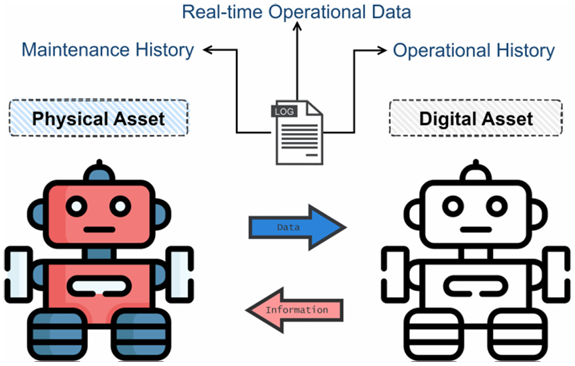
\includegraphics[width=0.85\textwidth]{images/DT_1.png}
	\caption{ساختار مفهومی دوقلوی دیجیتال شامل حلقه داده و اطلاعات بین فضای فیزیکی و فضای دیجیتال \cite{lopez2024madtwin}}
	\label{fig:dt-structure}
\end{figure}


\begin{figure}[H]
	\centering
	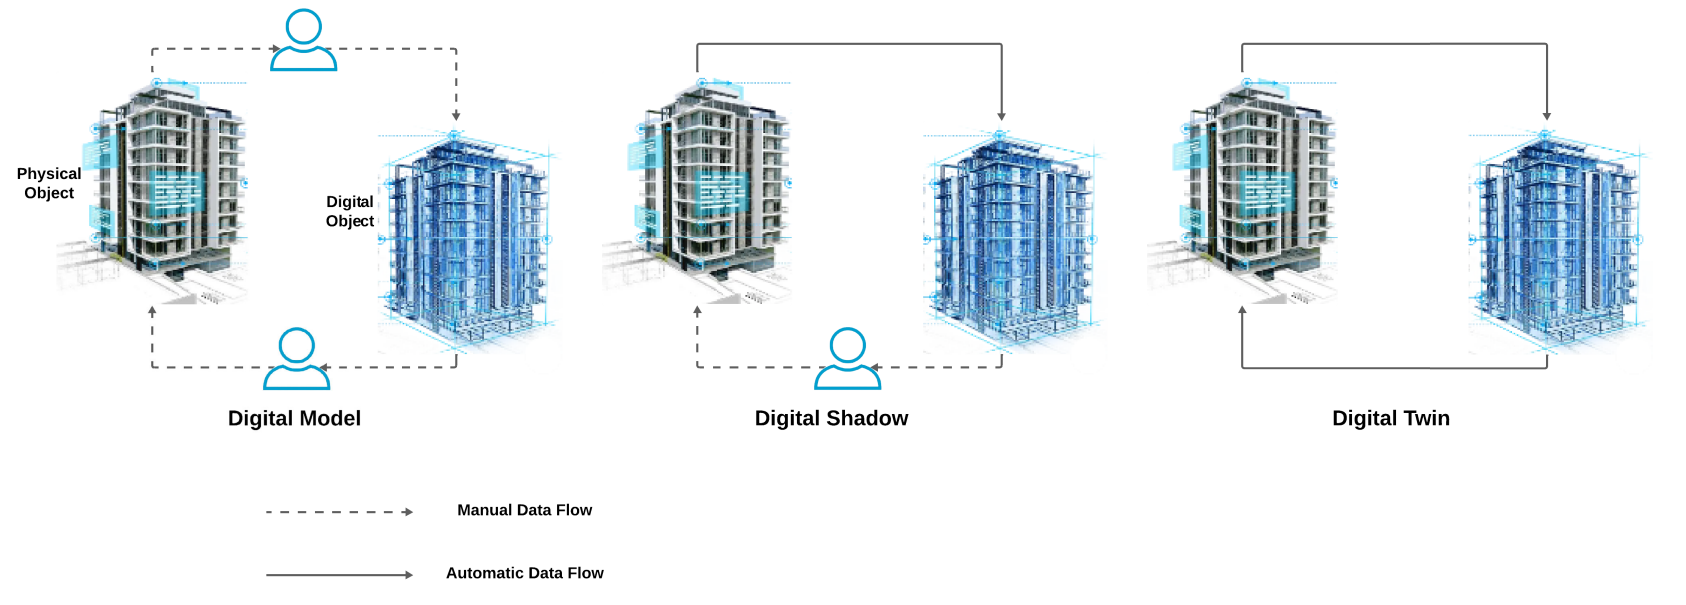
\includegraphics[width=0.85\textwidth]{images/DT_2.png}
	\caption{تفاوت بین \gls*{Digital Twins}، \gls*{DTSH} و \gls*{DTM} \cite{wang2024comprehensive}}
	\label{fig:dt-types}
\end{figure}


بر اساس مرور جامع پژوهش‌های اخیر، یکی از چالش‌های اساسی در توسعه و پیاده‌سازی دوقلوهای دیجیتال، دشواری در یکپارچه‌سازی کامل تمامی لایه‌ها در یک سامانه واحد است. این مسئله به دلیل پیچیدگی زیاد در اتصال اجزای فیزیکی، داده‌ای و مجازی، به‌ویژه در سیستم‌های چندعاملی، از اهمیت بالایی برخوردار است \cite{wang2024comprehensive,krizsinger2018digital,grieves2017digital}.

همان‌طور که در شکل \ref{fig:dt-types} نشان داده شده است، به‌منظور توصیف سطوح مختلف بلوغ و یکپارچگی دوقلوهای دیجیتال، می‌توان آن را بر اساس میزان اتصال میان جهان فیزیکی و دیجیتال، به سه سطح اصلی تقسیم‌بندی کرد \cite{krizsinger2018digital,fuller2020digital}:


\begin{enumerate}
\item 
\gls{DTM}:
در این سطح، ارتباط میان سامانه فیزیکی و نسخه دیجیتال آن به‌صورت دستی انجام می‌شود. داده‌ها از دنیای واقعی به مدل دیجیتال از طریق ورود اطلاعات انسانی منتقل می‌گردند و هیچ‌گونه همگام‌سازی خودکار میان این دو وجود ندارد. هرگونه تغییر در سامانه فیزیکی باید به‌صورت دستی در مدل دیجیتال اعمال شود. بنابراین، در این سطح هنوز مفهوم واقعی دوقلوی دیجیتال تحقق نیافته است و تنها یک مدل ایستا از سامانه ارائه می‌شود \cite{tao2019digital}.

\item 
\gls{DTSH}:
در این سطح، تعامل میان دنیای فیزیکی و مجازی به‌صورت \gls{Unidirectional} انجام می‌شود. به این معنا که تغییرات رخ‌داده در سامانه فیزیکی به‌طور خودکار در مدل دیجیتال بازتاب می‌یابد، اما برعکس آن ممکن نیست. در واقع، اطلاعات از دنیای واقعی به سمت فضای دیجیتال جریان دارد، اما هیچ تغییری از سوی مدل دیجیتال به دنیای فیزیکی منتقل نمی‌شود \cite{qi2021enabling,barricelli2019survey}.  
این رویکرد در بسیاری از کاربردهای پایش و تحلیل وضعیت تجهیزات رایج است، زیرا به‌سادگی امکان ثبت و نمایش رفتار واقعی را فراهم می‌سازد.

\item 
\gls{Digital Twins}:
در این لایه، ارتباط \gls{Bidirectional} میان دنیای فیزیکی و مدل دیجیتال برقرار است. تغییرات در هر یک از دو حوزه منجر به به‌روزرسانی خودکار دیگری می‌شود. این لایه موجب می‌شود تا مدل دیجیتال، بازنمایی دقیقی از وضعیت لحظه‌ای، تکامل و رفتار واقعی سامانه فیزیکی باشد \cite{tao2018digital,fuller2020digital,wang2024comprehensive}.  
دوقلوی دیجیتال نه‌تنها برای پیش‌بینی خرابی و نگهداری پیش‌بینانه، بلکه برای کنترل، تصمیم‌سازی خودکار، و تعامل بی‌درنگ میان انسان و سامانه نیز کاربرد دارد. در واقع، این سطح از بلوغ، نقطه نهایی در مسیر تحقق دوقلوی دیجیتال محسوب می‌شود که مبنای طراحی چارچوب چندلایه این پژوهش نیز قرار گرفته است.
\end{enumerate}

 
این طبقه‌بندی کمک می‌کند تا میزان پویایی و هوشمندی تعامل بین اجزای فیزیکی و مجازی را به‌صورت مرحله‌ای پیاده‌سازی و ارزیابی کرد. دوقلوی دیجیتال تنها یک مدل یا شبیه‌سازی ساده نیست، بلکه یک مدل زنده،‌ هوشمند و در حال تکامل و توسعه است که به عنوان یک همتای دیجیتال در دنیای مجازی، برای موجودیت حقیقی ایجاد می‌شود.




% ---------------------------------------
\subsection{عامل‌های هوشمند}

\gls{Intelligent Agent} موجودیتی نرم‌افزاری است که به‌صورت خودمختار عمل می‌کند، محیط را درک می‌کند و با تصمیم‌گیری مستقل اهداف خود را دنبال می‌کند \cite{wooldridge2009introduction}. 

ویژگی‌های عامل هوشمند عبارت‌اند از:
\begin{itemize}
	 \item \textbf{\gls{Autonomy}}: عملکرد بدون کنترل مستقیم انسان.
	\item \textbf{\gls{Reactivity}}: توانایی پاسخ سریع به تغییرات محیطی.
	\item \textbf{\gls{Proactiveness}}: اقدام آگاهانه برای دستیابی به اهداف.
	\item \textbf{\gls{Sociability}}: توانایی تعامل و ارتباط با عامل‌ها و انسان‌ها.
\end{itemize}

علاوه‌بر ویژگی‌هایی که بیان شد، عامل‌ها می‌توانند بسته به کارکرد خود، ویژگی‌های دیگری نیز داشته باشند. همچنین بنابر عملکرد آن‌ها، ممکن است برخی از این ویژگی‌ها را دارا نباشد. پس هر عامل را می‌توان بر اساس این ویژگی‌ها بررسی کرد.

بررسی پژوهش‌های اخیر نشان می‌دهد عامل‌هایی که با مدل‌های زبانی بزرگ، ترکیب شده‌اند، نسل جدیدی از عامل‌های هوشمند تعاملی را ایجاد کرده‌اند که می‌توانند از طریق زبان طبیعی دستورات را پردازش و اجرا کنند \cite{park2025interactive}.

%عکس
%\begin{figure}[H]
%	\centering
%	\includegraphics[width=0.75\textwidth]{figures/bdi-agent.png}
%	\caption{معماری عامل هوشمند مبتنی بر مدل BDI \cite{rao1995bdi}}
%	\label{fig:bdi-agent}
%\end{figure}

% ---------------------------------------
\subsection{سیستم‌های چندعاملی}

سیستم‌های چندعاملی \gls{MAS} مجموعه‌ای از عامل‌های مستقل هستند که به‌صورت توزیع‌شده با یکدیگر همکاری می‌کنند تا مسئله‌ای پیچیده را حل کنند \cite{dorri2018multiagent,bellifemine2007jade}. 

مزایای اصلی \gls{MAS} عبارت‌اند از:
\begin{enumerate}
	\item افزایش مقیاس‌پذیری در مسائل صنعتی.
	\item تصمیم‌گیری غیرمتمرکز و خودمختار.
	\item قابلیت تعامل و مذاکره بین عامل‌ها.
\end{enumerate}

%عکس
%\begin{figure}[H]
%	\centering
%	\includegraphics[width=0.8\textwidth]{figures/mas-structure.png}
%	\caption{نمای شماتیک ارتباط عامل‌ها در یک سیستم چندعاملی \cite{bellifemine2007jade}}
%	\label{fig:mas-structure}
%\end{figure}

در سیستم‌های چندعاملی می‌توان مسئله‌ها و وظیفه اصلی و بزرگ را به مسئله‌ها و وظیفه‌های کوچک‌تر تقسیم کرد و انجام هرکدام از آن‌ها را به عامل‌های جداگانه سپرد. با این کار می‌توان کارهای بزرگی که انجام آن‌ها توسط یک عامل بسیار سخت و پیچیده  و هزینه‌بر است را به راحتی انجام داد \cite{dorri2018multiagent}.


% ---------------

\subsection{هوش مصنوعی در دوقلوی دیجیتال}

امروزه کمتر حوزه‌ای می‌توان یافت که در آن هوش مصنوعی دخالت نداشته‌ باشد. در زمینه‌های مختلف، استفاده از روش‌ها و الگوریتم‌های هوش مصنوعی کاربرد فراوانی یافته است. 

هوش مصنوعی در اوایل ظهور خود، با
\gls{IoT}
پیوند خورد و محصولات تازه‌ای وارد بازار کرد. تعریف 
\gls{AIoT}
از ترکیب فناوری هوش مصنوعی و اینترنت اشیاء ایجاد شده‌است. در گذشته دوقلوی دیجیتال و هوش مصنوعی دو مفهوم کاملا مجزایی دانسته می‌شدند اما امروزه با گسترش و تنوع چشم‌گیر حسگر‌ها و همچنین پررنگ شدن اهمیت تحلیل داده‌ و پاسخگویی و اقدام هوشمندانه و سریع بر اساس داده، قابل جدا سازی نیستند. هوش مصنوعی به عنوان بخشی از لایه‌های دوقلوی دیجیتال کاملا پذیرفته شده و در حال استفاده است. این موضوع را می‌توان در کاربرد‌های متنوع دوقلو‌های دیجیتال مشاهده کرد.

دوقلوی دیجیتال به کمک هوش مصنوعی از داده‌های موجود در فرآیندها و موجودیت‌های واقعی، استفاده می‌کند تا بتواند تحلیل و پیش‌بینی‌های مورد نیاز را انجام دهد. این کارکرد نسبت به گذشته دوقلوی دیجیتال که تنها یک شبیه‌سازی و نمایش سه‌بعدی از فرآیند بود، بسیار کاربردی‌تر و مهم‌تر است \cite{rozbahani2023design}


% ---------------------------------------
\subsection{دوقلوهای دیجیتال چندعاملی}


\glspl{MA-DT}
ترکیبی از دو فناوری \glspl{MAS} و \glspl{Digital Twins} هستند که در آن هر دوقلو دیجیتال به عنوان یک عامل مستقل در محیط دیجیتال عمل می‌کند \cite{pretel2022masdt,wang2024multiagent}. این معماری به سیستم‌ها اجازه می‌دهد تا با تقسیم وظایف بین عامل‌های تخصصی، کارایی و سرعت تصمیم‌گیری را افزایش دهند. 

% عکس
%نوشتن بیشتر
%\begin{figure}[H]
%	\centering
%	\includegraphics[width=0.85\textwidth]{figures/madt-architecture.png}
%	\caption{نمونه‌ای از معماری دوقلوی دیجیتال چندعاملی در سامانه‌های صنعتی \cite{wang2024multiagent}}
%	\label{fig:madt-architecture}
%\end{figure}

در پژوهش‌های اخیر، از دوقلوهای چندعاملی برای پایش زنجیره تأمین، انرژی هوشمند و خطوط تولید استفاده شده است \cite{liu2024ai}. 


% ---------------------------------------
\subsection{مدل‌های زبانی بزرگ و دوقلوی دیجیتال}

مدل‌های زبانی بزرگ 
\glspl{LLM}
 مانند مدل‌های 
 \gls{GPT}\RTLfootnote{مانند 
 	\lr{GPT-4} و 
 	\lr{GPT-5}، سیستم‌های هوش مصنوعی قدرتمندی از 
 	\lr{OpenAI}
 	 هستند که برای درک و تولید متن شبیه به انسان طراحی شده‌اند و به عنوان ابزارهای همه‌کاره برای کدنویسی، نوشتن، خلاصه‌سازی و مکالمه عمل می‌کنند که همگی توسط یادگیری عمیق روی مجموعه داده‌های عظیم هدایت می‌شوند \cite{openai2025models}.}
 و 
 \lr{Grok}\RTLfootnote{
 یک چت‌بات هوش مصنوعی و مدل زبان بزرگ از
  \lr{xAI}
   است که به خاطر دسترسی بی‌درنگ به اطلاعات از \gls{Platform} 
  \lr{X}
    (توییتر) و استدلال پیشرفته شناخته می‌شود \cite{xai2025homepage}.
 }
  توانایی درک و تولید زبان طبیعی را دارند و می‌توانند در دوقلوهای دیجیتال برای تحلیل معنایی داده‌ها و تعامل بین انسان و ماشین به کار روند \cite{Pizon2026integrating,liu2025empoweringdt}. 



استفاده از ابزارهایی نظیر 
\lr{LangChain}
 و 
 \lr{Dify}
  به عامل‌های دوقلوی دیجیتال امکان می‌دهد تا با زبان طبیعی دستورات دریافت کنند، توضیحات فنی ارائه دهند و حتی استدلال خود را بیان کنند \cite{park2025interactive}.

% ---------------------------------------
%\subsection{جمع‌بندی}

%در این بخش از فصل، مفاهیم نظری مرتبط با دوقلوهای دیجیتال، سیستم‌های چندعاملی، یادگیری عمیق و مدل‌های زبانی بزرگ شرح داده شد. ترکیب این فناوری‌ها منجر به ایجاد نسل جدیدی از دوقلوهای دیجیتال چندعاملی می‌شود که قادر به تحلیل بی‌درنگ، تعامل زبانی و تصمیم‌گیری خودمختار در محیط‌های صنعتی هستند.
\section{مرور کارهای مرتبط}

\subsection{پژوهش‌های مرتبط با دوقلوهای دیجیتال}

در سال‌های اخیر، پژوهش‌های متعددی به بررسی مفاهیم، معماری‌ها و کاربردهای دوقلوهای دیجیتال  در صنایع مختلف پرداخته‌اند. در این بخش، پژوهش‌های مرتبط مرور شده‌اند تا چشم‌اندازی جامع از روند رشد و نوآوری‌های این حوزه ارائه شود.


در پژوهش 
وانگ، شو و ژانگ (۲۰۲۴)
  \cite{wang2024digitaltwin} یک مرور جامع از توسعه فناوری دوقلوی دیجیتال در صنایع مختلف ارائه شده است. این پژوهش بر مدل‌سازی داده‌محور و استفاده از الگوریتم‌های یادگیری ماشین برای همگام‌سازی داده‌های فیزیکی و مجازی تمرکز دارد و به چالش‌های همگرایی داده در سیستم‌های ناهمگون اشاره می‌کند. نویسندگان یک چارچوب چهاربخشی برای پیاده‌سازی کارایی دوقلوهای دیجیتال معرفی کرده‌اند که هدف آن کاهش تأخیر و افزایش دقت همگام‌سازی داده‌ها بین دنیای واقعی و مدل مجازی است. نوآوری اصلی این پژوهش، ارائه‌ی مدل ترکیبی داده‌محور برای بهبود کارایی در انتقال و تحلیل داده‌های صنعتی است.

در پژوهش
ژو، لی و چن (۲۰۲۵)
 \cite{zhou2025newera} روند تحول دوقلوهای دیجیتال در \gls{Industry45} تحلیل شده است. این مطالعه، که بر داده‌های به‌دست‌آمده از ۴۳ شرکت بین‌المللی تکیه دارد، نشان می‌دهد استفاده از دوقلوهای دیجیتال در زمینه‌های نگهداری پیش‌بینانه، طراحی سیستم و مدیریت انرژی به‌صورت چشمگیری افزایش یافته است. نویسندگان، شاخصی با عنوان «\gls{IDTAI}» را معرفی کرده‌اند که میزان آمادگی سازمان‌ها در پذیرش فناوری دوقلوی دیجیتال را اندازه‌گیری می‌کند. این شاخص برای نخستین بار به‌صورت کمی میزان نفوذ فناوری دوقلوی دیجیتال در صنایع را می‌سنجد.

 

گزارش صنعتی منتشرشده توسط شرکت
ایرباس (۲۰۲۵)
\cite{airbus2025digitaltwins} به تشریح پیاده‌سازی گسترده دوقلوهای دیجیتال در سامانه 
 \lr{ } \cite{airbus2024skywisecorex}
  پرداخته است. در این سیستم بیش از ۱۲٬۰۰۰ هواپیما از مدل‌های دوقلوی دیجیتال برای نظارت و نگهداری پیش‌بینانه استفاده می‌کنند. این گزارش نشان می‌دهد که استفاده از دوقلوی دیجیتال باعث کاهش زمان خرابی‌های برنامه‌ریزی‌نشده، بهبود بهره‌وری عملیاتی و افزایش ایمنی پروازها شده است. نوآوری کلیدی این پروژه، پیاده‌سازی دوقلو دیجیتال در مقیاس واقعی و استفاده از یادگیری ماشین برای تحلیل جریان داده‌های پروازی است.


در پژوهش
آریدی، آریدی، بیگود و لمنان (۲۰۲۶)
\cite{aridi2026theoretical}
مبانی نظری و ارزش‌های عملی فناوری دوقلوهای دیجیتال در قالب یک مرور جامع بررسی شده است. نویسندگان با تحلیل ۱۴۶ مطالعهٔ علمی منتشرشده در پایگاه‌های معتبر، روند تحول دوقلوهای دیجیتال را از کاربردهای اولیه در تولید تا استفاده از آن‌ها در حوزه‌های چندرشته‌ای بررسی کرده‌اند. نتایج این مطالعه نشان می‌دهد که اگرچه بخش قابل‌توجهی از پژوهش‌ها بر ایجاد مدل‌های مجازی و همگام‌سازی آن‌ها با موجودیت فیزیکی تمرکز دارند، فاصلهٔ محسوسی میان توسعهٔ نظری و تحقق ارزش عملی دوقلوهای دیجیتال در محیط‌های واقعی وجود دارد. این پژوهش همچنین بر اهمیت فناوری‌های مکمل، از جمله زنجیرهٔ بلوکی، برای افزایش یکپارچگی داده، امنیت و قابلیت اعتماد در ارتباط میان بخش فیزیکی و مجازی تأکید می‌کند. نوآوری اصلی این مطالعه، ارائهٔ تصویری یکپارچه از مبانی نظری، کاربردهای عملی و موانع موجود برای ایجاد ارزش توسط دوقلوهای دیجیتال است.



در پژوهش
بوانش و همکاران (۲۰۲۶)
\cite{bhuvanesh2026selflearningdt}
چارچوبی با عنوان
\lr{Self-Learning Digital Twin}
برای بهینه‌سازی پیوستهٔ بهره‌وری انرژی در تجهیزات اینترنت اشیا ارائه شده است. در این چارچوب، دوقلوی دیجیتال با استفاده از سازوکارهای یادگیری مستمر، رفتار تجهیزات را از روی داده‌های عملیاتی تحلیل کرده و تنظیمات مناسب را برای کاهش مصرف انرژی پیشنهاد می‌دهد. برخلاف معماری‌های ایستا که تنها وضعیت جاری تجهیز را بازنمایی می‌کنند، چارچوب پیشنهادی قابلیت سازگاری تدریجی با شرایط جدید و بهبود تصمیم‌های کنترلی را دارد. نوآوری اصلی این پژوهش، ترکیب دوقلوی دیجیتال با یادگیری خودکار و بهینه‌سازی مستمر در محیط‌های محدود از نظر منابع است. این یافته نشان می‌دهد که دوقلوهای دیجیتال می‌توانند از یک مدل صرفاً توصیفی به یک مؤلفهٔ تصمیم‌گیر و سازگارشونده در سامانه‌های هوشمند تبدیل شوند.



\subsection{پژوهش‌های مرتبط با دوقلوهای دیجیتال چندعاملی}

در پژوهش \cite{lopez2024madtwin}، 
لوپز و همکاران (۲۰۲۴)
چارچوبی با عنوان \lr{MADTwin} برای توسعه دوقلوهای دیجیتال چندعاملی در محیط‌های انبارداری هوشمند ارائه کرده‌اند. در این چارچوب، هر عامل نمایانگر یک جزء فیزیکی (مانند ربات یا سامانه جابجایی کالا) است و با دوقلوی دیجیتال متناظر خود در محیط مجازی همگام می‌شود. این پژوهش بر مبنای فناوری‌های 
 \gls{IoT}
  و سامانه‌های چندعاملی طراحی شده و امکان تعامل بی‌درنگ میان موجودیت‌های فیزیکی و دیجیتال را فراهم می‌کند. \textbf{نوآوری} ارائه‌ی چارچوبی مبتنی بر عامل با قابلیت خودسازماندهی برای بهینه‌سازی فرآیندهای حمل‌ونقل و تصمیم‌گیری توزیع‌شده در محیط‌های صنعتی پیچیده است.

در پژوهش \cite{almeida2025healthagentsdt}، 
آلمیدا و همکاران (۲۰۲۵)
 به بررسی امکان ادغام سامانه‌های چندعاملی با دوقلوهای دیجیتال در حوزه مراقبت سلامت پرداخته‌اند. این پژوهش یک معماری ترکیبی برای نظارت بر بیماران و شبیه‌سازی رفتارهای بالینی ارائه می‌کند که در آن عامل‌ها نقش هماهنگ‌کننده تعامل بین داده‌های فیزیکی بیماران و مدل دیجیتال را بر عهده دارند. 


در پژوهش
گائو و همکاران (۲۰۲۶)
\cite{gao2026selfevolving}
چارچوبی برای ایجاد دوقلوهای دیجیتال خودتکامل‌یابنده در خطوط تولید انعطاف‌پذیر ارائه شده است. این چارچوب با استفاده از یک سامانهٔ چندعاملی مبتنی بر مدل زبان بزرگ، دوقلوی دیجیتال را در سه بُعد دانش، رفتار و هندسه تجزیه می‌کند و از یک گراف دانش تکامل‌یابنده برای به‌روزرسانی مدل مجازی بهره می‌گیرد. در معماری پیشنهادی، عامل‌ها وظایفی مانند تفسیر وضعیت خط تولید، هماهنگی عملیات، شناسایی خطا و پشتیبانی از تصمیم‌گیری را به‌صورت توزیع‌شده انجام می‌دهند. ارزیابی چارچوب در یک خط تولید شامل پایش عیب و دسته‌بندی قطعات نشان داده است که استفاده از این معماری می‌تواند زمان تغییر محصول و بازیابی خطا را کاهش دهد و نرخ هشدارهای نادرست را بهبود بخشد. نوآوری اصلی این پژوهش، ارائهٔ چارچوبی برای پیوند مدل‌های زبانی بزرگ با سامانه‌های چندعاملی و دوقلوهای دیجیتال خودتکامل‌یابنده است. چارچوبی که دوقلوی دیجیتال را از یک بازنمایی منفعل به یک سامانهٔ هماهنگ‌کننده و تصمیم‌گیر تبدیل می‌کند.



در مطالعه
کولیبالی و هملیش (۲۰۲۶)
\cite{coulibaly2026madtdt}
معماری‌ها، فناوری‌ها و چالش‌های باز مربوط به دوقلوهای دیجیتال مبتنی بر سامانه‌های چندعاملی برای نگهداشت پیش‌بینانه بررسی شده است. نویسندگان با انجام یک مرور نظام‌مند، یک رده‌بندی ساختاریافته از معماری‌های ترکیبی
\lr{MAS--DT}
ارائه کرده و معماری سه‌لایه‌ای شامل لبه، مه و ابر را به‌عنوان یکی از مسیرهای مناسب برای استقرار توزیع‌شدهٔ این سامانه‌ها پیشنهاد داده‌اند. نتایج مطالعه نشان می‌دهد که سامانه‌های چندعاملی می‌توانند برای هماهنگی بین چند تجهیز، توزیع پردازش، تصمیم‌گیری محلی و مدیریت وضعیت دوقلوهای دیجیتال به کار گرفته شوند. بااین‌حال، محدودیت منابع سخت‌افزاری، نیاز به \glspl{Protocol}ی ارتباطی سبک، هماهنگی بین چند گره و تفسیرپذیری تصمیم‌ها همچنان از چالش‌های مهم این حوزه هستند. نویسندگان همچنین تخمین عمر باقیمانده، هوش مصنوعی قابل‌تفسیر و \gls{Orchestration} سلسله‌مراتبی دوقلوها را از مهم‌ترین مسیرهای پژوهشی آینده معرفی کرده‌اند. نوآوری این پژوهش در ارائهٔ یک چارچوب مفهومی منسجم برای ترکیب سامانه‌های چندعاملی و دوقلوهای دیجیتال در نگهداشت پیش‌بینانه و مشخص کردن فاصلهٔ موجود میان معماری‌های پژوهشی و سامانه‌های صنعتی قابل‌استقرار است.









\subsection{پژوهش‌های مرتبط با کاربرد مدل‌های زبانی بزرگ در دوقلوهای دیجیتال}

پیژون، وویچیک و گولا (۲۰۲۶) در پژوهش 
\cite{Pizon2026integrating} چارچوبی مفهومی برای سامانه پشتیبان مدیریت تولید ارائه کرده‌اند که در آن مدل‌های زبانی بزرگ با دوقلوهای دیجیتال یکپارچه می‌شوند تا تعامل طبیعی کاربر با سامانه ممکن شود. این چارچوب با ایجاد یک دوقلوی دیجیتال هوشمند در نقش کارشناس تولید، به چالش پراکندگی داده‌ها پاسخ می‌دهد و امکان استدلال زمینه‌ای، تلفیق اطلاعات از منابع گوناگون و پشتیبانی بلادرنگ از تصمیم‌گیری را فراهم می‌آورد. نویسندگان نشان می‌دهند که بهره‌گیری از قابلیت‌های مدل‌های زبانی در تشخیص الگو، تحلیل پیش‌بینانه و تولید توصیه‌های خودکار می‌تواند مدیریت تولید را از حالت واکنشی به رویکردی فعال و پیش‌نگر سوق دهد.



در پژوهش \cite{patel2024llmdt}،
پاتل، سینگ و کومار (۲۰۲۴)
   به استفاده از \lr{ChatGPT} در تحلیل بی‌درنگ داده‌های تولید پرداخته‌اند. نویسندگان نشان داده‌اند که مدل‌های زبانی می‌توانند وضعیت غیرعادی سیستم‌ها را تشخیص داده و هشدارهای متنی تولید کنند. نوآوری در «تعامل زبانی انسان–دوقلو دیجیتال» است که تجربه کاربری را به‌طور چشمگیری بهبود می‌بخشد.



\subsection{پژوهش‌های مرتبط با مجموعه داده \lr{CMAPSS}}

در پژوهش
 \cite{smith2025cmapsslinear}،
اسمیت، رائو و پاتل (۲۰۲۵)
    مدل‌های خطی برای پیش‌بینی عمر باقیمانده 
    \glspl{Turbofan}
     را با استفاده از داده‌های 
	 \lr{C-MAPSS} ناسا بررسی کرده‌اند. نویسندگان نشان داده‌اند که مدل‌های خطی ساده در صورت \gls{Normalization} مناسب، می‌توانند کارکرد قابل‌مقایسه‌ای با شبکه‌های عمیق داشته باشند. نوآوری آن‌ها در تحلیل اثر \gls{Noise} سنجش و بهینه‌سازی وزن ویژگی‌ها است.

	

در پژوهش
تانگ (۲۰۲۶)
\cite{tang2026sensorfailure}
یک چارچوب یادگیری عمیق برای پیش‌بینی عمر باقیمانده موتورهای توربوفن در شرایط خرابی بخشی حسگرها ارائه شده است. نویسنده برای بازسازی پارامترهای ازدست‌رفته از یک مولد مبتنی بر شبکه مولد تخاصمی با گرادیان جریمه‌شده استفاده کرده و سپس خروجی بازسازی‌شده را به یک پیش‌بین ترکیبی
\lr{CNN--LSTM}
برای تخمین عمر باقیمانده وارد کرده است. روش پیشنهادی با استفاده از مجموعه‌دادهٔ \lr{CMAPSS} ارزیابی شده و هدف اصلی آن حفظ دقت پیش‌بینی در شرایطی است که بخشی از حسگرها دچار خرابی یا قطع داده شده‌اند. نتایج نشان می‌دهد که ترکیب بازسازی داده و مدل‌سازی هم‌زمان ویژگی‌های مکانی و زمانی می‌تواند نسبت به روش‌های پایه، پایداری بیشتری در برابر داده‌های ناقص ایجاد کند. نوآوری اصلی این پژوهش، طراحی یک چارچوب مقاوم برای پیش‌بینی \gls{RUL} در شرایط خرابی حسگر و نزدیک کردن مسئلهٔ پیش‌بینی به شرایط واقعی سامانه‌های صنعتی است.




با وجود پیشرفت‌های یادشده، بیشتر این پژوهش‌ها فاقد چارچوبی جامع هستند که بتوانند تحلیل سری‌های زمانی را در سطح سیستم‌های چندعاملی و با تعامل هوشمند مدل‌های زبانی بزرگ، ترکیب کنند.




\subsection{تحلیل شکاف‌های پژوهشی و جمع‌بندی}
بر اساس بررسی‌های انجام‌شده، چندین شکاف کلیدی در پژوهش‌های پیشین شناسایی می‌شود:
\begin{itemize}
	\item
	 بیشتر پژوهش‌های 
	\glspl{MAS} و
	\glspl{Digital Twins}
	 فاقد قابلیت تفسیرپذیری تصمیمات و تعامل زبانی طبیعی با کاربران هستند.
	 
	\item
	 مطالعات مبتنی بر 
	ترکیب مدل‌های زبانی بزرگ و دوقلوهای دیجیتال
	 هنوز در مراحل اولیه‌اند و بیشتر بر تحلیل داده‌های متنی تمرکز دارند تا بر سیستم‌های صنعتی پویا.
	 
	\item
	 در حوزه پیش‌بینی عمر باقیمانده در مجموعه داده \lr{CMAPSS}، مسئله 
	 \gls{Underestimate}،
	  همچنان چالشی مهم است که منجر به تصمیم‌های نادرست در نگهداری پیش‌بینانه می‌شود و اعتماد را به پیش‌بینی‌های انجام‌شده توسط هوش مصنوعی، غیرقابل اعتماد می‌کند.
	
	\item
	در حوزه پیش‌بینی عمر باقی‌ مانده برای \gls{Turbofan} در مجموعه‌داده 
	\lr{CMAPSS}
		ناسا، بیشتر پژوهش‌ها صرفاً بر بهبود دقت مدل‌های پیش‌بینی (مانند شبکه‌های \lr{LSTM}) متمرکز بوده‌اند و به توضیح‌پذیری نتایج و تحلیل سهم هر حسگر در تصمیم نهایی مدل توجهی نکرده‌اند.
	
	
\end{itemize}

بنابراین، این پایان‌نامه با هدف پوشش این شکاف، چارچوبی پنج‌لایه برای ادغام سیستم‌های چندعاملی، دوقلوهای دیجیتال و مدل‌های زبانی بزرگ در تحلیل و پیش‌بینی مجموعه داده \lr{CMAPSS} ارائه می‌دهد تا ضمن افزایش دقت پیش‌بینی، امکان تعامل هوشمند و تصمیم‌گیری توضیح‌پذیر را فراهم آورد.


%برای بیان اکرونیم یک کلمه مانند  \gls{LASSO}، به این صورت عمل کنید.
%   \gls{ML}
%   یا 
%   \gls{DL}
%   یا
%   \gls{FN}
%   یا 
%   \gls{TN}
%   یا
%   \gls{LSTM}
%   یا 
%   \gls{SGL}
%   یا
%   \gls{TP}
%   یا 
%   \gls{FP}

%\subsection{زیربخش \gls*{1st}}\label{sec:brain:sub_brain}
%این یک متن نمونه است که به سه مرحله \gls{1st}،
% \gls{2nd} و \gls{3rd} تقسیم می‌شود. 
% 
% برای معادل جمع فارسی در دیکشنری اینطور فراخوان کنید: \glspl{2nd}
%\begin{itemize}
%	\item
%	\gls{1st}: 
%	این یک آیتم نمونه است...
%		\item 
%	\gls{2nd}: 
%	این یک آیتم نمونه است...
%	\item 
%	\gls{3rd}: 
%	این یک آیتم نمونه است...
%\end{itemize}
%
%\subsection{زیربخش دوم}\label{sec:brain:second_sub}
%این یک متن نمونه است...
%
%
%\paragraph{پاراگراف نمونه \gls*{1st}}
%این یک متن نمونه است...
%\paragraph{پاراگراف نمونه \gls*{2nd}}
%این یک متن نمونه است...
%
%\section{معرفی \gls*{dataset}}\label{sec:dataset}
%این بخش نمونه است...
%
%\begin{enumerate}
%	
%\item\textbf{فاز اول یا \lr{English-1}:} 
%این یک متن نمونه است.
%\begin{itemize}
%	\item 
%	این یک آیتم نمونه است...
%	\item 
%	این یک آیتم نمونه است...
%	\item 
%	این یک آیتم نمونه است...
%\end{itemize}
%
%این یک متن نمونه است...
%
%\item\textbf{فاز دوم یا \lr{English-2}:} 
%این یک متن نمونه است...
%
%\item\textbf{فاز سوم یا \lr{English-3}:} 
%این یک متن نمونه است...
%\end{enumerate}
%
%برای کامنت کردن بخشی از پروژه بدون حذف آن، از این دستور استفاده کنید.
%\begin{comment}
%برای کامنت کردن بخشی از پروژه بدون حذف آن، از این دستور استفاده کنید.
%\end{comment}
%
%برای درج جدول \ref{tab:my_table1} و رفرنس‌دهی از این کد استفاده کنید.
%
%\begin{table}[t!]
%	\centering
%	\caption{جدول نمونه افقی}
%	\label{tab:my_table1}
%%	\begin{tabular}{rccccc}
%%		\toprule			
%%		$\text{گروه}$ && $\text{فارسی (English)}$ & $\text{فارسی English}$ & $\text{فارسی English}$ & $\text{فارسی English}$ \\
%%		\midrule
%%		\rl{جنسیت}&(\rl{مرد - زن})	
%%		& $10 - 20$ & $10 - 20$ & $10 - 20$ & $10 - 20$
%%		\\
%%		\bottomrule
%%	\end{tabular}
%\end{table}
%
%برای درج جدول عمودی \ref{tab:my_table2} و رفرنس‌دهی از این کد استفاده کنید.
%\begin{sidewaystable}
%	\begin{threeparttable}
%		\caption{جدول نمونه عمودی}
%		\label{tab:my_table2}
%		\setlength\tabcolsep{0pt} % make LaTeX figure out intercolumn spacing
%		
%%		\begin{tabular*}{\columnwidth}{@{\extracolsep{\fill}} cccccccccc}
%%			\toprule			
%%			$\text{گروه}$ & 
%%			$\myfrac{\text{جنسیت}}{\text{مرد - زن}}$ & 
%%			$\myfrac{\text{فارسی}}{\text{\lr{mean$\pm $std}}}$ & 
%%			$\myfrac{\text{ٍenglish}}{\text{\lr{mean$\pm $std}}}$ & 
%%			$\myfrac{\text{فارسی}}{\text{\lr{mean$\pm $std}}}$ & 
%%			$\myfrac{\text{\lr{english}}}{\text{\lr{mean$\pm $std}}}$ & 
%%			$\myfrac{\text{\lr{ٍenglish}}}{\text{\lr{mean$\pm $std}}}$ & 
%%			$\myfrac{\text{ٍenglish}}{\text{\lr{mean$\pm $std}}}$ & 
%%			$\myfrac{\text{\lr{ٍenglish}}}{\text{\lr{mean$\pm $std}}}$ & 
%%			$\myfrac{\text{\lr{RAVALT-PF}}}{\text{\lr{mean$\pm $std}}}$ \\
%%			\midrule
%%			فارسی AD & $189 / 153$ & $75.0 \pm 7.8$ & $4.39 \pm 1.67$ & $15.2 \pm 3.0$ & $19.6 \pm 6.7$ & $29.9 \pm 8.1$ & $23.2 \pm 2$ & $22.8 \pm 7.6$ & $89.0 \pm 21.2$ 
%%			\\
%%			\bottomrule
%%		\end{tabular*}
%	\end{threeparttable}
%\end{sidewaystable}
%
%\section{فرمول}\label{sec:formula}
%بنابراین برای هر نقطه $X$ از تصویر سه بعدی دریافتی، رابطه
%\begin{align} \label{eq:n3-main}
%	v(X) = u(X) f(X) + n(X)
%\end{align}
%برقرار است که $v$ سیگنال اندازه‌گیری شده، $u$ سیگنال مورد انتظار بدون اثر \gls{bias} میدان و $f$ یک سیگنال با تغییرات آرام و نماینده \gls{bias} میدان است.
%روابط تبدیل فوریه تابع $f(t)$ و معکوس آن به بیان شده در روابط \ref{eq:fourier} و \ref{eq:afourier}  هستند.
%\begin{align}\label{eq:fourier}
%\mathcal{F}(f(t))= F(w)=\sum_{k=0}^{N-1}f_k e^{-i\frac{2\pi}{N}kn}
%\end{align}
%\begin{align}\label{eq:afourier}
%f_k= F(w)=\frac{1}{N}\sum_{n=0}^{N-1}\mathcal{F}_n e^{-i\frac{2\pi}{N}kn}
%\end{align}


%*****************************************************************
% chap3.tex
%*****************************************************************

% فصل ۳
\chapter{روش‌شناسی و معماری پیشنهادی}\label{chap:methodology}


% -----------------------------------------------------------------------
\section{رویکرد کلی پژوهش}\label{sec:method-approach}

بررسی پژوهش‌های پیشین در فصل دوم نشان داد که حوزه پیش‌بینی \gls{RUL} و پایش تجهیزات صنعتی با چند شکاف بنیادین روبه‌روست. نبود چارچوبی یکپارچه که \glspl{MAS}، \glspl{Digital Twins} و \glspl{LLM} را در یک معماری منسجم ترکیب کند؛ غفلت از توضیح‌پذیری نتایج پیش‌بینی و نقش حسگرهای مختلف در تصمیم مدل و بی‌توجهی به هزینه نامتقارن خطای بیش‌برآورد در \gls{predictive maintenance}. این فصل پاسخ روش‌شناختی پژوهش حاضر به این شکاف‌ها را ارائه می‌دهد.

روش‌شناسی پژوهش حاضر به صورت خطی و یک مرحله‌ای نیست. پس از بررسی پژوهش‌های مرتبط در حوزه دوقلوی دیجیتال، \glspl{MAS} و کاربردهای صنعتی، کار در دو شاخه ادامه می‌یابد. شاخه نخست به انتخاب مجموعه داده \gls{CMAPSS} و سپس مرور پژوهش‌های تازه‌تر --- از جمله پیش‌بینی \gls{RUL} با \gls{LSTM} و ادغام \gls{LLM} با دوقلوهای دیجیتال --- می‌پردازد. شاخه دوم معماری پنج‌لایه چندعاملی را طراحی می‌کند. این دو شاخه در شناسایی شکاف‌ها به هم می‌رسند تا معماری پیشنهادی به مسائل موجود در شکاف‌های شناسایی شده پاسخ دهد. نبود سامانه و معماری یکپارچه دوقلوی دیجیتال، ضعف توضیح‌پذیری توسط حسگر‌ها و هزینه نامتقارن خطا در پیش‌بینی مجموعه‌داده \gls{CMAPSS} از جمله آن مسائل است. پس از آن، نمونه‌سازی آزمایشگاهی و ارزیابی تجربی انجام می‌شود. شکل \ref{fig:method-flow} این مسیر هفت مرحله‌ای را نشان می‌دهد.


در سمت چپ شکل \ref{fig:method-flow}، انتخاب \gls{CMAPSS} مرور ادبیات را به کارهای مسئله‌محور محدود می‌کند که شامل پژوهش‌های متنوع در زمینه این مجموعه داده است. در سمت راست، ادبیات پایه‌ای به طراحی مفهومی لایه‌ها، عامل‌ها و \gls{Protocol} تعامل می‌پردازد. نقطه تلاقی این دو شاخه مرحله شکاف‌هاست. معماری باید یکپارچگی چندعاملی، توضیح سهم حسگرها و سوگیری آگاهانه به کم‌برآورد را پوشش دهد. مرحله ششم این طراحی را روی داده شبیه‌سازی‌شده پیاده می‌کند و سطح بلوغ هدف را از \gls{DTSH} یک‌طرفه به \gls{Digital Twins} با ارتباط \gls{Bidirectional} در بستر شبیه‌سازی می‌رساند \cite{tao2019digital}. مرحله پایانی معیارهای کمی پیش‌بینی، نسبت خطای کم‌برآورد و کیفیت توضیح عامل زبانی را ارائه می‌دهد.


در خصوص هزینه نامتقارن خطا، پژوهش حاضر رویکردی متمایز دارد. در \gls{predictive maintenance}، بیش‌برآورد \gls{RUL} --- یعنی پیش‌بینی بیشتر از عمر واقعی تجهیز --- می‌تواند باعث خرابی ناگهانی و ایجاد هزینه قابل توجه شود. در مقابل، کم‌برآورد عمر، اگرچه ممکن است بررسی تجهیز را زود‌تر از زمان واقعی، پیشنهاد دهد اما خطر خرابی را به‌شدت کاهش می‌دهد. بنابراین پژوهش حاضر تابع هزینه‌ای طراحی می‌کند که خطاها را آگاهانه به سمت کم‌برآورد سوق می‌دهد. به این معنا که اگر مدل در پیش‌بینی اشتباه کند، عمر باقیمانده را کمتر از واقعیت برآورد می‌کند، نه بیشتر. این انتخاب آگاهانه، یک انتخاب محافظه‌کارانه و ایمن در فرآیندهای صنعتی واقعی است.


\begin{figure}[H]
	\centering
	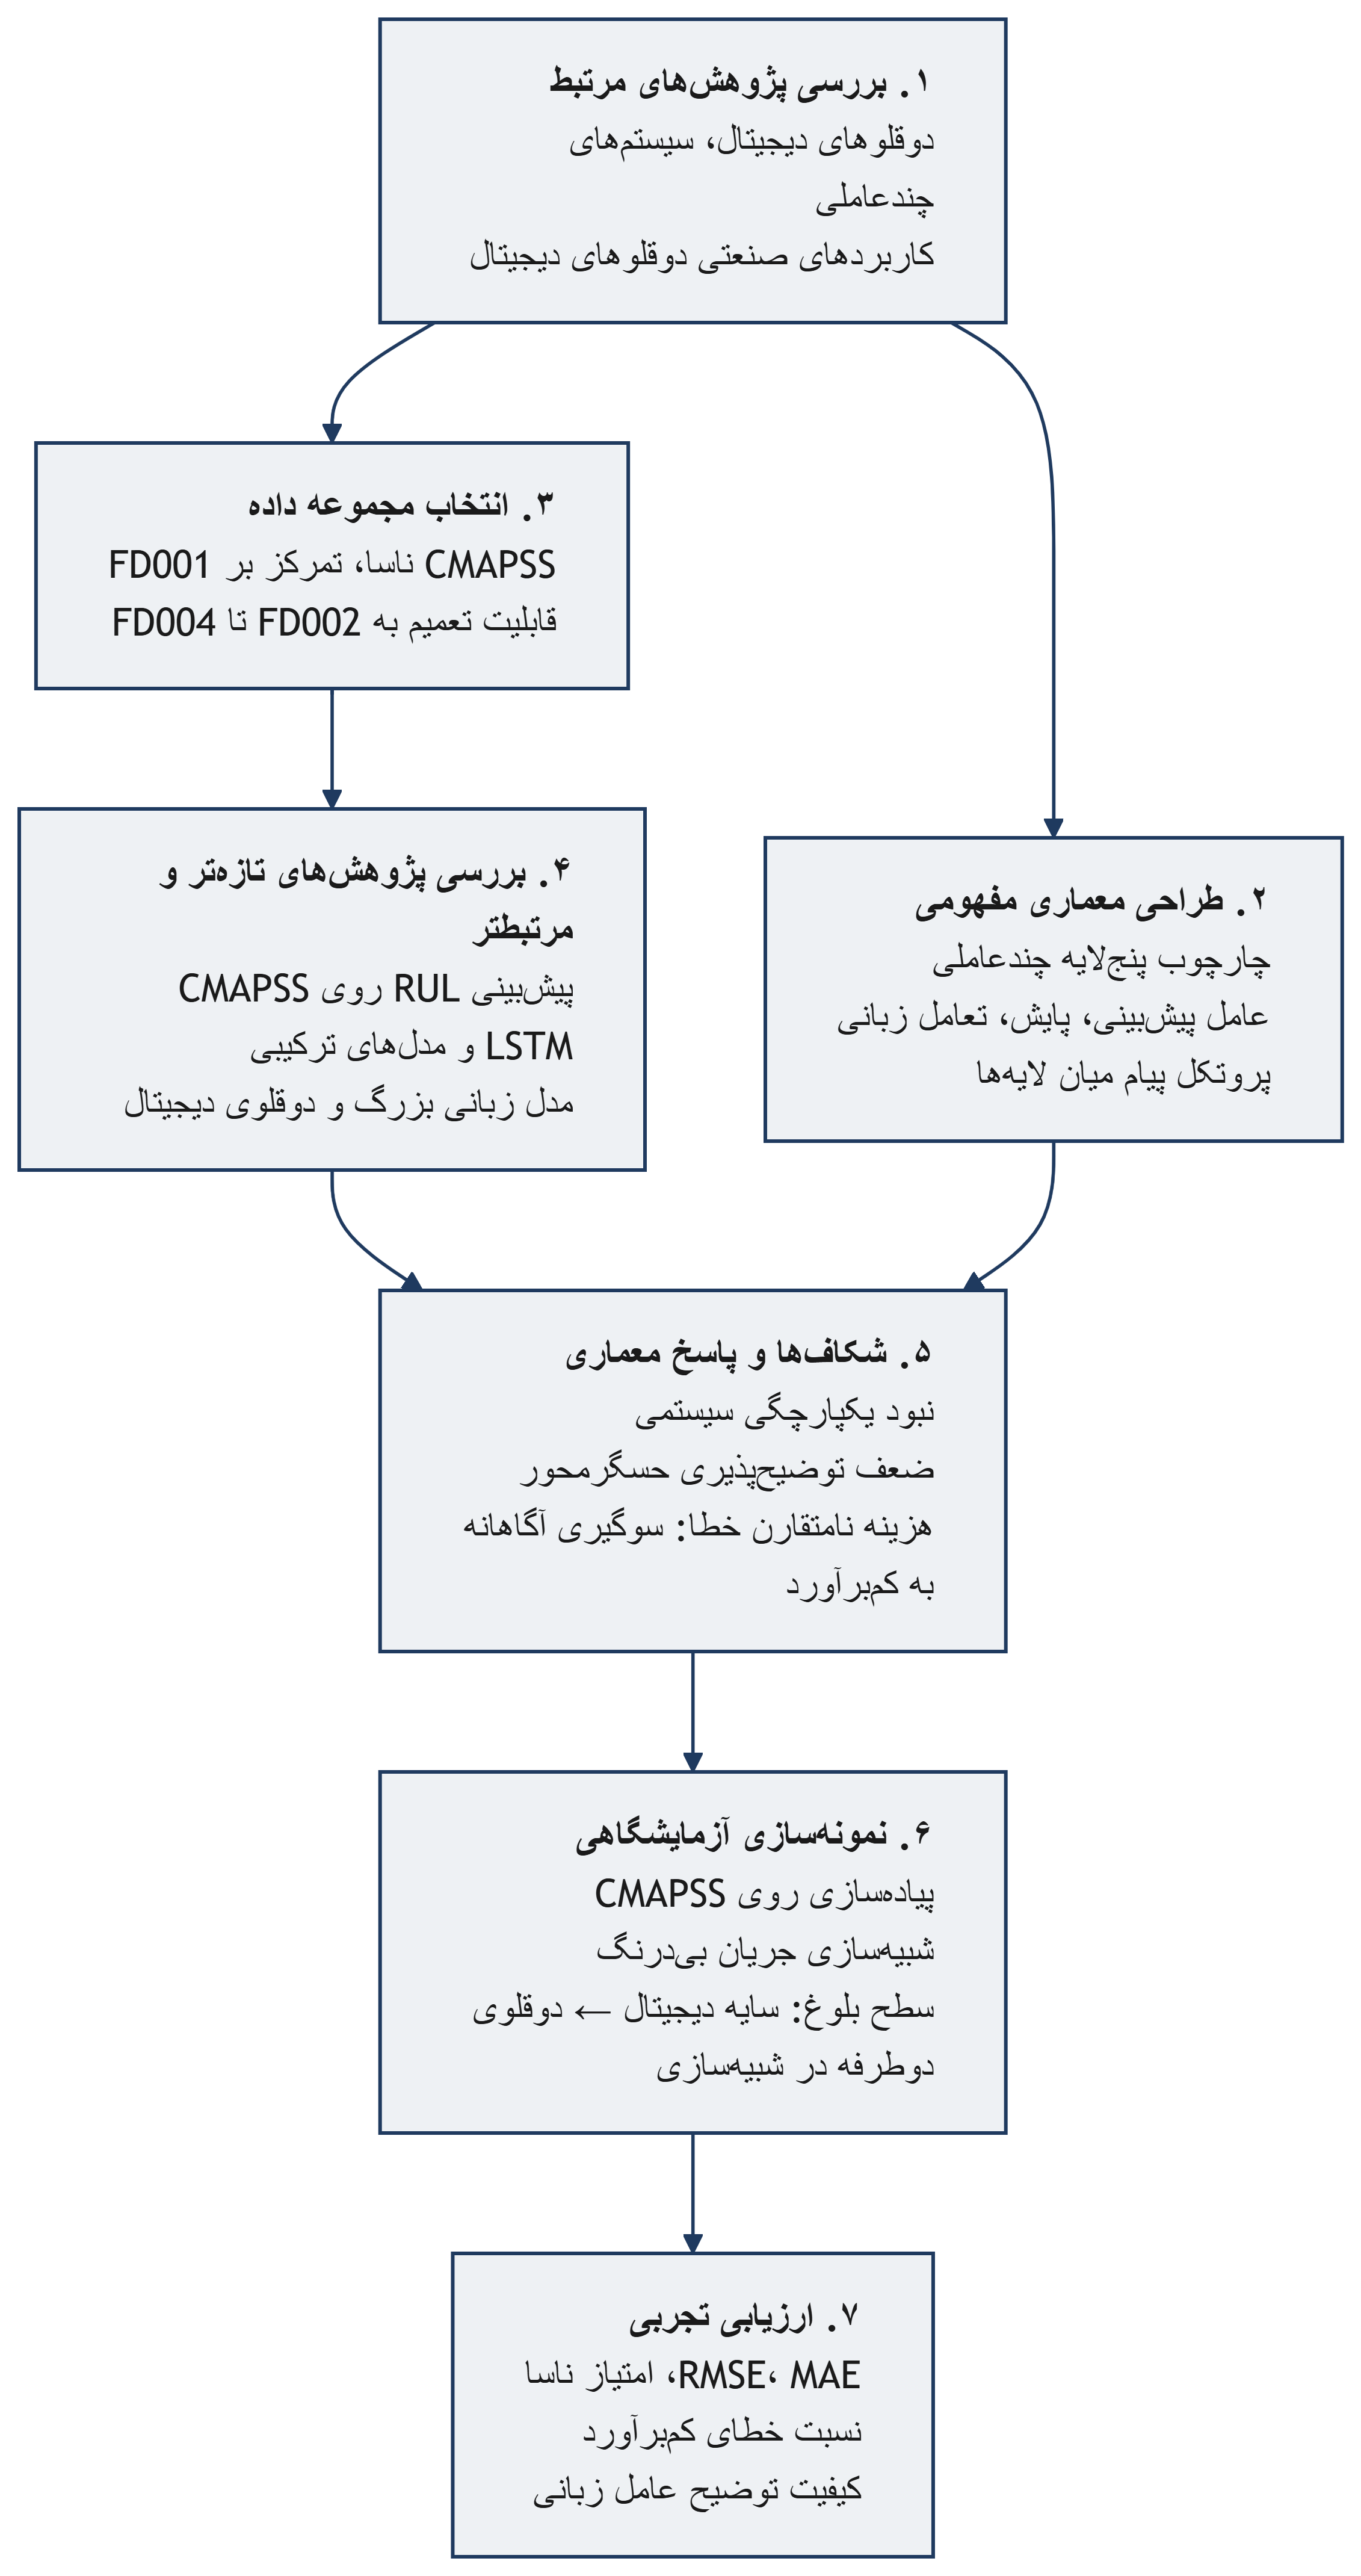
\includegraphics[width=0.8\textwidth]{images/method_flow.png}
	\caption{
		مسیر هفت‌ مرحله‌ای پژوهش که پس از بررسی پژوهش‌های مرتبط، دو شاخه موازی  می‌شود و انتخاب داده به همراه طراحی معماری پیش می‌رود. در شناسایی شکاف‌ها به هم می‌رسند و در نهایت ارزیابی صورت می‌گیرد.}
	\label{fig:method-flow}
\end{figure}


% -----------------------------------------------------------------------


% -----------------------------------------------------------------------
\section{معماری پیشنهادی دوقلوی دیجیتال چندعاملی}
\label{sec:architecture}

\subsection{نمای کلی و اصول طراحی}
\label{sec:arch-overview}

معماری پیشنهادی این پژوهش، یک چارچوب پنج‌لایه برای پیاده‌سازی \gls{MA-DT} در سامانه‌های پایش و نگهداری پیش‌بینانه است که با هدف ایجاد یک زنجیره یکپارچه از موجودیت فیزیکی تا تصمیم‌گیری سطح‌بالا طراحی شده است. ایده اصلی معماری آن است که داده‌های تولیدشده توسط موجودیت فیزیکی، پس از جمع‌آوری و آماده‌سازی، در یک لایه دیجیتال متشکل از عامل‌های دوقلوی دیجیتال بازنمایی شوند و سپس عامل‌های کاربردی بتوانند بر مبنای وضعیت جاری این دوقلوها، وظایفی نظیر پیش‌بینی \gls{RUL}، پایش وضعیت، تشخیص، زمان‌بندی نگهداری و تعامل زبانی با کاربر را انجام دهند. چنین تفکیکی با دیدگاه‌های کلاسیک درباره دوقلوی دیجیتال که بر پیوند دوسویه میان موجودیت فیزیکی و بازنمایی دیجیتال، همگام‌سازی وضعیت و استفاده از داده‌های بی‌درنگ تأکید دارند، سازگار است \cite{tao2019digital,barricelli2019survey,fuller2020digital,qi2021enabling}. در عین حال، استفاده از معماری چندعاملی امکان می‌دهد که پیچیدگی سامانه به مجموعه‌ای از واحدهای خودمختار اما هماهنگ تقسیم شود؛ به‌گونه‌ای که هر عامل مسئولیت مشخصی را بر عهده داشته باشد و از طریق قراردادهای ارتباطی تعریف‌شده با سایر عامل‌ها همکاری کند \cite{dorri2018multiagent,pretel2022masdt,lopez2024madtwin,wang2024multiagent}.

معماری حاضر از پنج لایه اصلی شامل \gls{EmtityLayer}، \gls{DataCollectionLayer}، \gls{IntegrationLayer}، \gls{DigitalTwinAgentsLayer} و \gls{ApplicationAgentsLayer} تشکیل شده است. این پنج لایه را می‌توان در سه فضای مفهومی بزرگ‌تر نیز دسته‌بندی کرد: لایه موجودیت در فضای فیزیکی، لایه‌های جمع‌آوری و ادغام در فضای ارتباطی و دو لایه عامل‌های دوقلوی دیجیتال و عامل‌های کاربرد در فضای دیجیتال. این تفکیک با رویکردهای معماری دوقلوی دیجیتال که مرز میان موجودیت فیزیکی، جریان داده، مدل دیجیتال و خدمات کاربردی را مشخص می‌کنند هم‌راستا است \cite{tao2019digital,qi2021enabling}. علاوه بر این، دوقلوهای دیجیتال مجهز به هوش مصنوعی در حال گذار از بازنمایی‌های صرفاً توصیفی به سامانه‌هایی هستند که قادر به پایش، پیش‌بینی، مداخله و در نهایت مدیریت خودکار می‌باشند. در این گذار، مدل‌های یادگیری ماشین و یادگیری عمیق، عامل‌های هوشمند و مدل‌های زبانی بزرگ می‌توانند در لایه‌های متفاوت چرخه عمر دوقلوی دیجیتال قرار گیرند \cite{zhou2026dtai,fu2026genaidt}. پس در معماری پیشنهادی، مدل زبان بزرگ به‌عنوان جایگزین مدل تخصصی پیش‌بینی \gls{RUL} در نظر گرفته نمی‌شود، بلکه در لایه کاربرد و تعامل به‌عنوان یک بخش استدلالی و زبانی مورد استفاده قرار می‌گیرد. این تفکیک سبب می‌شود که محاسبه عددی \gls{RUL} توسط یک مدل تخصصی و قابل ارزیابی مانند LSTM انجام شود و مدل زبان طبیعی بر روی وضعیت ساختاریافته تولیدشده توسط دوقلوی دیجیتال، وظایف تفسیر، ترکیب اطلاعات، پاسخ‌گویی و هدایت عامل‌ها را انجام دهد. چنین تفکیکی با جهت‌گیری پژوهش‌های جدید در زمینه ادغام مدل‌های زبانی بزرگ و دوقلو‌های دیجیتال نیز سازگار است که نقش مدل زبانی بزرگ را در تعامل، ساخت دانش، استدلال و ارائه خدمات سطح‌بالا تعریف می‌شود \cite{CHEN2025102982LLMDT,zhou2026dtai,maghanaki2026llmmanufacturing}.

سه اصل اساسی در طراحی این معماری عبارت‌اند از جداسازی مسئولیت‌ها، استقلال و همکاری عامل‌ها، و مقیاس‌پذیری. اصل نخست بیان می‌کند که دریافت داده، آماده‌سازی داده، نگهداری وضعیت دوقلوی دیجیتال، پیش‌بینی و تعامل با کاربر نباید در یک بخش واحد ادغام شوند؛ زیرا چنین ادغامی باعث افزایش وابستگی متقابل، دشواری آزمون و کاهش قابلیت جایگزینی اجزای سامانه می‌شود. در معماری پیشنهادی، لایه جمع‌آوری صرفاً مسئول دریافت داده است، لایه ادغام مسئول تبدیل داده خام به اطلاعات قابل استفاده، لایه عامل‌های دوقلوی دیجیتال مسئول نگهداری وضعیت دیجیتال موجودیت و لایه عامل‌های کاربرد مسئول ارائه خدمات هوشمند است. اصل دوم از مبانی سامانه‌های چندعاملی ناشی می‌شود. عامل‌ها باید بتوانند به‌صورت مستقل تصمیم‌های محلی خود را بگیرند، اما برای انجام وظایف پیچیده‌تر از طریق پیام‌های استاندارد با یکدیگر همکاری کنند \cite{dorri2018multiagent,pretel2022masdt}. اصل سوم نیز تضمین می‌کند که افزایش تعداد موتورهای تحت پایش یا افزودن خدمات جدید، الزاماً نیازمند بازطراحی لایه‌های پایین‌تر نباشد. این ویژگی به‌خصوص در سامانه‌های دارای تعداد زیادی موجودیت فیزیکی اهمیت دارد و در چارچوب‌های دوقلو‌های دیجیتال چندعاملی نیز به‌عنوان یکی از مزایای اصلی، تفکیک عامل‌ها مطرح شده است \cite{lopez2024madtwin,wang2024multiagent}.

شکل \ref{fig:arch-5layers} نمای کلی معماری پنج‌لایه پیشنهادی را نشان می‌دهد. همان‌گونه که در شکل مشاهده می‌شود، جریان اصلی داده از موجودیت فیزیکی به سمت لایه‌های دیجیتال و کاربردی حرکت می‌کند، در حالی که درخواست‌ها، سیاست‌های کنترلی و فرمان‌های سطح‌بالا می‌توانند در جهت معکوس حرکت کنند. بنابراین، معماری ماهیتی دوطرفه دارد و دوقلوی دیجیتال صرفاً یک مخزن داده یا تصویر ایستا از تجهیز فیزیکی نیست بلکه واسطی برای ایجاد ارتباط میان وضعیت واقعی موجودیت، مدل دیجیتال، خدمات تحلیلی و تصمیم‌های سطح‌بالا محسوب می‌شود \cite{tao2019digital,fuller2020digital,qi2021enabling}.

\begin{figure}[H]
    \centering
    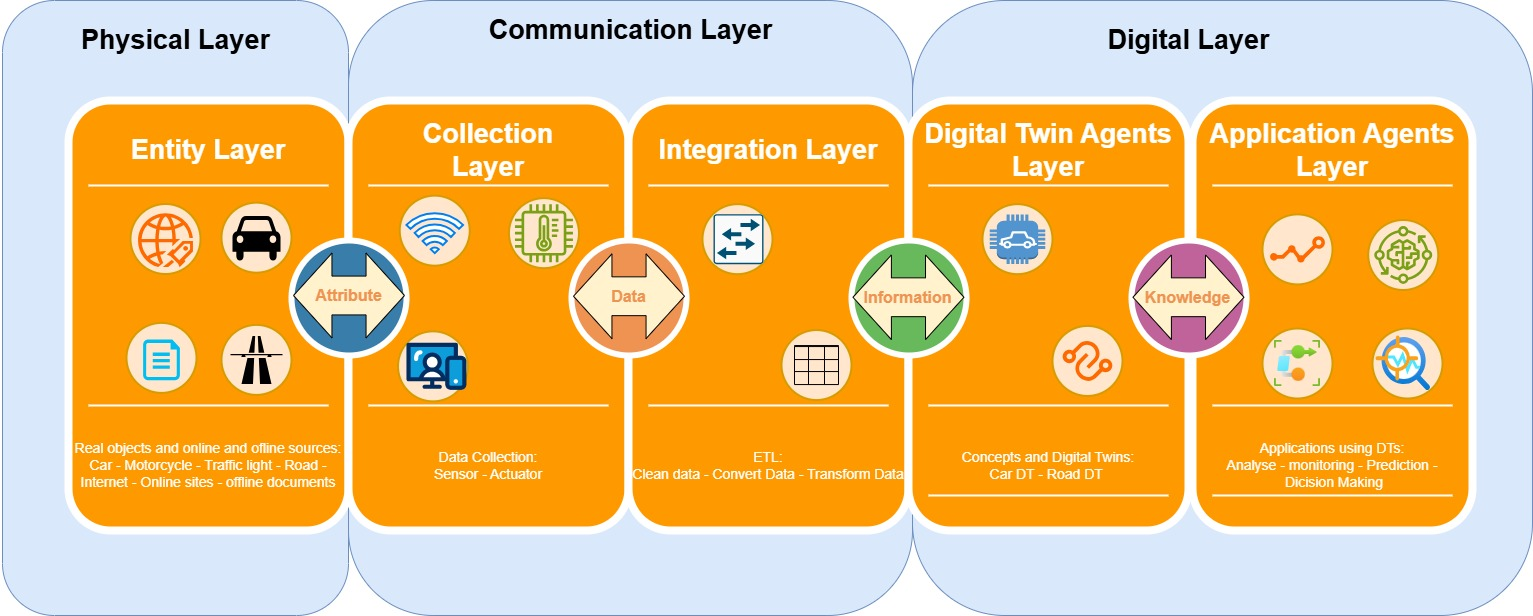
\includegraphics[width=0.98\textwidth]{images/DigitalTwin-Page-4.jpg}
    \caption{معماری پنج‌لایه پیشنهادی دوقلو‌های دیجیتال چندعاملی؛ لایه‌های موجودیت، جمع‌آوری، ادغام، عامل‌های دوقلوی دیجیتال و عامل‌های کاربرد، جریان صعودی داده و جریان نزولی فرمان و بازخورد را تشکیل می‌دهند.}
    \label{fig:arch-5layers}
\end{figure}


\subsection{لایه موجودیت}
\label{sec:layer-entity}

\gls{EmtityLayer} پایین‌ترین لایه معماری و نقطه اتصال سامانه دیجیتال به جهان فیزیکی است. این لایه شامل تجهیز یا فرآیند واقعی مورد مطالعه، حسگرها، عملگرها و سایر مؤلفه‌هایی است که وضعیت فیزیکی سیستم را تعیین می‌کنند. در چارچوب دوقلوی دیجیتال، وجود این موجودیت فیزیکی به‌تنهایی کافی نیست، بلکه باید ارتباطی پایدار میان وضعیت آن و بازنمایی دیجیتال برقرار شود تا تغییرات موجودیت واقعی بتواند در مدل دیجیتال بازتاب شود و در صورت وجود مسیر کنترلی، تصمیم‌های حاصل از فضای دیجیتال نیز به موجودیت فیزیکی منتقل شوند \cite{tao2019digital,barricelli2019survey,fuller2020digital}.
 از این دید، لایه موجودیت را می‌توان منشأ تولید داده در سامانه دانست؛ زیرا داده‌های مربوط به چرخه کاری، وضعیت حسگرها و رویدادهای عملیاتی از همین لایه وارد زنجیره پردازش می‌شوند. در کاربرد مورد نظر این پژوهش، هر موتور هواپیما به‌عنوان یک موجودیت فیزیکی مستقل در نظر گرفته می‌شود و مجموعه‌ای از متغیرها و شاخص‌های آن موجودیت در طول چرخه‌های عملیاتی ثبت می‌گردد. این ساختار با نوع داده‌های \gls{CMAPSS} نیز سازگار است؛ زیرا این مجموعه داده، توالی‌های چندمتغیره از وضعیت موتور را در چرخه‌های متوالی ارائه می‌کند و امکان مطالعه روند تخریب و برآورد \gls{RUL} را فراهم می‌سازد \cite{NASA2007C-MAPSS}.

در این لایه، مفهوم «دوقلو» نباید با صرفاً ذخیره‌سازی داده‌های شاخص‌ها اشتباه گرفته شود. مطابق ادبیات دوقلوی دیجیتال، تمایز اصلی میان یک مدل دیجیتال و یک دوقلوی دیجیتال در وجود ارتباط پویا و قابل‌اتکا میان موجودیت فیزیکی و مدل دیجیتال است به طوری که همراه با سازوکار به‌روزرسانی و تبادل اطلاعات باشد \cite{fuller2020digital,tao2019digital}. از این رو، داده‌های تولیدشده در لایه موجودیت در معماری پیشنهادی مستقیماً به‌عنوان ورودی تصمیم‌گیری در نظر گرفته نمی‌شوند، بلکه از طریق لایه جمع‌آوری و سپس لایه ادغام به یک نمایش ساختاریافته و قابل استفاده برای عامل‌های دیجیتال تبدیل می‌شوند.


\subsection{لایه جمع‌آوری داده}
\label{sec:layer-collection}

\gls{DataCollectionLayer} مسئول برقراری ارتباط عملیاتی با موجودیت فیزیکی و دریافت داده‌های خام است. وظیفه اصلی این لایه، نمونه‌برداری، دریافت، زمان‌بندی و انتقال اندازه‌گیری‌های حسگرها به لایه‌های بالاتر است و از نظر معماری نباید مسئول استنتاج یا تصمیم‌گیری باشد. این جداسازی اهمیت ویژه‌ای دارد؛ زیرا در یک سامانه چندعاملی، اگر منطق تحلیل و جمع‌آوری داده در یک عامل واحد ترکیب شود، تغییر مدل پیش‌بینی یا افزودن منبع داده جدید می‌تواند کل زنجیره پردازش را تحت تأثیر قرار دهد. چارچوب‌های  دوقلو‌های دیجیتال نیز بر اهمیت زیرساخت داده برای حفظ همگام‌سازی میان موجودیت فیزیکی و فضای دیجیتال تأکید می‌کنند \cite{qi2021enabling,fuller2020digital}.

در کاربرد حاضر، این لایه داده‌های مربوط به یک موتور را در هر چرخه کاری دریافت کرده و آن‌ها را با شناسه موجودیت، زمان یا شماره چرخه و مشخصات منبع داده برچسب‌گذاری می‌کند. در یک پیاده‌سازی واقعی، ملاحظاتی مانند نرخ نمونه‌برداری، تأخیر ارتباطی، از دست رفتن بسته‌ها، داده‌های ناقص و کشف تجهیزات جدید باید در همین لایه مدیریت شوند؛ اما در آزمایش مبتنی بر یک مجموعه داده مانند \gls{CMAPSS}، تمرکز اصلی بر شبیه‌سازی جریان داده حسگری و حفظ ترتیب زمانی نمونه‌ها است. چنین رویکردی امکان می‌دهد که معماری پیشنهادی از یک طرف با محدودیت‌های یک محیط صنعتی واقعی سازگار باشد و از طرف دیگر، در محیط آزمایشگاهی نیز به‌صورت قابل تکرار ارزیابی شود.


\subsection{لایه ادغام}
\label{sec:layer-integration}

\gls{IntegrationLayer} واسط میان جریان داده خام و فضای معنایی مورد استفاده عامل‌های دیجیتال است. داده‌های خروجی از لایه جمع‌آوری در این بخش تمیز، هنجارسازی، هم‌تراز و به قالب استاندارد تبدیل می‌شوند تا هم برای مدل پیش‌بینی و هم برای وضعیت دوقلوی دیجیتال قابل استفاده باشند. در معماری پیشنهادی، این لایه شامل چهار عملیات اصلی است: کنترل کیفیت و پاک‌سازی داده‌ها، هنجارسازی ویژگی‌ها، تشکیل پنجره‌های زمانی و ایجاد یک قرارداد داده استاندارد برای تبادل اطلاعات با عامل‌های دیجیتال. این تفکیک از اهمیت ویژه‌ای برخوردار است، زیرا مدل‌های توالی‌محور مانند LSTM به ساختار زمانی منظم و مقیاس‌بندی مناسب ویژگی‌ها حساس هستند \cite{heimes2008recurrent} و در کاربردهای  دوقلو‌های دیجیتال نیز سازگاری قالب داده و معنای سیگنال‌ها برای ایجاد یکپارچگی میان اجزای مختلف سامانه ضروری است \cite{qi2021enabling}.

در بخش پیش‌بینی \gls{RUL}، داده‌های چندمتغیره حسگرهای موتور در پنجره‌های زمانی متوالی سازمان‌دهی می‌شوند. بنابراین، اگر $x_t$ بردار اندازه‌گیری‌های حسگری موتور در چرخه $t$ باشد، یک پنجره ورودی با طول $L$ را می‌توان به‌صورت $\mathbf{X}_{t-L+1:t}=[x_{t-L+1},\ldots,x_t]$ تعریف کرد. این پنجره پس از هنجارسازی به عامل پیش‌بینی ارسال می‌شود و مدل LSTM با استفاده از وابستگی‌های زمانی موجود در توالی، مقدار $\widehat{RUL}_t$ که نشان‌دهنده مقدار عمر باقیمانده پیش‌بینی‌شده است را تولید می‌کند. استفاده از مدل‌های بازگشتی برای برآورد \gls{RUL} کاربرد فراوانی دارد و LSTM به‌دلیل توانایی در مدل‌سازی وابستگی‌های زمانی یکی از \glspl{Baseline} مهم این حوزه محسوب می‌شود \cite{heimes2008recurrent,park2026hybriddt}. بنابراین، لایه ادغام در معماری حاضر صرفاً یک مرحله پیش‌پردازش نیست، بلکه نقطه‌ای است که در آن داده خام به یک نمایش زمانی و معنایی قابل استفاده برای اجزای تحلیلی تبدیل می‌شود.

خروجی این لایه به‌صورت یک قرارداد داده ساختاریافته تعریف می‌شود که حداقل شامل شناسه موتور، شماره چرخه، بردار حسگرهای هنجارشده، پنجره زمانی ورودی، کیفیت داده و آخرین وضعیت پیش‌بینی‌شده است. وجود چنین قراردادی باعث می‌شود عامل‌های لایه دیجیتال به جزئیات نحوه دریافت داده وابسته نباشند و بتوانند اطلاعات را از منابع متفاوت، مشروط بر رعایت قرارداد، دریافت کنند. این ویژگی در معماری‌های مقیاس‌پذیر دوقلوهای دیجیتال اهمیت اساسی دارد و با تأکید پژوهش‌های جدید بر استانداردسازی در سامانه‌های دوقلوی دیجیتال هم‌راستا است \cite{park2026hybriddt,fu2026genaidt}.


\subsection{لایه عامل‌های دوقلوی دیجیتال}
\label{sec:layer-dt-agents}

\gls{DigitalTwinAgentsLayer} هسته دیجیتال معماری پیشنهادی را تشکیل می‌دهد و مسئول نگهداری وضعیت جاری هر موجودیت فیزیکی در فضای دیجیتال است. در این لایه، به ازای هر موتور یا هر موجودیت تحت پایش، یک عامل دوقلوی دیجیتال می‌تواند مسئول نگهداری وضعیت همان موجودیت باشد. این عامل لزوماً خود مدل پیش‌بینی \gls{RUL} نیست؛ بلکه به‌عنوان نماینده دیجیتال موجودیت عمل کرده و داده‌های دریافتی، نتایج پیش‌بینی، وضعیت سلامت، زمان آخرین به‌روزرسانی و سایر متغیرهای مورد نیاز را در یک ساختار وضعیت منسجم نگهداری می‌کند. چنین تفکیکی با مفهوم \gls{MA-DT} سازگار است که در آن عامل‌ها می‌توانند نماینده موجودیت‌ها یا خدمات مختلف باشند و از طریق تعامل و تبادل پیام، یک سامانه توزیع‌شده را شکل دهند \cite{pretel2022masdt,lopez2024madtwin,wang2024multiagent}.

وضعیت زنده هر عامل دوقلو را می‌توان به‌صورت یک بردار یا شیء ساختاریافته مانند رابطه \eqref{eq:digital-agent-parameter} در نظر گرفت که در آن $ID_k$ شناسه موتور، $t$ شماره چرخه جاری، $\mathbf{x}_{t-L+1:t}$ پنجره اخیر داده‌های حسگری، $\widehat{RUL}_t$ مقدار \gls{RUL} پیش‌بینی‌شده، $H_t$ وضعیت سلامت، $Q_t$ شاخص کیفیت یا اطمینان داده و $P_t$ وضعیت فعال یا غیر فعال‌بودن موتور است. در نتیجه، عامل دوقلو به جای آنکه تنها آخرین مقدار \gls{RUL} را نگه دارد، یک وضعیت دیجیتال قابل پرس‌وجو در اختیار عامل‌های کاربرد قرار می‌دهد. این موضوع اهمیت زیادی دارد، زیرا پاسخ به یک پرسش سطح‌بالا مانند «\gls{RUL} موتور $k$ چقدر است؟» ممکن است تنها به یک عدد محدود نشود و به اطلاعاتی درباره چرخه فعلی، وضعیت سلامت، آخرین به‌روزرسانی، روند تغییر \gls{RUL} و عوامل مؤثر نیز نیاز داشته باشد.

\begin{equation}\label{eq:digital-agent-parameter}
 S_k(t)=\{ID_k,t,\mathbf{x}_{t-L+1:t},\widehat{RUL}_t,H_t,Q_t,P_t\}
\end{equation}


از منظر معماری، قرار دادن این وضعیت در یک لایه مستقل باعث می‌شود که عامل‌های کاربردی مستقیماً با لایه حسگر یا مدل پیش‌بینی درگیر نشوند. به بیان دیگر، عامل کاربردی به جای آنکه بداند داده حسگر با کدام \gls{Protocol} دریافت شده یا LSTM چگونه آموزش دیده است، تنها یک رابط معنایی برای پرس‌وجوی وضعیت دوقلوی دیجیتال در اختیار دارد. این ویژگی یکی از مهم‌ترین مزایای استفاده از دوقلو‌های دیجیتال به‌عنوان واسط میان داده و کاربرد است و با معماری‌های چندعاملی دوقلوی دیجیتال که بر جداسازی مسئولیت موجودیت از خدمات کاربردی تأکید دارند، سازگار است \cite{pretel2022masdt,lopez2024madtwin,wang2024multiagent}. همچنین، با ورود مدل‌های بنیادین و عامل‌های هوشمند، دوقلوهای دیجیتال می‌توانند از یک نمایش \gls{Passive} به یک موجودیت \gls{Cognitive} و \gls{Decision-oriented} تبدیل شوند \cite{zhou2026dtai,fu2026genaidt}.


\subsection{لایه عامل‌های کاربرد}
\label{sec:layer-app-agents}

\gls{ApplicationAgentsLayer} بالاترین لایه معماری پیشنهادی و محل استقرار خدمات هوشمند و منطق تصمیم‌گیری سطح‌بالا است. برخلاف عامل‌های دوقلو که مسئول نگهداری وضعیت موجودیت هستند، عامل‌های این لایه وظیفه مشخصی را بر مبنای وضعیت موجود انجام می‌دهند. برای مثال، یک عامل می‌تواند مسئول پیش‌بینی \gls{RUL}، عامل دیگری مسئول پایش و تشخیص، عامل دیگری مسئول برنامه‌ریزی نگهداری و عامل دیگری مسئول تعامل طبیعی با کاربر باشد. این تفکیک، اصل تخصص نقش‌ها را در سامانه‌های چندعاملی محقق می‌کند و اجازه می‌دهد هر عامل با ابزار، مدل و منطق مناسب خود عمل کند \cite{dorri2018multiagent,pretel2022masdt,wang2024multiagent}.

در معماری حاضر، عامل پیش‌بینی \gls{RUL} یک مؤلفه تخصصی یادگیری ماشین است که پنجره زمانی حسگرها را دریافت و $\widehat{RUL}$ را محاسبه می‌کند. از آنجا که هدف این پژوهش برآورد عددی و قابل ارزیابی \gls{RUL} است، مسئولیت این پیش‌بینی به LSTM واگذار می‌شود و LLM در مسیر اصلی استنتاج عددی قرار نمی‌گیرد. این تصمیم معماری از نظر علمی اهمیت دارد؛ زیرا مدل‌های زبانی بزرگ در درجه نخست برای پردازش و تولید زبان، استخراج دانش، استدلال و تعامل مناسب هستند، در حالی که مدل‌های تخصصی سری زمانی برای تخمین کمّی متغیرهایی مانند \gls{RUL} مناسب‌تر و از نظر ارزیابی نیز شفاف‌تر هستند \cite{lkgstnet2026}. عامل تعامل زبانی یکی از مهم‌ترین اجزای لایه کاربرد است. وظیفه این عامل تبدیل درخواست طبیعی کاربر به یک عملیات ساختاریافته و سپس تبدیل خروجی سامانه به پاسخ قابل فهم است. در معماری‌های جدید مدل‌های زبانی بزرگ به همراه دوقلو‌های دیجیتال، مدل زبانی می‌تواند در لایه‌های مختلف از ساخت و بهره‌برداری دوقلوی دیجیتال تا ارائه خدمات و تعامل با انسان به کار گرفته شود \cite{CHEN2025102982LLMDT,zhou2026dtai}. بنابراین، در پژوهش حاضر مدل‌های زبانی بزرگ به‌عنوان یک رابط زبانی و عامل استدلالی عمل می‌کند که می‌تواند نیت کاربر را تشخیص دهد، شناسه موتور را استخراج کند، درخواست مناسب را به عامل دوقلو ارسال کند، نتایج ساختاریافته را دریافت نماید و در نهایت پاسخ توضیح‌پذیر تولید کند. پژوهش‌های جدید درباره کاربرد مدل‌های زبانی بزرگ در تولید نیز نشان می‌دهند که مدل‌های زبانی در محیط‌های صنعتی می‌توانند نقش‌هایی فراتر از تولید متن داشته باشند و در تعامل با داده‌های حسگرها، دانش سازمانی، دوقلو‌های دیجیتال و سامانه‌های چندعاملی به‌عنوان واسط استدلالی و تعاملی عمل کنند \cite{maghanaki2026llmmanufacturing}.

این لایه از نظر مقیاس‌پذیری نیز اهمیت دارد. در صورت نیاز به افزودن قابلیت جدید، می‌توان عامل جدیدی را در لایه کاربرد تعریف کرد، بدون آنکه لزوماً ساختار لایه موجودیت، جمع‌آوری یا ادغام تغییر کند. برای مثال، پس از توسعه عامل پیش‌بینی \gls{RUL} می‌توان عامل تشخیص خرابی، عامل تحلیل هزینه، عامل برنامه‌ریزی تعمیرات یا عامل ارزیابی ریسک را اضافه کرد. بنابراین، نقش عامل کاربردی در معماری حاضر تنها نمایش نتیجه \gls{RUL} نیست، بلکه تبدیل خروجی عددی مدل به دانش قابل استفاده برای تصمیم‌گیری است \cite{xagentmaint2026}.


\subsection{جریان تعامل و قرارداد ارتباطی}
\label{sec:arch-interaction}

جریان تعامل در معماری پیشنهادی از یک الگوی ارتباطی دوسویه میان لایه‌های مجاور پیروی می‌کند. جریان صعودی حامل داده، اطلاعات و دانش حاصل از موجودیت فیزیکی به سمت خدمات کاربردی است، در حالی که جریان نزولی حامل درخواست، سیاست، پارامتر، فرمان یا بازخورد است. این ویژگی باعث می‌شود معماری نه‌تنها برای پایش و پیش‌بینی، بلکه برای ایجاد یک حلقه بسته میان مشاهده، تحلیل، تصمیم و در صورت وجود زیرساخت کنترلی، اقدام نیز قابل استفاده باشد \cite{tao2019digital,qi2021enabling}. در شکل \ref{fig:arch-5layers}، این تبادل در چهار سطح مفهومی \lr{Attribute}، \lr{Data}، \lr{Information} و \lr{Knowledge} قابل مشاهده است. در مرز موجودیت و جمع‌آوری، ویژگی‌ها و اندازه‌گیری‌های فیزیکی منتقل می‌شوند؛ در مرز جمع‌آوری و ادغام، داده خام به‌صورت جریان داده منتقل می‌شود؛ در مرز ادغام و عامل دوقلوی دیجیتال، داده پردازش‌شده به اطلاعات ساختاریافته تبدیل می‌شود؛ و در مرز عامل دوقلو و عامل کاربرد، اطلاعات وضعیت به دانش و خدمات قابل استفاده برای تصمیم‌گیری تبدیل می‌شود. این تفکیک مفهومی با روند تکامل دوقلو‌های دیجیتال از جمع‌آوری داده به سمت تحلیل، پیش‌بینی و تصمیم‌گیری هوشمند سازگار است \cite{fuller2020digital,zhou2026dtai,fu2026genaidt}.

قرارداد ارتباطی میان این لایه‌ها باید علاوه بر محتوای پیام، شناسه موجودیت، زمان یا چرخه، نوع درخواست، نسخه وضعیت، کیفیت داده و منبع تولید اطلاعات را نیز مشخص کند. برای مثال، پیام خروجی لایه ادغام برای موتور $k$ می‌تواند شامل شناسه موتور، شماره چرخه، پنجره حسگر، وضعیت کیفیت داده و آخرین $\widehat{RUL}$ باشد. عامل دوقلو این پیام را دریافت کرده و وضعیت $S_k(t)$ را به‌روزرسانی می‌کند. سپس عامل کاربردی، بسته به نوع خدمت، می‌تواند تنها بخشی از این وضعیت را درخواست کند. چنین قرارداد ساختاریافته‌ای از وابستگی مستقیم عامل‌ها به ساختار داخلی یکدیگر جلوگیری کرده و زمینه را برای جایگزینی مدل مورد استفاده، اضافه کردن مدل‌های جدید یا تغییر پیاده‌سازی عامل زبانی بدون بازطراحی کل سامانه فراهم می‌کند \cite{park2026hybriddt}.

در این معماری، یک نکته مهم تفکیک میان «پیش‌بینی» و «تفسیر» است. عامل پیش‌بینی، مقدار عددی \gls{RUL} و در صورت طراحی مدل، شاخص‌هایی نظیر اهمیت ویژگی‌ها یا عدم‌قطعیت پیش‌بینی را تولید می‌کند؛ عامل دوقلوی دیجیتال این خروجی را با وضعیت جاری موتور ترکیب و ذخیره می‌کند؛ و عامل زبانی از این وضعیت ساختاریافته برای تولید پاسخ انسانی استفاده می‌نماید. بنابراین، مدل زبانی بزرگ نباید بدون دسترسی به وضعیت معتبر دوقلو یا داده‌های ساختاریافته، مقدار \gls{RUL} را از خود تولید کند. این طراحی خطر ایجاد پاسخ‌های زبانی غیرمستند را کاهش داده و نقش مدل زبانی بزرگ را به حوزه‌ای محدود می‌کند که در آن بیشترین ارزش افزوده را دارد: تفسیر، ترکیب دانش، تعامل و هدایت جریان کار \cite{zhou2026dtai}.


\subsection{فرایند تعامل کاربر، عامل زبانی و عامل پیش‌بینی عمر مفید باقیمانده}
\label{sec:arch-sequence}

شکل \ref{fig:arch-sequence} نمونه‌ای از اجرای عملی معماری پیشنهادی را برای پرسش «\gls{RUL} موتور $k$ چیست؟» نشان می‌دهد. این فرایند عمداً به‌گونه‌ای طراحی شده است که تعامل طبیعی کاربر با سامانه از منطق داخلی پیش‌بینی جدا باقی بماند. در این فرایند، کاربر مستقیماً با مدل LSTM یا پایگاه داده حسگرها ارتباط ندارد؛ بلکه درخواست خود را از طریق عامل تعامل زبانی مطرح می‌کند. عامل زبانی پس از تشخیص نیت و استخراج شناسه موتور، یک درخواست ساختاریافته برای عامل دوقلوی دیجیتال ایجاد می‌کند. عامل دوقلو با توجه به وضعیت جاری موتور، پنجره زمانی مورد نیاز را از لایه ادغام دریافت کرده و آن را به عامل پیش‌بینی \gls{RUL} ارسال می‌کند. عامل پیش‌بینی پس از اجرای مدل، مقدار $\widehat{RUL}$ و در صورت پشتیبانی مدل، شاخص اهمیت حسگرها یا سایر شواهد پیش‌بینی را بازمی‌گرداند. عامل دوقلو سپس وضعیت دیجیتال موتور را به‌روزرسانی کرده و یک نمایش ساختاریافته از وضعیت را در اختیار عامل زبانی قرار می‌دهد. در مرحله نهایی، عامل زبانی این اطلاعات را به پاسخ طبیعی و توضیح‌پذیر برای کاربر تبدیل می‌کند. این معماری با رویکردهای جدیدی که مدل‌های زبانی را در لایه تعامل و سرویس دوقلو‌های دیجیتال قرار می‌دهند و در عین حال مدل‌های تخصصی را برای وظایف تحلیلی حفظ می‌کنند، سازگار است \cite{CHEN2025102982LLMDT,maghanaki2026llmmanufacturing,zhou2026dtai}.

\begin{figure}[H]
    \centering
    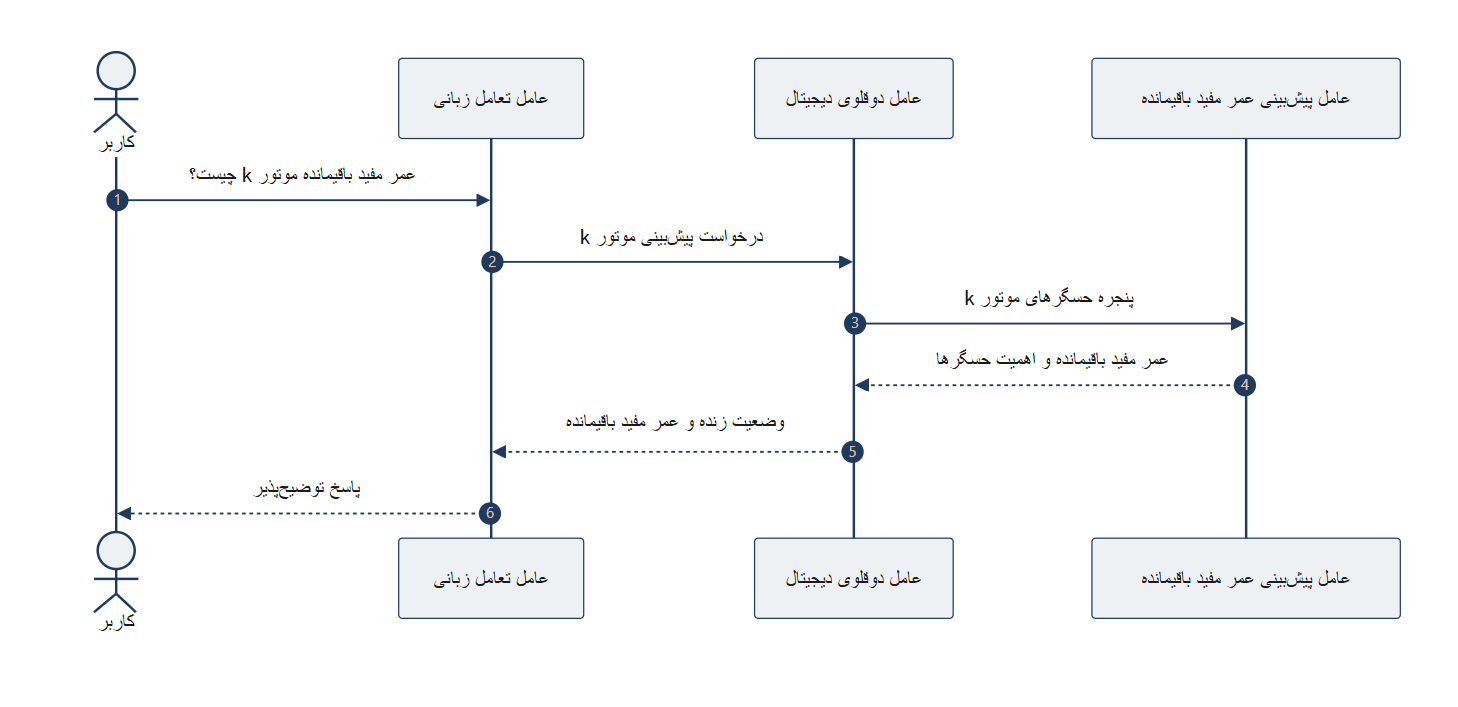
\includegraphics[width=1.1\textwidth]{images/arch_sequence4.png}
    \caption{
    	دیاگرام توالی تعامل برای پاسخ‌گویی به پرسش «عمر مفید باقیمانده موتور $k$ چیست؟»؛ درخواست از کاربر به عامل زبانی و سپس به عامل دوقلو و عامل پیش‌بینی منتقل می‌شود و نتیجه پس از به‌روزرسانی وضعیت دوقلو، به‌صورت پاسخ توضیح‌پذیر به کاربر بازمی‌گردد.}
    \label{fig:arch-sequence}
\end{figure}

مطابق شکل \ref{fig:arch-sequence}، نخست کاربر پرسش خود را از طریق رابط زبانی ارسال می‌کند. در گام دوم، عامل تعامل زبانی نیت کاربر را شناسایی کرده و شناسه $k$ را از عبارت ورودی استخراج می‌کند. در گام سوم، عامل دوقلوی دیجیتال درخواست مربوط به موتور $k$ را دریافت کرده و پنجره زمانی مورد نیاز برای پیش‌بینی را از لایه ادغام دریافت می‌کند؛ این پنجره شامل توالی آخرین اندازه‌گیری‌های حسگری مورد نیاز مدل \gls{RUL} است. در گام چهارم، عامل پیش‌بینی \gls{RUL} این توالی را به مدل تخصصی ارسال کرده و $\widehat{RUL}_k(t)$ را محاسبه می‌کند. در صورت استفاده از یک روش توضیح‌پذیر، اطلاعاتی مانند اهمیت نسبی حسگرها نیز در همین مرحله تولید می‌شود. در گام پنجم، نتیجه پیش‌بینی به عامل دوقلو بازگردانده شده و عامل دوقلو وضعیت زنده موتور را با مقدار جدید \gls{RUL} و سایر اطلاعات همراه به‌روزرسانی می‌کند. در گام ششم، عامل تعامل زبانی وضعیت ساختاریافته را دریافت کرده و پاسخ نهایی را تولید می‌کند؛ برای مثال، پاسخ می‌تواند شامل مقدار \gls{RUL}، وضعیت فعلی موتور، چرخه جاری، سطح هشدار و مهم‌ترین عوامل مؤثر بر پیش‌بینی باشد.

این توالی نشان می‌دهد که معماری پیشنهادی در واقع یک زنجیره ساده ``مدل‌های زبانی بزرگ $\rightarrow$ \gls{RUL}'' نیست، بلکه یک حلقه ``کاربر $\rightarrow$ مدل زبانی بزرگ $\rightarrow$ عامل دوقلوی دیجیتال $\rightarrow$ عامل \gls{RUL} $\rightarrow$ عامل دوقلوی دیجیتال $\rightarrow$ مدل زبانی بزرگ $\rightarrow$ کاربر'' است. این تمایز از منظر طراحی سامانه اهمیت دارد، زیرا دوقلو‌های دیجیتال در اینجا نقش حافظه وضعیت و واسط معنایی میان مدل‌های تخصصی و عامل‌های کاربردی را ایفا می‌کند. از سوی دیگر، مدل‌ زبانی بزرگ وظیفه تولید یا جعل وضعیت فیزیکی را ندارد، بلکه فقط بر اساس وضعیت بازیابی‌شده از دوقلوی دیجیتال، پاسخ و توضیح تولید می‌کند \cite{zhou2026dtai,fu2026genaidt}.

از دیدگاه نگهداری پیش‌بینانه، این معماری امکان گسترش فرایند پرسش و پاسخ ساده به فرآیندهای تصمیم‌گیری پیچیده‌تر را نیز فراهم می‌کند. برای مثال، پس از دریافت وضعیت موتور، یک عامل تشخیص می‌تواند علت احتمالی افت سلامت را بررسی کند، یک عامل برنامه‌ریزی می‌تواند زمان مناسب نگهداری را پیشنهاد دهد، یک عامل هزینه می‌تواند هزینه توقف و تعمیر را محاسبه کند و در نهایت عامل زبان طبیعی می‌تواند خروجی این عامل‌ها را برای کاربر ترکیب کند. چنین توسعه‌ای با روند اخیر حرکت از دوقلو‌های دیجیتال منفرد به دوقلو‌های دیجیتال چندعاملی و \glspl{Agentic Digital Twin}  سازگار است \cite{coulibaly2026madtdt}. در نتیجه، معماری حاضر می‌تواند به‌عنوان یک زیرساخت قابل توسعه برای حرکت از ``پیش‌بینی \gls{RUL}'' به \gls{Agentic Predictive Maintenance} مورد استفاده قرار گیرد.

بر این اساس، معماری پیشنهادی را می‌توان به‌صورت یک زنجیره لایه‌ای و در عین حال دوسویه تعریف کرد که در آن داده از موجودیت فیزیکی به سمت دانش و تصمیم حرکت می‌کند و فرمان یا درخواست در مسیر معکوس به سمت موجودیت بازمی‌گردد. این ساختار علاوه بر حفظ استقلال مدل‌های تخصصی، امکان افزودن مدل‌های زبانی بزرگ، عامل‌های جدید، روش‌های پیشرفته‌تر پیش‌بینی مانند \glspl{Transformer} و سازوکارهای تصمیم‌گیری چندعاملی را فراهم می‌سازد. از این منظر، ارزش اصلی معماری پیشنهادی در یک مدل یادگیری منفرد خلاصه نمی‌شود، بلکه در ایجاد یک چارچوب یکپارچه برای اتصال داده‌های حسگری، پیش‌بینی \gls{RUL}، وضعیت دوقلو‌های دیجیتال، استدلال زبانی و همکاری عامل‌ها است. چارچوبی که می‌تواند در مراحل بعدی پژوهش به سمت تصمیم‌گیری خودکار، برنامه‌ریزی نگهداری و حلقه بسته انسان--عامل--دوقلوی‌ دیجیتال توسعه یابد.

%------------------------------------------------------------------------

% -----------------------------------------------------------------------
\section{مجموعه داده \lr{CMAPSS} و آماده‌سازی داده}
\label{sec:dataset}

\subsection{معرفی و ساختار مجموعه داده}
\label{sec:dataset-intro}

برای ارزیابی تجربی معماری پیشنهادی، از مجموعه داده
\gls{CMAPSS} استفاده شده است. این مجموعه داده توسط مرکز پژوهشی
\lr{NASA Ames Research Center}
تولید شده و یکی از مجموعه داده‌های مرجع در پژوهش‌های مرتبط با
پیش‌بینی \gls{RUL} موتورهای جت به شمار
می‌رود \cite{NASA2007C-MAPSS}.
در این شبیه‌سازی، وضعیت موتور در چرخه‌های کاری متوالی ثبت می‌شود و
داده‌های حسگری حاصل از روند تخریب موتور، امکان توسعه و مقایسه
روش‌های مختلف پیش‌آگاهی و پیش‌بینی \gls{RUL} را فراهم می‌کند.

اهمیت \gls{CMAPSS} برای پژوهش حاضر از ماهیت چندمتغیره و زمانی داده‌ها
ناشی می‌شود. هر موتور به‌صورت یک دنباله زمانی مستقل مشاهده می‌شود و
مقادیر حسگرها در طول چرخه‌های متوالی تغییر می‌کنند. بنابراین، مسئله
تنها یک مسئله رگرسیون ایستا نیست، بلکه پیش‌بینی \gls{RUL} مستلزم
استخراج اطلاعات مرتبط با روند تغییرات وضعیت موتور، در طول زمان است.
به همین دلیل، این مجموعه داده از نخستین سنجه‌های مهم برای بررسی
روش‌های مبتنی بر شبکه‌های بازگشتی و همچنین روش‌های یادگیری عمیق در
پیش‌بینی \gls{RUL} بوده است \cite{heimes2008recurrent}.
همچنین، مطالعات بر روی مجموعه داده CMAPSS نشان داده‌اند که
تفاوت در شرایط عملیاتی، تعداد حالت‌های خرابی، نویز حسگرها و نحوه
پردازش داده می‌تواند تأثیر قابل‌توجهی بر مقایسه منصفانه مدل‌های
پیش‌بینی داشته باشد \cite{NASA2007C-MAPSS}.

مجموعه داده \gls{CMAPSS} از چهار زیرمجموعه
\lr{FD001} تا \lr{FD004} تشکیل شده است. این زیرمجموعه‌ها از نظر
تعداد شرایط عملیاتی و حالت‌های خرابی با یکدیگر تفاوت دارند. در
\lr{FD001} تنها یک شرایط عملیاتی و یک حالت خرابی در نظر گرفته شده
است؛ \lr{FD002} شامل شش شرایط عملیاتی و یک حالت خرابی است؛
\lr{FD003} شامل یک شرایط عملیاتی و دو حالت خرابی است؛ و
\lr{FD004} شامل شش شرایط عملیاتی و دو حالت خرابی است
\cite{NASA2007C-MAPSS}. از این منظر،
\lr{FD001} ساده‌ترین فرایند این مجموعه داده محسوب می‌شود و
\lr{FD004} پیچیده‌ترین ترکیب شرایط عملیاتی و حالت‌های خرابی را
ارائه می‌کند.

مشخصات چهار زیرمجموعه در جدول
\ref{tab:cmapss-subsets} ارائه شده است. در پژوهش حاضر، \lr{FD001}
به‌عنوان فرایند اصلی آزمایش انتخاب شده است. این انتخاب به معنای
برتری ذاتی \lr{FD001} نسبت به سایر زیرمجموعه‌ها نیست، بلکه با هدف
ایجاد یک سناریوی کنترل‌شده برای ارزیابی اولیه معماری انجام شده است.
از آنجا که در این زیرمجموعه تغییر شرایط عملیاتی و تنوع حالت خرابی
نسبت به \lr{FD002} و \lr{FD004} محدودتر است، می‌توان اثر معماری
پیشنهادی و مدل پیش‌بینی را با پیچیدگی کمتری بررسی کرد
\cite{NASA2007C-MAPSS}. ارزیابی زیرمجموعه‌های پیچیده‌تر می‌تواند
در ادامه به‌عنوان توسعه آزمایش‌ها انجام شود.

\begin{table}[ht]
	\centering
	\caption{مشخصات زیرمجموعه‌های مجموعه داده \lr{CMAPSS}}
	\label{tab:cmapss-subsets}
	\begin{tabular}{ccccc}
		\toprule
		\textbf{زیرمجموعه} &
		\textbf{شرایط عملیاتی} &
		\textbf{حالت خرابی} &
		\textbf{موتور آموزش} &
		\textbf{موتور آزمون} \\
		\midrule
		\lr{FD001} & ۱ & ۱ & ۱۰۰ & ۱۰۰ \\
		\lr{FD002} & ۶ & ۱ & ۲۶۰ & ۲۵۹ \\
		\lr{FD003} & ۱ & ۲ & ۱۰۰ & ۱۰۰ \\
		\lr{FD004} & ۶ & ۲ & ۲۴۸ & ۲۴۸ \\
		\bottomrule
	\end{tabular}
\end{table}

در سطح رکورد، داده خام \gls{CMAPSS} شامل ۲۶ ستون است که از شناسه
موتور، شماره چرخه کاری، سه متغیر تنظیم عملیاتی و ۲۱ متغیر حسگری
تشکیل می‌شود. شناسه موتور با \lr{unit\_number} مشخص شده و برای
تفکیک تاریخچه موتورهای مختلف به‌کار می‌رود. متغیر
\lr{time\_in\_cycles} نیز موقعیت مشاهده در چرخه عمر موتور را نشان
می‌دهد. سه متغیر تنظیم عملیاتی شرایط کاری شبیه‌سازی‌شده را توصیف
می‌کنند و ۲۱ حسگر اطلاعات مرتبط با وضعیت عملیاتی و سلامت موتور را
ثبت می‌کنند \cite{NASA2007C-MAPSS}.

از دیدگاه یادگیری ماشین، داده هر موتور را می‌توان به‌صورت یک سری
زمانی چندمتغیره نمایش داد. اگر $x_t \in \mathbb{R}^{d}$ بردار
ویژگی‌های موتور در چرخه $t$ باشد، تاریخچه موتور به‌صورت دنباله‌ای
از بردارهای
$\{\mathbf{x}_1,\mathbf{x}_2,\ldots,\mathbf{x}_T\}$
در نظر گرفته می‌شود. این ساختار امکان استفاده از مدل‌های توالی‌محور
مانند \gls{LSTM} را فراهم می‌کند؛ زیرا چنین مدل‌هایی می‌توانند
اطلاعات چند گام زمانی متوالی را در فرآیند برآورد \gls{RUL} لحاظ
کنند \cite{heimes2008recurrent}.

در آزمایش اصلی این پژوهش، فایل آموزش \lr{train\_FD001.txt}
شامل ۲۰۶۳۱ مشاهده مربوط به ۱۰۰ موتور است و تاریخچه هر موتور تا
چرخه خرابی در دسترس قرار دارد. فایل
\lr{test\_FD001.txt} نیز شامل ۱۳۰۹۶ مشاهده مربوط به ۱۰۰ موتور است؛
با این تفاوت که تاریخچه موتورهای آزمون پیش از خرابی متوقف شده است.
بنابراین، زمان واقعی خرابی موتورهای آزمون مستقیماً در فایل آزمون
مشاهده نمی‌شود و برای محاسبه مقدار واقعی \gls{RUL} باید از فایل
\lr{RUL\_FD001.txt} استفاده شود. این ساختار، مسئله آزمون را به
فرایندی نزدیک می‌کند که در آن وضعیت فعلی تجهیز مشاهده می‌شود اما
زمان خرابی آینده هنوز رخ نداده است \cite{NASA2007C-MAPSS}.

\subsection{تحلیل اکتشافی و انتخاب ویژگی}
\label{sec:eda}

پیش از تشکیل ورودی مدل، داده آموزشی از نظر تغییرپذیری ویژگی‌ها،
ارتباط با متغیر هدف و تغییرات مقادیر حسگر‌ها بررسی شد. هدف از
این مرحله کاهش ویژگی‌هایی است که یا فاقد اطلاعات تغییرپذیر هستند،
یا اطلاعات تکراری ارائه می‌کنند، یا در چارچوب آزمایش حاضر، ارزش
پیش‌بینی محدودی دارند. استفاده از چنین مرحله‌ای با رویه‌های رایج
در مطالعات \gls{CMAPSS} سازگار است. با این حال، مجموعه ویژگی نهایی باید
بر اساس داده و \gls{Protocol} همان پژوهش تعیین شود، زیرا انتخاب ویژگی در
مطالعات مختلف \gls{CMAPSS} یکسان نیست \cite{smith2025cmapsslinear,li2025attentiondt}.

در پژوهش حاضر، ابتدا ویژگی‌های فاقد تغییرپذیری مؤثر در داده
آموزشی شناسایی و حذف شدند. علاوه بر آن، همبستگی میان متغیرهای
حسگرها و \gls{RUL} بررسی شد تا متغیرهایی که در فرایند
\lr{FD001}
 اطلاعات محدودی ارائه می‌کنند مشخص شوند. در این مرحله،
ضریب همبستگی \lr{Pearson} به‌عنوان یک معیار توصیفی مورد استفاده
قرار گرفت. لازم به تأکید است که مقدار همبستگی به‌تنهایی مبنای
کافی برای حذف یک حسگر نیست؛ زیرا رابطه یک حسگر با \gls{RUL}
ممکن است غیرخطی یا وابسته به تاریخچه زمانی باشد. ازاین‌رو،
نتایج همبستگی در این پژوهش به‌عنوان ابزار تحلیل اکتشافی و نه یک
آزمون قطعی اهمیت ویژگی تفسیر شده‌اند.


پس از محاسبه برچسب \gls{RUL}، ضریب همبستگی \lr{Pearson} میان ویژگی‌های باقیمانده و متغیر هدف محاسبه شد. همان‌گونه که در شکل \ref{fig:corr-heatmap} مشاهده می‌شود، \gls{RUL} با \lr{time\_in\_cycles}، \lr{Ps30}، \lr{T50} و \lr{BPR} رابطه منفی نسبتاً قوی دارد؛ به این معنا که با افزایش چرخه‌های کاری و نزدیک شدن موتور به انتهای عمر، مقدار عمر مفید باقیمانده کاهش می‌یابد. در مقابل، ویژگی‌هایی نظیر \lr{phi}، \lr{W31} و \lr{W32} رابطه مثبت قابل‌توجهی با \gls{RUL} نشان می‌دهند. همچنین، دو متغیر \lr{setting\_1} و \lr{setting\_2} رابطه بسیار ضعیفی با متغیر هدف دارند و \lr{P15} نیز ارتباط محدودی نشان می‌دهد. نکته مهم دیگر، همبستگی بسیار بالای میان \lr{Nc} و \lr{NRc} با مقدار تقریبی $0.96$ است که نشان می‌دهد نگه‌داری هم‌زمان این دو متغیر می‌تواند اطلاعات تکراری وارد مدل کند. از این رو، انتخاب ویژگی در پژوهش حاضر صرفاً بر مبنای مقدار همبستگی با \gls{RUL} انجام نشده، بلکه ترکیبی از حذف ویژگی‌های ثابت، حذف ویژگی‌های کم‌اطلاع و کاهش هم‌خطی میان متغیرهای حسگری مورد توجه قرار گرفته است.


\begin{figure}[H]
	 \centering
	  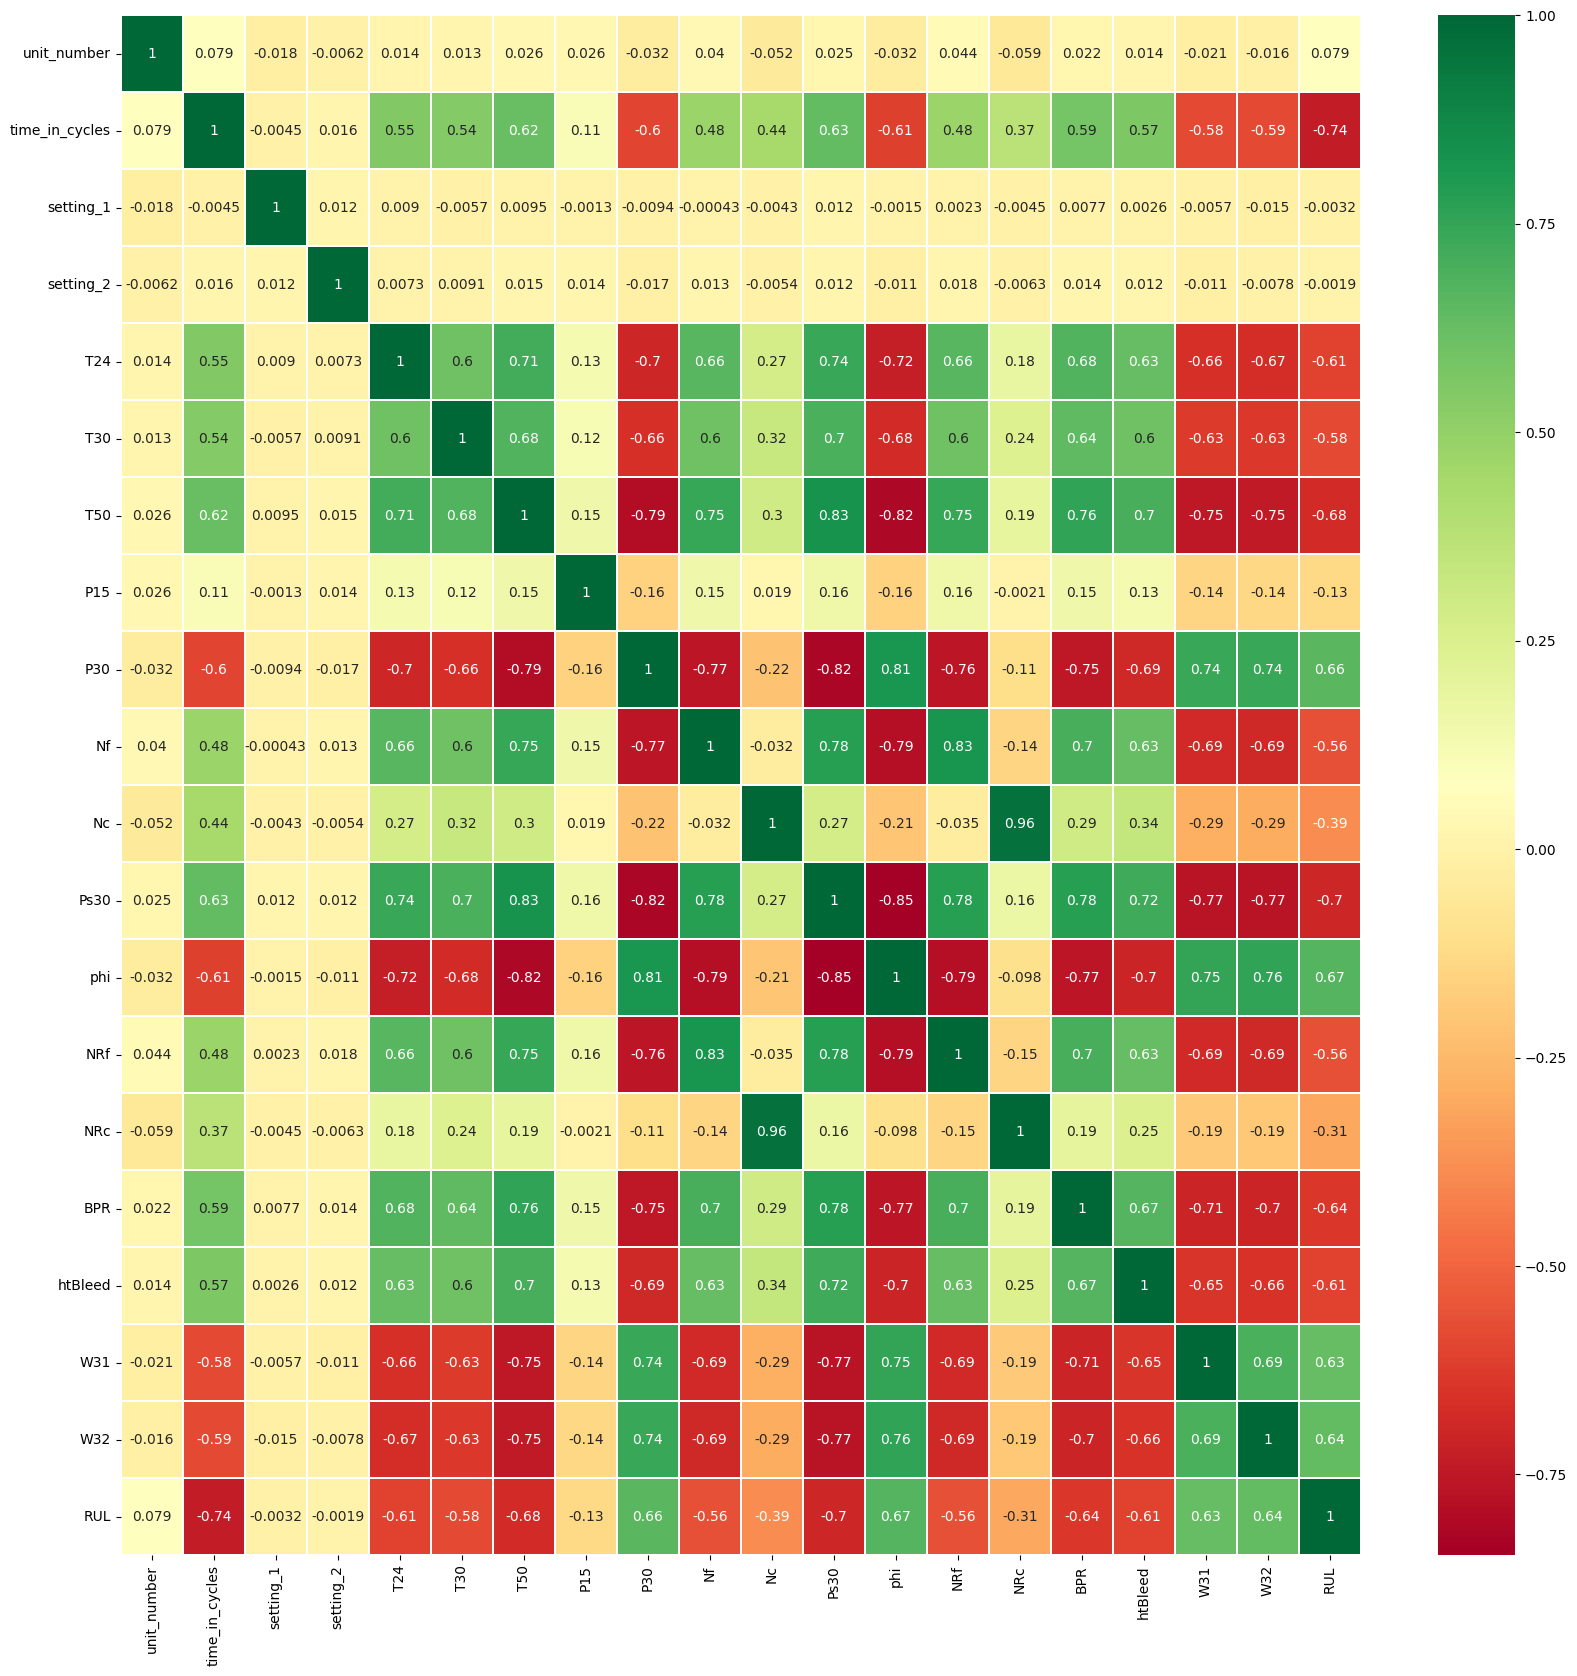
\includegraphics[width=0.98\textwidth] {images/cmapss_corr_heatmap.png}
	   \caption{نقشه همبستگی \lr{Pearson} ویژگی‌ها و برچسب عمر مفید باقیمانده در داده آموزشی \lr{FD001} پس از حذف ستون‌های ثابت} 
	   \label{fig:corr-heatmap} 
\end{figure}


بر اساس تحلیل انجام‌شده در پژوهش حاضر، ویژگی‌های
\lr{TRA}، \lr{T2}، \lr{P2}، \lr{epr}، \lr{farB}،
\lr{Nf\_dmd} و \lr{PCNfR\_dmd}
به دلیل داشتن مقدار ثابت و عدم ارائه اطلاعات مفید برای پیش‌بینی، از مجموعه ورودی حذف شدند.
همچنین \lr{setting\_1} و \lr{setting\_2} به دلیل اطلاعات محدود در
فرایند \lr{FD001} و \lr{P15} به دلیل ارزش پیش‌بینی پایین در
تحلیل حاضر کنار گذاشته شدند. افزون بر آن، به دلیل هم‌خطی شدید
میان \lr{Nc} و \lr{NRc}، تنها \lr{Nc} حفظ شد. چنین تصمیمی با
مشاهدات مطالعات پیشین درباره وجود ویژگی‌های کم‌اطلاع یا بسیار
هم‌بسته در داده‌های CMAPSS هم‌راستا است
\cite{smith2025cmapsslinear,li2025attentiondt}.

در نهایت، ۱۳ حسگر شامل
\lr{T24}، \lr{T30}، \lr{T50}، \lr{P30}، \lr{Nf}،
\lr{Nc}، \lr{Ps30}، \lr{phi}، \lr{NRf}، \lr{BPR}،
\lr{htBleed}، \lr{W31} و \lr{W32}
برای استفاده در مدل انتخاب شدند. علاوه بر این، شماره چرخه به‌صورت
هنجارشده با نام \lr{cycle\_norm} ایجاد شد تا موقعیت نسبی موتور در
طول عمر مشاهده‌شده آن به مدل ارائه شود. در جدول
 \ref{tab:feature-selection}
 مراحل انتخاب ویژگی به صورت خلاصه نشان داده می‌شود.


\begin{table}[ht]
	\centering
	\caption{فرایند انتخاب ویژگی در زیرمجموعه \lr{FD001}}
	\label{tab:feature-selection}
	\begin{tabular}{p{3.8cm}p{8.8cm}}
		\toprule
		\textbf{مرحله} & \textbf{ویژگی‌ها / تصمیم} \\
		\midrule
		حذف ویژگی‌های فاقد تغییرپذیری مؤثر &
		\lr{TRA}، \lr{T2}، \lr{P2}، \lr{epr}،
		\lr{farB}، \lr{Nf\_dmd} و \lr{PCNfR\_dmd} \\
		\addlinespace
		حذف ویژگی‌های کم‌اطلاع &
		\lr{setting\_1}، \lr{setting\_2} و \lr{P15} \\
		\addlinespace
		کاهش هم‌خطی &
		حذف \lr{NRc} و حفظ \lr{Nc} \\
		\addlinespace
		حسگرهای نهایی &
		\lr{T24}، \lr{T30}، \lr{T50}، \lr{P30}، \lr{Nf}،
		\lr{Nc}، \lr{Ps30}، \lr{phi}، \lr{NRf}،
		\lr{BPR}، \lr{htBleed}، \lr{W31} و \lr{W32} \\
		\bottomrule
	\end{tabular}
\end{table}

\subsection{پیش‌پردازش و تشکیل دنباله‌های زمانی}
\label{sec:preprocessing}

پس از پاک‌سازی و انتخاب ویژگی، داده‌ها برای استفاده در مدل
توالی‌محور به نمونه‌های زمانی با طول ثابت تبدیل شدند. نخستین
مرحله، محاسبه برچسب \gls{RUL} برای داده آموزشی است. از آنجا که
تاریخچه موتورهای آموزشی تا خرابی در دسترس است، اگر
$t_{\mathrm{end}}^{(i)}$ آخرین چرخه مشاهده‌شده برای موتور $i$
باشد، مقدار واقعی \gls{RUL} در چرخه $t$ از رابطه \ref{eq:rul-label} محاسبه می‌شود:

\begin{equation}
	\label{eq:rul-label}
	y^{(i)}(t)
	=
	t_{\mathrm{end}}^{(i)}-t.
\end{equation}

در نتیجه، مقدار \gls{RUL} در آخرین چرخه موتور برابر صفر است و
برای چرخه‌های قبل، متناسب با فاصله زمانی تا خرابی افزایش می‌یابد.
این تعریف با مسائل رایج 
\gls{RUL}
در داده‌های
\gls{run-to-failure}
 سازگار است \cite{NASA2007C-MAPSS,heimes2008recurrent}.


برای داده آزمون، دنباله هر موتور پیش از وقوع خرابی قطع شده است.
بنابراین، برخلاف داده آموزشی، لحظه خرابی در فایل آزمون مشاهده نمی‌شود.
فایل \lr{RUL\_FD001.txt} تنها مقدار \gls{RUL} را در آخرین چرخه
مشاهده‌شده هر موتور ارائه می‌دهد.
اگر $t_{\mathrm{last}}^{(i)}$ آخرین چرخه مشاهده‌شده موتور $i$
و $r_{\mathrm{file}}^{(i)}$ مقدار ثبت‌شده در این فایل باشد،
لحظه خرابی به‌صورت
$t_{\mathrm{fail}}^{(i)}=t_{\mathrm{last}}^{(i)}+r_{\mathrm{file}}^{(i)}$
بازسازی می‌شود.
سپس برچسب همه چرخه‌های همان موتور، مشابه رابطه~\eqref{eq:rul-label}،
از فاصله تا لحظه خرابی به‌دست می‌آید:

\begin{equation}
	\label{eq:rul-test}
	y^{(i)}(t)
	=
	t_{\mathrm{last}}^{(i)}
	+
	r_{\mathrm{file}}^{(i)}
	-
	t
	=
	t_{\mathrm{fail}}^{(i)}-t.
\end{equation}

در نتیجه، در آخرین چرخه مشاهده‌شده داریم
$y^{(i)}\bigl(t_{\mathrm{last}}^{(i)}\bigr)=r_{\mathrm{file}}^{(i)}$
و برچسب با مقدار مرجع ناسا یکی است.
ارزیابی کمی مدل نیز روی همین نقطه، یعنی آخرین پنجره زمانی هر موتور
آزمون، انجام می‌شود.

در مرحله بعد، ویژگی‌های حسگری منتخب با استفاده از تبدیل
\lr{Min-Max} به بازه $[0,1]$ منتقل شدند:

\begin{equation}
	\label{eq:normalization}
	x_{\mathrm{norm}}
	=
	\frac{x-x_{\min}}
	{x_{\max}-x_{\min}}.
\end{equation}

برای جلوگیری از نشت اطلاعات، پارامترهای $x_{\min}$ و $x_{\max}$
تنها از داده آموزشی محاسبه شدند و همان مقادیر برای تبدیل داده
آزمون مورد استفاده قرار گرفتند. بنابراین، هیچ اطلاعاتی از توزیع
داده آزمون برای تعیین پارامترهای پیش‌پردازش وارد مرحله آموزش
نمی‌شود.


در کنار ویژگی‌های حسگرها، متغیر \lr{cycle\_norm} نیز به‌عنوان
زمان نسبی هر موتور ایجاد شد و توالی داده را مشخص کرد. همچنین با استفاده از این متغیر می‌توان گذشت زمان را در دوقلوی دیجیتال شبیه‌سازی کرد. شناسه موتور و شماره چرخه خام برای مدیریت دنباله و نگهداری وضعیت موجودیت حفظ شدند. با این حال، همان‌گونه که در بخش انتخاب ویژگی توضیح داده شد،
شناسه موتور نباید بدون توجیه روش‌شناختی به‌عنوان یک متغیر فیزیکی
سلامت تفسیر شود.

پس از هنجارسازی، از یک پنجره لغزنده با طول
$w=50$ برای تبدیل داده‌های جدولی به نمونه‌های توالی استفاده شد.
اگر $\mathbf{x}_t$ بردار ویژگی موتور در چرخه $t$ باشد، ورودی مدل
در زمان $t$ به‌صورت 
\ref{eq:lstm-window}
 تعریف می‌شود.

\begin{equation}
	\label{eq:lstm-window}
	\mathbf{X}_{t-49:t}
	=
	[
	\mathbf{x}_{t-49},
	\mathbf{x}_{t-48},
	\ldots,
	\mathbf{x}_{t}
	].
\end{equation}

در نتیجه، هر نمونه ورودی دارای ۵۰ گام زمانی متوالی است. انتخاب
پنجره زمانی به مدل اجازه می‌دهد به‌جای اتکا به یک مشاهده منفرد،
الگوی تغییرات اخیر وضعیت موتور را در پیش‌بینی \gls{RUL} لحاظ کند.
این رویکرد با ماهیت مدل‌های بازگشتی و مطالعات استفاده از LSTM برای
پیش‌بینی \gls{RUL} سازگار است \cite{heimes2008recurrent}.

برچسب هر پنجره برابر با مقدار \gls{RUL} در آخرین چرخه همان پنجره
در نظر گرفته می‌شود. بنابراین، اگر پنجره مربوط به چرخه‌های
$t-49$ تا $t$ باشد، هدف آن $y(t)$ خواهد بود. در نتیجه، هر نمونه
آموزشی اطلاعات تاریخی لازم برای تخمین عمر باقیمانده در انتهای
پنجره را در اختیار مدل قرار می‌دهد.

در نهایت، تفکیک آموزش و آزمون در سطح موتور حفظ شد و هیچ تقسیم
تصادفی از پنجره‌های زمانی انجام نشد. این تصمیم از اهمیت
روش‌شناختی بالایی برخوردار است؛ زیرا پنجره‌های متوالی یک موتور
دارای هم‌پوشانی زمانی زیادی هستند و تقسیم تصادفی آن‌ها میان
آموزش و آزمون می‌تواند موجب انتقال اطلاعات بسیار مشابه میان دو
مجموعه و در نتیجه برآورد خوش‌بینانه عملکرد مدل شود. حفظ \gls{Protocol}
اصلی \gls{CMAPSS} و تفکیک موتورهای آموزش و آزمون، امکان مقایسه منصفانه‌تر
با مطالعات پیشین را فراهم می‌کند \cite{NASA2007C-MAPSS}.


% =======================================================================

% انطباق معماری پیشنهادی بر مسئله CMAPSS

% =======================================================================

\section{انطباق معماری پیشنهادی بر مسئله \lr{CMAPSS}}
\label{sec:arch-cmapss}

پس از آماده‌سازی داده، مرحله بعدی پژوهش به نگاشت معماری پیشنهادی
بر مسئله مشخص پیش‌بینی \gls{RUL} اختصاص می‌یابد. هدف این نگاشت،
تبدیل معماری مفهومی معرفی‌شده در فصل‌های پیشین به یک نمونه قابل
پیاده‌سازی و ارزیابی است؛ به‌گونه‌ای که مشخص شود داده از لحظه ورود
به سامانه تا تولید پیش‌بینی و ارائه آن به کاربر چگونه در میان
اجزای مختلف معماری جریان پیدا می‌کند.

در این پژوهش، داده‌های \gls{CMAPSS} به‌عنوان داده شبیه‌سازی‌شده
از رفتار موتورهای جت در طول چرخه عمر در نظر گرفته می‌شوند و نه
به‌عنوان داده حاصل از یک سامانه فیزیکی برخط. بنابراین، نیاز است تا لایه‌های مربوط به معماری به اجزای این مسئله نگاشت شود. \cite{qi2021enabling,tao2018digital}.

\subsection{نگاشت لایه‌ها به اجزای مسئله}
\label{sec:layer-mapping}

در لایه موجودیت، هر موتور موجود در زیرمجموعه \lr{FD001} به‌عنوان
یک موجودیت مستقل در نظر گرفته می‌شود. شناسه \lr{unit\_number}
برای شناسایی این موجودیت و ویژگی‌های آن استفاده
می‌شود. تاریخچه چرخه‌های کاری و داده‌های حسگرهای هر موتور نیز وضعیت آن موجودیت را تشکیل می‌دهد.

لایه جمع‌آوری داده مسئول دریافت مشاهدات چرخه‌ای از مجموعه داده
است. در پیاده‌سازی آزمایشگاهی، داده‌ها از فایل‌های
\gls{CMAPSS} خوانده می‌شوند و به‌صورت ترتیبی در اختیار اجزای
بعدی سامانه قرار می‌گیرند. بنابراین، اگرچه منشأ داده یک فایل
آموزشی یا آزمونی است، جریان داده در معماری به‌گونه‌ای سازمان‌دهی
می‌شود که دریافت متوالی داده‌های حسگری یک سامانه پایش را بازنمایی
کند.

لایه ادغام مسئول تبدیل داده خام به یک نمایش استاندارد برای اجزای
تحلیلی سامانه است. این لایه شامل انتخاب ویژگی، هنجارسازی و تشکیل
دنباله زمانی است. در آزمایش حاضر، ۱۳ حسگر منتخب پس از
پیش‌پردازش در پنجره‌های زمانی ۵۰ چرخه‌ای سازمان‌دهی می‌شوند.
خروجی این لایه، بنابراین، یک رکورد منفرد حسگری نیست، بلکه یک
نمایش زمانی ساختاریافته است که عامل پیش‌بینی می‌تواند آن را
پردازش کند.

این تفکیک مسئولیت اهمیت معماری دارد؛ زیرا عامل پیش‌بینی نباید
هم‌زمان مسئول مدیریت فایل خام، انتخاب ویژگی و تشکیل پنجره زمانی
باشد. جدا کردن این وظایف موجب کاهش وابستگی میان اجزای سامانه و
امکان جایگزینی مستقل عامل پیش‌بینی یا عامل پردازش داده می‌شود. چنین
نگاهی با رویکردهای سرویس‌محور در معماری دوقلوهای دیجیتال نیز
هم‌خوانی دارد \cite{qi2021enabling,tao2018digital}.

\begin{table}[ht]
	\centering
	\caption{نگاشت لایه‌های معماری پیشنهادی به اجزای پیاده‌سازی در مسئله \gls{CMAPSS}}
	\label{tab:layer-mapping}

	\begin{tabular}{p{3.6cm}p{4.8cm}p{5.2cm}}
		\toprule
		\textbf{لایه} & \textbf{نقش معماری} & \textbf{مصداق در آزمایش} \\
		\midrule
		\gls{EmtityLayer}
		&
		نمایندگی موجودیت
		&
		موتورهای شبیه‌سازی‌شده \lr{FD001}
		\\
		\addlinespace
		\gls{DataCollectionLayer}
		&
		دریافت داده چرخه‌ای
		&
		خواندن ترتیبی مشاهدات \gls{CMAPSS}
		\\
		\addlinespace
		\gls{IntegrationLayer}
		&
		استانداردسازی و ساخت توالی
		&
		انتخاب ویژگی، \lr{Min-Max} و پنجره $w=50$
		\\
		\addlinespace
		\gls{DigitalTwinAgentsLayer}
		&
		نگهداری وضعیت دیجیتال
		&
		وضعیت جاری هر موتور در سامانه
		\\
		\addlinespace
		\gls{ApplicationAgentsLayer}
		&
		ارائه خدمات تحلیلی و تعاملی
		&
		عامل پیش‌بینی، پایش، تعامل زبانی و \gls{Dashboard}
		\\
		\bottomrule

	\end{tabular}

\end{table}

در لایه عامل‌های دوقلوی دیجیتال، برای هر موتور یک وضعیت دیجیتال
قابل به‌روزرسانی نگهداری می‌شود. این وضعیت می‌تواند شامل شناسه
موتور، آخرین چرخه مشاهده‌شده، آخرین پنجره حسگری، آخرین مقدار
پیش‌بینی‌شده \gls{RUL} و وضعیت پایش باشد. بنابراین، دوقلو در این
پژوهش صرفاً یک رکورد ثابت از موتور نیست، بلکه یک ساختار نرم‌افزاری
برای نگهداری و به‌روزرسانی وضعیت موجودیت است.

این برداشت با مفهوم دوقلوی دیجیتال به‌عنوان پیوند میان موجودیت
فیزیکی و نمایش دیجیتال آن سازگار است؛ با این تفاوت که در آزمایش
حاضر، موجودیت فیزیکی مستقیماً به یک حسگر برخط متصل نیست و وضعیت
آن از داده شبیه‌سازی‌شده \gls{CMAPSS} دریافت می‌شود
\cite{tao2018digital,qi2021enabling}. بنابراین، عبارت «دوقلوی دیجیتال
آزمایشی» برای توصیف دقیق‌تر پیاده‌سازی حاضر مناسب‌تر از ادعای
وجود یک دوقلوی دیجیتال کامل در محیط واقعی است. اما با این حال، معماری پیشنهادی دوقلوی دیجیتال و چگونگی پیاده‌سازی‌ها در این آزمایش کاملا قابل تعمیم به یک دوقلوی دیجیتال در محیط واقعی است.

در لایه عامل‌های کاربردی، خدمات تخصصی سامانه از یکدیگر جدا
می‌شوند. عامل پیش‌بینی، مسئول اجرای مدل \gls{LSTM} و تولید
$\widehat{RUL}$ است. عامل پایش، خروجی مدل را دریافت کرده و بر اساس
قواعد تعیین‌شده، وضعیت موتور را ارزیابی می‌کند. عامل تعامل زبانی،
رابط میان کاربر و خدمات سامانه را فراهم می‌کند و عامل 
\gls{Dashboard}،
وظیفه نمایش وضعیت موتورها را بر عهده دارد.

این تفکیک با منطق سامانه‌های چندعاملی سازگار است؛ زیرا هر عامل
مسئولیت مشخصی دارد و هماهنگی میان آن‌ها از طریق وضعیت و پیام‌های
ساختاریافته انجام می‌شود. مطالعات جدید درباره ترکیب سامانه‌های
چندعاملی و دوقلوهای دیجیتال نیز بر همین موضوع، یعنی تفکیک نقش‌ها،
هماهنگی عامل‌ها و استفاده از دوقلوی دیجیتال به‌عنوان نمایش وضعیت سامانه،
تأکید دارند \cite{lopez2024madtwin,pretel2022masdt}.

\subsection{عامل پیش‌بینی و اتصال آن به جریان داده}
\label{sec:cmapss-prediction-agent}

در معماری پیشنهادی، پیش‌بینی عددی \gls{RUL} به یک عامل تخصصی
واگذار شده است. این عامل مدل \gls{LSTM} به همراه سازوکار توجه را
به‌عنوان یک خدمت تحلیلی در اختیار سایر اجزای سامانه قرار می‌دهد.
ورودی عامل پیش‌بینی، آخرین پنجره زمانی تولیدشده توسط لایه ادغام
است و خروجی اصلی آن مقدار عددی $\widehat{RUL}$ است.

استفاده از \gls{LSTM} در این بخش بر ماهیت زمانی مسئله استوار است.
\lr{Heimes} نشان داد که شبکه‌های بازگشتی می‌توانند برای مدل‌سازی
توالی‌های حاصل از روند تخریب مورد استفاده قرار گیرند
\cite{heimes2008recurrent}.
 مطالعات بعدی نیز نشان داده‌اند که LSTM با
حفظ اطلاعات زمانی طولانی‌تر می‌تواند برای تخمین \gls{RUL} از
داده‌های حسگری چندمتغیره مناسب باشد \cite{heimes2008recurrent}.
ازاین‌رو، در معماری حاضر مدل یادگیری عمیق وظیفه‌ای تخصصی و
قابل ارزیابی را بر عهده دارد و خروجی آن به‌صورت یک سرویس در
اختیار سایر عامل‌ها قرار می‌گیرد.

نکته مهم در طراحی حاضر، جداسازی مسیر استنتاج عددی از مسیر
تعامل زبانی است. مدل زبانی مستقیماً مسئول تولید مقدار عددی
\gls{RUL} نیست؛ بلکه مقدار پیش‌بینی‌شده توسط عامل تخصصی را
دریافت می‌کند و در صورت نیاز آن را برای کاربر تفسیر یا توضیح
می‌دهد. بنابراین، صحت مقدار \gls{RUL} را می‌توان مستقل از کیفیت
تولید متن ارزیابی کرد.

در سطح تابع هدف نیز هزینه خطا به‌صورت متقارن در نظر گرفته
نمی‌شود. در مسئله پیش‌بینی \gls{RUL}، کم‌برآورد و بیش‌برآورد عمر
مفید باقیمانده الزاماً پیامدهای یکسانی ندارند؛ به‌ویژه، بیش‌برآورد
\gls{RUL} می‌تواند موجب تأخیر در تصمیم‌گیری برای انجام عملیات
نگهداری و در نتیجه افزایش احتمال ادامه بهره‌برداری از تجهیز در
شرایط نزدیک به خرابی شود. ازاین‌رو، در پژوهش‌های جدید پیش‌بینی
\gls{RUL} بر روی مجموعه داده \gls{CMAPSS} نیز توجه به جهت خطای
پیش‌بینی و استفاده از معیارها یا توابع هزینه نامتقارن مورد توجه
قرار گرفته است \cite{he2025bilstmgru,zhang2026multistatistic,dong2026bidirectional}. 
در این رویکردها، هدف صرفاً کاهش خطای عددی پیش‌بینی نیست، بلکه
جلوگیری از خطاهای بیش‌برآوردی که می‌توانند هشدار دیرهنگام ایجاد
کنند نیز اهمیت دارد. به همین دلیل، در پژوهش حاضر نیز تابع هدف
به‌گونه‌ای انتخاب شده است که نسبت به جهت خطای پیش‌بینی حساس باشد
و مدل را به سمت برآورد محافظه‌کارانه‌تر \gls{RUL} هدایت کند. در پژوهش حاضر، برای ایجاد
این سوگیری از تابع زیان \lr{Pinball} با
$\tau=0.125$ استفاده شده است.

در سطح تابع هدف، هزینه خطای پیش‌بینی به‌صورت نامتقارن
تعریف شده است تا تفاوت میان پیامدهای عملیاتی کم‌برآورد و
بیش‌برآورد \gls{RUL} در فرایند آموزش مدل منعکس شود. در این
چارچوب، فرض بر آن است که بیش‌برآورد عمر مفید باقیمانده، یعنی
پیش‌بینی مقداری بزرگ‌تر از عمر واقعی تجهیز، می‌تواند موجب
به‌تعویق‌افتادن تصمیم نگهداری و افزایش ریسک بهره‌برداری تا
نزدیکی خرابی شود. به همین دلیل، در کاربردهای پیش‌بینی مبتنی بر
خطر، استفاده از توابع زیان نامتقارن و به‌ویژه زیان
\lr{Pinball}
 امکان کنترل جهت‌دار خطای پیش‌بینی را فراهم
می‌کند. این تابع با تعریف هزینه متفاوت برای خطاهای مثبت و منفی،
به مدل اجازه می‌دهد به‌جای تمرکز صرف بر کمینه‌سازی خطای متوسط،
به سمت خطای مورد نظر نسبت به متغیر هدف متمایل شود
\cite{Robinson2026riskaware}.

اگر $e=y-\hat{y}$ خطای پیش‌بینی تعریف شود که در آن $y$ مقدار
\gls{RUL}
و $\hat{y}$ مقدار پیش‌بینی شده باشد، تابع زیان \lr{Pinball}
برای
\gls{Quantile}
 $\tau$ به‌صورت زیر بیان می‌شود:

\begin{equation}
	\label{eq:pinball-loss}
	L_{\tau}(e)
	=
	\begin{cases}
		\tau e, & e \geq 0,\\
		(\tau-1)e, & e < 0.
	\end{cases}
\end{equation}

در این تعریف، 
$e>0$
 متناظر با کم‌برآوردی، یعنی
$\hat{y}<y$،
 و 
 $e<0$ 
 متناظر با بیش‌برآوردی، یعنی
$\hat{y}>y$، است. بنابراین، برای خطای کم‌برآورد ضریب $\tau$ و
برای خطای بیش‌برآورد ضریب $1-\tau$ در نظر گرفته می‌شود. در
پژوهش حاضر با انتخاب $\tau=0.125$، تابع هدف به کم‌برآورد و
بیش‌برآورد وزن یکسانی نمی‌دهد؛ به‌طوری‌که شیب تابع زیان در سمت
کم‌برآورد برابر $0.125$ و در سمت بیش‌برآورد برابر $0.875$ است.
در نتیجه، برای خطاهایی با قدرمطلق یکسان، هزینه بیش‌برآورد
هفت برابر هزینه کم‌برآورد خواهد بود. این نامتقارن‌سازی باعث
می‌شود مدل در فرایند بهینه‌سازی نسبت به بیش‌برآورد \gls{RUL}
حساس‌تر شود و در صورت وجود عدم‌قطعیت در داده، به سمت برآورد
محافظه‌کارانه‌تر متمایل گردد. در اینجا، محافظه‌کارانه بودن به
معنای افزایش احتمال کم‌برآورد کنترل‌شده عمر واقعی است و نه
الزاماً افزایش دقت مطلق پیش‌بینی. از این رو، اثر انتخاب
$\tau=0.125$
 باید در کنار معیارهای عمومی خطا و معیارهای حساس
به جهت خطا ارزیابی شود تا مشخص شود که کاهش ریسک بیش‌برآورد با
حفظ سطح قابل قبول دقت پیش‌بینی همراه بوده است.

\subsection{فرایند تعامل چندعاملی و دوقلوی دیجیتال}
\label{sec:e2e-scenario}

برای بررسی انسجام معماری، جریان سرتاسری سامانه از دریافت داده تا
ارائه پاسخ به کاربر به‌صورت یک سناریوی چندعاملی تعریف شده است.
در این فرایند، مشاهده جدید موتور ابتدا وارد لایه جمع‌آوری می‌شود.
پس از انجام پیش‌پردازش و تشکیل پنجره زمانی، وضعیت دوقلوی دیجیتال
موتور مربوطه به‌روزرسانی می‌شود. سپس عامل پیش‌بینی آخرین وضعیت
قابل استفاده را دریافت کرده و مقدار $\widehat{RUL}$ را محاسبه
می‌کند.

خروجی عامل پیش‌بینی در ادامه به عامل پایش منتقل می‌شود. عامل
پایش می‌تواند مقدار پیش‌بینی‌شده را با آستانه‌های عملیاتی تعریف‌شده
مقایسه کرده و وضعیت موتور را به‌عنوان وضعیت عادی، هشدار یا بحرانی
طبقه‌بندی کند. نتیجه این مرحله در وضعیت دوقلو ثبت می‌شود و برای
عامل تعامل زبانی و \gls{Dashboard} قابل دسترسی خواهد بود.

در صورت دریافت پرسش کاربر، عامل تعامل زبانی ابتدا درخواست را به
یک عملیات ساختاریافته تبدیل می‌کند. برای مثال، در پرسش
«\gls{RUL} موتور $k$ چقدر است؟»، شناسه موتور و نوع عملیات از
درخواست استخراج می‌شود. سپس عامل مربوطه وضعیت موتور $k$ را از
دوقلو دریافت کرده و در صورت نیاز عامل پیش‌بینی را فراخوانی
می‌کند. نتیجه عددی پس از بازگشت به عامل تعامل زبانی، به همراه
اطلاعات وضعیت موجود، برای تولید پاسخ طبیعی مورد استفاده قرار
می‌گیرد.

% =======================================================================
% روش ارزیابی طراحی‌شده

% =======================================================================
\section{روش ارزیابی طراحی‌شده}
\label{sec:eval-design}

روش ارزیابی پژوهش حاضر با هدف بررسی هم‌زمان عملکرد مدل پیش‌بینی
و قابلیت‌های معماری پیشنهادی طراحی شده است. از آنجا که هدف پژوهش
تنها توسعه یک مدل رگرسیون برای تخمین \gls{RUL} نیست، ارزیابی در
دو سطح اصلی انجام می‌شود. سطح نخست، ارزیابی مدل تخصصی پیش‌بینی از
نظر دقت و جهت خطا و سطح دوم، ارزیابی سامانه از نظر عملکرد جریان
چندعاملی و تعامل با کاربر است.

این تفکیک اهمیت دارد، زیرا بهبود عملکرد یک مدل \gls{LSTM}
لزوماً به معنای بهبود عملکرد کل سامانه نیست. برای مثال، ممکن است
مدل پیش‌بینی مقدار مناسبی برای \gls{RUL} تولید کند، اما عامل
تعامل نتواند درخواست کاربر را به سرویس مناسب هدایت کند. از سوی
دیگر، پاسخ زبانی مناسب نیز نمی‌تواند ضعف مدل عددی را جبران کند.
بنابراین، نتایج این دو سطح به‌صورت مستقل گزارش و سپس در سطح
معماری تفسیر می‌شوند.

\subsection{معیارهای کمی پیش‌بینی}
\label{sec:prediction-metrics}

برای سنجش دقت عددی مدل، معیارهای \lr{MAE} و \lr{RMSE} به‌عنوان
معیارهای اصلی و $R^2$ به‌عنوان معیار تکمیلی محاسبه می‌شوند.
معیار \lr{MAE} که در رابطه \ref{eq:mae} نشان داده شده، میانگین قدرمطلق خطا را اندازه‌گیری می‌کند.

\begin{equation}
	\label{eq:mae}
	\mathrm{MAE}
	=
	\frac{1}{N}
	\sum_{i=1}^{N}
	\left|
	\hat{y}_i-y_i
	\right|.
\end{equation}

در این رابطه، $N$ تعداد نمونه‌های ارزیابی، $y_i$ مقدار واقعی
\gls{RUL} و $\hat{y}_i$ مقدار پیش‌بینی‌شده است. مقدار کمتر
\lr{MAE} نشان‌دهنده فاصله متوسط کمتر میان پیش‌بینی و مقدار واقعی
است.

معیار \lr{RMSE} با مجازات بیشتر خطاهای بزرگ تعریف می‌شود. رابطه \ref{eq:rmse} این معیار را نشان می‌دهد.

\begin{equation}
	\label{eq:rmse}
	\mathrm{RMSE}
	=
	\sqrt{
		\frac{1}{N}
		\sum_{i=1}^{N}
		(\hat{y}_i-y_i)^2
	}.
\end{equation}

به دلیل وجود توان دوم، یک خطای بزرگ تأثیر بیشتری بر مقدار
\lr{RMSE}
 دارد. بنابراین، استفاده هم‌زمان از 
 \lr{MAE} و
\lr{RMSE} 
امکان تفکیک خطای متوسط از حساسیت مدل به خطاهای بزرگ را
فراهم می‌کند.

برای ارزیابی تکمیلی، ضریب تعیین $R^2$ که در رابطه 
\ref{eq:r2}
آمده است، نیز محاسبه می‌شود:

\begin{equation}
	\label{eq:r2}
	R^2
	=
	1-
	\frac{
		\sum_{i=1}^{N}
		(\hat{y}_i-y_i)^2
	}{
		\sum_{i=1}^{N}
		(y_i-\bar{y})^2
	}.
\end{equation}

در این رابطه، $\bar{y}$ میانگین مقادیر واقعی \gls{RUL} است.
مقدار بالاتر $R^2$ در حالت معمول نشان‌دهنده توانایی بیشتر مدل در
توضیح تغییرپذیری متغیر هدف است. با این حال، در مسئله
\gls{RUL}،
 $R^2$
  به‌تنهایی برای ارزیابی مناسب نیست و در این
پژوهش در کنار \lr{MAE} و \lr{RMSE} گزارش می‌شود.

\subsection{امتیاز ناسا و ارزیابی جهت خطا}
\label{sec:nasa-score}

با توجه به نامتقارن بودن هزینه خطا در مسئله نگهداری پیش‌بینانه،
ارزیابی مدل تنها بر اساس معیارهای متقارن کافی نیست. دو مدل ممکن
است \lr{RMSE} مشابهی داشته باشند، اما یکی عمدتاً \gls{RUL} را
بیش‌برآورد و دیگری عمدتاً کم‌برآورد کند. این دو رفتار از دیدگاه
نگهداری پیش‌بینانه پیامد یکسانی ندارند.

از این رو، امتیاز متداول مورد استفاده در ارزیابی CMAPSS نیز
گزارش می‌شود. اگر

\begin{equation}
	d_i=\hat{y}_i-y_i,
\end{equation}

باشد، تابع امتیاز هر نمونه به‌صورت زیر تعریف می‌شود:

\begin{equation}
	\label{eq:nasa-score}
	s_i
	=
	\begin{cases}
		\exp\left(\dfrac{d_i}{10}\right)-1,
		& d_i \geq 0,\\[8pt]
		\exp\left(\dfrac{-d_i}{13}\right)-1,
		& d_i < 0.
	\end{cases}
\end{equation}

امتیاز کل برابر است با:

\begin{equation}
	\label{eq:nasa-score-total}
	S
	=
	\sum_{i=1}^{N}s_i.
\end{equation}

در این تعریف، $d_i>0$ نشان‌دهنده بیش‌برآورد \gls{RUL} و
$d_i<0$ نشان‌دهنده کم‌برآورد است. بنابراین، خطای بیش‌برآورد با
پارامتر ۱۰ و خطای کم‌برآورد با پارامتر ۱۳ وارد تابع نمایی
می‌شوند. به دلیل شکل تابع نمایی، امتیاز برای خطاهای بزرگ به‌سرعت
افزایش می‌یابد و مقدار کمتر امتیاز نشان‌دهنده عملکرد بهتر است
\cite{NASA2007C-MAPSS}.

این معیار از این جهت برای پژوهش حاضر اهمیت دارد که هدف تابع
زیان انتخاب‌شده نیز کاهش تمایل مدل به بیش‌برآورد است. با وجود
این، امتیاز ناسا نباید با تابع زیان \lr{Pinball} یکسان تلقی شود؛
اولی یک معیار ارزیابی پس از آموزش است، در حالی که دومی مستقیماً
در فرآیند آموزش مدل استفاده می‌شود.

برای سنجش مستقیم جهت خطا، نسبت کم‌برآورد نیز محاسبه می‌شود:

\begin{equation}
	\label{eq:bias-ratio}
	r_{\mathrm{under}}
	=
	\frac{
		\left|
		\left\{
		i:\hat{y}_i<y_i
		\right\}
		\right|
	}{
		N
	}.
\end{equation}

مقدار بالاتر $r_{\mathrm{under}}$ نشان‌دهنده آن است که سهم بیشتری
از پیش‌بینی‌ها در سمت کم‌برآورد قرار گرفته‌اند. در این پژوهش،
این شاخص به‌تنهایی معیار «خوب بودن» مدل تلقی نمی‌شود؛ زیرا
افزایش بیش از حد کم‌برآورد نیز می‌تواند باعث کاهش دقت و افزایش
هزینه نگهداری غیرضروری شود. هدف، بررسی وجود یک سوگیری کنترل‌شده
به سمت کم‌برآورد در کنار حفظ دقت قابل قبول است.

بنابراین، اثر تابع زیان نامتقارن با ترکیب چهار شاخص
\lr{MAE}، \lr{RMSE}، امتیاز ناسا و $r_{\mathrm{under}}$ تحلیل
خواهد شد. این ترکیب امکان بررسی هم‌زمان مقدار خطا، حساسیت به
خطاهای بزرگ، هزینه نامتقارن و جهت خطا را فراهم می‌کند.

\subsection{ارزیابی عملکرد سامانه چندعاملی}
\label{sec:multiagent-metrics}

ارزیابی معماری پیشنهادی در سطح سامانه نیز به‌صورت مستقل از مدل
پیش‌بینی انجام می‌شود. در این سطح، سه دسته شاخص در نظر گرفته
می‌شود: زمان پاسخ، صحت مسیریابی درخواست و کیفیت پاسخ توضیحی.

شاخص نخست، زمان پاسخ سامانه است. این معیار فاصله زمانی میان
دریافت یک درخواست یا مشاهده جدید و تولید پاسخ مربوطه را اندازه‌گیری
می‌کند. در صورت استفاده از پردازش برخط، میانگین، میانه و صدک‌های
بالای زمان پاسخ می‌توانند گزارش شوند تا علاوه بر رفتار متوسط،
تأخیرهای غیرمعمول نیز مشخص شوند.

شاخص دوم، صحت اجرای درخواست است. در این ارزیابی، مجموعه‌ای از
درخواست‌های از پیش تعریف‌شده به سامانه ارائه می‌شود و بررسی
می‌شود که آیا عامل تعامل زبانی توانسته است نوع عملیات و موجودیت
مورد نظر را به‌درستی تشخیص داده و درخواست را به عامل مناسب
هدایت کند یا خیر. این معیار برای معماری حاضر اهمیت ویژه‌ای دارد،
زیرا عامل زبانی مسئول تولید مستقیم مقدار عددی \gls{RUL} نیست؛
بلکه باید درخواست زبان طبیعی را به عملیات ساختاریافته تبدیل کند.

شاخص سوم، کیفیت پاسخ توضیحی است. برای جلوگیری از ارزیابی صرفاً
زبانی، این شاخص باید بر مؤلفه‌های قابل بررسی متمرکز شود. از جمله
این مؤلفه‌ها می‌توان به صحت مقدار گزارش‌شده \gls{RUL}، انطباق
توضیح با وضعیت ثبت‌شده موتور، عدم افزودن اطلاعاتی که در وضعیت
سامانه وجود ندارد و خوانایی پاسخ اشاره کرد. بنابراین، ارزیابی
کیفیت توضیح باید میان «روان بودن متن» و «صحت محتوای فنی» تمایز
قائل شود.

در این چارچوب، عامل زبانی به‌عنوان جایگزین مدل پیش‌بینی ارزیابی
نمی‌شود. صحت پیش‌بینی عددی با معیارهای \lr{MAE}، \lr{RMSE}،
$R^2$ و امتیاز ناسا سنجیده می‌شود، در حالی که عملکرد عامل زبانی
در سطح تعامل و تبدیل اطلاعات ساختاریافته به پاسخ طبیعی ارزیابی
می‌شود. این تفکیک، امکان تعیین منشأ خطا را نیز فراهم می‌کند؛
برای مثال، می‌توان مشخص کرد که یک پاسخ نادرست ناشی از خطای
مدل پیش‌بینی \gls{RUL} بوده یا از مسیریابی نادرست عامل تعامل ناشی شده است.

\subsection{خطوط مبنا و مقایسه تجربی}
\label{sec:baselines}

برای تعیین جایگاه مدل پیشنهادی، عملکرد آن باید در شرایط یکسان با
چند خط مبنای معتبر مقایسه شود. این خطوط مبنا ترجیحاً از میان
مدل‌هایی انتخاب می‌شوند که \gls{Protocol} آزمایشی آن‌ها، زیرمجموعه
\gls{CMAPSS} و نحوه محاسبه \gls{RUL} به اندازه کافی مشخص باشد.
مطالعاتی که از LSTM، شبکه‌های توجه و مدل‌های رگرسیونی برای
CMAPSS استفاده کرده‌اند می‌توانند مبنای این مقایسه قرار گیرند
\cite{heimes2008recurrent,li2025attentiondt,smith2025cmapsslinear}.

برای مقایسه منصفانه، تمام مدل‌ها باید روی یک تقسیم آموزش/آزمون،
یک تعریف برچسب، و تا حد امکان یک روش پیش‌پردازش ارزیابی شوند.
در غیر این صورت، تفاوت عملکرد ممکن است ناشی از تفاوت در \gls{Protocol}
آزمایش باشد و نه تفاوت واقعی معماری.

نتایج نهایی فصل ارزیابی در سه سطح گزارش خواهند شد: عملکرد عددی
مدل، رفتار جهت‌دار خطا و عملکرد سامانه چندعاملی. این ساختار
امکان پاسخ به سه پرسش مستقل را فراهم می‌کند: آیا مدل \gls{RUL}
دقیق است؟ آیا سوگیری مورد نظر در جهت کاهش بیش‌برآورد ایجاد شده
است؟ و آیا معماری پیشنهادی در سطح سامانه قابلیت استفاده و تعامل
مورد انتظار را فراهم می‌کند؟


% =======================================================================

% جمع‌بندی

% =======================================================================


\section{جمع‌بندی}
\label{sec:chap3-summary}

در این فصل، فرایند تبدیل مسئله پیش‌بینی عمر مفید باقیمانده موتورهای
توربوفن به یک نمونه آزمایشگاهی قابل ارزیابی تشریح شد. ابتدا مجموعه
داده \gls{CMAPSS} معرفی شد و با توجه به هدف آزمایش، زیرمجموعه
\lr{FD001} به‌عنوان سناریوی اصلی انتخاب گردید. انتخاب این
زیرمجموعه امکان ارزیابی اولیه معماری را در شرایطی با یک حالت
خرابی و یک شرایط عملیاتی فراهم می‌کند و در عین حال ساختار
سری زمانی چندمتغیره لازم برای بررسی مدل‌های توالی‌محور را حفظ
می‌کند \cite{NASA2007C-MAPSS}.

در مرحله آماده‌سازی داده، ویژگی‌های فاقد اطلاعات مؤثر، ویژگی‌های
کم‌اطلاع و برخی متغیرهای دارای هم‌خطی شدید بررسی و بر اساس تحلیل
انجام‌شده در پژوهش حذف شدند. در نهایت، ۱۳ حسگر برای ورود به مدل
انتخاب شد و یک نمایش هنجارشده از موقعیت زمانی موتور نیز ایجاد
گردید. در این فرایند میان شناسه موتور به‌عنوان مشخصه هویتی
موجودیت و ویژگی‌های فیزیکی مورد استفاده برای پیش‌بینی تمایز
گذاشته شد. این تفکیک برای جلوگیری از تفسیر نادرست شناسه موتور به
عنوان یک متغیر سلامت و همچنین برای حفظ قابلیت تعمیم مدل اهمیت
دارد.

برچسب \gls{RUL} برای موتورهای آموزشی از فاصله هر چرخه تا آخرین
چرخه موتور محاسبه شد. برای موتورهای آزمون نیز با استفاده از مقدار
\gls{RUL} موجود در فایل مرجع و آخرین چرخه مشاهده‌شده، برچسب هر
مشاهده بازسازی گردید. سپس پارامترهای هنجارسازی تنها از داده
آموزشی استخراج و برای داده آزمون نیز بدون بازبرآورد استفاده
شدند. در ادامه، داده‌های متوالی با پنجره‌ای به طول ۵۰ چرخه برای
ورود به مدل \gls{LSTM} سازمان‌دهی شدند. این فرایند باعث شد داده
خام \gls{CMAPSS} به نمایش‌های زمانی ساختاریافته‌ای تبدیل شود که هم
برای مدل پیش‌بینی و هم برای جریان داده معماری پیشنهادی قابل
استفاده هستند \cite{heimes2008recurrent}.

در مرحله بعد، معماری پیشنهادی بر مسئله \gls{CMAPSS} نگاشت شد. در
این نگاشت، هر موتور به‌عنوان یک موجودیت مستقل، داده‌های حسگرها
به‌عنوان جریان داده، لایه ادغام به‌عنوان مسئول استانداردسازی و
تشکیل توالی، عامل دوقلوی دیجیتال به‌عنوان نگهدارنده وضعیت و
عامل‌های کاربردی به‌عنوان ارائه‌دهندگان خدمات تحلیلی و تعاملی
در نظر گرفته شدند. لازم است تأکید شود که در این پژوهش، داده
\gls{CMAPSS} یک داده شبیه‌سازی‌شده است و بنابراین دوقلوی دیجیتال
پیاده‌سازی‌شده در آزمایش، بازنمایی نرم‌افزاری معماری مورد نظر
است و نباید با یک دوقلوی دیجیتال صنعتی متصل به تجهیز واقعی
یکسان تلقی شود. این تمایز باعث می‌شود ادعاهای مربوط به سطح
پیاده‌سازی با شواهد آزمایشگاهی سازگار باقی بمانند
\cite{qi2021enabling,tao2018digital}.

در سطح خدمات کاربردی، عامل پیش‌بینی مسئول تولید مقدار عددی
\gls{RUL} با استفاده از مدل \gls{LSTM} است، در حالی که عامل
پایش وضعیت موتور را تحلیل می‌کند و عامل تعامل زبانی مسئول
دریافت درخواست‌های طبیعی، تبدیل آن‌ها به عملیات ساختاریافته و
ارائه پاسخ قابل فهم است. این تفکیک باعث می‌شود مدل زبانی جایگزین
مدل تخصصی پیش‌بینی نشود و صحت مقدار عددی \gls{RUL} مستقل از
کیفیت تعامل زبانی قابل ارزیابی باشد. همچنین، ساختار مذکور با
اصول تفکیک نقش در سامانه‌های چندعاملی و رویکردهای ترکیب
دوقلوهای دیجیتال و عامل‌های هوشمند سازگار است
\cite{lopez2024madtwin,pretel2022masdt}.

در بخش پیش‌بینی، علاوه بر مدل زمانی \gls{LSTM}، هزینه نامتقارن
خطا نیز در تابع هدف لحاظ شد. تابع زیان \lr{Pinball} با
$\tau=0.125$ به‌گونه‌ای انتخاب شد که بیش‌برآورد \gls{RUL} نسبت
به کم‌برآورد جریمه بیشتری دریافت کند. این انتخاب بر این فرض
کاربردی استوار است که بیش‌برآورد می‌تواند خطر به‌تعویق‌افتادن
عملیات نگهداری را افزایش دهد؛ رویکردی که با ادبیات
ریسک‌گریز در پیش‌بینی \gls{RUL} هم‌راستا است
\cite{Robinson2026riskaware}. با این حال، مقدار $\tau=0.125$
یک انتخاب طراحی خاص این پژوهش است و ارزیابی تجربی آن برای
تعیین سودمندی واقعی این سوگیری ضروری است.

در نهایت، چارچوب ارزیابی در دو سطح مدل و سامانه طراحی شد. در
سطح مدل، معیارهای \lr{MAE}، \lr{RMSE} و $R^2$ برای اندازه‌گیری
دقت عددی و امتیاز ناسا و نسبت کم‌برآورد برای بررسی رفتار
جهت‌دار خطا استفاده می‌شوند. در سطح سامانه نیز زمان پاسخ،
صحت مسیریابی درخواست و کیفیت پاسخ توضیحی برای ارزیابی عملکرد
عامل‌ها در نظر گرفته شده‌اند. بنابراین، ارزیابی پیشنهادی تنها
به این پرسش محدود نمی‌شود که مدل تا چه اندازه \gls{RUL} را
دقیق پیش‌بینی می‌کند، بلکه دو پرسش تکمیلی را نیز بررسی می‌کند:
آیا مدل به‌صورت کنترل‌شده از بیش‌برآورد اجتناب می‌کند؟ و آیا
معماری چندعاملی می‌تواند پیش‌بینی عددی را به یک خدمت قابل
استفاده و قابل تعامل تبدیل کند؟

بدین ترتیب، فصل حاضر چارچوب روش‌شناختی لازم برای آزمایش‌های فصل
بعد را فراهم می‌کند. داده، نحوه تولید برچسب، پیش‌پردازش، تشکیل
دنباله، نگاشت معماری، مدل پیش‌بینی و معیارهای ارزیابی به‌صورت
جداگانه تعریف شده‌اند تا نتایج فصل بعد بتوانند به‌صورت
قابل‌ردیابی به هر یک از این مؤلفه‌ها نسبت داده شوند. در فصل
بعد، نتایج مدل پیش‌بینی، مقایسه با خطوط مبنا، رفتار تابع زیان
نامتقارن و عملکرد اجزای چندعاملی گزارش و تحلیل خواهد شد.

%*****************************************************************
% chap4.tex
%*****************************************************************

%   ۴ — پیاده‌سازی
%  =======================================================================
%  فصل چهارم — پیاده‌سازی سامانه
%  =======================================================================

\chapter{پیاده‌سازی}\label{chap:impl}

\section{مقدمه}

در فصل سوم، معماری پیشنهادی دوقلوی دیجیتال چندعاملی و نحوه نگاشت اجزای آن به مسئله پیش‌بینی عمر مفید باقیمانده موتورهای توربوفن تشریح شد. هدف آن فصل، تعریف ساختار منطقی سامانه، تعیین مسئولیت عامل‌ها و مشخص کردن جریان داده و فرمان میان اجزای مختلف بود. در فصل حاضر، این معماری از سطح مفهومی به یک نمونه آزمایشگاهی قابل اجرا منتقل می‌شود و جزئیات پیاده‌سازی، نحوه استقرار، رابط‌های ارتباطی و فرایندهای عملیاتی سامانه ارائه می‌گردد.

پیاده‌سازی انجام‌شده صرفاً به توسعه یک مدل یادگیری عمیق برای تخمین \gls{RUL} محدود نیست، بلکه مجموعه‌ای از خدمات نرم‌افزاری را دربرمی‌گیرد که در کنار یکدیگر یک زنجیره عملیاتی کامل را تشکیل می‌دهند. این زنجیره از داده‌های خام مجموعه \gls{CMAPSS} آغاز می‌شود، در عامل دوقلوی دیجیتال نگهداری و عرضه می‌گردد، توسط عامل پیش‌بینی برای تخمین \gls{RUL} پردازش می‌شود، در اختیار عامل پایش قرار می‌گیرد و در نهایت از طریق عامل تعامل زبانی به کاربر ارائه می‌شود. علاوه بر این، عامل زبانی می‌تواند بر اساس درخواست کاربر، فرمان‌هایی را به عامل دوقلو ارسال کند و اثر این فرمان‌ها از طریق عامل \gls{Dashboard} مشاهده شود.

از آنجا که داده‌های \gls{CMAPSS} ذاتاً یک جریان حسگری برخط نیستند و به‌صورت فایل‌های متنی ذخیره شده‌اند، در پیاده‌سازی حاضر سازوکاری برای شبیه‌سازی پیشرفت زمان و دریافت تدریجی داده‌ها طراحی شده است. از این طریق، امکان ارزیابی منطق پایش و تعامل عامل‌ها بدون نیاز به اتصال مستقیم به یک تجهیز فیزیکی فراهم شده است. از این منظر، سامانه حاضر یک نمونه آزمایشگاهی از معماری پیشنهادی به شمار می‌رود و نباید به‌عنوان یک دوقلوی دیجیتال صنعتی متصل به موتور واقعی تفسیر شود. با این حال،‌ تفاوت این نمونه آزمایشگاهی با یک دوقلوی دیجیتال واقعی دارای موجودیت فیزیکی در صنعت، تنها در ورود داده اولیه است که به صورت برخط و از موجودیت فیزیکی واقعی نیست. این تمایز با تعریف دوقلوی دیجیتال به‌عنوان یک بازنمایی دیجیتال پویا و متصل به موجودیت فیزیکی سازگار است \cite{tao2018digital,qi2021enabling}.

ساختار این فصل از معرفی معماری پیاده‌سازی آغاز می‌شود و پس از تشریح روش استقرار، هر یک از عامل‌های اصلی بررسی می‌شوند. در ادامه، نحوه تعامل عامل‌ها در دو فرایند سرتاسری ارائه می‌شود تا انسجام عملی سامانه در سطح کاربرد نشان داده شود.


% -----------------------------------------------------------------------
\section{نمای کلی معماری پیاده‌سازی}
\label{sec:impl-overview}

سامانه آزمایشگاهی بر مبنای زیرمجموعه \lr{FD001} مجموعه داده \gls{CMAPSS} پیاده‌سازی شده است و پنج عامل مستقل را ارائه می‌دهد. این عامل‌ها شامل عامل دوقلوی دیجیتال، عامل پیش‌بینی \gls{RUL}، عامل تعامل زبانی، عامل پایش و عامل \gls{Dashboard} است. ساختار سامانه با هدف جداسازی مسئولیت‌ها طراحی شده است؛ به این معنا که نگهداری وضعیت، استنتاج عددی، تعامل زبانی و نمایش اطلاعات در یک مؤلفه واحد ادغام نشده‌اند.

این جداسازی از دیدگاه مهندسی سامانه اهمیت دارد، زیرا امکان تغییر هر جزء بدون بازطراحی کامل سایر اجزا را فراهم می‌کند. برای نمونه، مدل پیش‌بینی می‌تواند بدون تغییر رابط زبانی جایگزین شود یا رابط کاربری می‌تواند بدون تغییر منطق پیش‌بینی توسعه یابد \cite{dorri2018multiagent,pretel2022masdt,wang2024multiagent}.

در پیاده‌سازی حاضر، ارتباط میان سرویس‌ها از طریق رابط‌های \lr{REST} مبتنی بر \lr{HTTP} برقرار شده است. این انتخاب باعث می‌شود مرز میان سرویس‌ها صریح باشد و هر عامل بتواند بدون وابستگی مستقیم به جزئیات داخلی عامل دیگر، از خدمات آن استفاده کند. شکل \ref{fig:impl-component} ساختار پیاده‌سازی آزمایشگاهی را به‌صورت یکجا نشان می‌دهد. در این شکل، کاربر از سه مسیر به عامل‌های کاربرد متصل می‌شود. تعامل زبانی برای پرسش و فرمان، پایش برای مشاهده وضعیت سلامت موتور‌ها و تابلو وضعیت برای مشاهده روشن یا خاموش بودن موتورها. عامل تعامل زبانی درخواست پیش‌بینی را به عامل پیش‌بینی و فرمان تغییر وضعیت را به عامل دوقلوی دیجیتال ارسال می‌کند. عامل پایش فهرست موتورهای کم‌عمر را از عامل پیش‌بینی دریافت می‌کند و عامل تابلو وضعیت، وضعیت موتورها را از عامل دوقلو می‌خواند. در لایه داده، عامل پیش‌بینی به وزن مدل آموزش‌دیده و عامل دوقلو به داده‌های \gls{CMAPSS} متکی است. این تفکیک نشان می‌دهد که استنتاج عددی، نگهداری وضعیت و تعامل کاربر در سرویس‌های مستقل پیاده‌سازی شده‌اند و از طریق قرارداد \lr{HTTP} با یکدیگر ارتباط دارند.



\begin{figure}[H]
	\centering
	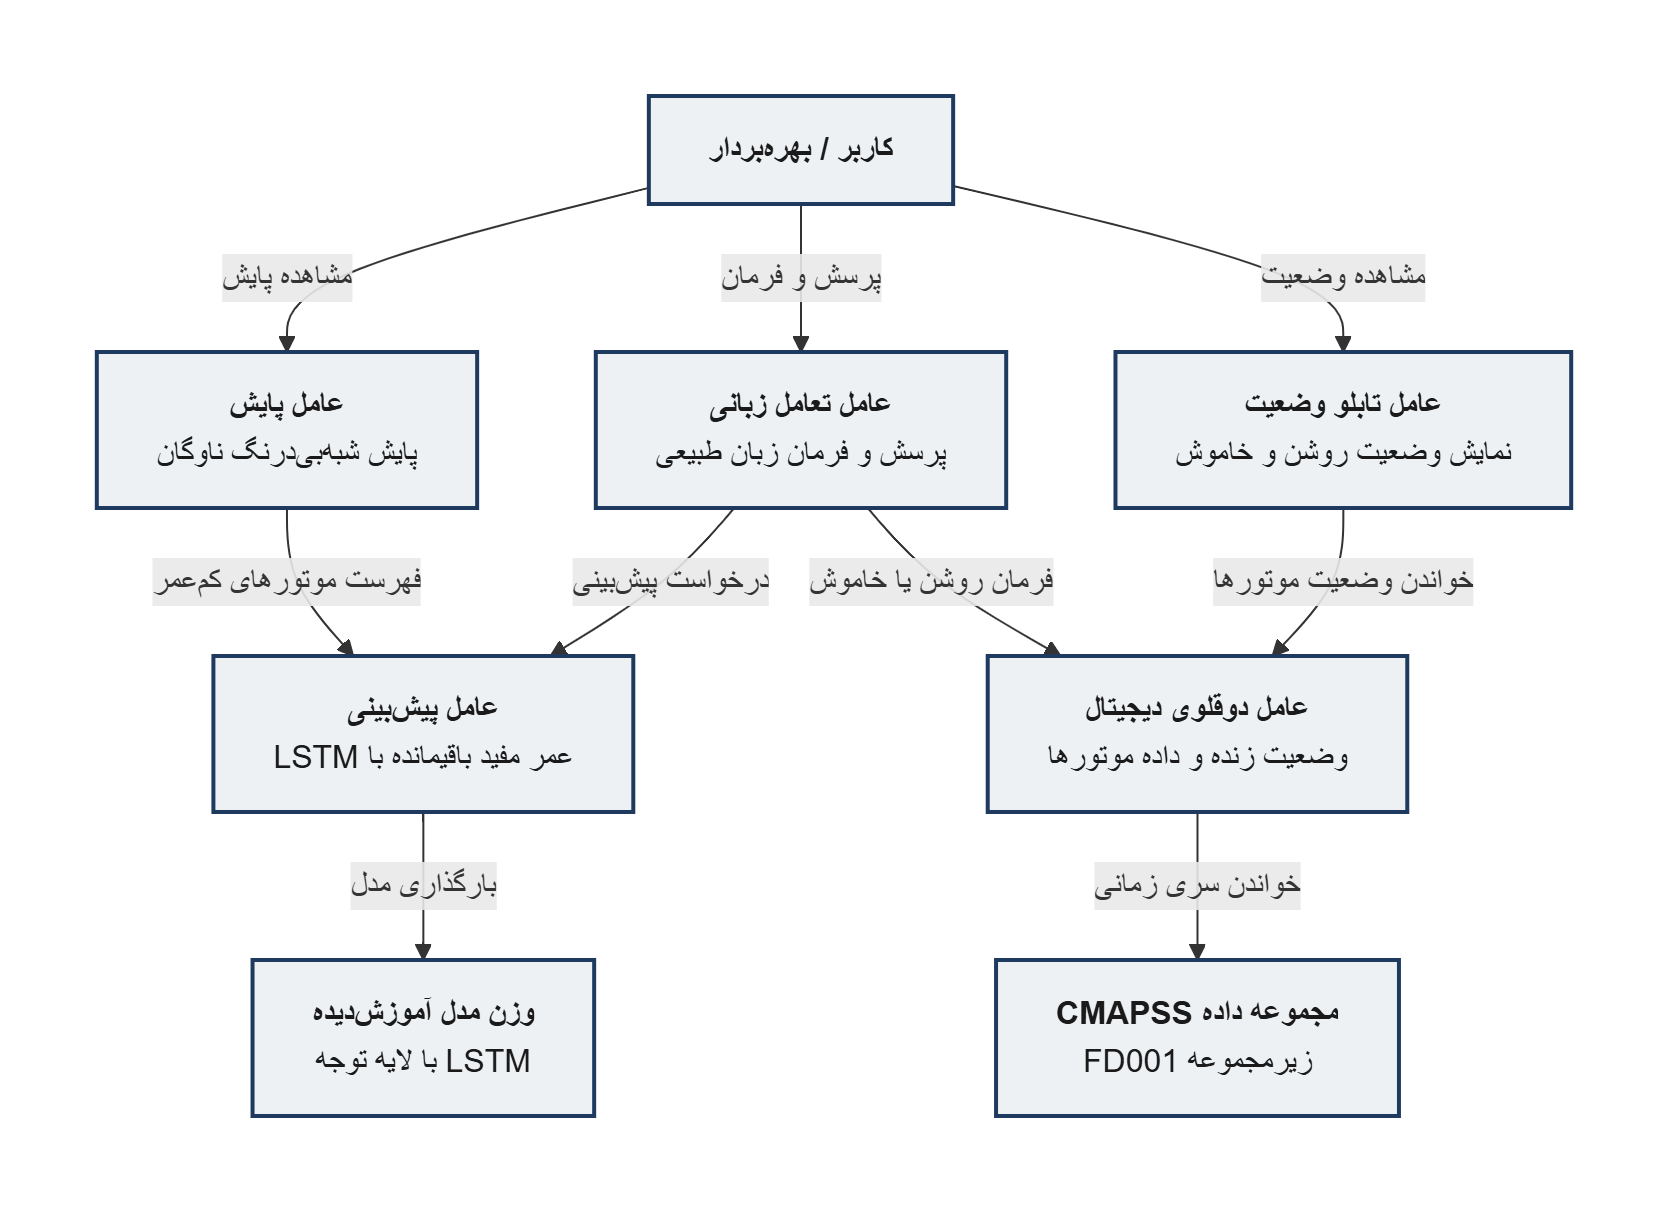
\includegraphics[width=0.95\textwidth]{images/impl_architecture.png}
	\caption{نمای کلی معماری پیاده‌سازی: پنج عامل سامانه، کاربر و جریان ارتباط میان آن‌ها}
	\label{fig:impl-component}
\end{figure}



\subsection{پشته فناوری}

پشته فناوری سامانه با توجه به دو ملاحظه اصلی انتخاب شده است. نخست، تناسب ابزار با وظیفه مورد نظر و دوم، سهولت یکپارچه‌سازی میان اجزای ناهمگون سامانه. برای آماده‌سازی داده و آموزش مدل از زبان \lr{Python} و کتابخانه‌های \lr{TensorFlow/Keras}، \lr{pandas} و \lr{scikit-learn} استفاده شده است. سرویس‌های \lr{API} با چارچوب \lr{FastAPI} پیاده‌سازی شده‌اند و رابط‌های کاربری با استفاده از \lr{React} توسعه یافته‌اند. عامل تعامل زبانی نیز بر بستر \lr{Dify Workflow} پیاده‌سازی شده است.

جدول \ref{tab:tech-stack} اجزای اصلی پشته فناوری را نشان می‌دهد.
\begin{table}[ht]
	\centering
	\caption{پشته فناوری سامانه به تفکیک مؤلفه}
	\label{tab:tech-stack}
	\begin{tabular}{p{4cm}p{9.5cm}}
		\toprule
		\textbf{مؤلفه} & \textbf{فناوری مورد استفاده} \\
		\midrule
		آموزش مدل &
		\lr{Python 3.10}، \lr{TensorFlow/Keras 2.17}،
		\lr{pandas}، \lr{scikit-learn 1.5.2}،
		\lr{Jupyter Notebook} \\
		
		\addlinespace
		عامل پیش‌بینی &
		\lr{FastAPI 0.115}، \lr{Uvicorn 0.32}،
		\lr{TensorFlow} \\
		
		\addlinespace
		عامل دوقلو &
		\lr{FastAPI}، \lr{pandas} \\
		
		\addlinespace
		عامل تعامل زبانی &
		\lr{Dify Workflow}،
		مدل‌های زبانی \lr{OpenAI} \\
		
		\addlinespace
		عامل پایش &
		\lr{React 18} + \lr{Create React App}،
		\lr{nginx} \\
		
		\addlinespace
		عامل \gls{Dashboard} &
		\lr{React 18} + \lr{Vite 4}،
		\lr{nginx} \\
		
		\addlinespace
		\gls{Orchestration} &
		\lr{Docker Compose} و \lr{Bash} \\
		
		\addlinespace
		داده &
		\gls{CMAPSS} \lr{FD001}
		(\lr{train/test/RUL}) \\
		\bottomrule
	\end{tabular}
\end{table}

\subsection{راه‌اندازی سرویس‌ها}

پنج سرویس اصلی سامانه در محیط آزمایشگاهی به‌صورت مستقل مستقر شده‌اند. از نظر وابستگی اجرایی، سرویس‌های هسته یعنی عامل دوقلو و عامل پیش‌بینی باید در دسترس باشند تا عامل‌های کاربردی بتوانند درخواست‌های اولیه خود را بدون خطای اتصال ارسال کنند. جدول \ref{tab:services-ports} مشخصات سرویس‌ها و درگاه‌‌های مورد استفاده را نشان می‌دهد.

\begin{table}[ht]
	\centering
	\caption{مشخصات سرویس‌های سامانه و پورت مورد استفاده}
	\label{tab:services-ports}
	\begin{tabular}{p{0.7cm}p{4cm}p{4cm}p{2.5cm}}
		\toprule
		\textbf{ردیف} & \textbf{سرویس} & \textbf{مسیر پیاده‌سازی} & \textbf{درگاه} \\
		\midrule
		۱ & عامل دوقلوی دیجیتال  & \lr{DTAgent/} & \lr{8001} \\
		۲ & عامل پیش‌بینی & \lr{lstm-rul-api/} & \lr{8000} \\
		۳ & عامل تعامل زبان طبیعی & \lr{dify/} & \lr{80/443} \\
		۴ & عامل \gls{Dashboard} & \lr{motor-dashboard/} & \lr{3000} \\
		۵ & عامل پایش & \lr{engine-monitor/} & \lr{3001} \\
		\bottomrule
	\end{tabular}
\end{table}

ارتباطات میان سرویس‌ها از طریق \lr{HTTP} انجام می‌شود و مسیرهای \lr{REST API} مرز عملیاتی میان عامل‌ها را مشخص می‌کنند. جدول \ref{tab:integration-matrix} مهم‌ترین ارتباط‌های میان سرویسی را نشان می‌دهد.

\begin{table}[ht]
	\centering
	\caption{ماتریس ارتباط میان سرویس‌های سامانه}
	\label{tab:integration-matrix}
	\begin{tabular}{p{3.5cm}p{3.5cm}p{2.2cm}p{4.2cm}}
		\toprule
		\textbf{مبدأ} & \textbf{مقصد} & \textbf{قرارداد} & \textbf{پارامتر یا پیکربندی} \\
		\midrule
		عامل تعامل زبان طبیعی  & عامل پیش‌بینی &
		\lr{HTTP GET} &
		\lr{lstm\_host\_addr} \\
		
		\addlinespace
		عامل تعامل زبان طبیعی  & عامل دوقلوی دیجیتال &
		\lr{HTTP POST} &
		\lr{dt\_host\_addr} \\
		
		\addlinespace
		عامل تعامل زبان طبیعی  & عامل پیش‌بینی &
		\lr{HTTP GET} &
		\lr{REACT\_APP\_API\_BASE\_URL} \\
		
		\addlinespace
		عامل \gls{Dashboard} & عامل دوقلوی دیجیتال &
		\lr{HTTP GET} &
		\lr{VITE\_API\_URL} \\
		
		%\addlinespace
		%\lr{docker-up.sh} & همه سرویس‌ها &
		%\lr{Compose} &
		%\lr{HOST\_IP} \\
		\bottomrule
	\end{tabular}
\end{table}

از منظر جریان داده، عامل زبان طبیعی تنها سرویسی است که در فرایندهای کنترلی، علاوه بر دریافت داده، امکان ارسال فرمان تغییر وضعیت به عامل دوقلوی دیجیتال را نیز دارد. بنابراین، این عامل در سطح کاربرد به‌عنوان واسط تصمیم‌گیری برای کاربر عمل می‌کند.



\section{روش استقرار سامانه}
\label{sec:deployment}

استقرار سامانه با استفاده از \lr{Docker} و مجموعه فایل‌های \lr{Docker Compose} انجام شده است. قطعه کد \lr{docker-up.sh} مسئول راه‌اندازی سرویس‌های اصلی است و به‌جای متکی بودن به یک فایل واحد، هر سرویس را در قالب پیکربندی مستقل خود اجرا می‌کند. این روش امکان مدیریت جداگانه چرخه عمر سرویس‌ها را فراهم می‌سازد و در محیط آزمایشگاهی برای تکرارپذیری اجرای آزمایش، مناسب است.

یکی از متغیرهای مهم محیطی، \lr{HOST\_IP} است. در محیط کانتینری، مقدار \lr{localhost} درون هر کانتینر به همان کانتینر اشاره می‌کند؛ ازاین‌رو برای دسترسی متقابل سرویس‌ها یا دسترسی مرورگر کاربر به رابط‌ها باید آدرس قابل دسترس میزبان به‌درستی تنظیم شود. در این پیاده‌سازی، همین آدرس برای برقراری ارتباط میان اجزای مختلف و دسترسی به رابط‌های کاربری استفاده شده است.

از نظر منابع سخت‌افزاری، آموزش مدل یادگیری عمیق پرهزینه‌ترین مرحله از نظر محاسباتی است و در محیط جداگانه با استفاده از \lr{GPU} انجام شده است. پس از پایان آموزش، وزن‌های مدل در سرویس پیش‌بینی قرار می‌گیرند و فرایند استنتاج در محیط اجرایی سامانه به \lr{GPU} مستقل نیاز ندارد. در نتیجه، در پیاده‌سازی حاضر میان محیط آموزش و محیط استقرار تفکیک ایجاد شده‌ است.


% -----------------------------------------------------------------------
\section{عامل دوقلوی دیجیتال}
\label{sec:impl-dtwin}

\subsection{نقش عامل در معماری}

عامل دوقلوی دیجیتال یکی از اجزای مرکزی سامانه است، زیرا هم مسئول ارائه داده‌های موتور به سایر اجزا است و هم وضعیت عملیاتی موتورها را نگهداری می‌کند. در پیاده‌سازی آزمایشگاهی، این سرویس بخشی از نقش لایه جمع‌آوری داده و بخشی از نقش لایه عامل‌های دوقلوی دیجیتال را بر عهده دارد. این تجمیع به دلیل ماهیت نمونه آزمایشگاهی صورت گرفته است و منطق مسئولیت‌ها در داخل سرویس تفکیک شده باقی مانده است.

برای هر موتور شناسه‌ای به‌صورت عدد صحیح در نظر گرفته شده است:

\[
k \in \{1,\ldots,100\}.
\]

و وضعیت عملیاتی هر موتور به‌صورت یک متغیر گسسته تعریف می‌شود:

\[
s_k\in\{\mathrm{ON},\mathrm{OFF}\}.
\]

در زمان راه‌اندازی، وضعیت تمام موتورهای موجود در مجموعه آزمون \lr{ON} در نظر گرفته می‌شود. سپس این وضعیت می‌تواند به‌صورت انتخابی برای تعدادی از موتورها یا به‌صورت سراسری برای کل موتور‌ها تغییر کند.

تصویر 
\ref{fig:impl-dtwin-arch}
سرویس‌های مربوط به عامل دوقلوی دیجیتال را به همراه ارتباط آن‌ها نشان می‌دهد. در این تصویر، شماره درگاه‌ دسترسی به هر سرویس و هم چنین قابل مشاهده است. 

\begin{figure}[H]
	\centering
	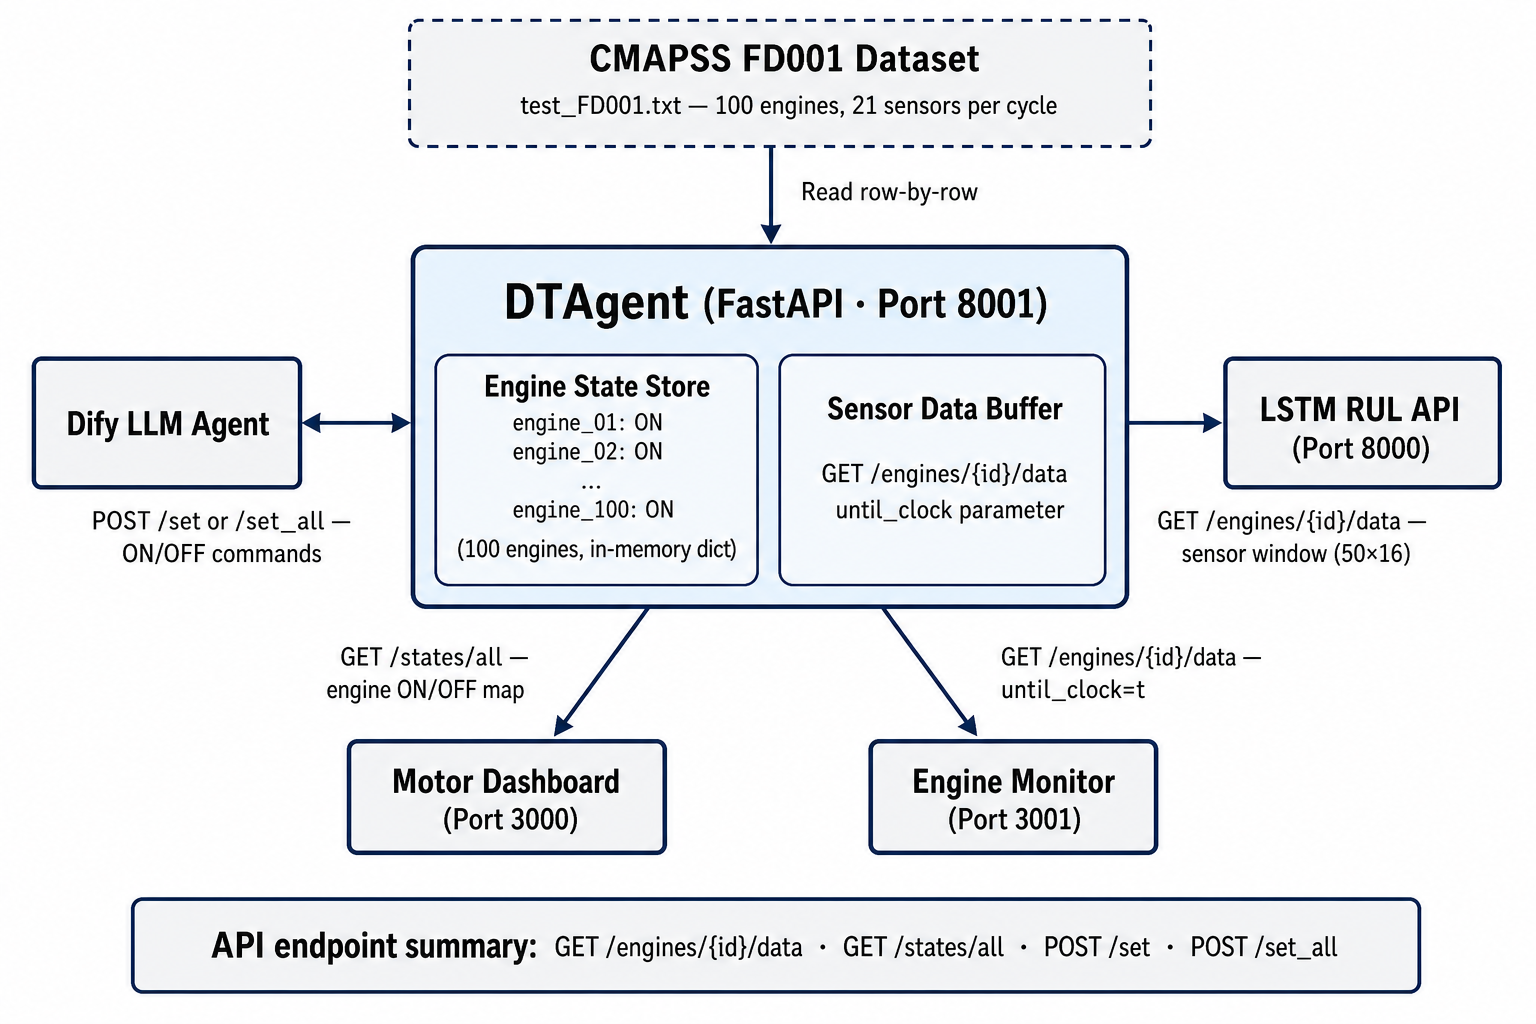
\includegraphics[width=0.90\textwidth]{images/agent_dtwin.png}
	\caption{ساختار داخلی عامل دوقلوی دیجیتال و ارتباط آن با داده‌های \lr{CMAPSS}، عامل زبانی و رابط تابلو وضعیت}
	\label{fig:impl-dtwin-arch}
\end{figure}


\subsection{ساختار داخلی سرویس}

عامل دوقلوی دیجیتال از سه جزء اصلی تشکیل شده است. جزء نخست مخزن وضعیت موتور است که در پیاده‌سازی فعلی به‌صورت یک ساختار درون‌ حافظه‌ نگهداری می‌شود. جزء دوم، حافظه موقت داده‌های حسگری است که از خواندن مکرر فایل داده جلوگیری می‌کند. جزء سوم، رابط \lr{REST API} است که دسترسی خواندنی به داده‌ها و دسترسی نوشتنی برای تغییر وضعیت را فراهم می‌کند. 


\subsection{رابط برنامه‌نویسی}

رابط برنامه‌نویسی عامل دوقلوی دیجیتال چند 
\gls{End Point}
برای دسترسی به داده و کنترل وضعیت فراهم می‌کند. نقاط پایانی خواندنی برای دریافت داده حسگرها و وضعیت موتور‌ها و نقاط پایانی نوشتنی برای تغییر وضعیت موتورها استفاده می‌شوند.

\begin{table}[ht]
	\centering
	\caption{نقاط پایانی رابط برنامه‌نویسی عامل دوقلو}
	\label{tab:dtwin-api}
	\begin{tabular}{p{1.2cm}p{5.2cm}p{3.2cm}p{3.2cm}}
		\toprule
		\textbf{متد} & \textbf{مسیر} & \textbf{ورودی} & \textbf{خروجی} \\
		\midrule
		\lr{GET} &
		\lr{/engines/\{engine\_number\}} &
		\lr{until\_clock} &
		داده‌‌های حسگرهای یک موتور \\
		
		\addlinespace
		\lr{GET} &
		\lr{/engines/states/all} &
		--- &
		وضعیت تمامی موتورها \\
		
		\addlinespace
		\lr{POST} &
		\lr{/engines/states/set?state=ON|OFF} &
		فهرست شناسه موتورها &
		وضعیت‌های به‌روزشده \\
		
		\addlinespace
		\lr{POST} &
		\lr{/engines/states/set\_all?state=ON|OFF} &
		وضعیت مقصد &
		وضعیت همه موتورها \\
		
		\addlinespace
		\lr{GET} &
		\lr{/} &
		--- &
		پیام سلامت سرویس \\
		\bottomrule
	\end{tabular}
\end{table}

پارامتر \lr{until\_clock} یکی از عناصر اصلی سازوکار شبیه‌سازی زمانی است. عامل مصرف‌کننده می‌تواند به‌جای دریافت کل تاریخچه موتور، تنها داده‌های موجود تا چرخه مشخصی را درخواست کند. از این طریق، فایل ایستا به یک منبع داده پویا تبدیل می‌شود که امکان اجرای آزمایش‌های شبه‌بی‌درنگ را فراهم می‌کند.


\subsection{محدودیت وضعیت درون‌حافظه‌ای}

وضعیت \lr{ON/OFF} در حافظه سرویس نگهداری می‌شود. در نتیجه، با راه‌اندازی مجدد کانتینر، وضعیت اولیه مجدداً ایجاد می‌شود و موتورها به حالت \lr{ON} بازمی‌گردند. همچنین به دلیل هزینه بالای حافظه موقت، در صورت بالا رفتن حجم داده‌ای که ذخیره می‌شود، مقیاس‌پذیری و افزایش ظرفیت آن دشوار است. زمانی این امکان وجود دارد که تعداد موتور‌ها بسیار بالا و وضعیت ذخیره شده برای هرکدام بسیار پر حجم -- شامل مؤلفه‌های زیاد و دارای اطلاعات باینری مانند تصویر یا فیلم -- باشد. با این حال، تا زمانی که این روش ذخیره‌سازی مشکل هزینه و بازدهی ایجاد نکند، می‌توان به استفاده آن ادامه داد.


% -----------------------------------------------------------------------
\section{عامل پیش‌بینی عمر مفید باقیمانده}
\label{sec:impl-lstm}

\subsection{معماری شبکه پیش‌بینی}
پس از آمادگی اولیه داده که در فصل
\ref{chap:methodology}
توضیح داده شد، به معماری شبکه پبش‌بینی پرداخته می‌شود.
مدل پیش‌بینی از یک شبکه بازگشتی دو لایه تشکیل شده است. لایه نخست دارای ۱۰۰ واحد و لایه دوم دارای ۵۰ واحد است. پس از هر لایه بازگشتی، یک لایه \lr{Dropout} با نرخ ۰٫۲ برای کنترل بیش‌برازش قرار گرفته است. در انتهای شبکه نیز یک لایه \lr{Dense} تک‌واحدی با فعال‌سازی خطی قرار دارد که مقدار عددی \gls{RUL} را تولید می‌کند.

ساختار کلی مدل در جدول \ref{tab:lstm-arch} خلاصه شده است.

\begin{table}[ht]
	\centering
	\caption{معماری شبکه پیش‌بینی عمر مفید باقیمانده}
	\label{tab:lstm-arch}
	\begin{tabular}{p{4cm}p{4cm}p{5cm}}
		\toprule
		\textbf{لایه} & \textbf{مشخصات} & \textbf{نقش} \\
		\midrule
		\lr{Input} &
		$50\times14$ &
		دریافت توالی ۵۰ چرخه‌ای \\
		
		\addlinespace
		\lr{LSTM-1} &
		۱۰۰ واحد &
		استخراج الگوهای زمانی \\
		
		\addlinespace
		\lr{Dropout-1} &
		نرخ ۰٫۲ &
		کاهش خطر بیش‌برازش \\
		
		\addlinespace
		\lr{LSTM-2} &
		۵۰ واحد &
		استخراج نمایش زمانی سطح بالاتر \\
		
		\addlinespace
		\lr{Dropout-2} &
		نرخ ۰٫۲ &
		منظم‌سازی مدل \\
		
		\addlinespace
		\lr{Dense} &
		یک واحد، خطی &
		تولید مقدار عددی \gls{RUL} \\
		\bottomrule
	\end{tabular}
\end{table}



\subsection{پارامترهای آموزش}

پارامترهای اصلی آموزش در جدول \ref{tab:lstm-hyperparams} ارائه شده‌اند.

\begin{table}[ht]
	\centering
	\caption{پارامترهای اصلی آموزش مدل پیش‌بینی}
	\label{tab:lstm-hyperparams}
	\begin{tabular}{p{5cm}p{8cm}}
		\toprule
		\textbf{پارامتر} & \textbf{مقدار} \\
		\midrule
		بهینه‌ساز &
		\lr{RMSprop} \\
		
		\addlinespace
		اندازه دسته &
		۲۰۰ \\
		
		\addlinespace
		تعداد دوره‌های آموزش &
		۶۰ \\
		
		\addlinespace
		نسبت اعتبارسنجی &
		۰٫۰۵ \\
		
		\addlinespace
		تابع زیان &
		\lr{PinballLoss}، $\tau=0.125$ \\
		
		\addlinespace
		معیارهای پایش &
		\lr{MAE} و $R^2$ \\
		
		\bottomrule
	\end{tabular}
\end{table}

در پیاده‌سازی، مقادیر جدول \ref{tab:lstm-hyperparams} مستقیماً در فرایند آموزش شبکه اعمال شده‌اند. بهینه‌ساز \lr{RMSprop} برای به‌روزرسانی تطبیقی وزن‌ها در شبکه بازگشتی به‌کار رفته است. اندازه دسته برابر ۲۰۰ تعیین شده تا در هر گام آموزشی، ۲۰۰ توالی ۵۰ چرخه‌ای به‌صورت یکجا پردازش شود؛ این مقدار میان هزینه حافظه و پایداری تعادل برقرار می‌کند. آموزش در ۶۰ دوره کامل انجام شده و در هر دوره وزن‌ها روی کل مجموعه آموزش بازبینی می‌شوند. نسبت اعتبارسنجی، ۰٫۰۵ از توالی‌های آموزشی را بدون مشارکت در به‌روزرسانی وزن‌ها کنار می‌گذارد تا روند تعمیم‌پذیری در طول آموزش قابل پایش باشد؛ این بخش جدا از مجموعه آزمون است که پیش‌تر برای ارزیابی نهایی نگه داشته شده است. تابع زیان اصلی \lr{PinballLoss} با $\tau=0.125$ استفاده شده است که به صورت مفصل در بخش
\ref{sec:cmapss-prediction-agent}
توضیح داده می‌شود.
. معیارهای \lr{MAE} و $R^2$ نیز علاوه بر تابع زیان در هر دوره ثبت شده‌اند تا علاوه بر مقدار هدف بهینه‌سازی، خطای مطلق و میزان توضیح‌پذیری مدل قابل پیگیری باشد.


\subsection{سرویس پیش‌بینی}

پس از پایان آموزش، مدل در قالب یک سرویس مستقل \lr{REST API} مبتنی بر \lr{FastAPI} مورد استفاده قرار گرفته است. مدل در هنگام راه‌اندازی سرویس بارگذاری می‌شود تا هزینه بارگذاری اولیه در اولین درخواست کاهش یابد. ساختار بارگذاری مدل به‌گونه‌ای است که در صورت بروز خطا، سرویس دچار شکست نشود و نقاط پایانی بتوانند خطای مناسب را گزارش کنند.

مهم‌ترین نقاط پایانی سرویس در جدول \ref{tab:lstm-api} ارائه شده‌اند.

\begin{table}[ht]
	\centering
	\caption{نقاط پایانی عامل پیش‌بینی}
	\label{tab:lstm-api}
	\begin{tabular}{p{1.2cm}p{7.5cm}p{5cm}}
		\toprule
		\textbf{متد} & \textbf{مسیر} & \textbf{کاربرد} \\
		\midrule
		\lr{GET} &
		\lr{/api/health} &
		بررسی سلامت سرویس \\
		
		\addlinespace
		\lr{GET} &
		\lr{/api/predict/predict\_rul/\{engine\_number\}} &
		پیش‌بینی RUL برای موتور مشخص \\
		
		\addlinespace
		\lr{GET} &
		\lr{/api/predict/engines\_with\_low\_rul/} &
		شناسایی موتورهای کم‌عمر \\
		
		\addlinespace
		\lr{POST} &
		\lr{/api/predict/predict\_new\_engine\_rul/} &
		پیش‌بینی برای توالی دلخواه \\
		\bottomrule
	\end{tabular}
\end{table}

نقطه پایانی \lr{predict\_rul} پرکاربردترین مسیر سرویس است. این نقطه پس از دریافت شناسه موتور، داده لازم را از مجموعه آزمون استخراج می‌کند، آخرین پنجره زمانی معتبر را می‌سازد، مدل را اجرا می‌کند و مقدار \gls{RUL} را در قالب پاسخ \lr{JSON} بازمی‌گرداند.

یک نمونه ساختار پاسخ به‌صورت زیر است:

\begin{latin}
	\begin{verbatim}
		{
			"engine_number": 10,
			"predicted_rul": 164.67
		}
	\end{verbatim}
\end{latin}

این ساختار باعث می‌شود خروجی مدل عددی از منطق واسط کاربر مستقل باقی بماند و سایر عامل‌ها بتوانند بدون وابستگی به قالب نمایشی، مقدار پیش‌بینی‌شده را مصرف کنند.


% -----------------------------------------------------------------------
\section{عامل تعامل زبانی}
\label{sec:impl-llm}

\subsection{الگوی طراحی}

عامل تعامل زبانی واسط میان کاربر و خدمات تخصصی سامانه است. به‌جای آنکه مدل زبانی آزادانه مسیر انجام هر درخواست را تعیین کند، یک \gls{Workflow} از پیش تعریف‌شده در \lr{Dify} ایجاد شده است. در این ساختار، ابتدا سوال کاربر دسته‌بندی می‌شود و سپس درخواست مطابق همان دسته، به یک مسیر مشخص هدایت می‌گردد.

انتخاب \gls{Workflow} کنترل‌شده برای مسئله حاضر از آن جهت اهمیت دارد که بدون نیاز به نوشتن کد سطح پایین، می‌توان قابلیت‌های متنوعی به عامل زبان طبیعی اضافه کرد و دستورات جدیدی پشتیبانی داد. بنابراین، استفاده از \gls{Workflow} برای ایجاد عامل،‌ انعطاف‌پذیری قابل توجهی را برای عامل ایجاد می‌کند به طوری که در هر لحظه،‌ بتوان به سادگی کارکرد آن را تغییر داد یا بهبود بخشید. این دیدگاه با پژوهش‌های جدید درباره ادغام مدل‌های زبانی بزرگ و دوقلوهای دیجیتال که بر نقش مدل زبانی به‌عنوان واسط تعامل و تحلیل سطح‌بالا تأکید می‌کنند، هم‌راستا است \cite{CHEN2025102982LLMDT}.

تصویر
\ref{fig:impl-llm-arch}
معماری داخلی عامل مدل زبانی بزرگ را که با استفاده از \lr{Dify} ایجاد شده است، نشان می‌دهد. در ابتدا طبق سوالی که کاربر پرسیده است، تشخیص داده می‌شود که سوال کاربر در کدام دسته قرار میگیرد. سپس بر اساس دسته‌ای که تشخیص داده شده است، نقاط پایانی مناسب استفاده می‌شود. در نهایت هم پاسخ مناسب برای کاربر ایجاد شده و نمایش داده می‌شود.
تصویر 
\ref{fig:dify-workflow-screenshot}
نیز \gls{Workflow} ایجاد شده در محیط \lr{Dify} نشان داده می‌شود.

\begin{figure}[H]
	\centering
	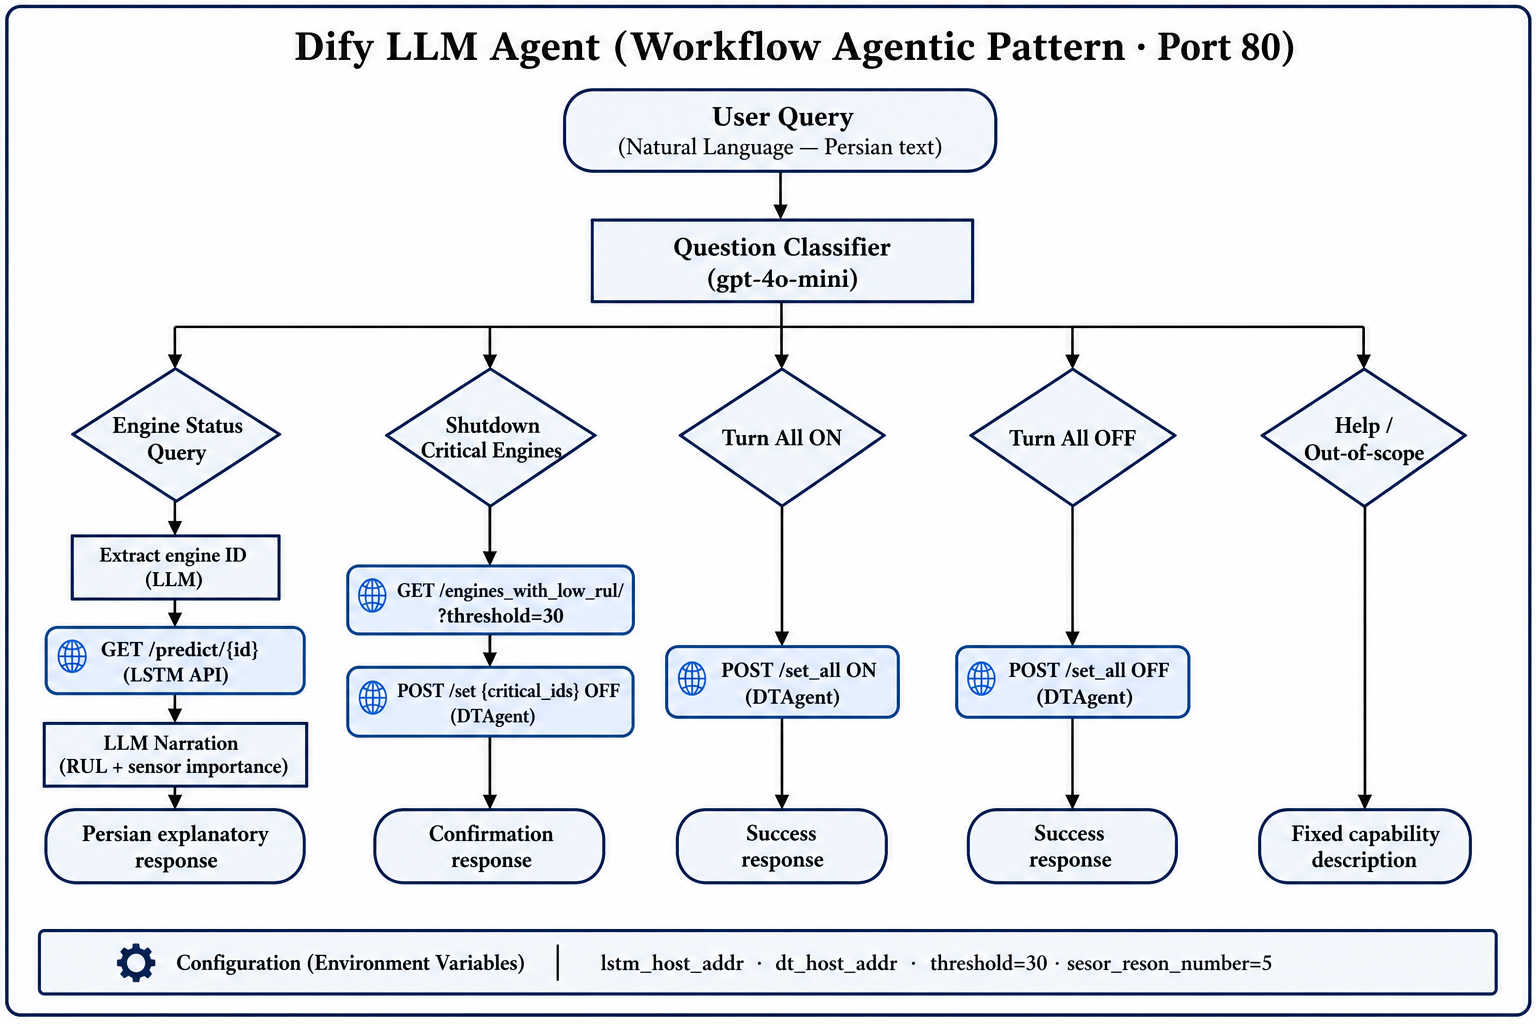
\includegraphics[width=0.90\textwidth]{images/agent_dify_llm.png}
	\caption{ساختار Workflow عامل تعامل زبانی و مسیرهای اصلی پردازش درخواست}
	\label{fig:impl-llm-arch}
\end{figure}

\begin{figure}[H]
	\centering
	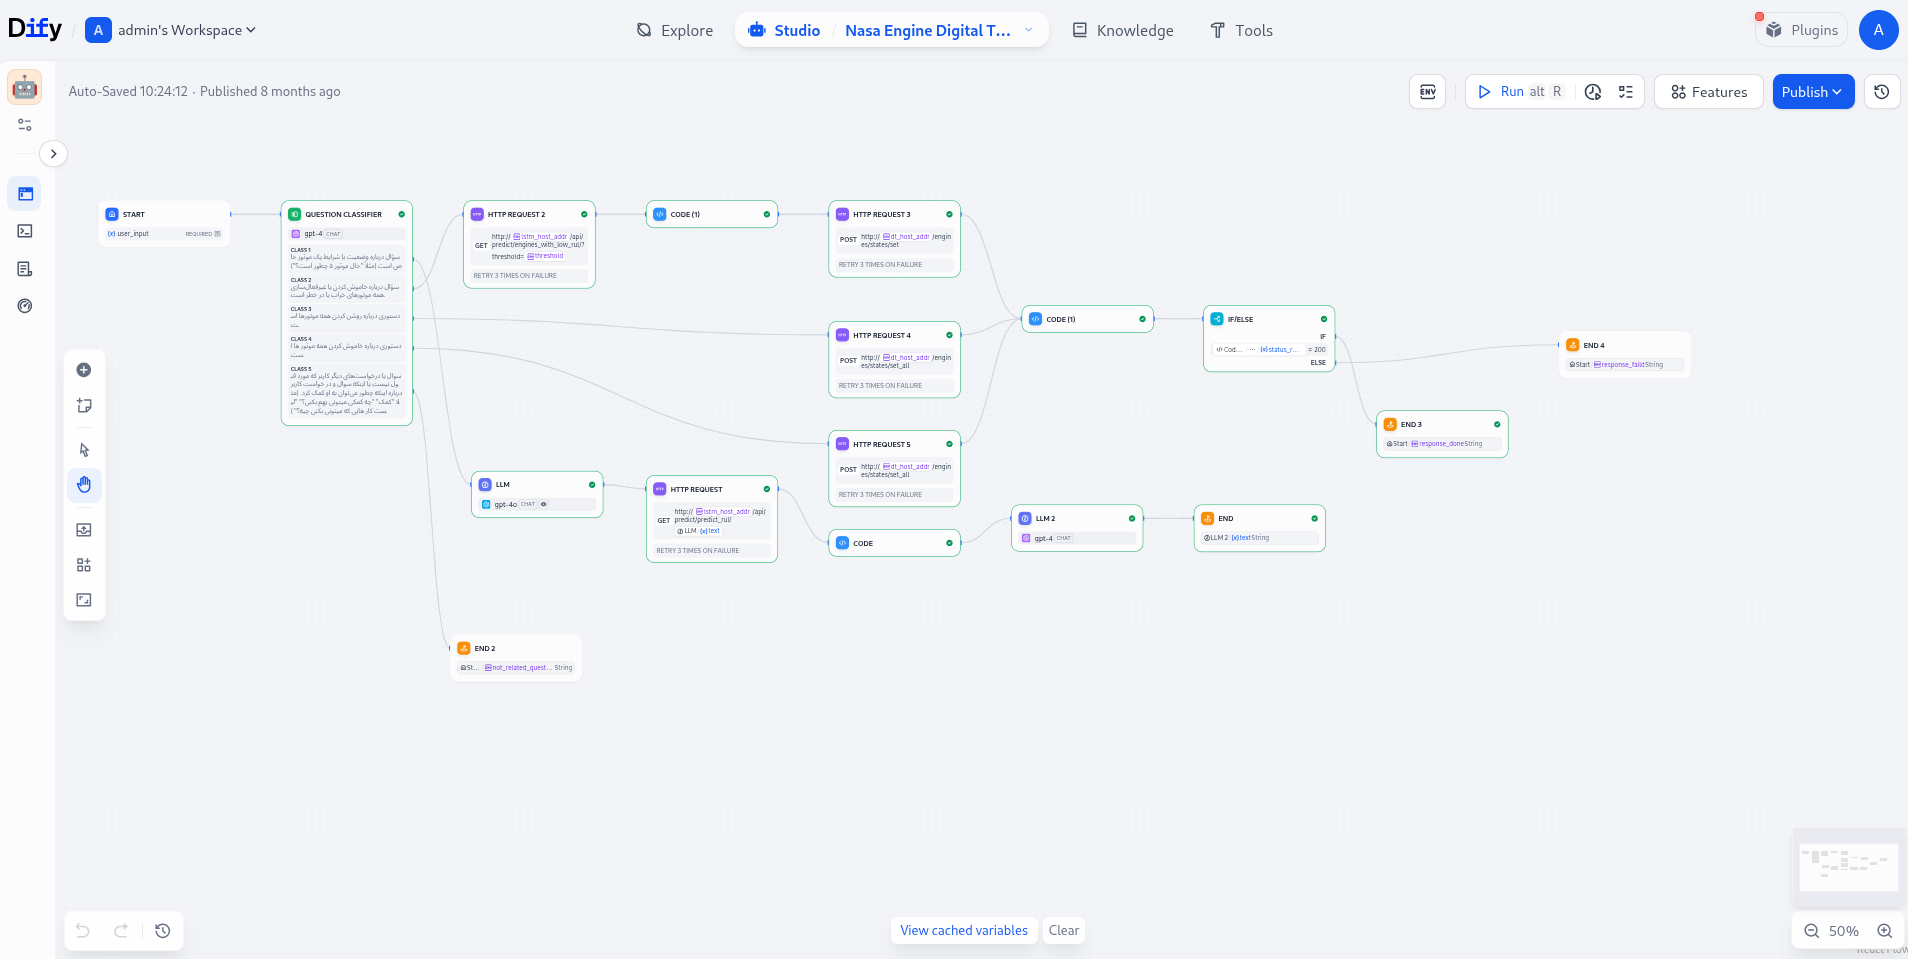
\includegraphics[width=0.92\textwidth]{images/dify_workflow_screenshot_2.png}
	\caption{نمای Workflow پیاده‌سازی‌شده در محیط Dify و انشعاب مسیرهای تصمیم بر اساس سوال کاربر}
	\label{fig:dify-workflow-screenshot}
\end{figure}

\subsection{فضای نیت و مسیرهای تصمیم}

فضای نیت بر اساس قابلیت‌های مورد نیاز سامانه تعریف شده است. در مجموع پنج کلاس اصلی برای درخواست کاربر، در نظر گرفته شده است که هر کدام مسیر اجرایی مشخصی دارند.

\begin{table}[ht]
	\centering
	\caption{کلاس‌های نیت و اقدام متناظر در عامل تعامل زبانی}
	\label{tab:intent-space}
	\begin{tabular}{p{0.7cm}p{3.6cm}p{4cm}p{5cm}}
		\toprule
		\textbf{ردیف} & \textbf{نیت} & \textbf{نمونه ورودی} & \textbf{اقدام} \\
		\midrule
		۱ &
		وضعیت یک موتور &
		«موتور ۱ چه زمانی خراب می‌شود؟» &
		استخراج شناسه و فراخوانی سرویس پیش‌بینی \\
		
		\addlinespace
		۲ &
		خاموش‌سازی موتورهای در خطر &
		«موتورهای در خطر را خاموش کن» &
		دریافت فهرست کم‌عمرها و ارسال فرمان \lr{OFF} \\
		
		\addlinespace
		۳ &
		روشن کردن همه موتورها &
		«همه موتورها را روشن کن» &
		ارسال فرمان \lr{set\_all ON} \\
		
		\addlinespace
		۴ &
		خاموش کردن همه موتورها &
		«همه موتورها را خاموش کن» &
		ارسال فرمان \lr{set\_all OFF} \\
		
		\addlinespace
		۵ &
		راهنما یا خارج از حوزه &
		«چه کمکی می‌توانی بکنی؟» &
		نمایش فهرست قابلیت‌های سامانه \\
		\bottomrule
	\end{tabular}
\end{table}

یکی از ویژگی‌های این طراحی آن است که همه شاخه‌ها نیازمند فراخوانی مدل زبانی بزرگ نیستند. در شاخه‌های فرمان سراسری، درخواست پس از تشخیص نیت می‌تواند مستقیماً به فراخوانی مناسب \lr{HTTP} تبدیل شود. در مقابل، شاخه وضعیت موتور به پردازش زبانی بیشتری نیاز دارد، زیرا ابتدا باید شناسه موتور از متن طبیعی استخراج و سپس پاسخ قابل فهم برای کاربر تولید شود.

\subsection{نقاط پایانی HTTP و پیکربندی}

نقاط پایانی \lr{HTTP} پل ارتباطی میان \gls{Workflow} و سرویس‌های تخصصی هستند. مسیرهای اصلی این نقاط در جدول \ref{tab:http-nodes} ارائه شده‌اند.

\begin{table}[ht]
	\centering
	\caption{نقاط پایانی HTTP مورد استفاده در Workflow عامل زبانی}
	\label{tab:http-nodes}
	\begin{tabular}{p{1.5cm}p{7cm}p{5.5cm}}
		\toprule
		\textbf{متد} & \textbf{مسیر} & \textbf{کاربرد} \\
		\midrule
		\lr{GET} &
		\lr{/api/predict/predict\_rul/\{id\}} &
		دریافت RUL موتور مشخص \\
		
		\addlinespace
		\lr{GET} &
		\lr{/api/predict/engines\_with\_low\_rul/?threshold=} &
		دریافت فهرست موتورهای کم‌عمر \\
		
		\addlinespace
		\lr{POST} &
		\lr{/engines/states/set?state=OFF} &
		خاموش‌سازی انتخابی \\
		
		\addlinespace
		\lr{POST} &
		\lr{/engines/states/set\_all?state=ON} &
		روشن کردن سراسری \\
		
		\addlinespace
		\lr{POST} &
		\lr{/engines/states/set\_all?state=OFF} &
		خاموش کردن سراسری \\
		\bottomrule
	\end{tabular}
\end{table}

متغیرهای محیطی به‌عنوان لایه پیکربندی میان \gls{Workflow} و زیرساخت سرویس‌ها عمل می‌کنند. مهم‌ترین متغیرها در جدول \ref{tab:env-vars} آمده‌اند.

\begin{table}[ht]
	\centering
	\caption{متغیرهای محیطی اصلی عامل تعامل زبانی}
	\label{tab:env-vars}
	\begin{tabular}{p{4.5cm}p{3.5cm}p{5cm}}
		\toprule
		\textbf{متغیر} & \textbf{نمونه مقدار} & \textbf{کاربرد} \\
		\midrule
		\lr{lstm\_host\_addr} &
		\lr{10.226.63.45:8000} &
		آدرس عامل پیش‌بینی \\
		
		\addlinespace
		\lr{dt\_host\_addr} &
		\lr{10.226.63.45:8001} &
		آدرس عامل دوقلو \\
		
		\addlinespace
		\lr{threshold} &
		\lr{30} &
		آستانه تشخیص موتور در خطر \\
		
		\addlinespace
		\lr{sesor\_reson\_number} &
		\lr{5} &
		تعداد متغیرهای نمایش‌داده‌شده در پاسخ \\
		
		\addlinespace
		\lr{response\_done} &
		متن فارسی &
		پیام موفقیت عملیات \\
		
		\addlinespace
		\lr{not\_related\_question} &
		متن فارسی &
		پاسخ خارج از حوزه \\
		\bottomrule
	\end{tabular}
\end{table}


\subsection{نمونه‌های عملیاتی}

در نخستین نمونه
\ref{qa:llm-help}
، کاربر پرسشی خارج از محدوده عملیاتی سامانه مطرح می‌کند یا از عامل می‌خواهد که قابلیت‌های خود را بیان کند. عامل با فعال کردن شاخه راهنما، قابلیت‌های قابل ارائه را بدون اجرای عملیات تحلیلی اضافی نمایش می‌دهد.

%\begin{figure}[H]
%	\centering
%	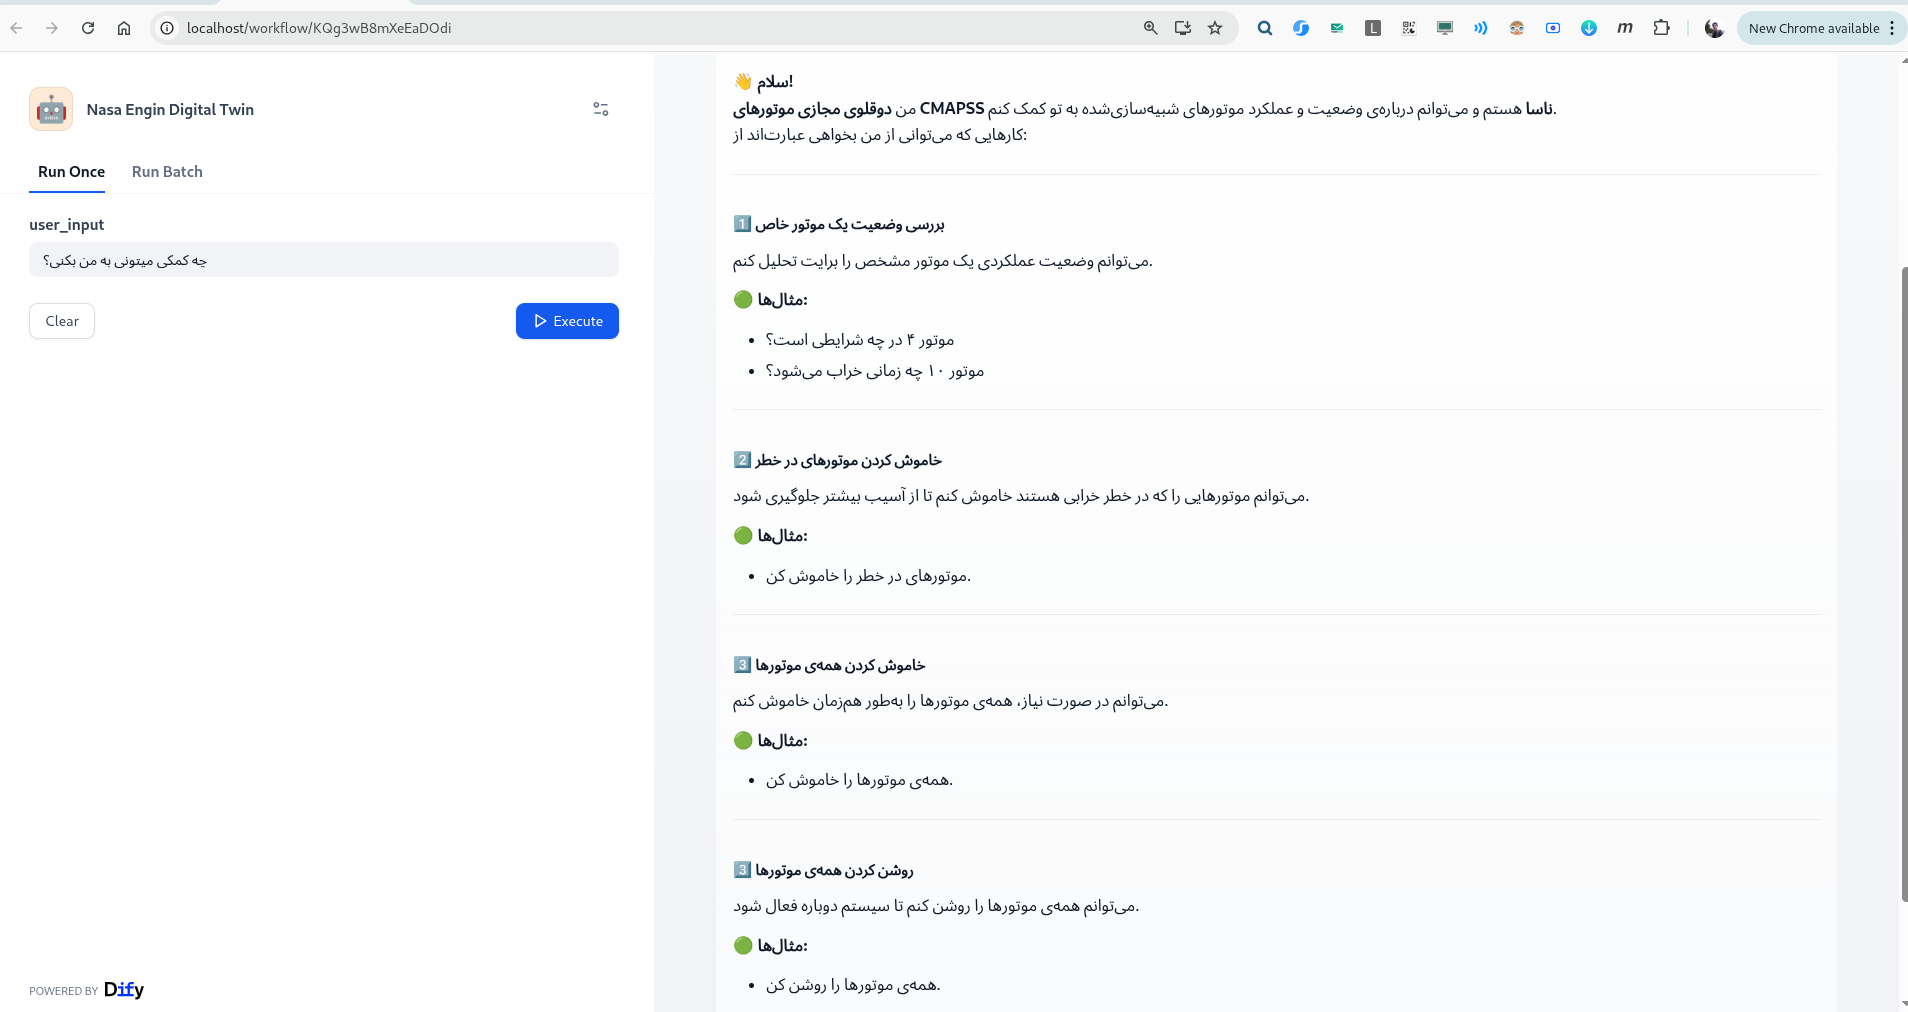
\includegraphics[width=1\textwidth]{images/llm_help_response.png}
%	\caption{نمونه پاسخ عامل زبانی در شاخه راهنما و معرفی قابلیت‌های سامانه}
%	\label{fig:llm-help}
%\end{figure}



% ══ گفتگو ════════════════════════════════════════════════════
\begin{figure}[h]
	\centering
	\begin{minipage}{0.92\textwidth}
		
		%% ── پرسش کاربر ───────────────────────────────────────────
		\begin{userBox}
			\textbf{کاربر:}\ چه کمکی می‌توانی به من بکنی؟
		\end{userBox}
		
		%% ── پاسخ دستیار ──────────────────────────────────────────
		\begin{botBox}
			\textbf{دستیار (ناسا):}
			
			سلام! من \textbf{ناسا} هستم و می‌توانم دربارهٔ وضعیت و عملکرد موتورهای
			شبیه‌سازی‌شدهٔ دوقلوی مجازی موتورهای \textbf{CMAPSS} به تو کمک کنم.
			کارهایی که می‌توانی از من بخواهی عبارت‌اند از:
			
			\medskip
			
			\qaSection{۱}{بررسی وضعیت یک موتور خاص}
			
			می‌توانم وضعیت عملکردی یک موتور مشخص را برایت تحلیل کنم.
			
			\exLabel
			\begin{itemize}[rightmargin=1.5em, topsep=2pt, itemsep=1pt]
				\item موتور ۴ در چه شرایطی است؟
				\item موتور ۱۰ چه زمانی خراب می‌شود؟
			\end{itemize}
			
			\medskip
			\qaSection{۲}{خاموش کردن موتورهای در خطر}
			
			می‌توانم موتورهایی را که در خطر خرابی هستند خاموش کنم تا از آسیب بیشتر جلوگیری شود.
			
			\exLabel
			\begin{itemize}[rightmargin=1.5em, topsep=2pt, itemsep=1pt]
				\item موتورهای در خطر را خاموش کن.
			\end{itemize}
			
			\medskip
			\qaSection{۳}{خاموش کردن همهٔ موتورها}
			
			می‌توانم در صورت نیاز، همهٔ موتورها را به‌طور هم‌زمان خاموش کنم.
			
			\exLabel
			\begin{itemize}[rightmargin=1.5em, topsep=2pt, itemsep=1pt]
				\item همهٔ موتورها را خاموش کن.
			\end{itemize}
			
			\medskip
			\qaSection{۴}{روشن کردن همهٔ موتورها}
			
			می‌توانم همهٔ موتورها را روشن کنم تا دوباره سیستم فعال شود.
			
			\exLabel
			\begin{itemize}[rightmargin=1.5em, topsep=2pt, itemsep=1pt]
				\item همهٔ موتورها را روشن کن.
			\end{itemize}
			
		\end{botBox}
		
	\end{minipage}
	\caption{نمونه پاسخ عامل زبانی در شاخه راهنما و معرفی قابلیت‌های سامانه}
	\label{qa:llm-help}
\end{figure}


در نمونه دوم که در تصویر 
\ref{qa:llm-engine-query-2}
قابل مشاهده است، پرس‌وجو برای موتور ۲ را نمایش می‌دهد. موتور ۲ دارای مقدار پیش‌بینی‌شده عمر مفید باقیمانده برابر ۶۳.۷۷ چرخه است. این مقدار نسبت به آستانه که ۳۰ چرخه است فاصله زیادی دارد و در نتیجه موتور در محدوده عادی قرار می‌گیرد. 
همچنین در نمونه سوم که در تصویر
\ref{qa:llm-engine-query-24}
مشاهده می‌شود، پرس‌وجو برای موتور ۲۴ را نمایش می‌دهد. موتور ۲۴ دارای مقدار عمر مفید باقیمانده برابر ۲۷.۴۱ چرخه است که پایین‌تر از آستانه ۳۰ قرار می‌گیرد و در نتیجه وضعیت بحرانی برای آن گزارش می‌شود.
\


% \begin{figure}[H]
% 	\centering
% 	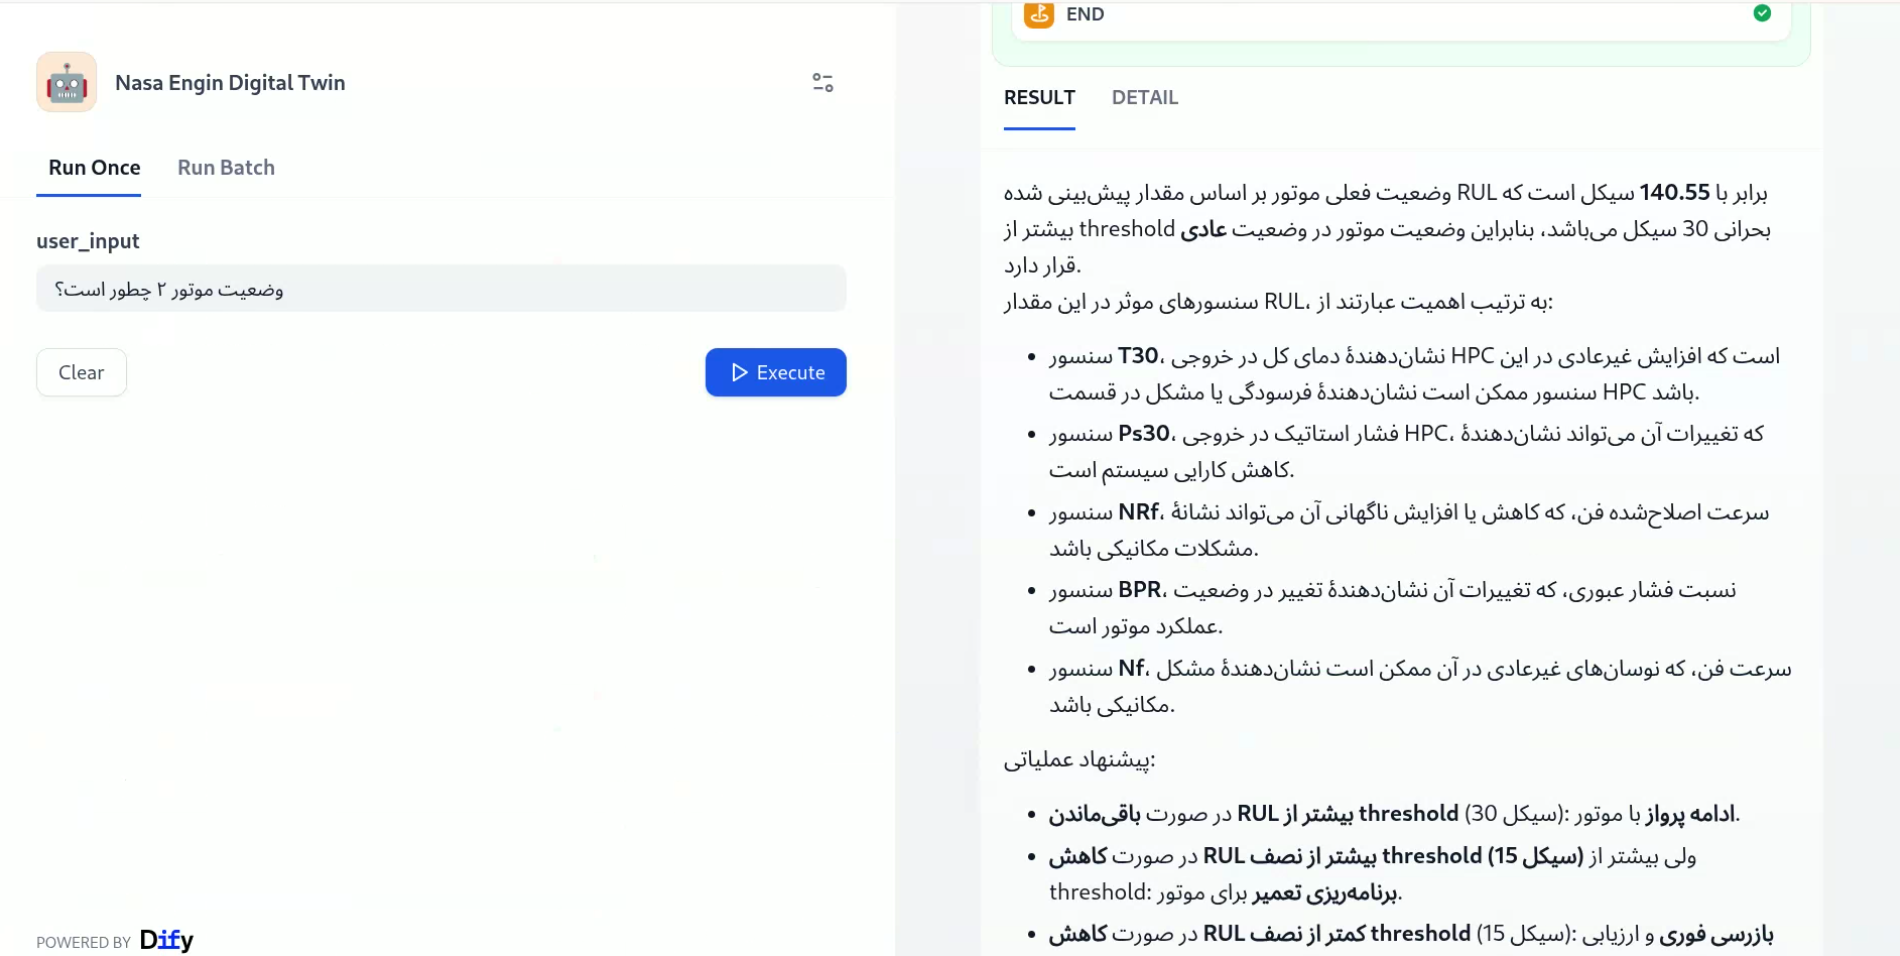
\includegraphics[width=0.85\textwidth]{images/llm_engine2_query.png}
% 	\caption{نمونه پاسخ عامل زبانی برای پرس‌وجوی وضعیت موتور و تبدیل خروجی عددی به روایت فارسی ساختاریافته}
% 	\label{fig:llm-engine-query-2}
% \end{figure}


% \begin{figure}[H]
% 	\centering
% 	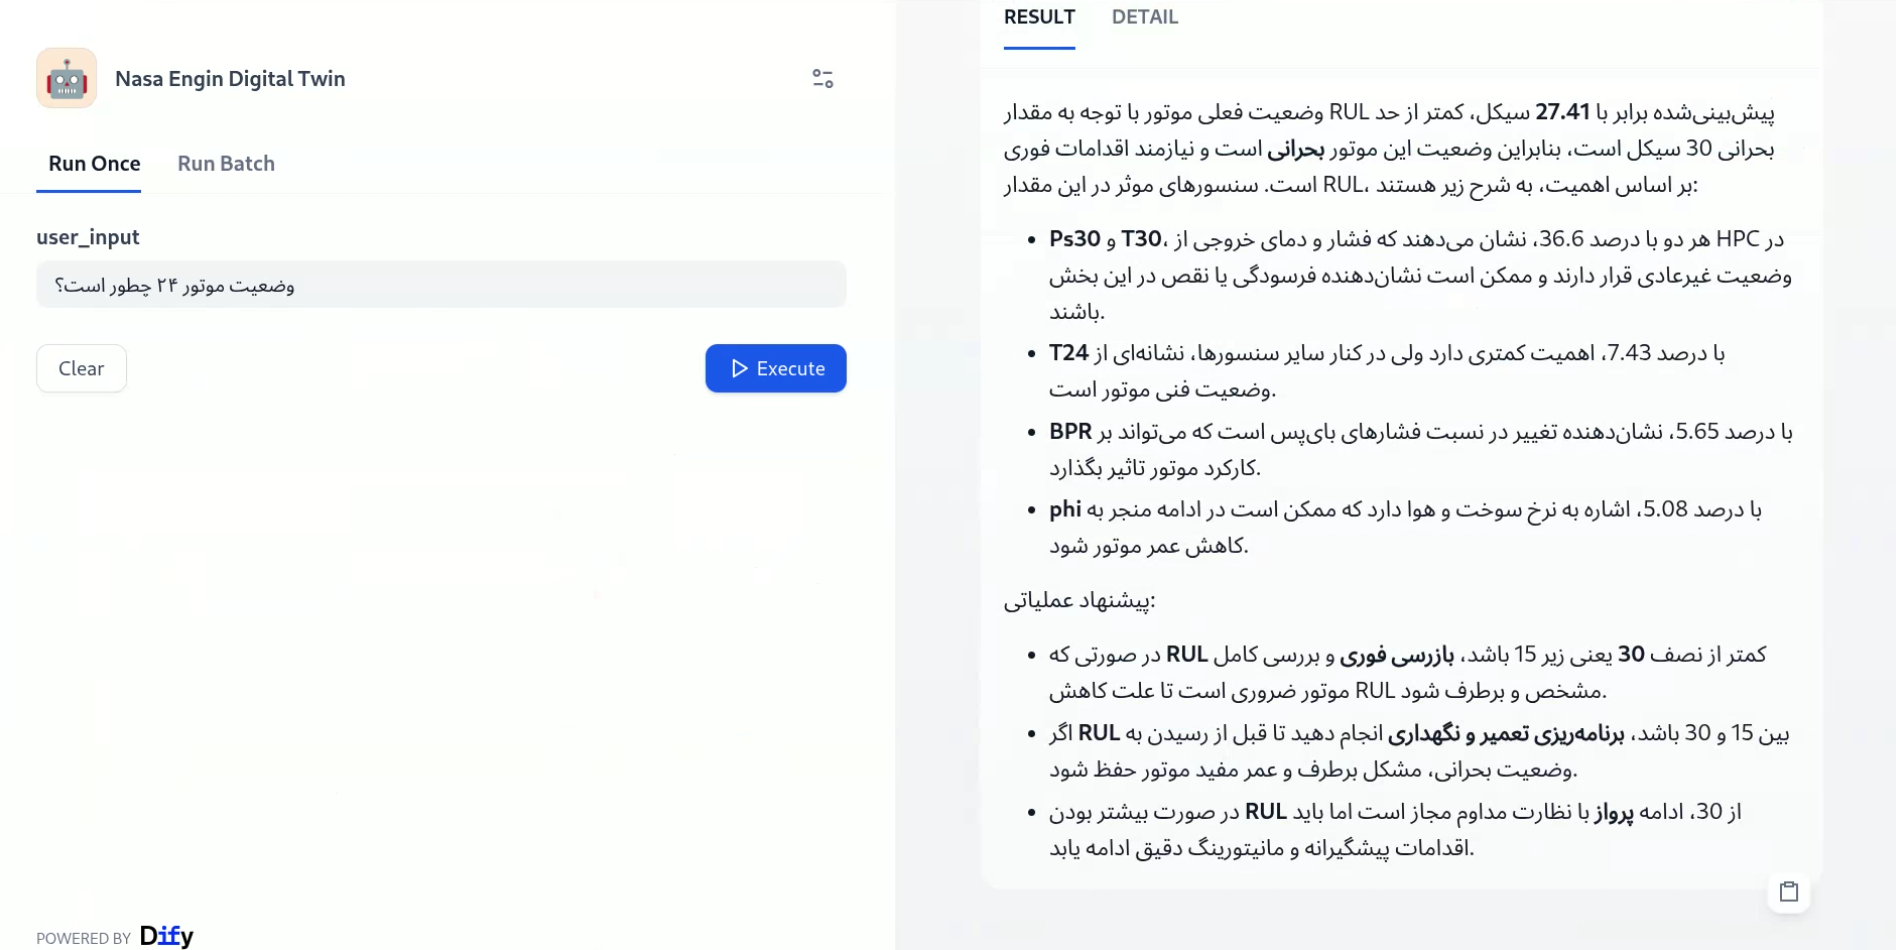
\includegraphics[width=0.85\textwidth]{images/llm_engine24_query.png}
% 	\caption{نمونه پاسخ عامل زبانی برای پرس‌وجوی وضعیت موتور  ۲۴ و تبدیل خروجی عددی به روایت فارسی ساختاریافته}
% 	\label{fig:llm-engine-query-24}
% \end{figure}

% ════════════════════════════════════════════════════════════
%  گفتگوی ۱ — وضعیت موتور ۲
% ════════════════════════════════════════════════════════════
\begin{figure}[h]
	\centering
	\begin{minipage}{0.95\textwidth}
		
		\begin{userBox}
			\textbf{کاربر:}\ وضعیت موتور ۲ چطور است؟
		\end{userBox}
		
		\begin{botBox}
			\textbf{دستیار (ناسا):}
			
			\medskip
			\rl{RUL}
			وضعیت فعلی موتور بر اساس مقدار پیش‌بینی‌شده
			برابر با \textbf{140.55} سیکل است که
			بیشتر از حد بحرانی 30 سیکل می‌باشد، بنابراین وضعیت موتور در وضعیت \textbf{عادی}
			قرار دارد.
			
			\medskip
			سنسورهای مؤثر در این مقدار
			\lr{RUL}
			به ترتیب اهمیت عبارت‌اند از:
			
			\begin{itemize}[rightmargin=1.5em, topsep=3pt, itemsep=4pt]
				\item \textbf{T30} (دمای کل در خروجی \lr{HPC}): افزایش غیرعادی در این سنسور ممکن است
				نشان‌دهندهٔ فرسودگی یا مشکل در بخش HPC باشد.
				\item \textbf{Ps30} (فشار استاتیک در خروجی \lr{HPC}): تغییرات آن می‌تواند نشان‌دهندهٔ
				کاهش کارایی سیستم باشد.
				\item \textbf{NRf} (سرعت اصلاح‌شده فن): کاهش یا افزایش ناگهانی آن می‌تواند نشانهٔ
				مشکلات مکانیکی باشد.
				\item \textbf{BPR} (نسبت فشار عبوری): تغییرات آن نشان‌دهندهٔ تغییر در وضعیت
				عملکرد موتور است.
				\item \textbf{Nf} (سرعت فن): نوسان‌های غیرعادی در آن ممکن است نشان‌دهندهٔ مشکل
				مکانیکی باشد.
			\end{itemize}
			
			\medskip
			\qaSection{}{پیشنهاد عملیاتی:}
			
			\begin{itemize}[rightmargin=1.5em, topsep=3pt, itemsep=4pt]
				\item اگر \textbf{RUL} بیشتر از \textbf{threshold} (سیکل 30) باقی بماند،
				\textbf{ادامهٔ پرواز} با موتور بلامانع است.
				\item اگر \textbf{RUL} کاهش یابد ولی بیشتر از نصف \textbf{threshold} (سیکل 15)
				باقی بماند، \textbf{برنامه‌ریزی تعمیر} برای موتور توصیه می‌شود.
				\item اگر \textbf{RUL} کمتر از نصف \textbf{threshold} (سیکل 15) باشد،
				\textbf{بازرسی فوری} و ارزیابی کامل ضروری است.
			\end{itemize}
			
		\end{botBox}
		
	\end{minipage}
	\caption{
		نمونه پاسخ عامل زبانی برای پرس‌وجوی وضعیت موتور شماره ۲ و تبدیل خروجی عددی به روایت فارسی ساختاریافته
		}
	\label{qa:llm-engine-query-2}
\end{figure}



% ════════════════════════════════════════════════════════════
%  گفتگوی ۲ — وضعیت موتور ۲۴
% ════════════════════════════════════════════════════════════
\begin{figure}[h]
	\centering
	\begin{minipage}{0.95\textwidth}
		
		\begin{userBox}
			\textbf{کاربر:}\ وضعیت موتور ۲۴ چطور است؟
		\end{userBox}
		
		\begin{botBox}
			\textbf{دستیار (ناسا):}
			
			\medskip
			\rl{RUL}
			وضعیت فعلی موتور بر اساس مقدار پیش‌بینی‌شده
			برابر با \textbf{27.41} سیکل است که کمتر از حد بحرانی 30 سیکل است؛
			بنابراین وضعیت این موتور \textbf{بحرانی} است
			و نیازمند اقدامات فوری است. سنسورهای مؤثر در این مقدار \lr{RUL}،
			به شرح زیر هستند:
			
			\begin{itemize}[rightmargin=1.5em, topsep=3pt, itemsep=4pt]
				\item \textbf{T30} و \textbf{Ps30}، هر دو با درصد 36.6، نشان می‌دهند که فشار و دمای
				خروجی از HPC در وضعیت غیرعادی قرار دارند و ممکن است نشان‌دهنده فرسودگی یا نقص
				در این بخش باشند.
				\item \textbf{T24}، با درصد 7.43، اهمیت کمتری دارد ولی در کنار سایر سنسورها، نشانه‌ای از
				وضعیت فنی موتور است.
				\item \textbf{BPR}، با درصد 5.65، نشان‌دهنده تغییر در نسبت فشارهای بای‌پس است که می‌تواند
				بر کارکرد موتور تأثیر بگذارد.
				\item \textbf{phi}، با درصد 5.08، اشاره به نرخ سوخت و هوا دارد که ممکن است در ادامه منجر
				به کاهش عمر موتور شود.
			\end{itemize}
			
			\medskip
			\qaSection{}{پیشنهاد عملیاتی:}
			
			\begin{itemize}[rightmargin=1.5em, topsep=3pt, itemsep=4pt]
				\item اگر \textbf{RUL} کمتر از نصف 30، یعنی زیر 15 سیکل باشد،
				\textbf{بازرسی فوری} و بررسی کامل موتور ضروری است
				تا علت کاهش RUL مشخص و برطرف شود.
				\item اگر \textbf{RUL} بین 15 و 30 باشد، \textbf{برنامه‌ریزی
						تعمیر و نگهداری} انجام شود تا پیش از رسیدن به وضعیت بحرانی، مشکل برطرف و عمر
				مفید موتور حفظ شود.
				\item اگر \textbf{RUL} بیشتر از 30 باشد، ادامهٔ پرواز با نظارت مداوم مجاز است، اما
				اقدامات پیشگیرانه و مانیتورینگ دقیق باید ادامه یابد.
			\end{itemize}
			
		\end{botBox}
		
	\end{minipage}
	\caption{گفتگوی کاربر با دستیار هوشمند دربارهٔ وضعیت موتور ۲۴ (RUL = 27.41 سیکل — وضعیت بحرانی)}
	\label{qa:llm-engine-query-24}
\end{figure}


در این نمونه‌ها، عامل زبانی مقدار RUL را خود تولید نمی‌کند، بلکه آن را از سرویس تخصصی دریافت کرده و به زبان طبیعی تفسیر می‌کند. این تفکیک از نظر روش‌شناختی مهم است، زیرا ارزیابی مقدار عددی پیش‌بینی می‌تواند مستقل از ارزیابی کیفیت پاسخ زبانی انجام شود.


% -----------------------------------------------------------------------
\section{عامل پایش شبه‌بی‌درنگ}
\label{sec:impl-monitor}

\subsection{شبیه‌سازی جریان زمانی}

مجموعه داده \gls{CMAPSS} به‌صورت فایل ایستا ارائه شده است و به‌خودی‌خود یک جریان حسگری برخط ایجاد نمی‌کند. برای بازنمایی رفتار یک سامانه پایش، عامل پایش از یک ساعت منطقی استفاده می‌کند که با گذشت هر دوره زمانی افزایش می‌یابد:

\begin{equation}
	t_{\mathrm{clock}}
	\leftarrow
	t_{\mathrm{clock}}+\Delta t.
\end{equation}

در هر تکرار، مقدار \(t_{\mathrm{clock}}\) به سرویس پیش‌بینی ارسال می‌شود:

\begin{latin}
	\begin{verbatim}
		GET /api/predict/engines_with_low_rul/
		?threshold=theta&until_clock=t
	\end{verbatim}
\end{latin}

پارامتر \lr{until\_clock} باعث می‌شود مدل فقط اطلاعات موجود تا زمان شبیه‌سازی‌شده را مشاهده کند. در نتیجه، پیشرفت زمان باعث تغییر توالی داده ورودی و در نهایت تغییر مقدار RUL پیش‌بینی‌شده می‌شود. تصویر
\ref{fig:impl-monitor-arch}
رابط کاربری به همراه منطق چگونگی شبیه‌سازی پایش بی‌درنگ این عامل را  نمایش می‌دهد.

\begin{figure}[H]
	\centering
	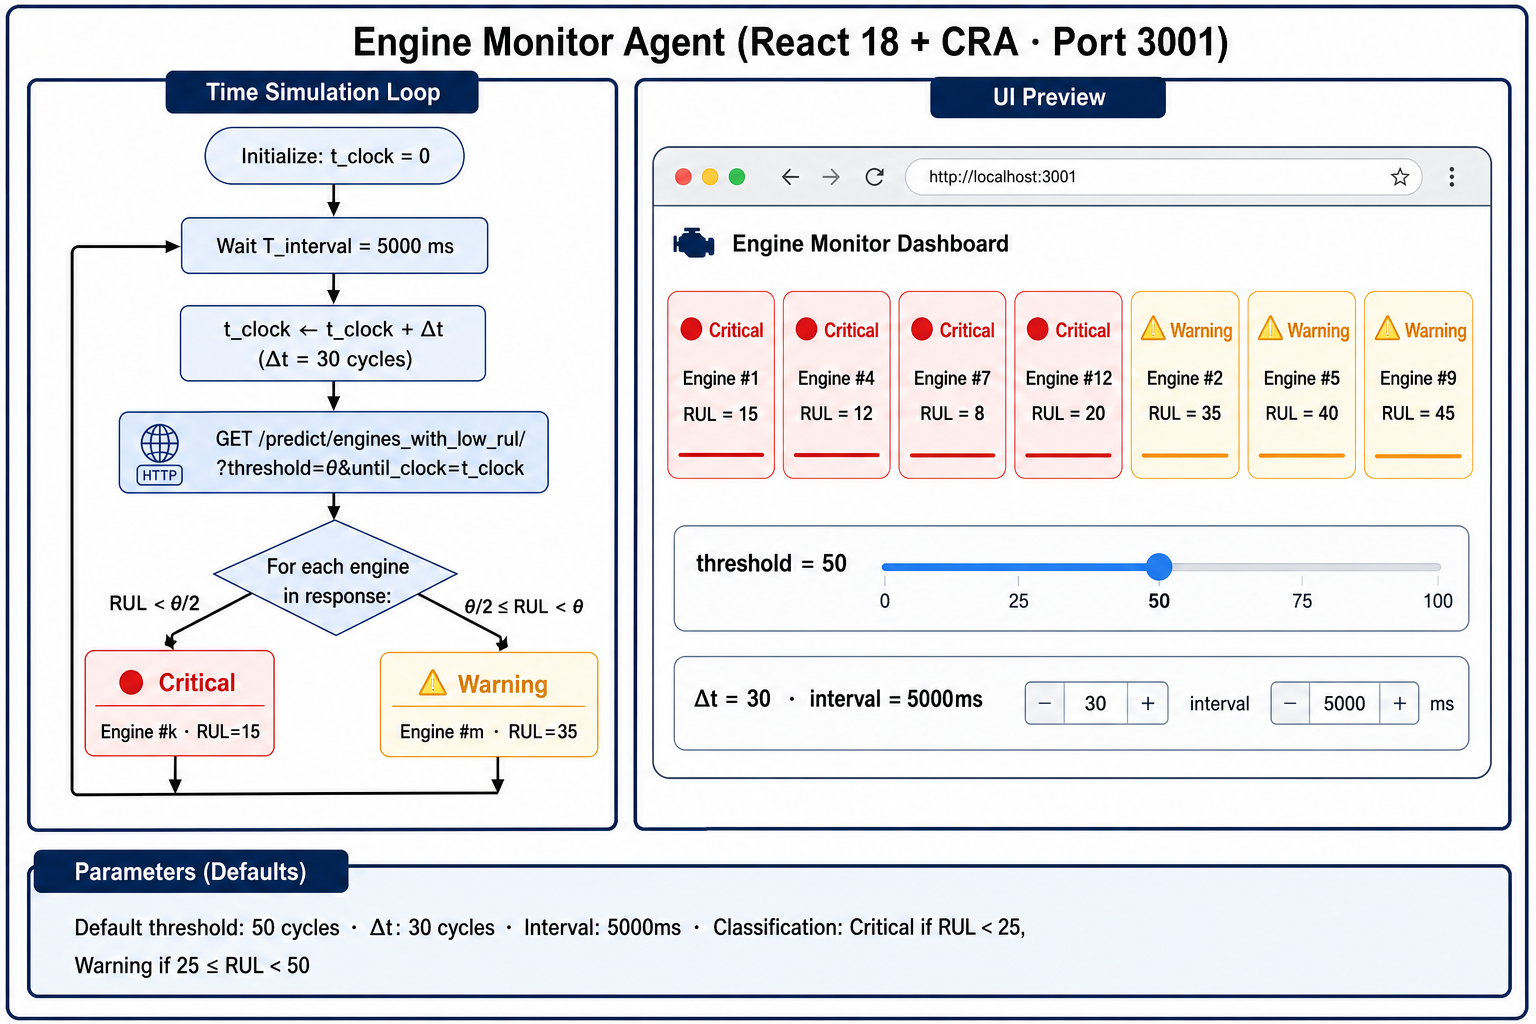
\includegraphics[width=0.95\textwidth]{images/agent_engine_monitor.png}
	\caption{معماری عامل پایش شبه‌بی‌درنگ؛ بخش سمت چپ منطق پیشرفت زمان و فراخوانی API و بخش سمت راست رابط کارت‌محور پایش را نشان می‌دهد}
	\label{fig:impl-monitor-arch}
\end{figure}

\subsection{مؤلفه‌های پایش}

عامل پایش سه مؤلفه اصلی دارد که شامل آستانه ورود به فهرست پایش، گام زمانی شبیه‌سازی و فاصله زمانی میان دو اجرای متوالی حلقه است.

\begin{table}[ht]
	\centering
	\caption{پارامترهای پیش‌فرض عامل پایش}
	\label{tab:monitor-params}
	\begin{tabular}{p{4cm}p{3cm}p{6.5cm}}
		\toprule
		\textbf{پارامتر} & \textbf{مقدار} & \textbf{توضیح} \\
		\midrule
		\lr{threshold} ($\theta$) &
		۵۰ چرخه &
		آستانه ورود به فهرست پایش \\
		
		\addlinespace
		\lr{step} ($\Delta t$) &
		۳۰ چرخه &
		میزان پیشرفت ساعت شبیه‌سازی در هر گام \\
		
		\addlinespace
		\lr{interval} &
		۵۰۰۰ میلی‌ثانیه &
		فاصله زمانی اجرای حلقه \\
		
		\addlinespace
		آستانه بحرانی &
		۲۵ چرخه &
		مرز تفکیک وضعیت هشدار و بحرانی (نصف $\theta$) \\
		\bottomrule
	\end{tabular}
\end{table}

بر اساس این تنظیم، با گذشت زمان، موتوری که \gls{RUL} آن کمتر از ۵۰ چرخه شود وارد فهرست پایش می‌شود و وضعیت آن به صورت \gls{Warning} اعلام می‌شود. پس از گذشت زمان بیشتر،‌ موتور‌ها به آستانه عمر مفید خود نزدیک‌تر می‌شوند و در نتیجه میزان عمر مفید باقیمانده پیش‌بینی شده برای آن‌ها به کمتر از ۲۵ میرسد. در این لحظه وضعیت موتور به صورت \gls{Critical} گزارش می‌شود.

\subsection{رابط کاربری عامل پایش}

رابط کاربری عامل پایش وضعیت موتورهای کم‌عمر را با کارت‌های جداگانه نمایش می‌دهد. استفاده از کدگذاری رنگی باعث می‌شود کاربر بتواند وضعیت موتور‌ها را بدون بررسی جداگانه مقدار \gls{RUL} در هر موتور ارزیابی کند. در تصویر 
\ref{fig:monitor-ui-on}
این کارت‌ها قابل مشاهده هستند. همچنین امکان تنظیم گام زمانی و دوره تکرار حلقه در رابط کاربری فراهم شده است.

\begin{figure}[H]
	\centering
	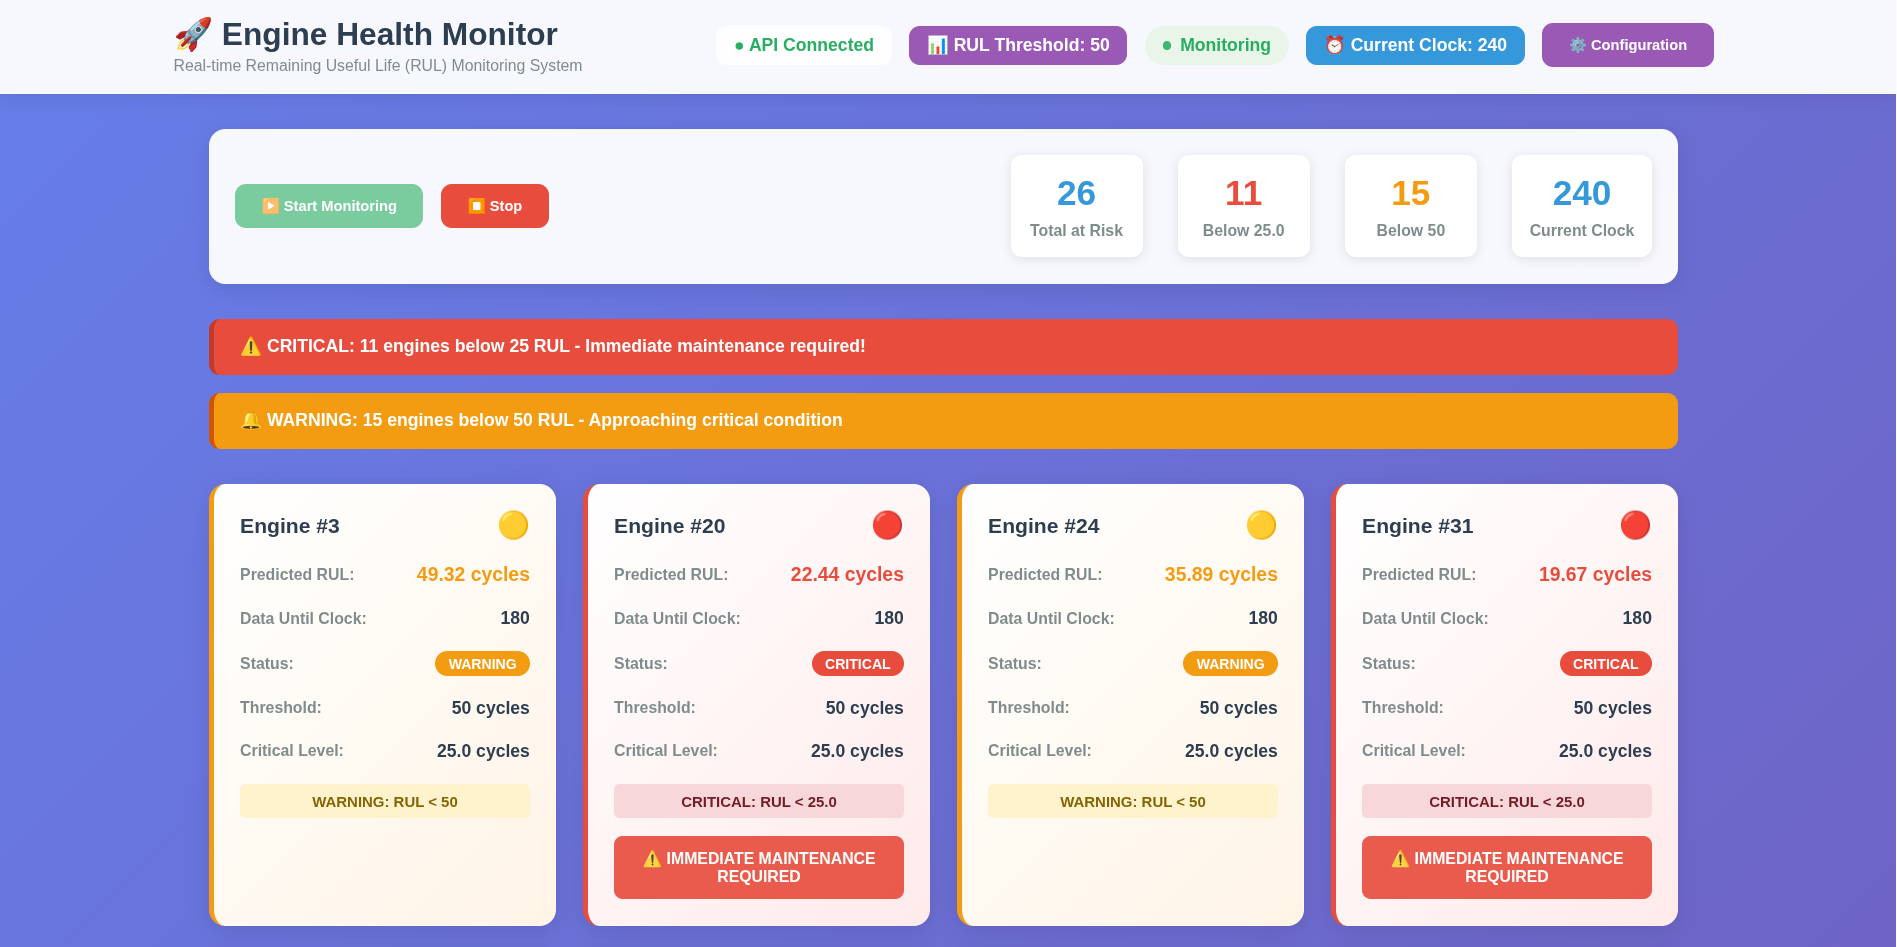
\includegraphics[width=0.92\textwidth]{images/monitor-agent.png}
	\caption{رابط عامل پایش پس از فعال شدن ناوگان؛ کارت‌های هشدار و بحرانی بر اساس مقدار RUL نمایش داده می‌شوند}
	\label{fig:monitor-ui-on}
\end{figure}


% -----------------------------------------------------------------------
\section{عامل تابلو وضعیت}
\label{sec:impl-dashboard}

عامل \gls{Dashboard} وظیفه نمایش وضعیت عملیاتی موتورها را بر عهده دارد. برخلاف عامل پایش، این عامل وارد فرایند پیش‌بینی نمی‌شود و صرفاً وضعیت ثبت‌شده در عامل دوقلو را نمایش می‌دهد. در نتیجه، مرز میان منطق تحلیلی و منطق نمایش در این سرویس حفظ شده است.

\begin{figure}[H]
	\centering
	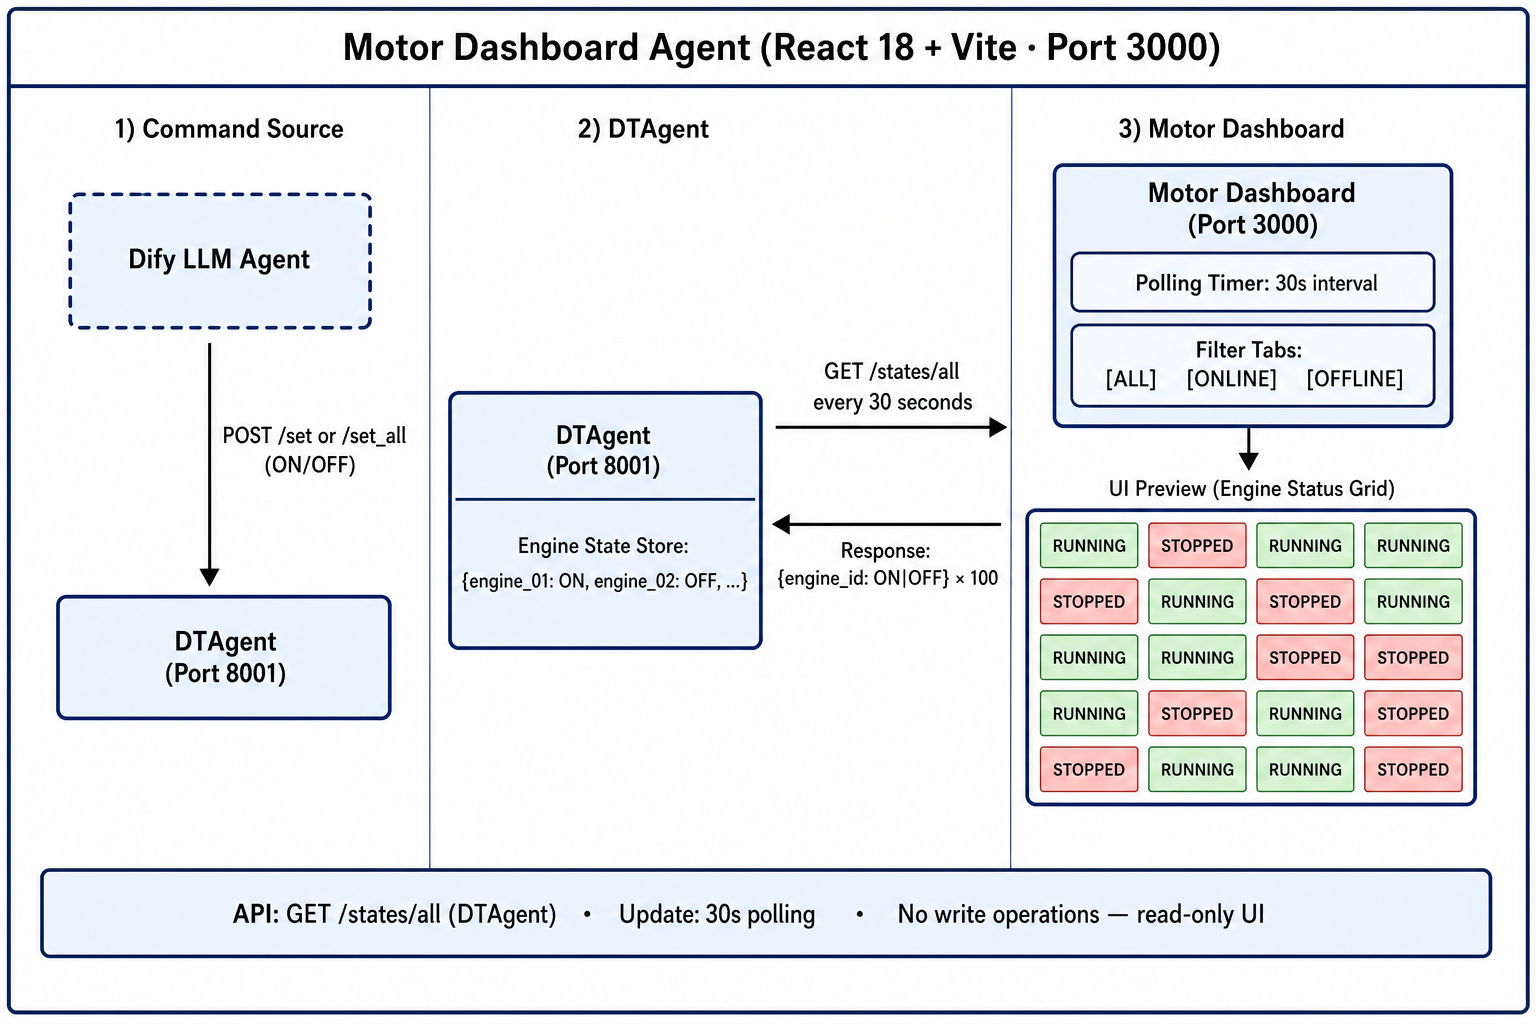
\includegraphics[width=0.90\textwidth]{images/agent_motor_dashboard.png}
	\caption{معماری عامل تابلو وضعیت و جریان یک‌طرفه اطلاعات از عامل دوقلو به رابط نمایش}
	\label{fig:impl-dashboard-arch}
\end{figure}

همانطور که در تصویر 
\ref{fig:impl-dashboard-arch}
قابل مشاهده است، وضعیت موتور‌ها در دوقلوی‌ دیجیتال از طریق عامل مدل‌های زبانی بزرگ می‌تواند تغییر کند و این وضعیت به صورت در لحظه،‌ در عامل تابلو وضعیت قابل مشاهده است.
برای دریافت وضعیت جدید، عامل \gls{Dashboard} از الگوی نظرسنجی دوره‌ای استفاده می‌کند. فاصله پیش‌فرض بین درخواست‌ها ۳۰ ثانیه است. این روش در یک محیط آزمایشگاهی ساده و کم‌هزینه است، اگرچه در یک سامانه صنعتی با نیاز به بازخورد فوری می‌توان از سازوکارهای رویدادمحور مانند \lr{WebSocket} یا \lr{Server-Sent Events} نیز استفاده کرد.

رابط کاربری از سه فیلتر اصلی \lr{ALL}، \lr{ONLINE} و \lr{OFFLINE} استفاده می‌کند. این فیلترها امکان تمرکز کاربر روی بخش مشخصی از موتور‌ها را فراهم می‌کنند. رابط کاربری عامل در تصویر \ref{fig:impl-dashboard-ui} قابل مشاهده است.

\begin{figure}[H]
	\centering
	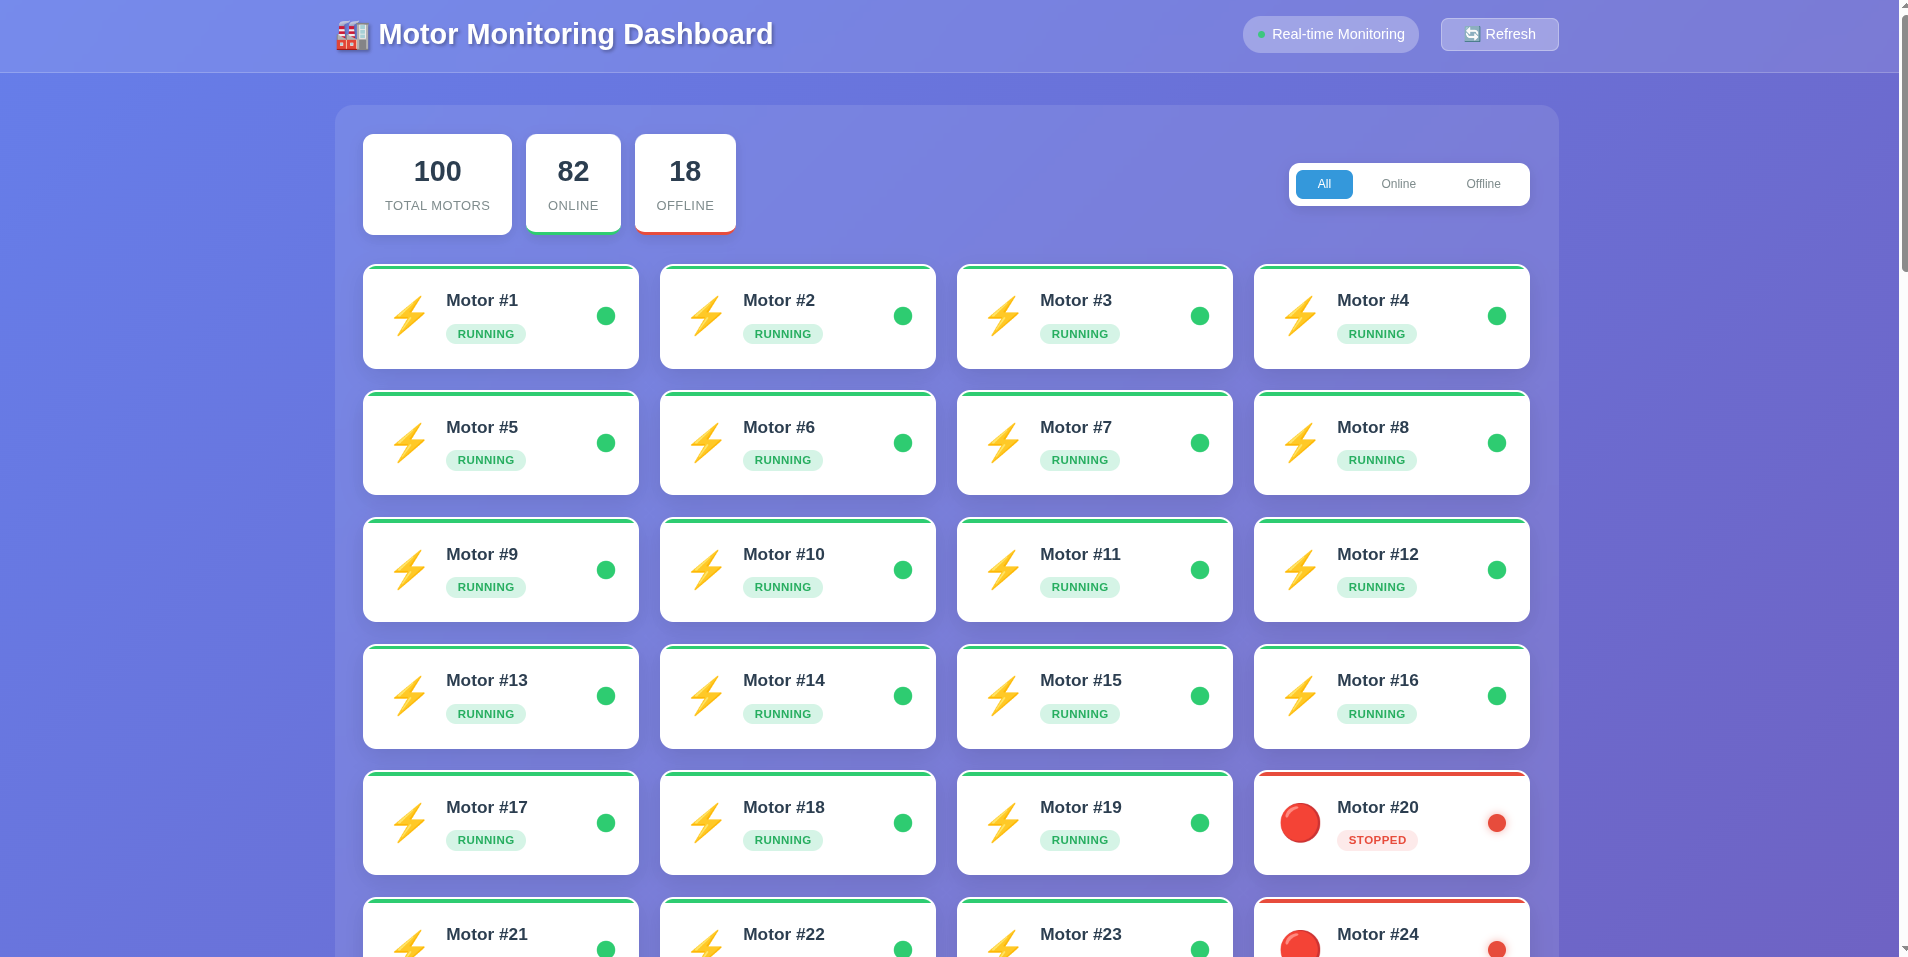
\includegraphics[width=0.90\textwidth]{images/monitor_after_critical_off.png}
	\caption{رابط کاربری عامل 
	تابلو وضعیت
	و فیلتر‌های  \lr{ALL}، \lr{ONLINE} و \lr{OFFLINE}
	}
	\label{fig:impl-dashboard-ui}
\end{figure}

در نتیجه، عامل \gls{Dashboard} را می‌توان یک واسط مشاهده‌گر دانست که وظیفه اصلی آن انتقال وضعیت داخلی دوقلوی دیجیتال به یک نمایش قابل فهم برای کاربر است.

% -----------------------------------------------------------------------
\section{فرایند‌های سرتاسری سامانه}
\label{sec:impl-e2e}

برای ارزیابی انسجام معماری در سطح عملیاتی، دو فرایند اصلی در سامانه اجرا شده است. فرایند اول بر دریافت اطلاعات و پاسخ‌گویی تمرکز دارد و فرایند دوم مسیر تصمیم و کنترل را بررسی می‌کند.

\subsection{فرایند اول: پرس‌وجوی وضعیت موتور}

در این فرایند، کاربر یک پرسش فارسی درباره وضعیت موتور مطرح می‌کند. درخواست ابتدا وارد \gls{Workflow} عامل زبانی می‌شود و نیت مربوط به «وضعیت موتور» تشخیص داده می‌شود. سپس شناسه موتور از متن استخراج و درخواست پیش‌بینی به سرویس مربوط ارسال می‌شود.

عامل پیش‌بینی آخرین پنجره زمانی معتبر موتور را دریافت کرده و مقدار \gls{RUL} را محاسبه می‌کند. پاسخ عددی به صورت ساختاریافته به عامل زبانی بازمی‌گردد و این عامل مقدار عددی را با توجه به آستانه‌های تعریف‌شده تفسیر کرده و به زبان طبیعی فارسی ارائه می‌کند.



\subsection{فرایند دوم: خاموش‌سازی موتورهای در خطر}

در فرایند دوم، اپراتور دستور می‌دهد موتورهای در خطر خاموش شوند. عامل زبانی ابتدا فهرست موتورهایی را که \gls{RUL} آن‌ها از آستانه پایین‌تر است از عامل پیش‌بینی دریافت می‌کند. سپس شناسه این موتورها را به عامل دوقلوی دیجیتال ارسال کرده و فرمان \lr{OFF} اجرا می‌شود.

پس از تغییر وضعیت، عامل \gls{Dashboard} در نظرسنجی بعدی وضعیت جدید موتور را مشاهده می‌کند و کارت موتور از \lr{RUNNING} به \lr{STOPPED} تغییر می‌یابد. هم‌زمان، عامل پایش در اجرای بعدی حلقه خود، موتور خاموش‌شده را دیگر در فهرست موتورهای فعال کم‌عمر قرار نمی‌دهد. این مسیر نشان‌دهنده شکل‌گیری یک حلقه بسته میان پیش‌بینی، تصمیم، کنترل و بازخورد است.


% -----------------------------------------------------------------------
\section{جمع‌بندی}
\label{sec:impl-summary}

در این فصل، معماری پیشنهادی فصل سوم در قالب یک نمونه آزمایشگاهی متشکل از پنج سرویس مستقل پیاده‌سازی شد. عامل دوقلو وظیفه نگهداری داده و وضعیت موتور‌ها را بر عهده گرفت، عامل پیش‌بینی \gls{RUL} را محاسبه کرد، عامل زبانی امکان تعامل طبیعی و ارسال فرمان را فراهم نمود و دو عامل پایش و \gls{Dashboard}، وضعیت سامانه را به کاربر نمایش دادند.

نتیجه پیاده‌سازی نشان می‌دهد که جداسازی مسئولیت‌ها در قالب سرویس‌های مستقل امکان ایجاد یک زنجیره قابل ردیابی از داده تا تصمیم را فراهم کرده است. همچنین، استفاده از پارامتر \lr{until\_clock} امکان شبیه‌سازی جریان زمانی داده‌های \gls{CMAPSS} را بدون نیاز به یک منبع حسگری واقعی فراهم کرده است.

در سطح زیرساخت نیز استقرار کانتینری و استفاده از رابط‌های \lr{REST} امکان اجرای مستقل سرویس‌ها و مدیریت ساده‌تر وابستگی میان آن‌ها را فراهم کرده است. در مقابل، وضعیت درون‌حافظه‌ای، نظرسنجی دوره‌ای و استفاده از داده شبیه‌سازی‌شده از جمله محدودیت‌هایی هستند که هنگام انتقال سامانه از محیط آزمایشگاهی به محیط صنعتی باید برطرف شوند.

در نهایت، اجرای فرایند‌های سرتاسری نشان داد که معماری حاضر صرفاً یک زنجیره پیش‌بینی نیست، بلکه می‌تواند پیش‌بینی را در قالب یک جریان چندعاملی به تصمیم و سپس تغییر وضعیت عملیاتی تبدیل کند. ارزیابی کمی مدل و ارزیابی عملی عملکرد این زنجیره در فصل پنجم ارائه می‌شود.

%*****************************************************************
% chap5.tex
%*****************************************************************

\chapter{ارزیابی و بحث}
\label{chap:eval}

\section{مقدمه}
\label{sec:eval-introduction}

در فصل چهارم، معماری پیشنهادی دوقلوهای دیجیتال چندعاملی از سطح طراحی به یک نمونه آزمایشگاهی قابل اجرا منتقل شد و نحوه پیاده‌سازی عامل دوقلوی دیجیتال، عامل پیش‌بینی عمر مفید باقیمانده، عامل تعامل زبانی، عامل پایش و عامل \gls{Dashboard} تشریح گردید. همچنین نحوه ارتباط میان سرویس‌ها، شبیه‌سازی ورود تدریجی داده‌های مجموعه \gls{CMAPSS}، استقرار سرویس‌ها و اجرای فرایندهای سرتاسری سامانه بررسی شد. ازاین‌رو، هدف فصل حاضر ارزیابی این است که آیا سامانه پیاده‌سازی‌شده توانسته است اهداف اصلی پژوهش را در سه سطح \textbf{پیش‌بینی، یکپارچه‌سازی و تعامل} محقق سازد یا خیر.

بر این اساس، ارزیابی پژوهش در دو سطح انجام می‌شود. در سطح نخست، عملکرد عامل پیش‌بینی \gls{RUL} از طریق مقایسه یک مدل پایه با نسخه نهایی بررسی می‌شود. این ارزیابی با هدف ادعای ارائه بهترین معماری یادگیری عمیق برای مجموعه \gls{CMAPSS} انجام نمی‌شود؛ بلکه هدف آن تعیین این موضوع است که آیا یک مدل پیش‌بینی با عملکرد قابل قبول و رفتار متناسب با نیازهای واقعی صنعت، می‌تواند به عنوان یک بخش تخصصی در معماری چندعاملی مورد استفاده قرار گیرد یا خیر. این تفکیک از اهمیت روش‌شناختی برخوردار است، زیرا در معماری پیشنهادی، مدل یادگیری عمیق تنها یکی از اجزای سامانه محسوب می‌شود و ارزش پژوهش به عملکرد مدل به‌تنهایی محدود نمی‌شود.

در سطح دوم، عملکرد معماری چندعاملی از منظر یکپارچگی سرویس‌ها، پایش شبه‌بی‌درنگ، تعامل با زبان طبیعی، تفسیر خروجی پیش‌بینی و اجرای فرمان‌های کنترلی ارزیابی می‌شود. چنین ارزیابی‌ای با جهت‌گیری پژوهش‌های جدید در زمینه دوقلوهای دیجیتال عامل‌محور نیز هم‌راستا است. در این پژوهش‌ها، هدف از ترکیب دوقلوی دیجیتال و عامل‌های هوشمند، حرکت از یک بازنمایی صرفاً اطلاعاتی به سمت سامانه‌هایی است که بتوانند وضعیت را درک کرده، تصمیم مناسب پیشنهاد دهند و در چارچوب کنترل‌شده در فرایند عملیاتی مشارکت کنند \cite{lopez2024madtwin,puiu2025synergies,nicoletti2026humanagentic}.

بنابراین، پرسش اصلی این فصل چنین بیان می‌شود: آیا معماری پیشنهادی می‌تواند یک مدل پیش‌بینی \gls{RUL} را به یک جزء قابل استفاده در یک سامانه چندعاملی تبدیل کند که علاوه بر تخمین عمر مفید، امکان پایش، توضیح وضعیت، تعامل طبیعی و اعمال فرمان را نیز فراهم آورد؟ پاسخ به این پرسش، بر اساس نتایج کمی مدل، مطالعات موردی عامل زبانی، بررسی حلقه بسته تصمیم و مقایسه با پژوهش‌های مرتبط ارائه خواهد شد.

\section{راهبرد ارزیابی}
\label{sec:evaluation-strategy}

راهبرد ارزیابی پژوهش با توجه به ماهیت چندلایه سامانه طراحی شده است. از آنجا که معماری پیشنهادی از چند مؤلفه مستقل تشکیل شده است، ارزیابی صرفاً بر یک معیار عددی مانند \lr{MAE} نمی‌تواند میزان موفقیت کل سامانه را نشان دهد. به همین دلیل، چهار بعد اصلی برای ارزیابی در نظر گرفته شده است:

\begin{enumerate}
	\item ارزیابی عملکرد پیش‌بینی \gls{RUL}؛
	\item ارزیابی رفتار محافظه‌کارانه مدل در برابر خطای بیش‌برآورد؛
	\item ارزیابی قابلیت تعامل و تفسیر خروجی توسط عامل زبانی؛
	\item ارزیابی یکپارچگی معماری از طریق اجرای حلقه بسته پیش‌بینی، تصمیم، کنترل و بازخورد.
\end{enumerate}

این رویکرد با روند جدید پژوهش در زمینه نگهداری پیش‌بینانه و کاربرد در صنعت نیز سازگار است. پژوهش‌های جدید \gls{RUL} نشان می‌دهند که ارزیابی مدل تنها بر اساس خطای نقطه‌ای کافی نیست و عواملی مانند عدم‌قطعیت، قابلیت اعتماد پیش‌بینی و هزینه نامتقارن خطاها باید در نظر گرفته شوند \cite{diao2026reliable,hatipoglu2025matrix}. به‌خصوص در تجهیزات صنعتی، بیش‌برآورد عمر مفید می‌تواند از نظر عملیاتی خطرناک‌تر از کم‌برآورد آن باشد؛ زیرا کم‌برآورد عمدتاً به بازرسی یا نگهداری زودتر منجر می‌شود، درحالی‌که بیش‌برآورد می‌تواند موجب ادامه بهره‌برداری از تجهیزی شود که به انتهای عمر خود نزدیک شده است.

از این منظر، هدف مدل پیش‌بینی در این پژوهش کمینه‌سازی کورکورانه خطای عددی نیست، بلکه تولید پیش‌بینی‌ای است که در زنجیره تصمیم‌گیری سامانه بتوان به آن تکیه کرد. این موضوع یکی از تفاوت‌های مهم میان رویکرد حاضر و پژوهش‌هایی است که مسئله CMAPSS را صرفاً به عنوان یک مسئله رقابت برای کاهش \lr{MAE} یا \lr{RMSE} در نظر می‌گیرند.

\section{تنظیم آزمایش‌ها}
\label{sec:experiment-setup}

\subsection{مجموعه داده و پروتکل ارزیابی}

تمام آزمایش‌های کمی این پژوهش بر روی زیرمجموعه \lr{FD001} مجموعه داده \gls{CMAPSS} انجام شده است. انتخاب \lr{FD001} به این دلیل صورت گرفته است که این زیرمجموعه دارای یک شرایط عملیاتی و یک حالت خرابی است و در نتیجه امکان بررسی رفتار مدل بدون ورود هم‌زمان به پیچیدگی ناشی از چندین شرایط عملیاتی فراهم می‌شود.

مجموعه آموزشی همانطور که در جدول 
\ref{tab:eval-data}
مشخص شده،
شامل ۱۰۰ موتور و ۲۰٬۶۳۱ رکورد حسگر و مجموعه آزمون شامل ۱۰۰ موتور و ۱۳٬۰۹۶ رکورد است. برای هر موتور آزمون، داده‌ها تا یک نقطه زمانی مشخص در اختیار سامانه قرار گرفته و هدف، تخمین عمر مفید باقیمانده موتور در همان نقطه است. این ساختار با ماهیت کاربردی پیش‌بینی خرابی سازگار است؛ زیرا در یک کاربرد واقعی نیز سامانه باید بر اساس اطلاعات موجود تا زمان جاری، وضعیت آینده تجهیز را تخمین بزند.

\begin{table}[ht]
	\centering
	\caption{مشخصات مجموعه داده مورد استفاده در ارزیابی}
	\label{tab:eval-data}
	\begin{tabular}{p{5cm}p{6cm}}
		\toprule
		\textbf{مشخصه} & \textbf{مقدار} \\
		\midrule
		زیرمجموعه & \lr{FD001} \\
		شرایط عملیاتی & یک شرایط عملیاتی \\
		حالت خرابی & یک حالت خرابی \\
		تعداد موتورهای آموزش & ۱۰۰ \\
		تعداد موتورهای آزمون & ۱۰۰ \\
		تعداد رکوردهای آموزش & ۲۰٬۶۳۱ \\
		تعداد رکوردهای آزمون & ۱۳٬۰۹۶ \\
		طول پنجره زمانی & ۵۰ چرخه \\
		تعداد ویژگی‌ها & ۱۴ ویژگی در هر گام زمانی \\
		\bottomrule
	\end{tabular}
\end{table}

انتخاب \lr{FD001} را نباید به عنوان ادعای تعمیم‌یافتن نتایج مدل به تمام شرایط عملیاتی تفسیر کرد. این انتخاب صرفاً یک نقطه شروع کنترل‌شده برای ارزیابی معماری است. پژوهش‌های جدید نیز نشان داده‌اند که تغییر شرایط عملیاتی و انتقال بین زیرمجموعه‌های مختلف CMAPSS می‌تواند مسئله پیش‌بینی \gls{RUL} را به‌طور قابل توجهی دشوارتر کند \cite{diao2026reliable,song2026degradation}.

\subsection{مدل‌های مورد مقایسه}

برای ارزیابی نقش تغییرات انجام‌شده در مدل پیش‌بینی، دو پیکربندی در نظر گرفته شده است. مدل نخست به عنوان \gls{Baseline}، از یک معماری دو لایه LSTM، تابع زیان MSE و بدون سازوکار توجه استفاده می‌کند. هدف از این مدل، ایجاد یک مرجع ساده و قابل تکرار برای ارزیابی نسخه نهایی است.

مدل دوم که با عنوان \lr{V2} مشخص می‌شود، از همان ساختار اصلی LSTM استفاده می‌کند، اما با افزودن لایه توجه و جایگزینی MSE با تابع زیان \lr{Pinball} در ضریب $\tau=0.125$ آموزش داده شده است.

\begin{table}[ht]
	\centering
	\caption{پیکربندی مدل پایه و مدل نهایی}
	\label{tab:models-evaluation}
	\begin{tabular}{p{4cm}p{4cm}p{3cm}p{3cm}}
		\toprule
		\textbf{مدل} & \textbf{معماری} & \textbf{تابع زیان} & \textbf{لایه توجه} \\
		\midrule
		\lr{Baseline} & LSTM دو لایه & MSE & خیر \\
		\lr{V2} & LSTM دو لایه + Attention & Pinball $(\tau=0.125)$ & بله \\
		\bottomrule
	\end{tabular}
\end{table}

تأکید می‌شود که این مقایسه با هدف جست‌وجوی فضای گسترده معماری‌های یادگیری عمیق یا اثبات برتری LSTM نسبت به مدل‌های دیگر انجام نشده است. در واقع، مدل پیش‌بینی در این پژوهش یک مؤلفه تخصصی از معماری است و نه موضوع اصلی پژوهش. این تصمیم با هدف معماری سازگار است. در صورتی که مدل پیش‌بینی در آینده با یک مدل \gls{Transformer}، مدل احتمالاتی یا روش دیگری جایگزین شود، سایر اجزای معماری همچنان قابل استفاده خواهند بود.

\section{ارزیابی مدل پیش‌بینی عمر مفید باقیمانده}
\label{sec:rul-results}

\subsection{معیارهای ارزیابی}

برای ارزیابی مدل‌ها از معیارهای \lr{MAE}، \lr{RMSE}، $R^2$ و نسبت کم‌برآورد استفاده شده است. \lr{MAE} میانگین قدر مطلق خطا را نشان می‌دهد و تصویری مستقیم از میزان خطای پیش‌بینی ارائه می‌کند. \lr{RMSE} نسبت به خطاهای بزرگ حساس‌تر است و بنابراین می‌تواند برای بررسی وجود خطاهای شدید مفید باشد. همچنین $R^2$ میزان توانایی مدل در توضیح تغییرات مقدار واقعی RUL را اندازه‌گیری می‌کند.

با این حال، در مسئله حاضر نسبت کم‌برآورد نیز اهمیت ویژه‌ای دارد. این معیار به صورت رابطه 
\ref{eq:under-stimate}
تعریف می‌شود.

\begin{equation} \label{eq:under-stimate}
	r_{\mathrm{under}}
	=
	\frac{
		\sum_{i=1}^{N}
		\mathbb{I}(\hat{y}_i < y_i)
	}{
		N
	},
\end{equation}

که در آن $\hat{y}_i$ مقدار پیش‌بینی‌شده و $y_i$ مقدار واقعی \gls{RUL} است.

این معیار نشان می‌دهد چه نسبتی از پیش‌بینی‌ها کمتر از عمر واقعی قرار گرفته‌اند. افزایش این نسبت لزوماً به معنای بهتر شدن مدل از نظر معیارهای عمومی نیست؛ بلکه در این پژوهش به عنوان یک ویژگی ایمنی مطلوب تفسیر می‌شود. پژوهش‌های جدید نیز به اهمیت پیش‌بینی ریسک‌آگاه و لحاظ عدم‌قطعیت در تصمیم‌های نگهداری اشاره کرده‌اند \cite{diao2026reliable,hatipoglu2025matrix}.

\subsection{نتایج کمی مدل‌ها}

نتایج حاصل از مجموعه آزمون در جدول \ref{tab:lstm-results-final} ارائه شده است.

\begin{table}[ht]
	\centering
	\caption{مقایسه عملکرد مدل پایه و مدل \lr{V2} روی \lr{FD001}}
	\label{tab:lstm-results-final}
	\begin{tabular}{p{4cm}p{3cm}p{3cm}p{3cm}}
		\toprule
		\textbf{معیار} & \textbf{\lr{Baseline}} & \textbf{\lr{V2}} & \textbf{تغییر} \\
		\midrule
		\lr{MAE} & ۱۷٫۵۶ & \textbf{۱۷٫۲۱} & بهبود محدود \\
		$R^2$ & ۰٫۲۴ & \textbf{۰٫۷۱} & بهبود قابل توجه \\
		\lr{RMSE} & --- & \textbf{۲۲٫۹۲} & --- \\
		نسبت کم‌برآورد & ۴۷\% & \textbf{۸۷\%} & افزایش هدفمند \\
		\bottomrule
	\end{tabular}
\end{table}

نتایج نشان می‌دهد که تغییر معماری و تابع زیان اثر یکسانی بر تمام معیارها نداشته است. مقدار \lr{MAE} از ۱۷٫۵۶ به ۱۷٫۲۱ کاهش یافته است که اگرچه بهبود محسوسی نیست، اما نشان می‌دهد افزودن سازوکار توجه و تغییر تابع زیان موجب تخریب عملکرد کلی مدل نشده است. در مقابل، افزایش $R^2$ از ۰٫۲۴ به ۰٫۷۱ نشان می‌دهد که نسخه نهایی توانسته است ساختار تغییرات \gls{RUL} را بهتر از مدل پایه دنبال کند. این نتیجه که در شکل 
\ref{tab:lstm-results-final}
نیز قابل مشاهده است، اهمیت توجه به چند معیار را نشان می‌دهد. اگر ارزیابی تنها بر اساس MAE انجام می‌شد، تفاوت میان دو مدل نسبتاً کوچک به نظر می‌رسید؛ درحالی‌که $R^2$ نشان می‌دهد رفتار مدل نهایی از نظر دنبال‌کردن روند تغییرات RUL تفاوت معناداری با مدل پایه دارد.

\begin{figure}[H]
	\centering
	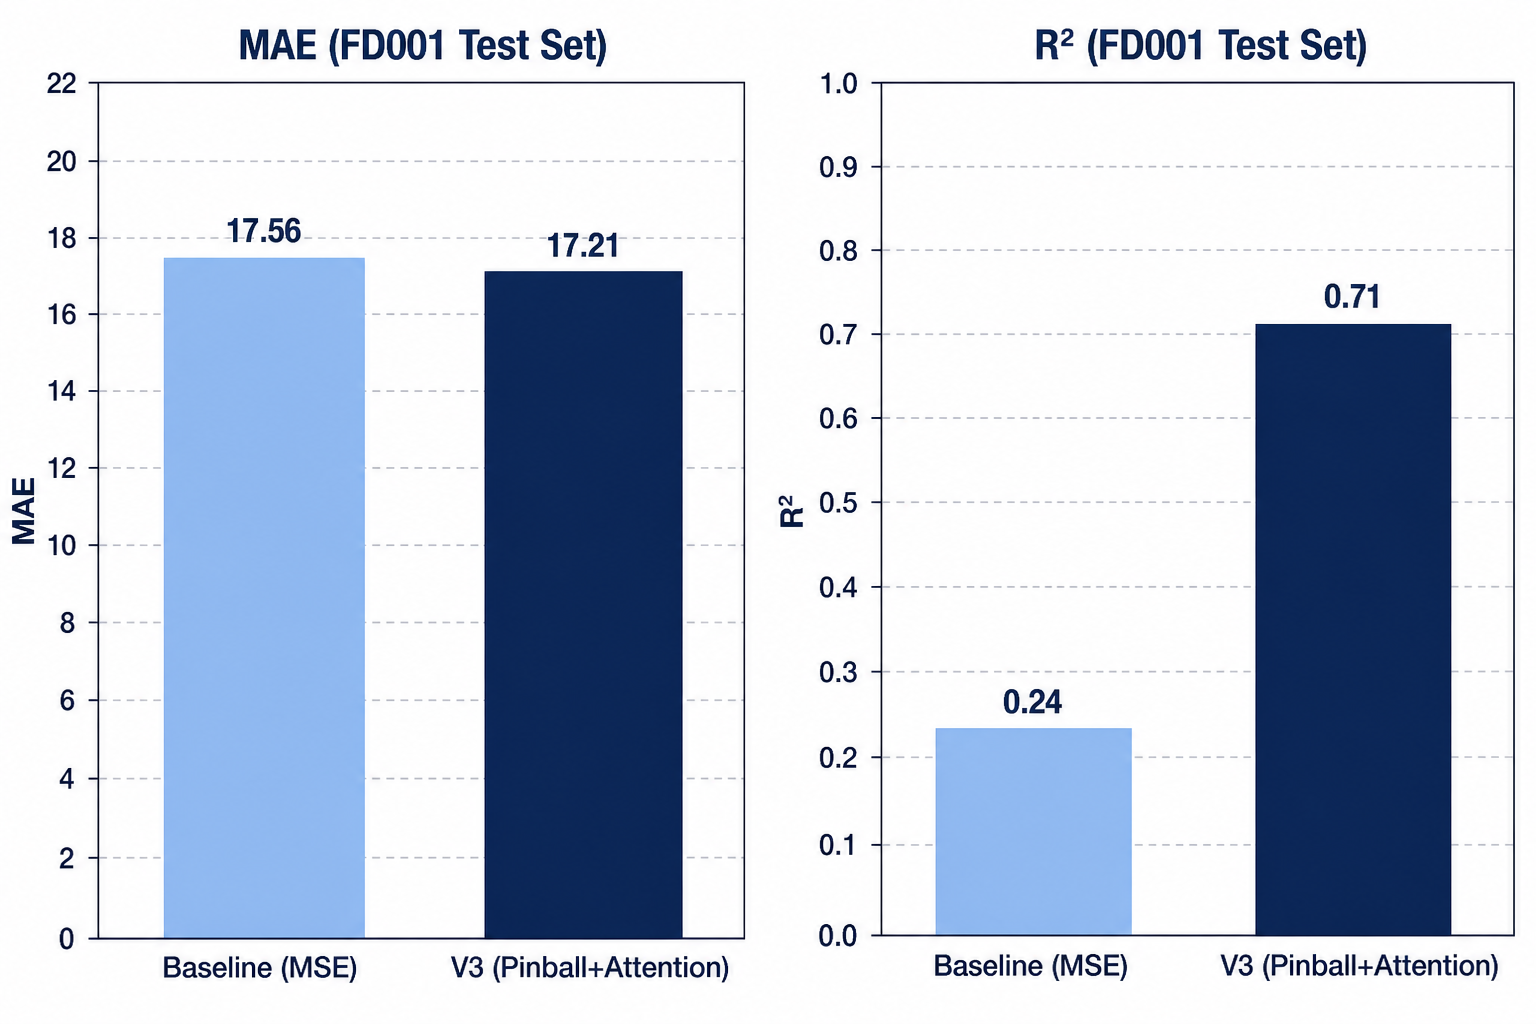
\includegraphics[width=0.82\textwidth]{images/metric_comparison.png}
	\caption{مقایسه معیارهای کمی مدل پایه و مدل \lr{V2}}
	\label{fig:metric-comparison-final}
\end{figure}

بنابراین، نتیجه این آزمایش نباید چنین تفسیر شود که مدل \lr{V2} بهترین مدل ممکن برای CMAPSS است. نتیجه مورد انتظار آن است که مدل انتخاب‌شده، با پیچیدگی نسبتاً محدود، عملکرد کافی برای ایفای نقش یک سرویس پیش‌بینی در معماری پیشنهادی به دست آورده است. این موضوع برای هدف پژوهش اهمیت بیشتری دارد، زیرا خروجی این مدل مستقیماً در عامل پایش، عامل زبان طبیعی و تصمیم‌های عملیاتی استفاده می‌شود.

\subsection{رفتار آموزشی مدل}

نتایج آموزش مدل \lr{V2} در ۶۰ دوره در شکل \ref{fig:train-curves-ch5} نشان داده شده است. روند کلی منحنی‌های آموزش و اعتبارسنجی نشان می‌دهد که مدل در دوره‌های ابتدایی به سرعت به سمت ناحیه مناسب حرکت کرده و پس از حدود دوره بیستم، سرعت بهبود کاهش یافته است.

\begin{figure}[H]
	\centering
	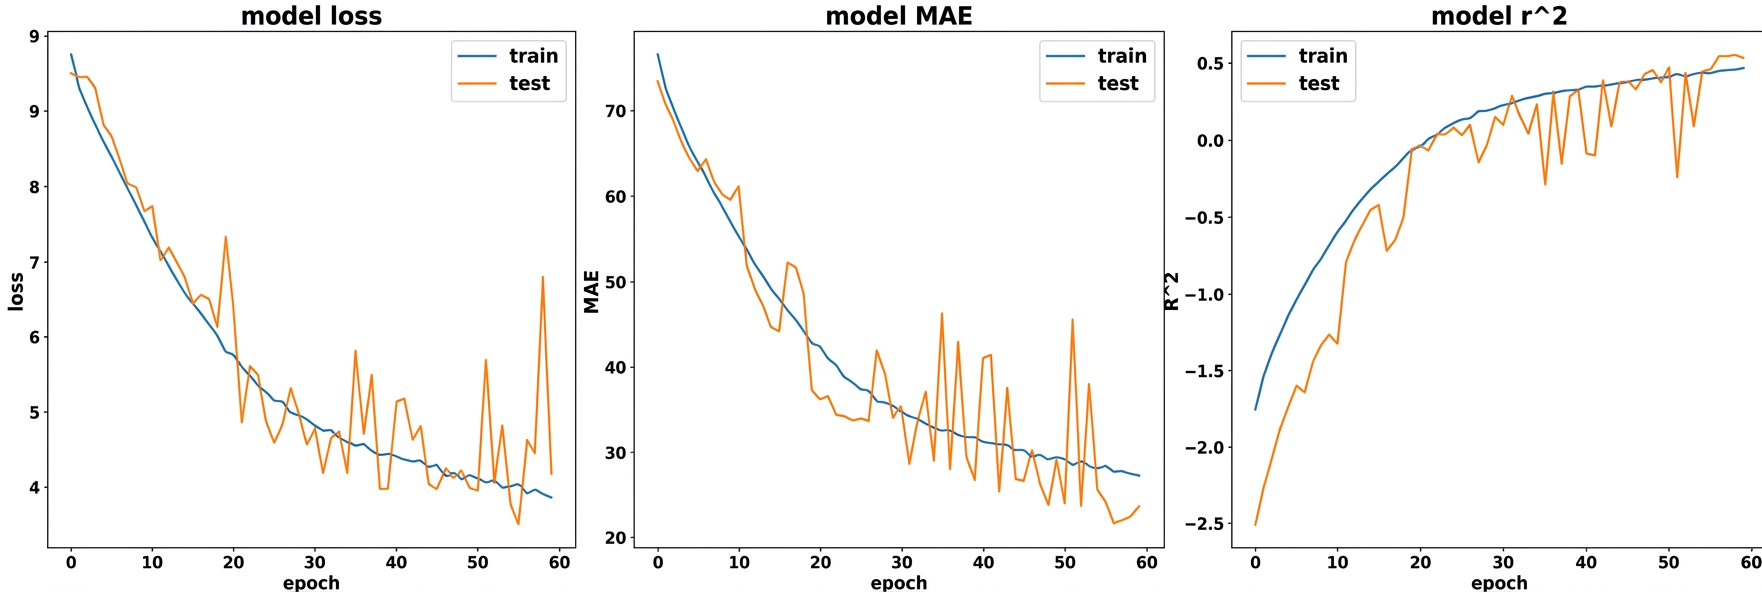
\includegraphics[width=1.0\textwidth]{images/plot-32.png}
	\caption{منحنی‌های آموزش مدل \lr{V2} در ۶۰ دوره}
	\label{fig:train-curves-ch5}
\end{figure}

در پایان آموزش، مقدار \lr{MAE} آموزش برابر ۲۷٫۱۷ و مقدار آن در اعتبارسنجی برابر ۲۳٫۵۷ بوده است. همچنین $R^2$ آموزش ۰٫۴۶ و $R^2$ اعتبارسنجی ۰٫۵۳ گزارش شده است. نبود شکاف بسیار بزرگ میان آموزش و اعتبارسنجی، دست‌کم در این آزمایش، نشانه‌ای از بیش‌برازش شدید ندارد.

با این حال، نباید از این نتیجه‌گیری فراتر رفت و آن را به معنای اثبات تعمیم کامل مدل دانست. آزمون واقعی تعمیم مدل، عملکرد آن روی موتورهای دیده‌نشده مجموعه آزمون است و تعمیم به شرایط عملیاتی جدید یا زیرمجموعه‌های دیگر CMAPSS به آزمایش‌های جداگانه نیاز دارد.

\subsection{تحلیل کم‌برآورد و انتخاب تابع زیان}

یکی از ویژگی‌های اصلی طراحی مدل نهایی، استفاده از تابع زیان \lr{Pinball} با $\tau=0.125$ است. انگیزه این انتخاب، ایجاد یک مدل صرفاً دقیق‌تر از نظر میانگین خطا نبوده است، بلکه هدف، ایجاد گرایش کنترل‌شده به سمت کم‌برآورد \gls{RUL} بوده است.


در آزمایش حاضر و همانطور که در نمودار 
\ref{fig:underestimation-final}
قابل مشاهده است، نسبت کم‌برآورد از ۰٫۴۷ در مدل پایه به ۰٫۸۷ در مدل \lr{V2} افزایش یافته است.

\begin{figure}[H]
	\centering
	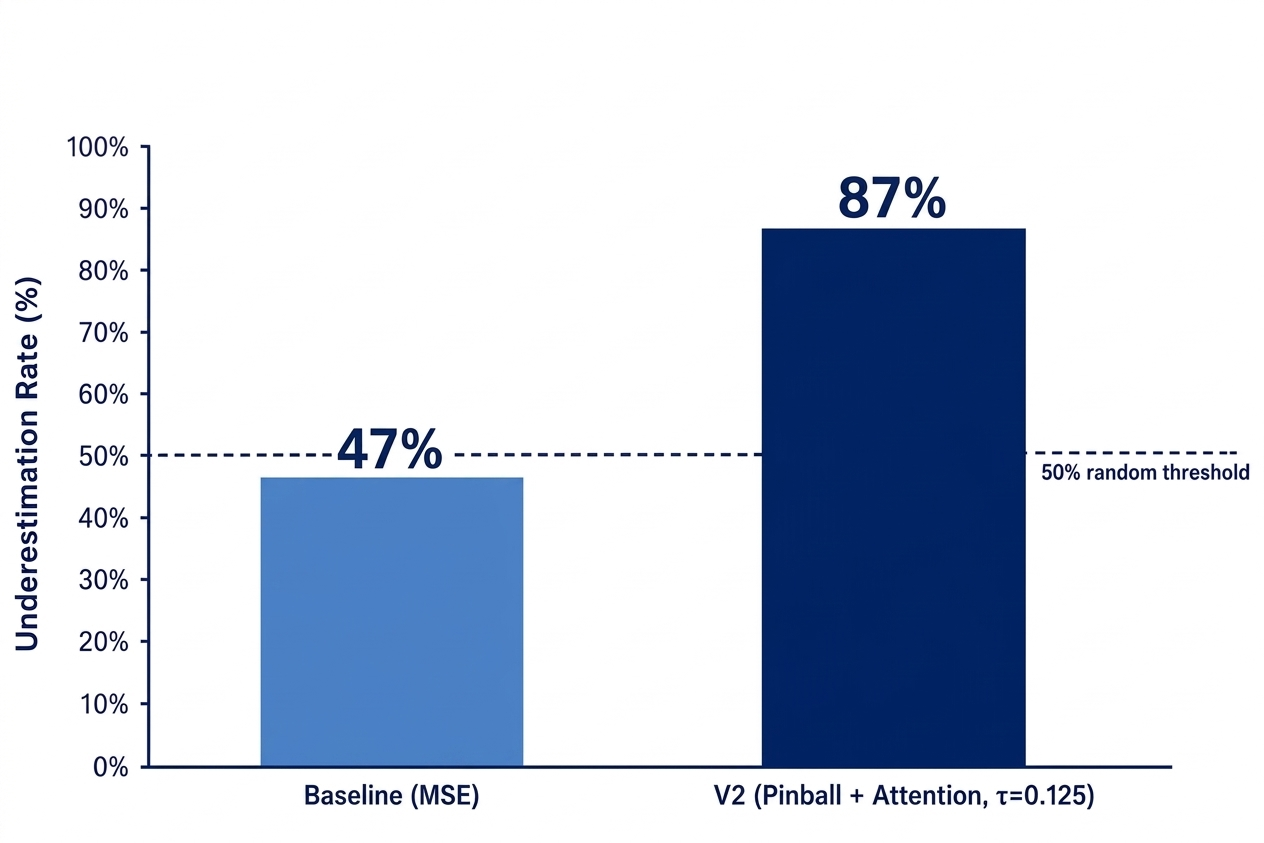
\includegraphics[width=0.90\textwidth]{images/underestimation_comparison2.png}
	\caption{مقایسه نسبت کم‌برآورد مدل پایه و مدل \lr{V2}}
	\label{fig:underestimation-final}
\end{figure}

این افزایش باید به عنوان یک \textbf{ویژگی طراحی‌شده} تفسیر شود، نه صرفاً یک بهبود آماری. در واقع، مدل نهایی آگاهانه از بخشی از دقت بی‌طرفانه فاصله گرفته تا رفتار محافظه‌کارانه‌تری در زنجیره تصمیم ایجاد کند. این ویژگی برای معماری پیشنهادی اهمیت دارد، زیرا خروجی مدل مستقیماً به عامل پایش منتقل شده و می‌تواند وضعیت موتور را از عادی به هشدار یا بحرانی تغییر دهد.

در نتیجه، تابع زیان انتخاب‌شده یکی از نقاطی است که در آن نیاز صنعتی مستقیماً وارد طراحی مدل شده است. به عبارت دیگر، مدل برای یک مسئله انتزاعی پیش‌بینی عددی طراحی نشده، بلکه برای قرار گرفتن در یک سامانه تصمیم‌یار نگهداری طراحی شده است.

\subsection{مقایسه پیش‌بینی و مقدار واقعی}

نمودار \ref{fig:pred-vs-actual-final} مقادیر پیش‌بینی‌شده و واقعی RUL را برای موتورهای آزمون نشان می‌دهد.

\begin{figure}[H]
	\centering
	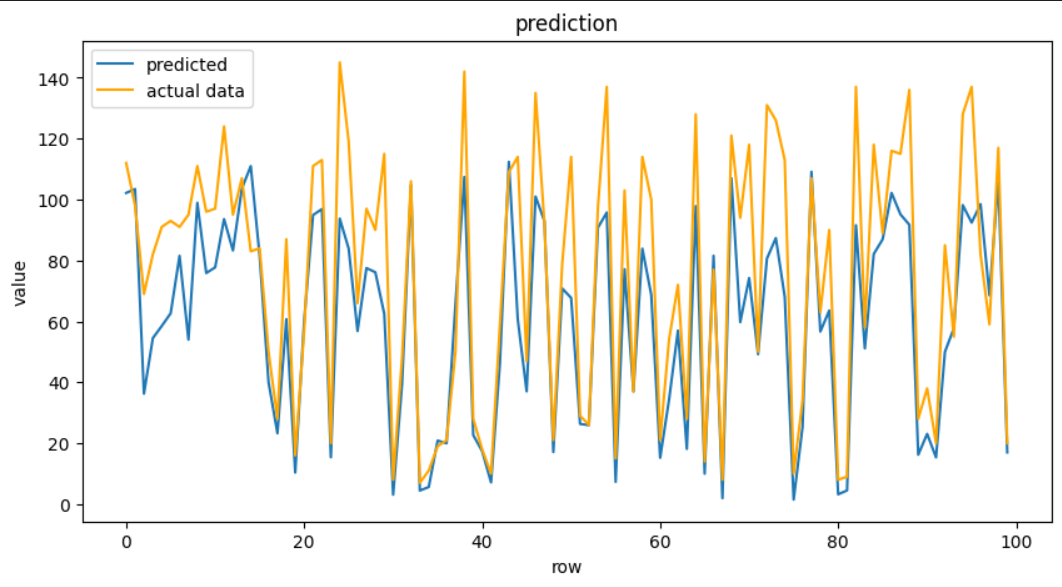
\includegraphics[width=0.92\textwidth]{images/pred_vs_actual_v3-plot.png}
	\caption{مقایسه مقادیر پیش‌بینی‌شده و واقعی RUL برای موتورهای آزمون}
	\label{fig:pred-vs-actual-final}
\end{figure}

قرار گرفتن بخش قابل توجهی از پیش‌بینی‌ها در پایین‌تر از مقادیر واقعی با هدف استفاده از تابع زیان نامتقارن سازگار است. در نتیجه، شکل حاصل علاوه بر آنکه عملکرد مدل را نمایش می‌دهد، رفتار طراحی‌شده آن را نیز آشکار می‌کند.

البته کم‌برآورد بیش از حد نیز می‌تواند هزینه عملیاتی ایجاد کند. اگر عمر موتور به صورت دائمی کمتر از مقدار واقعی برآورد شود، ممکن است بازرسی‌ها و تعمیرات غیرضروری افزایش یابند. بنابراین، هدف کاربردی یک سامانه صنعتی، دستیابی به کم‌برآورد حداکثری نیست؛ بلکه دستیابی به نقطه‌ای مناسب میان ایمنی، هزینه نگهداری و عدم‌قطعیت است. مقدار $\tau=0.125$ در این پژوهش به عنوان یک انتخاب اولیه و محافظه‌کارانه ارزیابی شده و نه به عنوان مقدار بهینه عمومی برای همه انواع موتورها. بنا به نوع و جنس موجودیت‌ها در لایه فیزیکی و میزان خسارتی که خرابی آن‌ها به بار می‌آورند، می‌توان ضریب $tau$ را تغییر داد.

\section{جایگاه مدل LSTM در معماری پیشنهادی}
\label{sec:lstm-role}

نتایج این بخش نشان می‌دهد که مدل LSTM انتخاب‌شده توانسته است یک سرویس پیش‌بینی قابل استفاده برای سامانه فراهم کند. با این ‌حال، لازم است جایگاه این نتیجه در کل پژوهش به‌درستی مشخص شود.

هدف پژوهش حاضر طراحی یک معماری جدید برای رقابت مستقیم با تمامی مدل‌های پیشرفته پیش‌بینی \gls{RUL} نیست. LSTM در اینجا به عنوان یک مدل تخصصی پیش‌بینی در عامل پیش‌بینی قرار گرفته است. این جداسازی از نظر معماری اهمیت دارد، زیرا مدل پیش‌بینی می‌تواند در آینده با مدل‌های دیگری جایگزین شود، بدون آنکه عامل دوقلو، عامل پایش، عامل زبانی یا واسط کاربر نیازمند بازطراحی اساسی باشند.

این ویژگی یکی از مزایای اصلی معماری چندعاملی است. در سیستم‌های چندعاملی، مسئولیت‌ها میان عامل‌های تخصصی توزیع می‌شوند و هر عامل می‌تواند وظیفه مشخصی را انجام دهد \cite{dorri2018multiagent,pretel2022masdt,lopez2024madtwin}. از این منظر، مدل LSTM بخشی از معماری است و نه خود معماری.


در مقایسه با این مسیر، سهم مدل پیش‌بینی حاضر در آن است که یک مدل نسبتاً ساده و قابل پیاده‌سازی را به عنوان جزء محاسباتی معماری چندعاملی به کار گرفته و خروجی آن را در یک زنجیره کامل داده، پیش‌بینی، پایش، توضیح و کنترل قرار داده است. همچنین استفاده واقعی در صنعت را نیز در نظر گرفته و نسبت کم‌برآورد‌ها را افزایش داده است.

\section{ارزیابی عامل تعامل زبانی}
\label{sec:llm-evaluation}

یکی از اهداف اصلی معماری پیشنهادی، ایجاد یک رابط طبیعی میان کاربر و دوقلوی دیجیتال است. همان‌طور که در فصل چهارم توضیح داده شد، عامل زبانی، خود وظیفه تولید مقدار \gls{RUL} را بر عهده ندارد؛ بلکه خروجی عددی عامل پیش‌بینی را دریافت کرده، وضعیت موتور را تفسیر کرده و در صورت نیاز فرمان مناسب را به عامل دوقلو ارسال می‌کند. این جداسازی برای جلوگیری از مخلوط شدن وظیفه استنتاج عددی با وظیفه تعامل انسانی اهمیت دارد.

برای ارزیابی عامل زبانی، شش فرایند کاربردی اجرا شده است. این فرایند‌ها شامل معرفی قابلیت‌های عامل، پرس‌وجوی وضعیت موتور سالم، پرس‌وجوی وضعیت موتور بحرانی، خاموش‌کردن همه موتورها، روشن‌کردن همه موتورها و خاموش‌کردن موتورهای در معرض خطر بوده‌اند.

\begin{table}[ht]
	\centering
	\caption{فرایند‌های ارزیابی عامل تعامل زبانی}
	\label{tab:llm-case-final}
	\begin{tabular}{p{0.6cm}p{3.3cm}p{5cm}p{3cm}}
		\toprule
		\textbf{\#} & \textbf{فرایند} & \textbf{هدف} & \textbf{نتیجه} \\
		\midrule
		۱ & معرفی عامل & بررسی دسترسی به قابلیت‌ها & صحیح \\
		۲ & پرس‌وجوی موتور سالم & دریافت و تفسیر \gls{RUL} & صحیح \\
		۳ & پرس‌وجوی موتور بحرانی & تشخیص وضعیت و ارائه دلیل & صحیح \\
		۴ & خاموش‌کردن همه موتورها & اجرای فرمان کنترلی & موفق \\
		۵ & روشن‌کردن همه موتورها & بازگرداندن وضعیت عملیاتی & موفق \\
		۶ & خاموش‌کردن موتورهای در خطر & ترکیب پیش‌بینی و کنترل & موفق \\
		\bottomrule
	\end{tabular}
\end{table}

در آزمایش انجام‌شده، ۳۰ درخواست مختلف برای عامل زبانی مورد بررسی قرار گرفته و نرخ موفقیت درخواست‌ها ۱۰۰ درصد گزارش شده است. منظور از موفقیت در اینجا، اجرای صحیح مسیر تعریف‌شده در گردش‌کار، دریافت داده مورد انتظار و تولید پاسخ یا اعمال فرمان مورد انتظار است؛ بنابراین این عدد نباید با معیارهایی مانند دقت مدل زبانی عمومی یا صحت آزاد و نامحدود استدلال مقایسه شود.

\subsection{تفسیر خروجی پیش‌بینی توسط عامل زبانی}

یکی از کاربردهای مهم عامل زبانی، تبدیل مقدار عددی \gls{RUL} به اطلاعات قابل فهم برای کاربر است. برای نمونه، در آزمایش انجام‌شده، مقدار \gls{RUL} موتور ۲ برابر ۶۳٫۷۷ چرخه و مقدار \gls{RUL} موتور ۲۴ برابر ۲۷٫۴۱ چرخه گزارش شده است. با توجه به آستانه تعریف‌شده، موتور ۲ در محدوده عادی و موتور ۲۴ در وضعیت بحرانی قرار گرفته است. تصاویر موجود در شکل‌های 
\ref{qa:llm-engine-query-2}
و
\ref{qa:llm-engine-query-24}
نمونه پرسیدن در باره موتور‌های ۲ و ۲۴ را از عامل زبانی می‌توان دید.

% \begin{figure}[H]
% 	\centering
% 	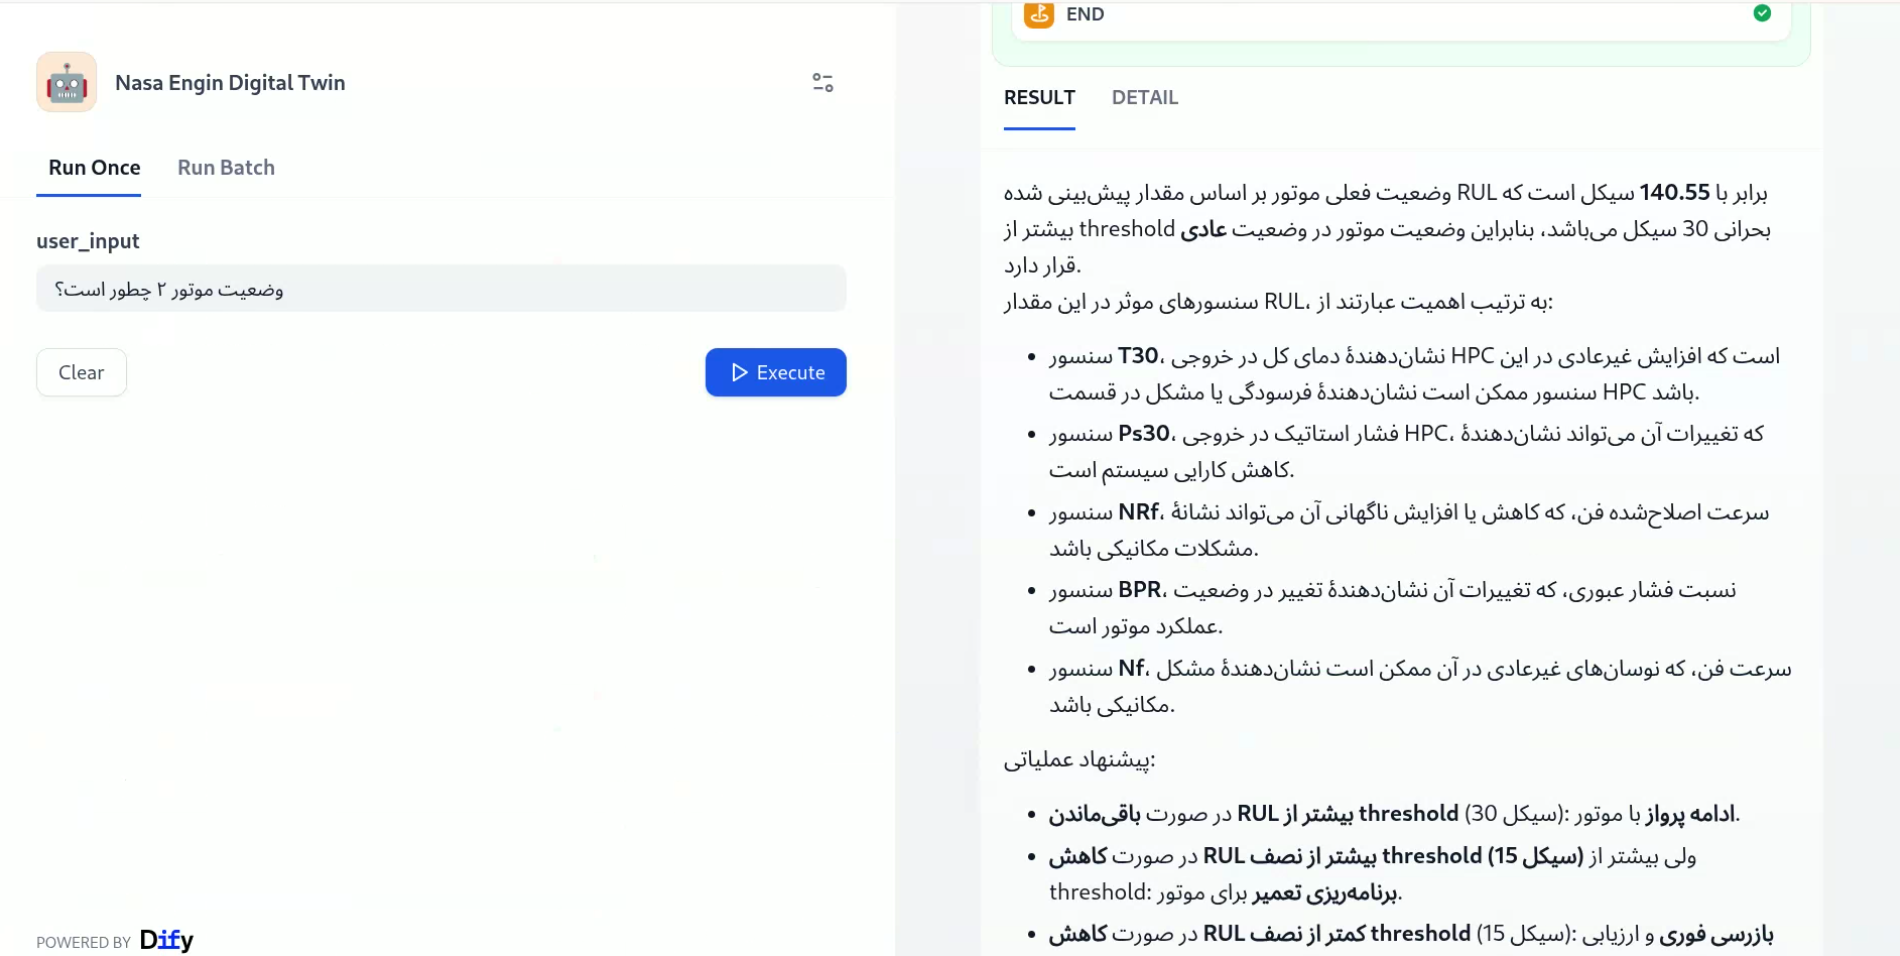
\includegraphics[width=0.95\textwidth]{images/llm_engine2_query.png}
% 	\caption{نمونه پاسخ عامل زبانی برای پرس‌وجوی وضعیت موتور ۲}
% 	\label{fig:llm-engine2-final}
% \end{figure}

% \begin{figure}[H]
% 	\centering
% 	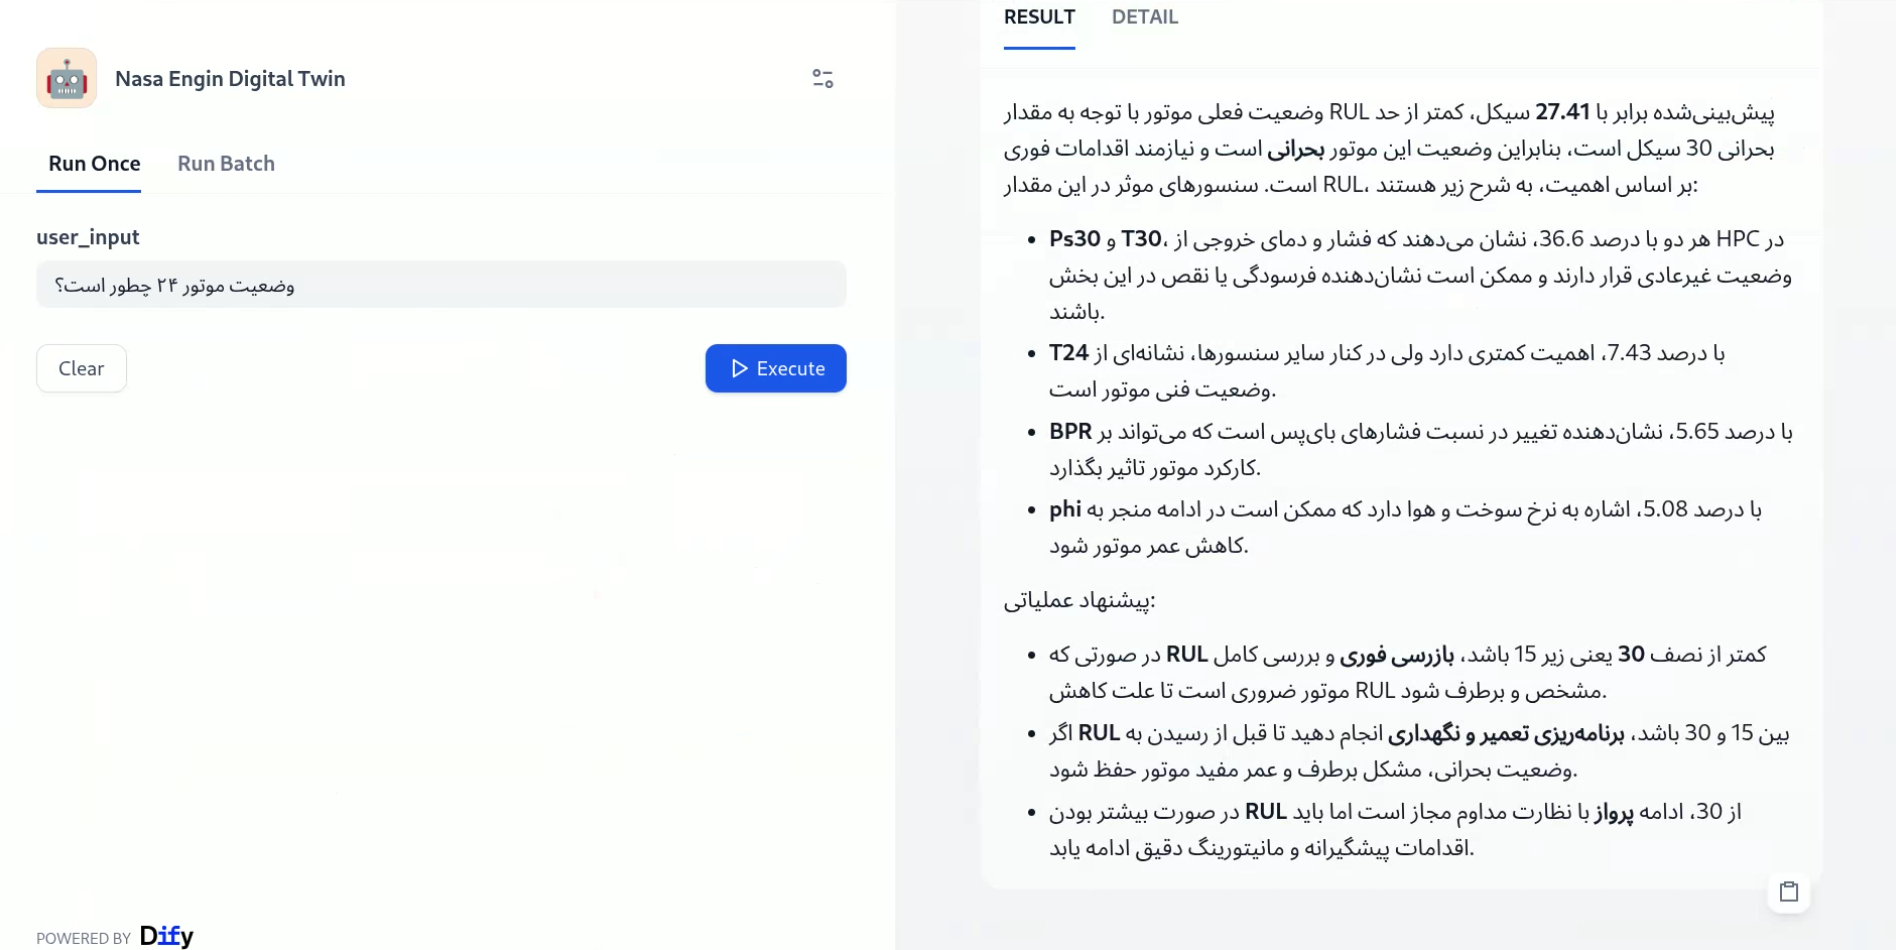
\includegraphics[width=0.95\textwidth]{images/llm_engine24_query.png}
% 	\caption{نمونه پاسخ عامل زبانی برای پرس‌وجوی وضعیت موتور ۲۴}
% 	\label{fig:llm-engine24-final}
% \end{figure}

نکته مهم آن است که عامل زبانی مقدار \gls{RUL} را به صورت مستقل محاسبه نمی‌کند. مقدار عددی از سرویس پیش‌بینی دریافت می‌شود و مدل زبانی بزرگ صرفاً وظیفه تفسیر و ارائه آن را بر عهده دارد. این معماری از نظر قابلیت اعتماد اهمیت دارد، زیرا محاسبه عددی در یک سرویس تخصصی و قابل ارزیابی باقی می‌ماند و مدل زبانی در نقش واسط و هماهنگ‌کننده قرار می‌گیرد.

در فرایند موتور ۲۴ نمایش داد شده در شکل 
\ref{qa:llm-engine-query-24}
، عامل زبانی علاوه بر بیان مقدار \gls{RUL}، مهم‌ترین حسگرهای مؤثر را نیز به کاربر معرفی کرده و برای هر یک تفسیری ارائه می‌دهد. این قابلیت، خروجی یک مدل عددی را به اطلاعاتی تبدیل می‌کند که برای کاربر نهایی قابل استفاده‌تر است.


\subsection{ارزیابی زمان پاسخ}

علاوه بر صحت مسیرهای عملیاتی، زمان پاسخ عامل زبانی نیز اندازه‌گیری شده است. برای ۳۰ درخواست بررسی‌شده، توزیع زمان پاسخ دارای دو ناحیه اصلی است.

\begin{figure}[H]
	\centering
	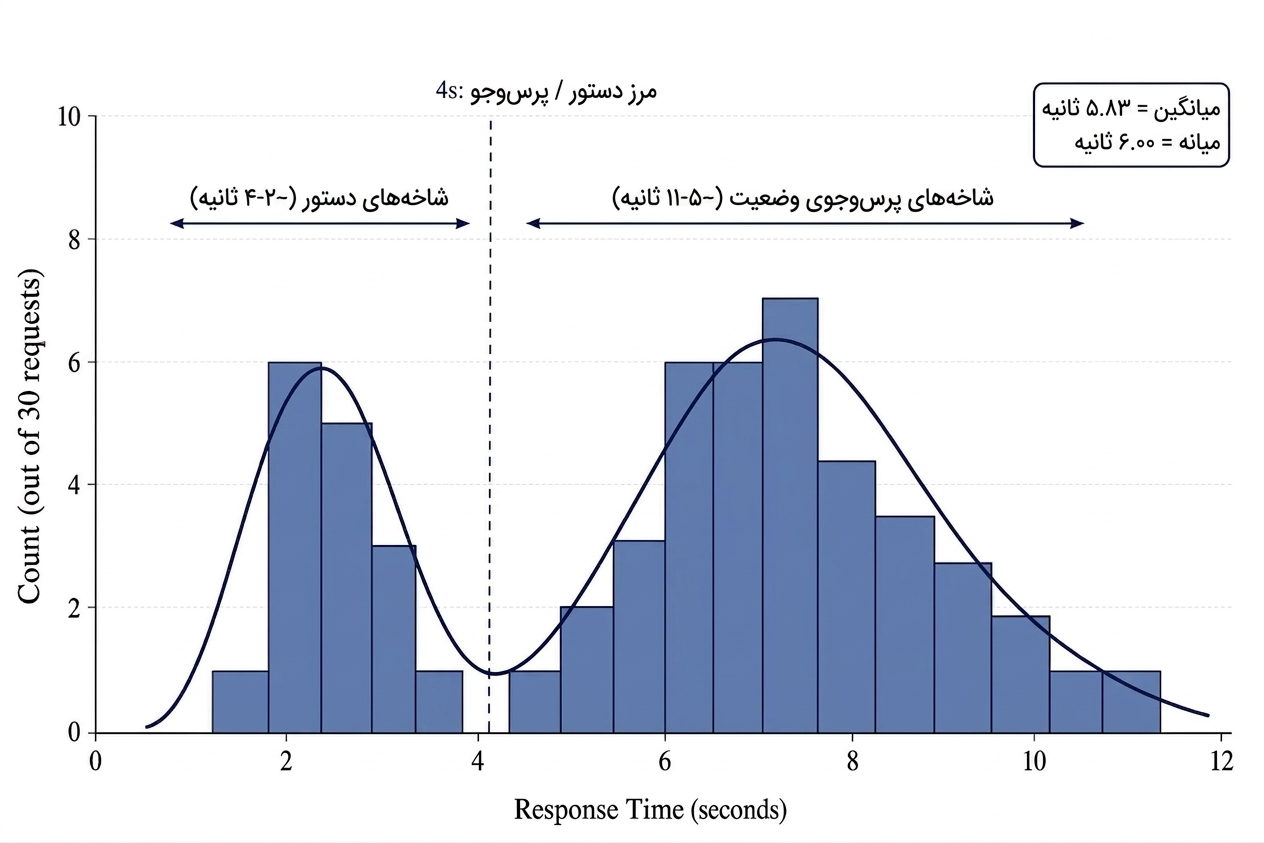
\includegraphics[width=0.90\textwidth]{images/latency_histogram2.png}
	\caption{توزیع زمان پاسخ عامل زبانی برای ۳۰ درخواست}
	\label{fig:latency-hist-final}
\end{figure}

با توجه به نمودار 
\ref{fig:latency-hist-final}،
بخش اول در حدود ۲ تا ۴ ثانیه مربوط به درخواست‌های ساده کنترلی است، درحالی‌که درخواست‌های مربوط به وضعیت موتور به دلیل طی‌کردن چند مرحله، زمان بیشتری نیاز دارند.

\begin{figure}[H]
	\centering
	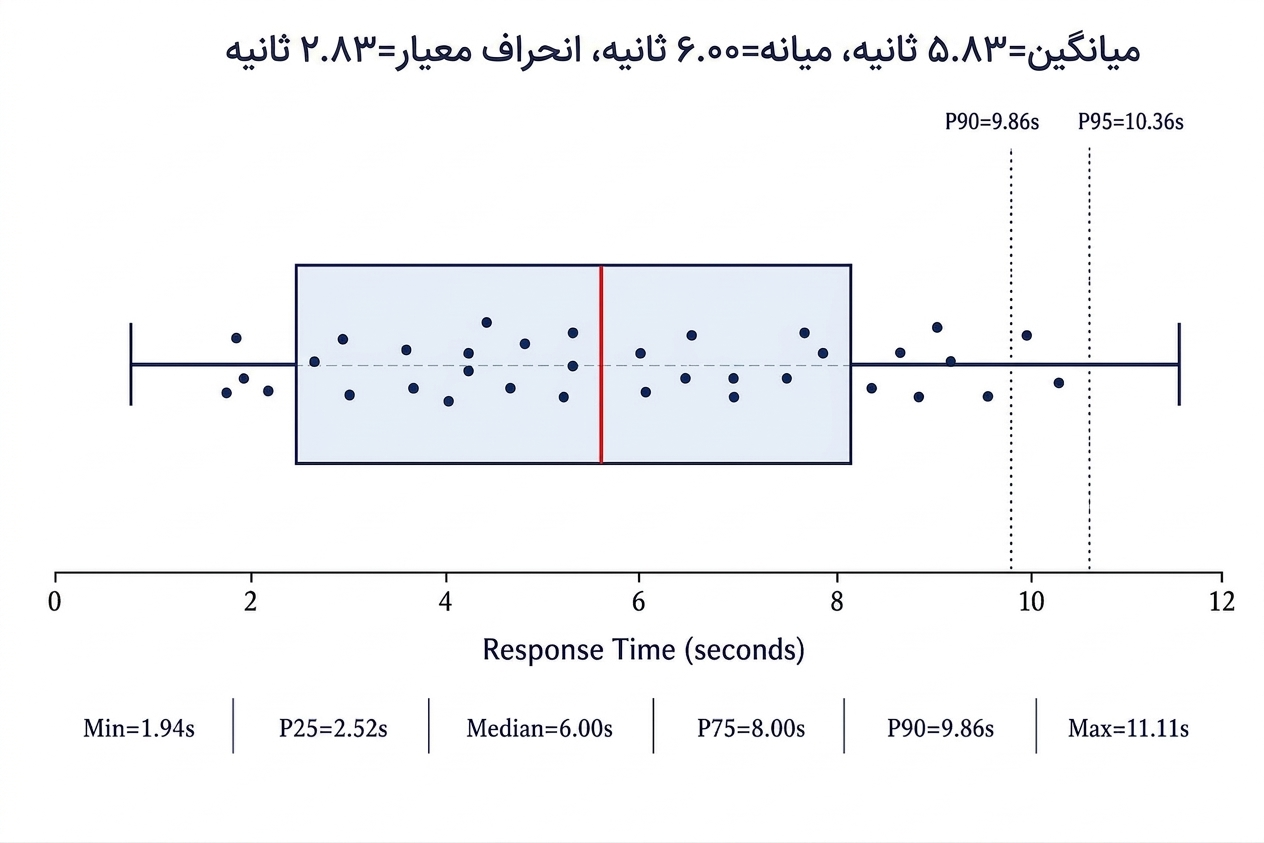
\includegraphics[width=0.90\textwidth]{images/latency_boxplot2.png}
	\caption{نمودار جعبه‌ای زمان پاسخ عامل زبانی}
	\label{fig:latency-box-final}
\end{figure}

در نمودار جعبه‌ای 
\ref{fig:latency-box-final}
نیز مشخص است  که
میانه زمان پاسخ حدود ۶ ثانیه و صدک نودم برابر ۹٫۸۶ ثانیه به دست آمده است. این مقدار برای نمونه آزمایشگاهی حاضر قابل قبول است، اما برای یک سامانه صنعتی بلادرنگ نمی‌توان صرفاً بر همین نتیجه تکیه کرد. کاهش وابستگی به API خارجی، استفاده از مدل‌های سبک‌تر، حافظه نهان، پردازش محلی و روش‌های رویدادمحور می‌توانند زمان پاسخ را کاهش دهند.

\section{ارزیابی پایش و حلقه بسته تصمیم}
\label{sec:closed-loop-evaluation}

مهم‌ترین تفاوت میان یک مدل پیش‌بینی مستقل و معماری پیشنهادی، در امکان تبدیل خروجی پیش‌بینی به یک جریان عملیاتی است. در فصل چهارم، این جریان در سطح پیاده‌سازی نشان داده شد. در این فصل، نتیجه آن از دیدگاه ارزیابی معماری بررسی می‌شود.

در فرایند نخست، کاربر درباره وضعیت یک موتور پرس‌وجو می‌کند. درخواست پس از تشخیص نیت، به عامل پیش‌بینی ارسال می‌شود و نتیجه به عامل زبانی بازمی‌گردد. عامل زبانی نتیجه را به شکل قابل فهم ارائه می‌کند.

در فرایند دوم، کاربر دستور می‌دهد موتورهای در معرض خطر خاموش شوند. در این حالت، مسیر به صورت جریان 
\ref{eq:flow}
طی می‌شود.

\begin{equation}
	\label{eq:flow}
	\text{پیش‌بینی}
	\rightarrow
	\text{تصمیم}
	\rightarrow
	\text{کنترل}
	\rightarrow
	\text{به‌روزرسانی وضعیت}
	\rightarrow
	\text{مشاهده وضعیت}
\end{equation}


این حلقه نشان می‌دهد که دوقلوی دیجیتال در پیاده‌سازی حاضر تنها یک مخزن اطلاعات نیست. تغییر وضعیت ایجادشده توسط فرمان نیز به دوقلو بازمی‌گردد و در نمایش پایش قابل مشاهده می‌شود. چنین ویژگی‌ای با مفهوم دوقلوی دیجیتال به عنوان یک سیستم پویا و متصل به موجودیت متناظر سازگارتر است \cite{tao2018digital,qi2021enabling}.

\begin{figure}[H]
	\centering
	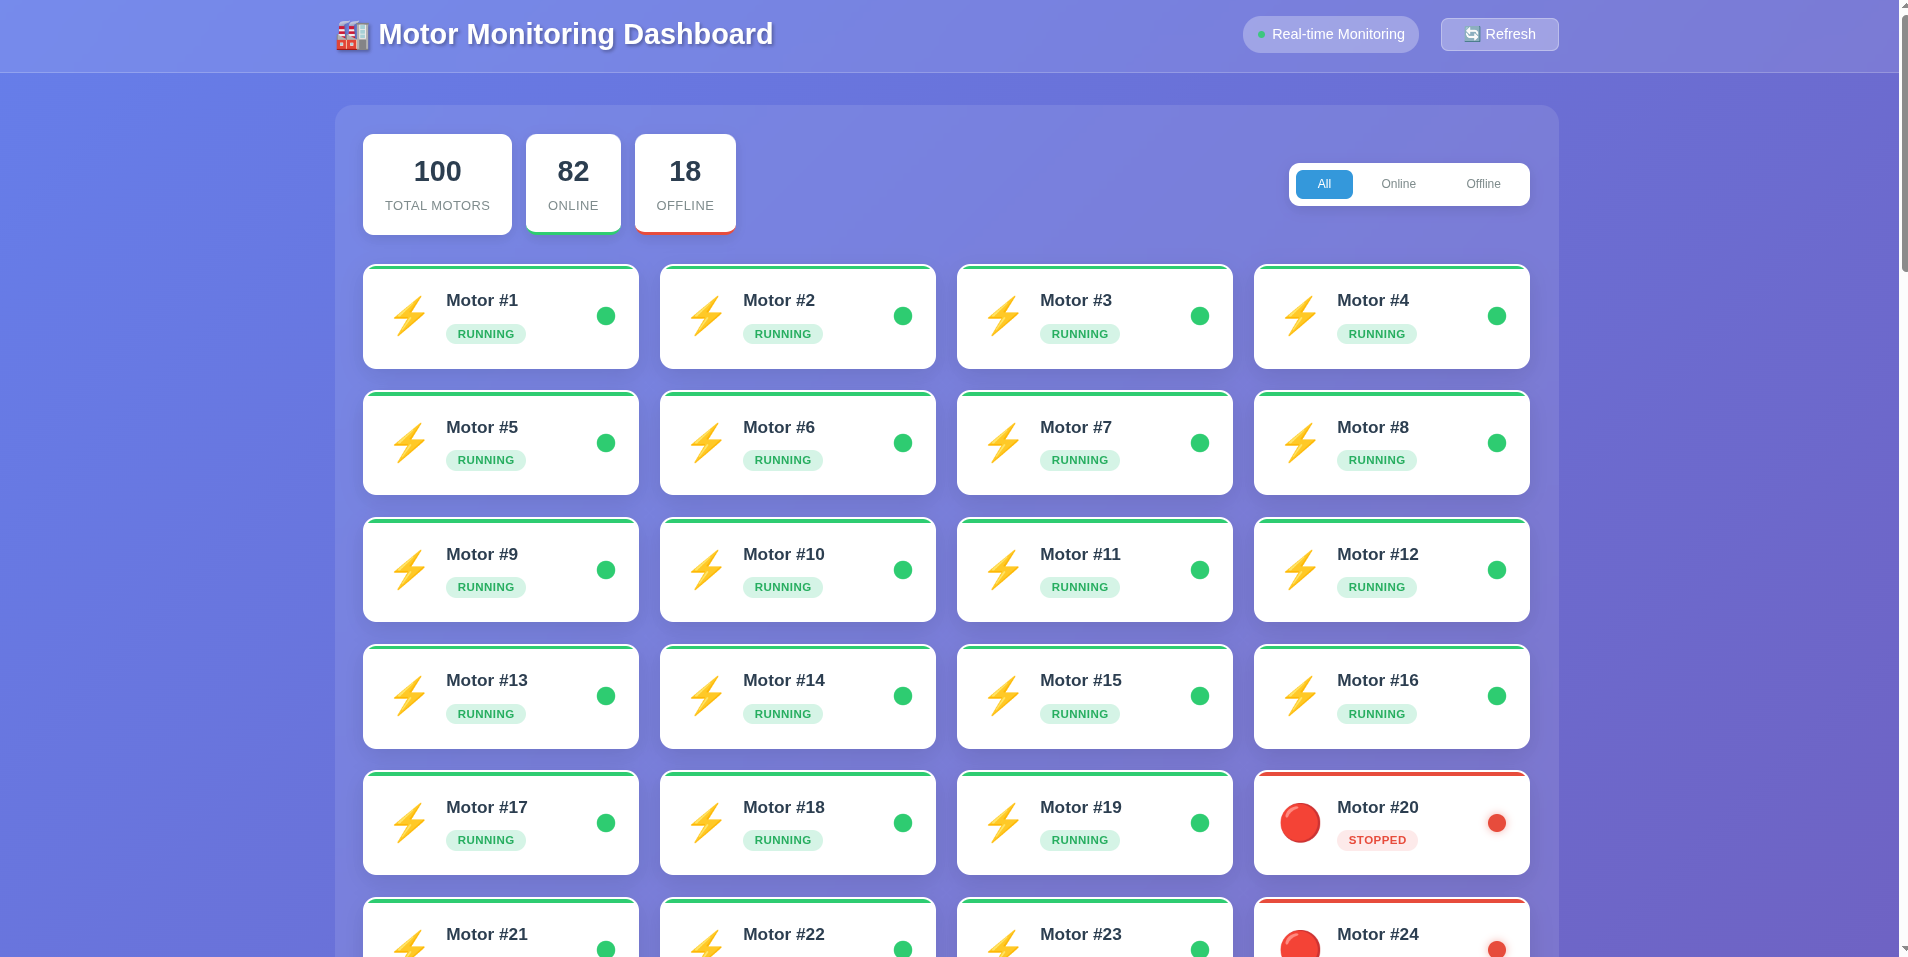
\includegraphics[width=0.90\textwidth]{images/monitor_after_critical_off.png}
	\caption{رابط پایش پس از اجرای فرمان خاموش‌سازی موتورهای در معرض خطر}
	\label{fig:closed-loop-final}
\end{figure}

از منظر معماری، این آزمایش اهمیت بیشتری از یک پاسخ موفق مدل زبانی بزرگ دارد؛ زیرا نشان می‌دهد چند سرویس مستقل توانسته‌اند یک فرایند مشترک را تکمیل کنند. عامل پیش‌بینی بدون عامل دوقلو نمی‌تواند وضعیت عملیاتی را تغییر دهد، عامل زبانی بدون سرویس پیش‌بینی نمی‌تواند درباره \gls{RUL} پاسخ تخصصی ارائه کند و عامل پایش بدون دریافت خروجی پیش‌بینی قادر به تشخیص موتورهای کم‌عمر نیست. بنابراین، ارزش معماری دقیقاً در تعامل این اجزا آشکار می‌شود.




% -----------------------------------------------------------------------
\section{مقایسه با پژوهش‌های مرتبط}
\label{sec:comparison}

هدف از این بخش، مشخص کردن جایگاه پژوهش حاضر نسبت به پژوهش‌هایی است که هر یک بخشی از مسئله مورد نظر این پژوهش را بررسی کرده‌اند. از این رو، چند پژوهش پایه از حوزه‌های دوقلوهای دیجیتال، سیستم‌های چندعاملی، نگهداری پیش‌بینانه و مدل‌های زبانی بزرگ انتخاب شده‌اند و قابلیت‌های آن‌ها در کنار قابلیت‌های چارچوب پیشنهادی مقایسه می‌شود.

موهانراج
 و
بالاجی
در سال ۲۰۲۶ در یک مرور جامع، روند توسعه فناوری
دوقلوهای دیجیتال، معماری‌ها، کاربردها، روش‌های مدل‌سازی و چالش‌های
یکپارچه‌سازی آن با فناوری‌هایی مانند هوش مصنوعی و اینترنت اشیاء را
بررسی کرده‌اند \cite{mohanraj2026digitaltwin}. یکی از نکات مهم این
مطالعه، تأکید بر ضرورت حرکت دوقلوهای دیجیتال از یک نمایش مجازی ساده به
سمت سامانه‌هایی یکپارچه، داده‌محور و هوشمند است. همچنین موضوعاتی مانند
مقیاس‌پذیری، قابلیت همکاری و یکپارچه‌سازی اجزای مختلف به عنوان مسائل
مهم توسعه دوقلوهای دیجیتال آینده مطرح شده‌اند. پژوهش حاضر این دیدگاه
را در سطح پیاده‌سازی دنبال می‌کند. به این صورت که دوقلوی دیجیتال،
عامل پایش، عامل پیش‌بینی و عامل مدل زبانی به صورت اجزای مستقل در یک معماری واحد قرار گرفته‌اند. بنابراین، سهم پژوهش حاضر
در این بخش، تبدیل قابلیت‌های عمومی مطرح‌شده در مطالعه‌ی مروری به یک
نمونه اجرایی قابل آزمایش است.

در حوزه ترکیب سیستم‌های چندعاملی و دوقلوهای دیجیتال،
کولیبالی
و
هملیش
در سال ۲۰۲۶ یک مرور نظام‌مند بر بیش از ۵۴۷ پژوهش انجام داده‌اند
و ضمن ارائه طبقه‌بندی معماری‌های ترکیبی، چالش‌های موجود در کاربرد
دوقلوهای دیجیتال چندعاملی برای نگهداری پیش‌بینانه را بررسی کرده‌اند
\cite{coulibaly2026madtdt}. اهمیت این پژوهش برای پژوهش حاضر
بیش از یک مطالعه مروری معمولی است، زیرا نویسندگان سه مسئله باز را به
عنوان مسیرهای اصلی پژوهش آینده مطرح می‌کنند که یکی از مسئله‌ها، سازمان‌دهی سلسله‌مراتبی دوقلوهای دیجیتال برای کنترل هوشمند که در آن برآورد عمر مفید باقیمانده و هوش مصنوعی توضیح‌پذیر نیز در نظر گرفته شود.

این مسئله مطرح‌شده توسط کولیبالی و هملیش ارتباط مستقیمی با جایگاه
پژوهش حاضر دارد. در آن مقاله بیان می‌شود که هنوز سامانه‌ای که بتواند
دوقلوهای دیجیتال، هماهنگی عامل‌ها، برآورد عمر مفید باقیمانده و
توضیح‌پذیری را در یک راهکار یکپارچه و سلسله‌مراتبی برای کاربردهای
صنعتی ترکیب کند، به طور کامل ارائه نشده است
\cite{coulibaly2026madtdt}. پژوهش حاضر بخشی از این خلأ را در یک
نمونه اجرایی مشخص پوشش می‌دهد. در این پژوهش، عامل پیش‌بینی \gls{RUL} در
کنار عامل دوقلوی دیجیتال و سایر عامل‌های کاربردی قرار گرفته و خروجی
پیش‌بینی نیز مستقیماً در اختیار عامل مدل زبانی قرار می‌گیرد. به این
ترتیب، نتیجه پیش‌بینی تنها یک مقدار عددی نیست، بلکه می‌تواند از طریق زبان طبیعی برای کاربر توضیح داده شود و بر اساس شرایط موتور، پیشنهاد عملی ارائه کند. بنابراین، پژوهش حاضر می‌تواند یک نمونه عملی از این مسئله باز را ارائه دهد و به عنوان یک گام اجرایی در راستای پرسش باز این مقاله در نظر گرفته شود.

از سوی دیگر، پژوهش کولیبالی و هملیش عمدتاً بر طبقه‌بندی معماری‌ها،
فناوری‌ها و چالش‌های موجود تمرکز دارد و هدف آن ارائه یک پیاده‌سازی
موردی برای یک تجهیز مشخص نیست. در پژوهش حاضر، مفاهیم مطرح‌شده به یک معماری عملیاتی تبدیل شده‌اند. به گونه‌ای که هر قابلیت
اصلی در قالب یک عامل مستقل قابل توسعه قرار گرفته است. این ویژگی باعث
می‌شود عامل پیش‌بینی بتواند در آینده با مدل دیگری جایگزین شود، بدون
آنکه الزاماً عامل دوقلو یا عامل زبان طبیعی تغییر کند. از این منظر،
چند عاملی بودن معماری پیشنهادی، پاسخی عملی به نیاز مطرح‌شده در مطالعات
جدید برای ایجاد معماری‌های انعطاف‌پذیر و قابل توسعه است.

در حوزه استفاده از مدل‌های زبانی بزرگ،
 فن و همکاران در سال ۲۰۲۶
چارچوبی برای استفاده از مدل زبانی بزرگ در محیط‌های صنعتی مبتنی بر
دوقلوی دیجیتال ارائه کرده‌اند که در آن مدل‌های زبانی بزرگ در فرآیند تصمیم‌گیری و
یادگیری تقویتی مورد استفاده قرار می‌گیرد \cite{fan2026llmrl}. این
پژوهش نشان می‌دهد که مدل‌های زبانی بزرگ می‌توانند دوقلوی دیجیتال را از یک محیط
صرفاً شبیه‌سازی و تحلیل به محیطی برای تصمیم‌گیری هوشمند تبدیل کنند.
با این حال، تمرکز آن بر هدایت فرآیند یادگیری تقویتی است. در حالی که
در پژوهش حاضر مدل زبانی بزرگ در نقش واسط شناختی و تعاملی میان کاربر و دوقلوی
دیجیتال قرار می‌گیرد. عامل زبان طبیعی می‌تواند وضعیت موتور را
بازیابی کند، درباره مقدار \gls{RUL} پرس‌وجو کند، دلیل وضعیت پیش‌بینی‌شده را
بر اساس اطلاعات موجود توضیح دهد و در صورت تعریف دستورات مجاز، فرمان
عملیاتی را به عامل مربوطه منتقل کند.

این تفاوت با جهت‌گیری پژوهش‌های جدید در زمینه عامل‌های هوشمند نیز
هم‌راستا است.
 حسن
 و 
 نگوین
 در سال ۲۰۲۶ بر ترکیب عامل‌های هوشمند و
دوقلوهای دیجیتال برای ایجاد سامانه‌های تصمیم‌گیری هوشمند تأکید
کرده‌اند \cite{hasan2026agenticdt}. در چنین رویکردهایی، دوقلوی دیجیتال
می‌تواند به عنوان منبع وضعیت سامانه و عامل هوشمند به عنوان لایه
استدلال و تصمیم‌گیری عمل کند. پژوهش حاضر این ایده را به یک فرایند
نگهداری پیش‌بینانه منتقل کرده است. به این صورت که عامل زبانی نه
جایگزین دوقلوی دیجیتال یا مدل پیش‌بینی، بلکه به عنوان یک لایه تعامل
روی آن‌ها قرار می‌گیرد. بنابراین، خروجی عددی مدل یادگیری عمیق به
اطلاعات قابل استفاده برای کاربر تبدیل می‌شود.

در بخش پیش‌بینی، پژوهش‌های مبتنی بر مجموعه داده \gls{CMAPSS} عمدتاً
با هدف کاهش خطای پیش‌بینی \gls{RUL} و توسعه معماری‌های یادگیری عمیق انجام
شده‌اند. در پژوهش حاضر نیز \lr{LSTM} به عنوان مدل پایه پیش‌بینی استفاده
شده است؛ با این تفاوت که هدف پژوهش، ارائه بهترین مدل پیش‌بینی برای
\lr{CMAPSS}
 نیست. 
 \lr{LSTM} 
در اینجا یک مؤلفه قابل تعویض در معماری است که وظیفه
فراهم کردن سرویس تخمین \gls{RUL} را بر عهده دارد. از این رو، امکان جایگزینی
آن با مدل‌های دیگر در آینده وجود دارد، بدون آنکه ساختار کلی دوقلوی
دیجیتال چندعاملی نیازمند بازطراحی اساسی باشد.

تفاوت مهم دیگر در نحوه استفاده از خروجی مدل پیش‌بینی است. در بسیاری
از پژوهش‌های \lr{CMAPSS}، خروجی اصلی مدل یک مقدار \gls{RUL} یا مجموعه‌ای از
معیارهای خطای پیش‌بینی است و ارزیابی عمدتاً در سطح مدل انجام می‌شود.
در پژوهش حاضر، این مقدار بخشی از وضعیت دوقلوی دیجیتال محسوب شده و
می‌تواند در اختیار عامل‌های دیگر قرار گیرد. علاوه بر این، تابع زیان
با توجه به اهمیت عملی خطای بیش‌برآورد \gls{RUL} طراحی شده است تا در شرایط
خطا، پیش‌بینی بیش از حد خوش‌بینانه نسبت به وضعیت واقعی موتور تا حد
امکان کاهش یابد. این انتخاب با هدف استفاده صنعتی از سامانه انجام شده
است، زیرا در نگهداری پیش‌بینانه، پیامدهای یک پیش‌بینی بیش از حد
خوش‌بینانه می‌تواند از یک پیش‌بینی محافظه‌کارانه بسیار پر هزینه‌‌تر باشد.

برآیند این مطالعات نشان می‌دهد که هر یک از پژوهش‌های پایه بخش مهمی
از چارچوب مورد نیاز را پوشش داده‌اند، اما تمرکز آن‌ها متفاوت است.
مقایسه قابلیت‌های اصلی در جدول \ref{tab:comparison-capabilities}
ارائه شده است.

\begin{table}[ht]
	\centering
	\caption{مقایسه قابلیت‌های پژوهش حاضر با پژوهش‌های پایه}
	\label{tab:comparison-capabilities}
	\resizebox{\textwidth}{!}{
		\begin{tabular}{p{4.4cm}ccccc}
			\toprule
			\textbf{قابلیت} &
			\textbf{موهانراج و بالاجی (۲۰۲۶)} &
			\textbf{کولیبالی و هملیش (۲۰۲۶)} &
			\textbf{فن و همکاران (۲۰۲۶)} &
			\textbf{حسن و نگوین (۲۰۲۶)} &
			
			\textbf{پژوهش حاضر} \\
			\midrule
			دوقلوی دیجیتال &
			\checkmark & \checkmark & \checkmark & \checkmark & \textbf{\checkmark} \\
			سیستم چندعاملی &
			-- & \checkmark & محدود & \checkmark & \textbf{\checkmark} \\
			معماری ماژولار و عامل‌های مستقل &
			محدود & \checkmark & محدود & \checkmark & \textbf{\checkmark} \\
			پیش‌بینی RUL &
			محدود & \checkmark & -- & -- & \textbf{\checkmark} \\
			استفاده از LSTM &
			-- & -- & -- & -- & \textbf{\checkmark} \\
			استفاده از CMAPSS &
			-- & -- & -- & -- & \textbf{\checkmark} \\
			کاهش هدفمند بیش‌برآورد RUL &
			-- & مطرح‌شده & -- & -- & \textbf{\checkmark} \\
			پایش وضعیت تجهیز &
			\checkmark & \checkmark & \checkmark & \checkmark & \textbf{\checkmark} \\
			دوقلوی دیجیتال دوطرفه در نمونه اجرایی &
			محدود & مطرح‌شده & محدود & محدود & \textbf{\checkmark} \\
			ادغام LLM با DT &
			-- & -- & \checkmark & \checkmark & \textbf{\checkmark} \\
			تعامل با زبان طبیعی &
			-- & -- & \checkmark & \checkmark & \textbf{\checkmark} \\
			توضیح خروجی پیش‌بینی برای کاربر &
			-- & \textbf{هدف آینده} & محدود & محدود & \textbf{\checkmark} \\
			ارائه پیشنهاد به کاربر &
			-- & \textbf{هدف آینده} & محدود & محدود & \textbf{\checkmark} \\
			نمونه اجرایی CMAPSS + MA-DT + LSTM + LLM &
			-- & -- & -- & -- & \textbf{\checkmark} \\
			\bottomrule
	\end{tabular}}
\end{table}

جدول \ref{tab:comparison-capabilities} نشان می‌دهد که پژوهش حاضر
در یک ویژگی منفرد لزوماً جایگزین پژوهش‌های پیشین نیست، بلکه قابلیت‌هایی
را که پیش‌تر عمدتاً به صورت جداگانه بررسی شده‌اند، در یک معماری واحد
به یکدیگر متصل می‌کند. این موضوع به ویژه در ارتباط با یافته‌های
\lr{Coulibaly}
و
\lr{Hamlich} 
 اهمیت دارد؛ زیرا مسئله‌ای که آن‌ها در سطح مرور
ادبیات به عنوان یک پرسش باز مطرح کرده‌اند، یعنی ترکیب دوقلوی دیجیتال،
هماهنگی عامل‌ها، برآورد \gls{RUL} و توضیح‌پذیری، در پژوهش حاضر در سطح یک
نمونه اجرایی مشخص دنبال شده است.

بنابراین، جایگاه پژوهش حاضر را می‌توان ایجاد یک پل میان چهار مسیر
اصلی پژوهش دانست. دوقلوی دیجیتال برای نمایش و همگام‌سازی وضعیت
موجودیت، سیستم چندعاملی برای تفکیک و مدیریت خدمات، یادگیری عمیق برای
تخمین \gls{RUL} و مدل زبانی بزرگ برای تعامل، توضیح و تصمیم‌یار. مزیت این ترکیب در اجزای مستقل و قابل تعویض آن است؛ به گونه‌ای که مدل پیش‌بینی، روش تعامل کاربر یا حتی نوع موجودیت فیزیکی می‌تواند در آینده تغییر کند، بدون آنکه اصل معماری نیازمند تغییر اساسی باشد.




\section{مزیت‌های معماری پیشنهادی}
\label{sec:architecture-benefits}

مهم‌ترین مزیت پژوهش حاضر را می‌توان در ترکیب چند قابلیت در یک معماری واحد دانست. هر یک از فناوری‌های استفاده‌شده پیش از این به صورت مستقل در پژوهش‌های مختلف بررسی شده‌اند، اما معماری حاضر تلاش می‌کند آن‌ها را در قالب یک زنجیره عملیاتی منسجم کنار یکدیگر قرار دهد.

نخستین مزیت، \textbf{جداسازی مسئولیت‌ها} است. عامل دوقلو، عامل پیش‌بینی، عامل پایش و عامل زبانی وظایف متفاوتی دارند. این جداسازی امکان جایگزینی هر جزء را بدون بازطراحی کل سامانه فراهم می‌کند.

دومین مزیت، \textbf{قابلیت توسعه} است. برای نمونه، می‌توان مدل LSTM را با مدل دیگری جایگزین کرد، بدون آنکه عامل زبانی یا رابط پایش تغییر اساسی کند.

سومین مزیت، \textbf{قابلیت تعامل طبیعی} است. کاربر برای دریافت وضعیت موتور مجبور نیست مستقیماً API یا ساختار داده را بشناسد و می‌تواند درخواست خود را به زبان طبیعی بیان کند.

چهارمین مزیت، \textbf{قابلیت اقدام} است. عامل زبانی صرفاً وضعیت را توضیح نمی‌دهد، بلکه در چارچوب فرمان‌های تعریف‌شده می‌تواند درخواست تغییر وضعیت را به دوقلوی دیجیتال منتقل کند.

پنجمین مزیت، \textbf{توجه به هزینه نامتقارن خطا} است. مدل پیش‌بینی با هدف یک کاربرد نگهداری، طراحی شده است و صرفاً به کمینه‌سازی خطا محدود نیست.

ششمین مزیت، \textbf{قابلیت توضیح خروجی} است. ترکیب وزن‌های توجه، داده حسگرها و عامل زبانی امکان ارائه توضیحی قابل فهم‌تر از یک مقدار عددی خام را فراهم کرده است.

هفتمین مزیت، \textbf{قابلیت انتقال معماری} است. از آنجا که ارتباط میان عامل‌ها از طریق سرویس‌ها و قراردادهای مشخص انجام می‌شود، می‌توان در آینده منبع داده یا مدل پیش‌بینی را تغییر داد.




\section{محدودیت‌های پژوهش}
\label{sec:limitations-final}

با وجود نتایج به‌دست‌آمده، برای جلوگیری از تعمیم بیش از حد یافته‌ها، محدودیت‌های پژوهش باید به‌صورت صریح بیان شوند.

نخستین محدودیت به مجموعه داده مربوط است. آزمایش کمی تنها روی \lr{FD001} انجام شده است. این زیرمجموعه یک شرایط عملیاتی و یک حالت خرابی دارد و بنابراین نمی‌توان نتایج حاصل را مستقیماً به \lr{FD002} تا \lr{FD004} یا شرایط واقعی عملیاتی تعمیم داد.

دومین محدودیت، مصنوعی بودن داده‌ها است. اگرچه \gls{CMAPSS} یکی از مجموعه داده‌های استاندارد و پرکاربرد در پژوهش‌های نگهداری پیش‌بینانه است، داده‌های آن جایگزین داده‌های حسگر واقعی موتور در حال بهره‌برداری نیستند. بنابراین، سامانه حاضر باید به عنوان یک نمونه آزمایشگاهی و اثبات امکان‌پذیری معماری تفسیر شود، نه یک سامانه آماده بهره‌برداری روی موتور واقعی.

سومین محدودیت، شبه‌بی‌درنگ بودن داده‌ها است. داده‌ها از فایل‌های CMAPSS استخراج و با پیشرفت ساعت شبیه‌سازی وارد سامانه شده‌اند. بنابراین، عملکرد واقعی شبکه حسگر، تأخیر ارتباطی، خرابی حسگر و نویز محیط واقعی در این آزمایش ارزیابی نشده است.

چهارمین محدودیت، نگهداری وضعیت در حافظه است. وضعیت ON/OFF موتور در نمونه فعلی پایدار نیست و با راه‌اندازی مجدد کانتینر از بین می‌رود. برای محیط صنعتی باید از پایگاه داده پایدار یا سامانه‌های مدیریت وضعیت توزیع‌شده استفاده شود.

پنجمین محدودیت، وابستگی عامل زبانی به سرویس بیرونی است. زمان پاسخ و هزینه فراخوانی مدل زبانی در مقیاس صنعتی می‌تواند اهمیت زیادی پیدا کند.

ششمین محدودیت، استفاده از آستانه‌های ثابت است. آستانه‌های وضعیت موتور در نسخه فعلی ثابت هستند، درحالی‌که یک سامانه صنعتی می‌تواند به آستانه‌های وابسته به شرایط عملیاتی، نوع موتور و وضعیت تاریخی تجهیز نیاز داشته باشد.

هفتمین محدودیت، نبود ارزیابی رسمی متخصصان حوزه هوافضا برای توضیحات تولیدشده توسط مدل زبانی بزرگ است. پاسخ‌های تولیدشده در این پژوهش از نظر ساختاری و عملکردی بررسی شده‌اند، اما اعتبار فیزیکی همه توضیحات حسگری باید در آینده توسط متخصصان موتور و نگهداری ارزیابی شود.



\section{جمع‌بندی}
\label{sec:chapter5-summary}
در این فصل، عملکرد سامانه پیشنهادی از دو منظر مدل پیش‌بینی و معماری چندعاملی ارزیابی شد تا مشخص شود آیا چارچوب ارائه‌شده توانایی تبدیل یک مدل پیش‌بینی عمر مفید باقیمانده به بخشی از یک سامانه یکپارچه برای پایش، تفسیر و تصمیم‌گیری را دارد یا خیر. ارزیابی کمی مدل پیش‌بینی بر روی زیرمجموعه \lr{FD001} از مجموعه داده \gls{CMAPSS} انجام شد و عملکرد مدل پایه و نسخه نهایی \lr{V2} با استفاده از معیارهای \lr{MAE}، \lr{RMSE}، $R^2$ و نسبت کم‌برآورد مورد مقایسه قرار گرفت. نتایج نشان داد که مدل \lr{V2} با استفاده از سازوکار توجه و تابع زیان \lr{Pinball} با $\tau=0.125$ توانسته است \lr{MAE} را از ۱۷٫۵۶ به ۱۷٫۲۱ کاهش دهد و مقدار $R^2$ را از ۰٫۲۴ به ۰٫۷۱ افزایش دهد. همچنین، نسبت کم‌برآورد از ۰٫۴۷ در مدل پایه به ۰٫۸۷ در مدل نهایی افزایش یافت. این تغییر در نسبت کم‌برآورد به عنوان یک ویژگی طراحی‌شده و مرتبط با هدف ایجاد رفتار محافظه‌کارانه در پیش‌بینی تفسیر شد، نه صرفاً به عنوان یک بهبود عمومی در دقت مدل. در عین حال، نتایج نشان دادند که این انتخاب نباید به معنای تلاش برای بیشینه‌سازی کم‌برآورد تلقی شود، زیرا کم‌برآورد بیش از حد نیز می‌تواند به افزایش بازرسی‌ها و اقدامات نگهداری غیرضروری منجر شود. از این رو، مقدار $\tau=0.125$ در این پژوهش به عنوان یک انتخاب اولیه و محافظه‌کارانه برای قرار دادن مدل در زنجیره تصمیم‌گیری در نظر گرفته شده است.

از منظر معماری، نتایج نشان داد که مدل \lr{LSTM} به عنوان یک مؤلفه تخصصی و قابل تعویض، توانسته است سرویس پیش‌بینی مورد نیاز معماری را فراهم کند، بدون آنکه مدل پیش‌بینی به هسته اصلی معماری وابسته باشد. این موضوع با هدف کلی پژوهش سازگار است، زیرا مسئله اصلی پژوهش رقابت میان مدل‌های مختلف یادگیری عمیق برای دستیابی به کمترین خطای ممکن روی \gls{CMAPSS} نبوده است؛ بلکه هدف، قرار دادن یک مدل پیش‌بینی قابل قبول درون یک معماری چندعاملی بوده است. بنابراین، نتایج مدل باید در ارتباط با نقش آن در کل سامانه تفسیر شوند و نه به عنوان ادعایی درباره برتری عمومی \lr{LSTM} یا مدل \lr{V2} نسبت به تمامی روش‌های موجود.

در ادامه، عامل تعامل زبانی از نظر قابلیت اجرای فرایندهای تعریف‌شده، تفسیر خروجی پیش‌بینی و زمان پاسخ مورد بررسی قرار گرفت. در ۳۰ درخواست آزمایش‌شده، نرخ موفقیت فرایندهای تعریف‌شده ۱۰۰ درصد به دست آمد. این ارزیابی نشان داد که عامل زبانی می‌تواند مقدار \gls{RUL} دریافت‌شده از سرویس پیش‌بینی را به اطلاعات قابل فهم برای کاربر تبدیل کند. همچنین می‌تواند وضعیت موتور را بر اساس آستانه‌های تعریف‌شده تفسیر نماید و در چارچوب فرمان‌های مجاز، درخواست‌های کنترلی را به عامل دوقلوی دیجیتال منتقل کند.علاوه‌ بر این اندازه‌گیری زمان پاسخ نشان داد که میانه زمان پاسخ حدود ۶ ثانیه و صدک نودم برابر با ۹٫۸۶ ثانیه بوده است. این زمان برای نمونه آزمایشگاهی حاضر قابل قبول ارزیابی شد، اما به دلیل وابستگی به سرویس بیرونی و تفاوت میان محیط آزمایشگاهی و محیط صنعتی، نمی‌توان آن را به عنوان تضمین عملکرد بلادرنگ در کاربردهای صنعتی در نظر گرفت.

مهم‌ترین یافته معماری در ارزیابی، حلقه بسته تصمیم است. در این فرایند، خروجی پیش‌بینی به تصمیم‌گیری منتقل شده، تصمیم به فرمان کنترلی تبدیل گردیده، وضعیت دوقلوی دیجیتال به‌روزرسانی شده و نتیجه تغییر وضعیت در لایه پایش قابل مشاهده بوده است. در نتیجه، دوقلوی دیجیتال در نمونه پیاده‌سازی‌شده صرفاً به عنوان یک مخزن اطلاعاتی مورد استفاده قرار نگرفته، بلکه در یک چرخه عملیاتی میان داده، پیش‌بینی، تصمیم، کنترل و بازخورد قرار گرفته است. این ویژگی نشان می‌دهد که ارزش معماری پیشنهادی تنها در عملکرد مستقل هر عامل نیست، بلکه در نحوه همکاری عامل‌های تخصصی برای تکمیل یک فرایند سرتاسری نمایان می‌شود.

مقایسه با پژوهش‌های مرتبط نیز نشان داد که پژوهش حاضر در یک قابلیت منفرد لزوماً جایگزین مطالعات پیشین نیست، بلکه تلاش می‌کند چند مسیر پژوهشی شامل دوقلوهای دیجیتال، سیستم‌های چندعاملی، پیش‌بینی \gls{RUL}، پایش و مدل‌های زبان بزرگ را در قالب یک نمونه اجرایی واحد به یکدیگر متصل کند. جداسازی مسئولیت‌ها میان عامل دوقلوی دیجیتال، عامل پیش‌بینی، عامل پایش و عامل زبان طبیعی، امکان توسعه و جایگزینی مستقل اجزای سامانه را فراهم می‌کند و در عین حال، استفاده از مدل زبانی را از محاسبه مستقیم مقدار \gls{RUL} جدا نگه می‌دارد. بر این اساس، مهم‌ترین نتیجه فصل حاضر آن است که معماری پیشنهادی توانسته است یک مدل پیش‌بینی را از یک مؤلفه مستقل محاسباتی به بخشی از یک زنجیره عملیاتی شامل پیش‌بینی، تفسیر، تصمیم، کنترل و بازخورد تبدیل کند.

در نهایت، محدودیت‌های ارزیابی نیز باید در تفسیر این نتایج مورد توجه قرار گیرند. آزمایش کمی مدل تنها بر روی زیرمجموعه \lr{FD001} مجموعه داده \gls{CMAPSS} انجام شده و جریان داده به صورت شبه‌بی‌درنگ شبیه‌سازی شده است. همچنین وضعیت عملیاتی موتور در نمونه فعلی در یک زیرساخت پایدار ذخیره نمی‌شود و عامل زبان طبیعی به یک سرویس بیرونی وابسته است. بنابراین، نتایج این فصل را باید در چارچوب یک نمونه آزمایشگاهی و اثبات امکان‌پذیری معماری تفسیر کرد. با وجود این محدودیت‌ها، مجموعه آزمایش‌های انجام‌شده نشان می‌دهد که اجزای اصلی معماری پیشنهادی توانسته‌اند در کنار یکدیگر یک جریان عملیاتی منسجم ایجاد کنند و مبنای مناسبی برای جمع‌بندی نهایی پژوهش و بررسی دستاوردها و مسیرهای توسعه آینده فراهم آورند.



% \section{پیشنهادهایی برای کارهای آینده}
% \label{sec:future-work-final}

% مسیرهای آینده پژوهش را می‌توان در چهار دسته اصلی تقسیم کرد.

% در دسته نخست، باید دامنه داده گسترش یابد. آزمایش روی \lr{FD002} تا \lr{FD004} می‌تواند میزان مقاومت مدل و معماری را در برابر شرایط عملیاتی مختلف مشخص کند. همچنین استفاده از داده‌های واقعی حسگرهای موتور می‌تواند فاصله میان نمونه آزمایشگاهی و کاربرد صنعتی را کاهش دهد.

% در دسته دوم، مدل پیش‌بینی می‌تواند از یک مدل نقطه‌ای به سمت مدل‌های احتمالاتی حرکت کند. ترکیب \lr{LSTM} با سایر مدل‌های احتمالاتی و استفاده از مدل‌های دقیق‌تر با خطای کم‌تر می‌تواند در دقت خروجی مدل کمک کند و در نتیجه خروجی زبان طبیعی را نیز واضح‌تر کند.

% در دسته سوم، عامل زبانی می‌تواند با حافظه بلندمدت، پایگاه دانش فنی و دانش‌نگار حوزه هوافضا ترکیب شود. در این صورت، پاسخ عامل تنها بر اساس مقدار فعلی \gls{RUL} نخواهد بود، بلکه تاریخچه موتور، تعمیرات قبلی، شرایط عملیاتی و سوابق خرابی را نیز در نظر خواهد گرفت.

% در دسته چهارم، معماری می‌تواند به حوزه‌های دیگر منتقل شود. برای مثال، در یک کارخانه تولیدی، عامل دوقلو می‌تواند نماینده یک دستگاه \lr{CNC} باشد؛ عامل پیش‌بینی وضعیت خرابی دستگاه را تخمین بزند؛ عامل پایش وضعیت خط تولید را بررسی کند و عامل زبانی امکان پرس‌وجو و اجرای فرمان را فراهم آورد. به همین ترتیب، معماری می‌تواند برای سایر صنایع مورد نیاز نیز توسعه یابد.

% برای نزدیک شدن به استقرار صنعتی نیز پیشنهاد می‌شود ارتباط سرویس‌ها از مدل نظرسنجی دوره‌ای به سازوکارهای رویدادمحور منتقل شود و وضعیت دوقلو در یک زیرساخت پایدار ذخیره گردد. همچنین لازم است سیاست‌های کنترل دسترسی، ثبت رویداد، تأیید انسانی فرمان‌های حساس و سازوکارهای ایمنی در لایه عامل زبانی اضافه شوند.




% \section{جمع‌بندی نهایی}
% \label{sec:final-summary}

% هدف اصلی این پژوهش طراحی و پیاده‌سازی یک چارچوب دوقلوهای دیجیتال چندعاملی برای پایش و پیش‌بینی عمر مفید موتورهای توربوفن و بررسی امکان تعامل طبیعی با این دوقلوها بود. در این راستا، یک معماری چندلایه طراحی و سپس با استفاده از مجموعه داده \gls{CMAPSS} در قالب یک نمونه آزمایشگاهی پیاده‌سازی شد.

% نتایج نشان داد که مدل LSTM مورد استفاده می‌تواند به عنوان یک مؤلفه پیش‌بینی قابل استفاده در معماری عمل کند. مدل نهایی با استفاده از سازوکار توجه و \gls{PinballLoss} توانست \lr{MAE} برابر ۱۷٫۲۱ و $R^2$ برابر ۰٫۷۱ را روی مجموعه آزمون به دست آورد. همچنین نسبت کم‌برآورد از ۴۷ درصد در مدل پایه به ۸۷ درصد افزایش یافت. اهمیت نتیجه دوم در این است که مدل به صورت هدفمند به سمت پیش‌بینی محافظه‌کارانه حرکت کرده است؛ رویکردی که با ماهیت ایمنی‌محور نگهداری موتورها سازگارتر است. بااین‌حال، این نتایج به معنای ارائه بهترین مدل برای CMAPSS نیست و مدل پیش‌بینی در این پژوهش صرفاً به عنوان یک مؤلفه تخصصی و قابل جایگزینی در معماری در نظر گرفته شده است.

% در سطح سامانه‌ای، عامل زبانی توانست اطلاعات عددی تولیدشده توسط عامل پیش‌بینی را به زبان طبیعی تفسیر کند، وضعیت موتور را توضیح دهد و در فرایند‌های تعریف‌شده، فرمان‌های کنترلی را به دوقلوی دیجیتال ارسال کند. بررسی ۳۰ درخواست، نرخ موفقیت ۱۰۰ درصدی را در فرایند‌های تعریف‌شده نشان داد. همچنین حلقه بسته میان پیش‌بینی، تصمیم، کنترل و بازخورد در فرایند‌های عملیاتی اجرا شد.

% از دیدگاه معماری، مهم‌ترین دستاورد پژوهش در کنار هم قرار دادن قابلیت‌هایی است که معمولاً به صورت جداگانه بررسی می‌شوند: دوقلوی دیجیتال، سیستم چندعاملی، پیش‌بینی \gls{RUL}، پایش شبه‌بی‌درنگ و تعامل مبتنی بر مدل‌های بزرگ زبانی. این ترکیب امکان تبدیل یک مدل پیش‌بینی منفرد به یک سامانه تصمیم‌یار تعاملی را فراهم می‌کند. در چنین ساختاری، مدل یادگیری عمیق صرفاً تولیدکننده یک عدد نیست، بلکه خروجی آن وارد زنجیره‌ای می‌شود که می‌تواند به تشخیص وضعیت، ارائه توضیح، تصمیم‌گیری و در نهایت اقدام منجر شود.

% از منظر کاربرد صنعتی، این پژوهش یک نمونه اثبات امکان‌پذیری ارائه می‌کند و نه یک محصول آماده بهره‌برداری. برای رسیدن به سطح صنعتی، اتصال به داده‌های واقعی حسگر، پایگاه داده پایدار، مدیریت عدم‌قطعیت، اعتبارسنجی متخصصان، کنترل دسترسی و سازوکار تأیید انسانی فرمان‌های حساس ضروری است. با وجود این محدودیت‌ها، ساختار معماری به گونه‌ای طراحی شده است که این اجزا بتوانند در مراحل بعدی بدون تغییر بنیادی در منطق کلی سامانه اضافه شوند.

% در نهایت، می‌توان نتیجه گرفت که ارزش اصلی چارچوب پیشنهادی در \textbf{ترکیب پیش‌بینی، دوقلوی دیجیتال، عامل‌های تخصصی و تعامل زبانی در یک حلقه عملیاتی واحد} است. این ویژگی، معماری را از یک سامانه صرفاً پیش‌بینی‌کننده به سمت یک چارچوب دوقلوی دیجیتال چندعاملی قابل توسعه هدایت می‌کند؛ چارچوبی که می‌تواند در آینده با جایگزینی منبع داده، مدل پیش‌بینی و دانش حوزه، برای سایر تجهیزات و صنایع نیز مورد استفاده قرار گیرد.




%*****************************************************************
% chap6.tex
%*****************************************************************

\chapter{نتیجه‌گیری و پیشنهادها}
\label{chap:conclusion}

\section{مقدمه}
\label{sec}
در فصل‌های پیشین، ابتدا مسئله پژوهش و ضرورت استفاده از دوقلوهای دیجیتال و عامل‌های هوشمند در پایش و نگهداری پیش‌بینانه بررسی شد و سپس مبانی نظری و مطالعات مرتبط با دوقلوهای دیجیتال، سیستم‌های چندعاملی، مدل زبانی بزرگ و پیش‌بینی عمر مفید باقیمانده مورد بررسی قرار گرفت. در ادامه، معماری پیشنهادی دوقلوی دیجیتال چندعاملی طراحی و اجزای آن شامل عامل دوقلوی دیجیتال، عامل پیش‌بینی، عامل تعامل زبانی، عامل پایش و عامل \gls{Dashboard} تعریف و پیاده‌سازی شد. در فصل پنجم نیز عملکرد مدل پیش‌بینی و قابلیت‌های معماری چندعاملی از دید پیش‌بینی، تعامل، پایش و اجرای حلقه بسته تصمیم ارزیابی گردید. فصل حاضر به جمع‌بندی پژوهش و ارائه نتیجه‌گیری نهایی اختصاص دارد و در ادامه، مسیرهای پیشنهادی برای توسعه و تکمیل پژوهش در آینده ارائه می‌شوند. هدف از این فصل، قرار دادن یافته‌های فصل‌های پیشین در یک چارچوب واحد و تبیین میزان تحقق هدف پژوهش بر اساس نتایج به‌دست‌آمده است.

\section{جمع‌بندی پژوهش}
\label{sec:research-summary}
پژوهش حاضر با تمرکز بر مسئله پایش و پیش‌بینی وضعیت موتورهای توربوفن، با هدف بررسی امکان طراحی و پیاده‌سازی یک چارچوب دوقلوی دیجیتال چندعاملی شکل گرفت. مسئله اصلی از این نیاز آغاز شد که یک سامانه نگهداری پیش‌بینانه صرفاً به تولید یک مقدار عددی برای عمر مفید باقیمانده محدود نباشد، بلکه بتواند وضعیت موجودیت را به صورت یکپارچه دریافت و نمایش دهد، خروجی مدل پیش‌بینی را در اختیار اجزای دیگر قرار دهد، اطلاعات حاصل را برای کاربر قابل فهم کند و در چارچوب سیاست‌های تعریف‌شده، امکان انجام اقدامات عملیاتی را نیز فراهم آورد. بر این اساس، پژوهش به جای تمرکز صرف بر توسعه یک مدل یادگیری عمیق مستقل، بر طراحی معماری‌ای متمرکز شد که در آن مدل پیش‌بینی، دوقلوی دیجیتال و عامل‌های کاربردی از جمله زبان طبیعی، بتوانند در قالب یک سامانه واحد با یکدیگر تعامل داشته باشند.

در گام نخست، مبانی نظری مرتبط با دوقلوهای دیجیتال، سیستم‌های چندعاملی، دوقلوهای دیجیتال چندعاملی، مدل‌های زبان بزرگ و نگهداری پیش‌بینانه بررسی شد. مرور مطالعات مرتبط نشان داد که این حوزه‌ها هر یک بخش مهمی از مسئله را پوشش داده‌اند، اما ترکیب آن‌ها در قالب یک معماری اجرایی و یکپارچه همچنان دارای ظرفیت پژوهشی است. بر اساس این بررسی، معماری پیشنهادی با رویکردی ماژولار طراحی شد تا مسئولیت‌های اصلی میان عامل‌های تخصصی توزیع شوند. در این معماری، عامل دوقلوی دیجیتال مسئول نگهداری و ارائه وضعیت موجودیت، عامل پیش‌بینی مسئول تخمین \gls{RUL}، عامل پایش مسئول مشاهده و پیگیری وضعیت، و عامل تعامل زبانی مسئول برقراری ارتباط طبیعی با کاربر و هماهنگی برخی فرایندهای عملیاتی است.
در گام بعد، معماری طراحی‌شده در قالب یک نمونه آزمایشگاهی پیاده‌سازی شد. برای ارزیابی بخش پیش‌بینی، از مجموعه داده \gls{CMAPSS} و به طور مشخص زیرمجموعه \lr{FD001} استفاده شد. مدل \lr{LSTM} در این ساختار به عنوان یک مؤلفه تخصصی و قابل تعویض در نظر گرفته شد و نسخه نهایی آن با استفاده از سازوکار توجه و تابع زیان \lr{Pinball} با هدف ایجاد رفتار محافظه‌کارانه‌تر در برابر بیش‌برآورد \gls{RUL} آموزش داده شد. نتایج ارزیابی نشان داد که این مدل می‌تواند عملکرد مورد نیاز برای ایفای نقش سرویس پیش‌بینی در معماری را فراهم کند. در عین حال، جایگاه مدل در چارچوب پژوهش به گونه‌ای تعریف شد که جایگزینی آن با مدل‌های پیش‌بینی دیگر در آینده، بدون نیاز به بازطراحی اساسی سایر اجزای معماری امکان‌پذیر باشد.

در سطح سامانه، عامل زبانی طبیعی به عنوان واسط میان کاربر و عامل‌های تخصصی قرار می‌گیرد. در این ساختار، محاسبه مقدار \gls{RUL} به مدل زبانی واگذار نشده و مقدار پیش‌بینی‌شده از سرویس تخصصی دریافت می‌گردد. عامل زبانی سپس این مقدار و سایر اطلاعات موجود را برای کاربر تفسیر کرده و در مسیرهای عملیاتی تعریف‌شده، درخواست‌های مناسب را به عامل‌های مربوطه منتقل می‌کند. این جداسازی مسئولیت‌ها سبب شد که محاسبه عددی، تفسیر زبانی و کنترل عملیاتی در عامل‌ها مشخص و قابل ارزیابی باقی بمانند.

در نهایت، اجرای فرایندهای سرتاسری نشان داد که اجزای سامانه می‌توانند در یک زنجیره مشترک با یکدیگر همکاری کنند. در این زنجیره، داده وارد سامانه شده، وضعیت دوقلوی دیجیتال شکل گرفته، مدل پیش‌بینی عمر مفید را تخمین زده، عامل پایش وضعیت را ارزیابی کرده و عامل زبان طبیعی امکان تعامل کاربر با این اطلاعات و انجام فرمان‌های مجاز را فراهم کرده است. همچنین در فرایند حلقه بسته، تغییر ایجادشده در وضعیت عملیاتی دوباره به دوقلوی دیجیتال منتقل شده و در لایه پایش قابل مشاهده است. بنابراین، پژوهش حاضر نشان می‌دهد که می‌توان یک مدل پیش‌بینی و مجموعه‌ای از خدمات مستقل را در قالب یک معماری چندعاملی به یک جریان عملیاتی منسجم تبدیل کرد.

با توجه به مجموعه نتایج، می‌توان گفت مسئله پژوهش از یک دیدگاه صرفاً مدل‌محور به یک دیدگاه سامانه‌محور توسعه یافته است. در این رویکرد، کیفیت سامانه تنها به دقت مدل پیش‌بینی وابسته نیست، بلکه به توانایی اجزای مختلف در همکاری، انتقال اطلاعات، تفسیر نتایج و تبدیل خروجی تحلیلی به اقدام نیز وابسته است. از این رو، معماری پیشنهادی تلاشی برای ایجاد ارتباط میان مدل پیش‌بینی، دوقلوی دیجیتال و لایه تعامل هوشمند است و نمونه پیاده‌سازی‌شده امکان بررسی این ارتباط را در یک فرایند مشخص فراهم کرده است.



% \section{دستاوردها و نوآوری‌های پژوهش}
% \label{sec:contributions}
% مهم‌ترین دستاورد پژوهش حاضر، ارائه و پیاده‌سازی یک معماری دوقلوی دیجیتال چندعاملی است که در آن قابلیت‌های دوقلوی دیجیتال، پیش‌بینی عمر مفید باقیمانده، پایش وضعیت، تعامل زبانی و کنترل عملیاتی در قالب مجموعه‌ای از عامل‌های تخصصی به یکدیگر متصل شده‌اند. این معماری تلاش می‌کند فاصله میان یک مدل پیش‌بینی مستقل و یک سامانه تصمیم‌یار تعاملی را کاهش دهد. در ساختار پیشنهادی، هر عامل مسئولیت مشخصی دارد و ارتباط میان عامل‌ها از طریق رابط‌ها و قراردادهای تعریف‌شده انجام می‌شود. در نتیجه، معماری از یک ساختار یکپارچه و وابسته به یک مدل خاص فاصله گرفته و به سمت ساختاری ماژولار و قابل توسعه حرکت می‌کند.
% یکی از دستاوردهای اصلی پژوهش، تفکیک مسئولیت میان مدل پیش‌بینی و سایر اجزای سامانه است. مدل \lr{LSTM} در این پژوهش به عنوان هسته غیرقابل تغییر سامانه در نظر گرفته نشده، بلکه به عنوان یک مؤلفه تخصصی برای تخمین \gls{RUL} در عامل پیش‌بینی قرار گرفته است. این نحوه سازمان‌دهی باعث می‌شود مدل پیش‌بینی بتواند در آینده با مدل‌های دیگری مانند مدل‌های مبتنی بر \gls{Transformer} یا روش‌های احتمالاتی جایگزین شود، بدون آنکه منطق اصلی عامل دوقلوی دیجیتال، عامل پایش یا عامل تعامل زبانی نیازمند بازطراحی اساسی باشد. از این منظر، سهم پژوهش تنها انتخاب یک مدل یادگیری عمیق نیست، بلکه نحوه قرار دادن این مدل در یک معماری قابل توسعه است.
% دستاورد دیگر، وارد کردن ملاحظه هزینه نامتقارن خطا به زنجیره پیش‌بینی و تصمیم است. در این پژوهش، استفاده از تابع زیان \lr{Pinball} با $\tau=0.125$ با هدف ایجاد گرایش کنترل‌شده به سمت کم‌برآورد \gls{RUL} انجام شد تا احتمال پیش‌بینی بیش از حد خوش‌بینانه کاهش یابد. نتایج آزمایش نشان داد که نسبت کم‌برآورد مدل نهایی نسبت به مدل پایه افزایش یافته است. اهمیت این رویکرد در آن است که عملکرد مدل تنها بر اساس خطای عددی عمومی ارزیابی نشده و نیاز تصمیم‌گیری نگهداری نیز در طراحی آن مورد توجه قرار گرفته است. در عین حال، پژوهش نشان می‌دهد که کم‌برآورد بیش از حد نیز مطلوب نیست و انتخاب پارامتر تابع زیان باید متناسب با هزینه، ریسک و ویژگی‌های تجهیز انجام شود.
% از دیگر دستاوردهای پژوهش، استفاده از مدل زبان بزرگ در نقش یک لایه تعامل و هماهنگی، به جای استفاده از آن به عنوان جایگزین مدل تخصصی پیش‌بینی است. در معماری پیشنهادی، عامل زبانی مقدار \gls{RUL} را به صورت مستقل محاسبه نمی‌کند، بلکه اطلاعات حاصل از سرویس‌های تخصصی را دریافت و به زبان طبیعی برای کاربر تفسیر می‌کند. این تفکیک باعث می‌شود استنتاج عددی و تعامل زبانی از یکدیگر مستقل باقی بمانند و در عین حال، کاربر بتواند بدون تعامل مستقیم با رابط‌های فنی، درباره وضعیت تجهیز پرس‌وجو کند و در چارچوب فرمان‌های تعریف‌شده درخواست عملیاتی ارائه دهد.
% همچنین، پیاده‌سازی حلقه بسته پیش‌بینی، تصمیم، کنترل و بازخورد را می‌توان یکی دیگر از دستاوردهای معماری دانست. در نمونه اجرایی، خروجی پیش‌بینی صرفاً در قالب یک گزارش نمایش داده نشده، بلکه می‌تواند در مسیر تصمیم‌گیری قرار گیرد و نتیجه تصمیم پس از اعمال فرمان به وضعیت دوقلوی دیجیتال بازگردد. در نتیجه، دوقلوی دیجیتال، عامل پیش‌بینی، عامل زبان و عامل پایش در یک فرایند سرتاسری به یکدیگر متصل می‌شوند. این ویژگی، معماری را از یک سامانه صرفاً تحلیلی به سمت یک چارچوب تصمیم‌یار و عملیاتی هدایت می‌کند.
% دستاورد دیگر، ارائه یک نمونه اجرایی برای بررسی هم‌زمان چند قابلیت در یک سناریوی مشخص است. استفاده از \gls{CMAPSS} امکان ارزیابی مدل پیش‌بینی را فراهم کرده و سرویس‌های پیاده‌سازی‌شده نیز امکان بررسی تعامل میان پیش‌بینی، دوقلوی دیجیتال، پایش و عامل زبان را فراهم ساخته‌اند. از این رو، پژوهش حاضر علاوه بر تعریف معماری در سطح مفهومی، امکان بررسی رفتار آن را در سطح پیاده‌سازی و اجرای فرایندهای سرتاسری نیز فراهم کرده است.
% در مجموع، نوآوری اصلی پژوهش را می‌توان در سطح معماری و یکپارچه‌سازی قابلیت‌ها تعریف کرد. ارزش چارچوب پیشنهادی نه در ادعای ارائه یک مدل پیش‌بینی برتر نسبت به تمام روش‌های موجود، بلکه در سازمان‌دهی چند مؤلفه تخصصی در قالب یک ساختار واحد و قابل توسعه است؛ ساختاری که در آن دوقلوی دیجیتال نقش بازنمایی و نگهداری وضعیت، مدل یادگیری نقش پیش‌بینی، عامل پایش نقش مشاهده، و عامل زبان نقش تعامل و هماهنگی را بر عهده دارند. این تفکیک، زمینه را برای توسعه و جایگزینی مستقل اجزای سامانه و انتقال معماری به سناریوهای دیگر فراهم می‌کند.

\section{نتیجه‌گیری}
\label{sec}
بر اساس نتایج به‌دست‌آمده، می‌توان نتیجه گرفت که هدف اصلی پژوهش در سطح یک نمونه اثبات امکان‌پذیری محقق شده است. چارچوب توسعه‌یافته توانست مؤلفه‌های دوقلوی دیجیتال، عامل‌های تخصصی، مدل پیش‌بینی \gls{RUL} و عامل زبانی را در یک معماری واحد گردآوری کند و ارتباط میان این مؤلفه‌ها را در قالب فرایندهای پایش، تحلیل، تصمیم و کنترل نشان دهد. بنابراین، پاسخ کلی پژوهش به مسئله مطرح‌شده آن است که ترکیب این فناوری‌ها می‌تواند بستری برای ایجاد یک سامانه تصمیم‌یار تعاملی و قابل توسعه در زمینه نگهداری پیش‌بینانه فراهم کند.
در عین حال، نتایج نشان نمی‌دهند که چارچوب حاضر یک سامانه صنعتی نهایی یا یک مدل پیش‌بینی بهینه برای موتورهای توربوفن است. اعتبار نتایج پیش‌بینی به داده و شرایط آزمایش وابسته است و عملکرد عامل زبانی نیز در محدوده فرایندها و درخواست‌های تعریف‌شده ارزیابی شده است. ازاین‌رو، تعمیم مستقیم نتایج به محیط عملیاتی نیازمند اعتبارسنجی‌های گسترده‌تر، استفاده از داده‌های واقعی حسگر، بررسی شرایط متنوع عملیاتی و ارزیابی توسط متخصصان حوزه خواهد بود.
با وجود این، پژوهش حاضر نشان می‌دهد که ارزش چارچوب پیشنهادی صرفاً در دقت یک مدل پیش‌بینی منفرد خلاصه نمی‌شود، بلکه در نحوه قرار گرفتن این مدل در یک معماری عملیاتی و تعاملی است. در این معماری، پیش‌بینی می‌تواند به تشخیص وضعیت منجر شود، وضعیت می‌تواند مبنای تصمیم قرار گیرد، تصمیم می‌تواند به اقدام تبدیل شود و نتیجه اقدام می‌تواند دوباره در وضعیت دوقلوی دیجیتال بازتاب پیدا کند. این زنجیره، مبنایی برای توسعه نسل بعدی سامانه‌های نگهداری پیش‌بینانه فراهم می‌کند که در آن تحلیل داده، تصمیم‌گیری عامل‌محور و تعامل طبیعی کاربر در یک چارچوب مشترک قرار می‌گیرند.
در نهایت، می‌توان گفت که پژوهش حاضر یک گام عملی در جهت توسعه دوقلوهای دیجیتال چندعاملی تعاملی برای نگهداری پیش‌بینانه برداشته است. چارچوب ارائه‌شده از نظر معماری قابلیت توسعه دارد و می‌تواند در پژوهش‌های آینده با اتصال به داده‌های واقعی، افزایش سطح اعتبارسنجی، مدیریت صریح عدم‌قطعیت، تقویت سازوکارهای ایمنی و اعمال کنترل‌های انسانی در فرمان‌های حساس، به یک سامانه نزدیک‌تر به شرایط عملیاتی تبدیل شود.

% \section{نتیجه‌گیری}
% \label{sec:conclusion}
% هدف این پژوهش طراحی و پیاده‌سازی یک چارچوب دوقلوی دیجیتال چندعاملی برای پایش و پیش‌بینی عمر مفید باقیمانده موتورهای توربوفن و فراهم کردن امکان تعامل طبیعی با اطلاعات و وضعیت دوقلوی دیجیتال بود. برای دستیابی به این هدف، پژوهش از یک رویکرد سامانه‌محور استفاده کرد که در آن مدل پیش‌بینی، دوقلوی دیجیتال و عامل‌های کاربردی به صورت اجزای مستقل اما هماهنگ طراحی شدند. نتایج به‌دست‌آمده نشان می‌دهد که این رویکرد توانسته است یک نمونه اجرایی از ارتباط میان پیش‌بینی، پایش، تفسیر و کنترل ایجاد کند و در نتیجه، هدف اصلی پژوهش در سطح اثبات امکان‌پذیری معماری محقق شده است.
% در بخش پیش‌بینی، مدل \lr{V2} بر روی زیرمجموعه \lr{FD001} مجموعه داده \gls{CMAPSS} ارزیابی شد و مقدار \lr{MAE} برابر ۱۷٫۲۱ و مقدار $R^2$ برابر ۰٫۷۱ به دست آمد. همچنین نسبت کم‌برآورد از ۴۷ درصد در مدل پایه به ۸۷ درصد در مدل نهایی افزایش یافت. این نتایج نشان می‌دهد که مدل انتخاب‌شده توانایی فراهم کردن یک سرویس پیش‌بینی قابل استفاده در معماری را دارد و در عین حال، استفاده از تابع زیان نامتقارن توانسته است رفتار محافظه‌کارانه‌تری در برابر بیش‌برآورد \gls{RUL} ایجاد کند. با این حال، از آنجا که آزمایش تنها بر روی \lr{FD001} انجام شده است، این نتیجه نباید به عنوان اثبات برتری عمومی مدل یا تعمیم آن به تمامی شرایط عملیاتی تفسیر شود.
% در سطح معماری، نتایج نشان داد که تفکیک وظایف میان عامل‌ها امکان ایجاد یک زنجیره منسجم میان داده، پیش‌بینی، تفسیر و کنترل را فراهم کرده است. عامل پیش‌بینی وظیفه تخمین \gls{RUL} را انجام می‌دهد، عامل دوقلوی دیجیتال وضعیت موجودیت را نگهداری و ارائه می‌کند، عامل پایش وضعیت سامانه را مشاهده می‌کند و عامل زبان طبیعی اطلاعات حاصل را برای کاربر تفسیر کرده و در چارچوب مسیرهای تعریف‌شده، فرمان‌های مجاز را به اجزای مربوطه منتقل می‌کند. این جداسازی باعث می‌شود مسئولیت محاسبه عددی با مدل تخصصی باقی بماند و مدل زبان بزرگ به جای تولید مستقل مقدار \gls{RUL}، نقش واسط تعاملی و هماهنگ‌کننده را ایفا کند.
% یکی از نتایج مهم پژوهش، اجرای حلقه بسته میان پیش‌بینی، تصمیم، کنترل، به‌روزرسانی وضعیت و مشاهده مجدد است. این فرایند نشان می‌دهد که خروجی تحلیلی می‌تواند در یک معماری چندعاملی به یک اقدام عملیاتی متصل شود و نتیجه اقدام نیز مجدداً در وضعیت دوقلوی دیجیتال منعکس گردد. بنابراین، چارچوب پیشنهادی تنها یک سامانه برای نمایش یا پیش‌بینی وضعیت نیست، بلکه نمونه‌ای از یک سامانه تصمیم‌یار است که در آن اطلاعات حاصل از مدل یادگیری می‌تواند در یک فرایند عملیاتی قرار گیرد.
% با وجود این نتایج، باید میان اثبات امکان‌پذیری معماری و آمادگی برای استفاده صنعتی تمایز قائل شد. استفاده از داده‌های \gls{CMAPSS}، محدود بودن ارزیابی کمی به \lr{FD001}، شبیه‌سازی جریان داده به صورت شبه‌بی‌درنگ، وابستگی عامل زبان به سرویس بیرونی و نبود ارزیابی تخصصی مستقل برای همه توضیحات تولیدشده، عواملی هستند که دامنه نتیجه‌گیری را محدود می‌کنند. از این رو، چارچوب ارائه‌شده در وضعیت فعلی باید به عنوان یک نمونه آزمایشگاهی و اثبات امکان‌پذیری معماری در نظر گرفته شود، نه یک سامانه نهایی برای استقرار مستقیم در محیط عملیاتی.
% در مجموع، پاسخ پژوهش به مسئله مطرح‌شده را می‌توان چنین بیان کرد که ترکیب یک مدل پیش‌بینی تخصصی با دوقلوی دیجیتال، عامل‌های کاربردی و عامل تعامل زبانی می‌تواند یک مسیر عملی برای تبدیل پیش‌بینی عمر مفید از یک خروجی عددی مستقل به بخشی از یک سامانه یکپارچه پایش و تصمیم‌گیری فراهم کند. مزیت اصلی این رویکرد در ماژولار بودن معماری و امکان همکاری میان عامل‌های تخصصی است؛ به گونه‌ای که تغییر مدل پیش‌بینی، منبع داده یا روش تعامل لزوماً به بازطراحی کل سامانه منجر نمی‌شود. بنابراین، دستاورد اصلی پژوهش حاضر را می‌توان ارائه و ارزیابی یک معماری قابل توسعه دانست که در آن پیش‌بینی، بازنمایی دیجیتال، تعامل طبیعی و کنترل در یک چارچوب واحد به یکدیگر متصل شده‌اند.
% بر اساس این نتیجه، ادامه مسیر پژوهش باید بیش از آنکه صرفاً بر کاهش خطای یک مدل منفرد متمرکز باشد، بر افزایش قابلیت اعتماد، تعمیم‌پذیری و آمادگی عملیاتی کل سامانه تمرکز کند. انتقال ارزیابی از داده‌های شبیه‌سازی‌شده به داده‌های واقعی، بررسی شرایط عملیاتی متنوع‌تر، افزودن مدیریت پایدار وضعیت، کاهش وابستگی به سرویس‌های خارجی و ایجاد سازوکارهای کنترل دسترسی و تأیید انسانی، از جمله اقداماتی هستند که می‌توانند فاصله میان نمونه آزمایشگاهی حاضر و یک سامانه صنعتی را کاهش دهند. پیشنهادهای مشخص در این زمینه در بخش بعدی ارائه خواهد شد.


\section{پیشنهادهایی برای کارهای آینده}
\label{sec:future-work-final}

مسیرهای آینده پژوهش را می‌توان در چهار دسته اصلی تقسیم کرد.

در دسته نخست، باید دامنه داده گسترش یابد. آزمایش روی \lr{FD002} تا \lr{FD004} می‌تواند میزان مقاومت مدل و معماری را در برابر شرایط عملیاتی مختلف مشخص کند. همچنین استفاده از داده‌های واقعی حسگرهای موتور می‌تواند فاصله میان نمونه آزمایشگاهی و کاربرد صنعتی را کاهش دهد.

در دسته دوم، مدل پیش‌بینی می‌تواند از یک مدل نقطه‌ای به سمت مدل‌های احتمالاتی حرکت کند. ترکیب \lr{LSTM} با سایر مدل‌های احتمالاتی و استفاده از مدل‌های دقیق‌تر با خطای کم‌تر می‌تواند در دقت خروجی مدل کمک کند و در نتیجه خروجی زبان طبیعی را نیز واضح‌تر کند.

در دسته سوم، عامل زبانی می‌تواند با حافظه بلندمدت، پایگاه دانش فنی و دانش‌نگار حوزه هوافضا ترکیب شود. در این صورت، پاسخ عامل تنها بر اساس مقدار فعلی \gls{RUL} نخواهد بود، بلکه تاریخچه موتور، تعمیرات قبلی، شرایط عملیاتی و سوابق خرابی را نیز در نظر خواهد گرفت.

در دسته چهارم، معماری می‌تواند به حوزه‌های دیگر منتقل شود. برای مثال، در یک کارخانه تولیدی، عامل دوقلو می‌تواند نماینده یک دستگاه \lr{CNC} باشد؛ عامل پیش‌بینی وضعیت خرابی دستگاه را تخمین بزند؛ عامل پایش وضعیت خط تولید را بررسی کند و عامل زبانی امکان پرس‌وجو و اجرای فرمان را فراهم آورد. به همین ترتیب، معماری می‌تواند برای سایر صنایع مورد نیاز نیز توسعه یابد.

برای نزدیک شدن به استقرار صنعتی نیز پیشنهاد می‌شود ارتباط سرویس‌ها از مدل نظرسنجی دوره‌ای به سازوکارهای رویدادمحور منتقل شود و وضعیت دوقلو در یک زیرساخت پایدار ذخیره گردد. همچنین لازم است سیاست‌های کنترل دسترسی، ثبت رویداد، تأیید انسانی فرمان‌های حساس و سازوکارهای ایمنی در لایه عامل زبانی اضافه شوند.




% \section{جمع‌بندی نهایی}
% \label{sec:final-summary}

% هدف اصلی این پژوهش طراحی و پیاده‌سازی یک چارچوب دوقلوهای دیجیتال چندعاملی برای پایش و پیش‌بینی عمر مفید موتورهای توربوفن و بررسی امکان تعامل طبیعی با این دوقلوها بود. در این راستا، یک معماری چندلایه طراحی و سپس با استفاده از مجموعه داده \gls{CMAPSS} در قالب یک نمونه آزمایشگاهی پیاده‌سازی شد.

% نتایج نشان داد که مدل LSTM مورد استفاده می‌تواند به عنوان یک مؤلفه پیش‌بینی قابل استفاده در معماری عمل کند. مدل نهایی با استفاده از سازوکار توجه و \gls{PinballLoss} توانست \lr{MAE} برابر ۱۷٫۲۱ و $R^2$ برابر ۰٫۷۱ را روی مجموعه آزمون به دست آورد. همچنین نسبت کم‌برآورد از ۴۷ درصد در مدل پایه به ۸۷ درصد افزایش یافت. اهمیت نتیجه دوم در این است که مدل به صورت هدفمند به سمت پیش‌بینی محافظه‌کارانه حرکت کرده است؛ رویکردی که با ماهیت ایمنی‌محور نگهداری موتورها سازگارتر است. بااین‌حال، این نتایج به معنای ارائه بهترین مدل برای CMAPSS نیست و مدل پیش‌بینی در این پژوهش صرفاً به عنوان یک مؤلفه تخصصی و قابل جایگزینی در معماری در نظر گرفته شده است.

% در سطح سامانه‌ای، عامل زبانی توانست اطلاعات عددی تولیدشده توسط عامل پیش‌بینی را به زبان طبیعی تفسیر کند، وضعیت موتور را توضیح دهد و در فرایند‌های تعریف‌شده، فرمان‌های کنترلی را به دوقلوی دیجیتال ارسال کند. بررسی ۳۰ درخواست، نرخ موفقیت ۱۰۰ درصدی را در فرایند‌های تعریف‌شده نشان داد. همچنین حلقه بسته میان پیش‌بینی، تصمیم، کنترل و بازخورد در فرایند‌های عملیاتی اجرا شد.

% از دیدگاه معماری، مهم‌ترین دستاورد پژوهش در کنار هم قرار دادن قابلیت‌هایی است که معمولاً به صورت جداگانه بررسی می‌شوند: دوقلوی دیجیتال، سیستم چندعاملی، پیش‌بینی \gls{RUL}، پایش شبه‌بی‌درنگ و تعامل مبتنی بر مدل‌های بزرگ زبانی. این ترکیب امکان تبدیل یک مدل پیش‌بینی منفرد به یک سامانه تصمیم‌یار تعاملی را فراهم می‌کند. در چنین ساختاری، مدل یادگیری عمیق صرفاً تولیدکننده یک عدد نیست، بلکه خروجی آن وارد زنجیره‌ای می‌شود که می‌تواند به تشخیص وضعیت، ارائه توضیح، تصمیم‌گیری و در نهایت اقدام منجر شود.

% از منظر کاربرد صنعتی، این پژوهش یک نمونه اثبات امکان‌پذیری ارائه می‌کند و نه یک محصول آماده بهره‌برداری. برای رسیدن به سطح صنعتی، اتصال به داده‌های واقعی حسگر، پایگاه داده پایدار، مدیریت عدم‌قطعیت، اعتبارسنجی متخصصان، کنترل دسترسی و سازوکار تأیید انسانی فرمان‌های حساس ضروری است. با وجود این محدودیت‌ها، ساختار معماری به گونه‌ای طراحی شده است که این اجزا بتوانند در مراحل بعدی بدون تغییر بنیادی در منطق کلی سامانه اضافه شوند.

% در نهایت، می‌توان نتیجه گرفت که ارزش اصلی چارچوب پیشنهادی در \textbf{ترکیب پیش‌بینی، دوقلوی دیجیتال، عامل‌های تخصصی و تعامل زبانی در یک حلقه عملیاتی واحد} است. این ویژگی، معماری را از یک سامانه صرفاً پیش‌بینی‌کننده به سمت یک چارچوب دوقلوی دیجیتال چندعاملی قابل توسعه هدایت می‌کند؛ چارچوبی که می‌تواند در آینده با جایگزینی منبع داده، مدل پیش‌بینی و دانش حوزه، برای سایر تجهیزات و صنایع نیز مورد استفاده قرار گیرد.





%*****************************************************************
% واژه‌نامه
%*****************************************************************

\printglossary

%*****************************************************************
% references.tex
%*****************************************************************

% ‎References‎
‎\renewcommand{\bibname}{مراجع}‎
‎\addcontentsline{toc}{section}{مراجع}‎

‎%%You may use IEEE transactions style‎
%\bibliographystyle{ieeetr-fa}‎
‎\bibliographystyle{ModifiedIEEEtranFa}‎
%‎\bibliographystyle{plain-fa}‎ %added by ehsan
‎%You may use IEEE abbreviation along with the name of your bitex database‎.
‎\bibliography{my_ref}


%*****************************************************************
% abstract_english.tex
%*****************************************************************

\addcontentsline{toc}{section}{چکیده انگلیسی}
\thispagestyle{empty}

\begin{latin}
\begin{center}

{\huge Design and Implementation of a Multi-Agent Digital Twin Framework for Intelligent Monitoring, Prediction, and Decision-Making in Industrial Systems}

\vspace{1cm}

{\LARGE{Navid Nasiri}}

\vspace{0.2cm}

{\small navidnasyry@gmail.com}

\vspace{0.5cm}

2026

\vspace{0.5cm}

Department of Electrical and Computer Engineering

\vspace{0.2cm}

Isfahan University of Technology, Isfahan 84156-83111, Iran

\vspace{0.2cm}

Degree: M.Sc. \hspace*{3cm} Language: Farsi

\vspace{1cm}

{\small\textbf{Supervisor: Prof. Masoudreza Hashemi (hashemim@iut.ac.ir)}}

{\small\textbf{Advisor: Prof. Aref Karimi Afshar (a.karimiafshar@iut.ac.ir)}}
\end{center}
~\vfill


\noindent\textbf{Abstract}

\begin{small}
\baselineskip=0.6cm

With the increasing complexity of industrial equipment and the costs associated with unplanned downtime, the development of systems for continuous condition monitoring, failure prediction, and maintenance decision support has become essential. Despite the capability of digital twins to connect physical assets with their virtual representations, integrating Remaining Useful Life prediction, near-real-time monitoring, human--system interaction, and safe decision-making into extensible architectures remains a challenge. This study aims to design, implement, and evaluate a multi-agent digital twin framework for monitoring industrial equipment and predicting failures by leveraging deep learning and large language models. The proposed architecture consists of five layers: physical entity, data acquisition, data integration, digital twin agents, and application agents. To evaluate the framework, a digital twin of turbofan engines was developed using the FD001 subset of the NASA C-MAPSS dataset. This subset contains data from 100 engines for training and 100 engines for testing. To account for the operational risk of unexpected failures, Pinball loss with a quantile coefficient of 0.125 was employed to deliberately favor conservative underestimation of Remaining Useful Life. Compared with a baseline model based on a Long Short-Term Memory network trained using Mean Squared Error, the final model reduced the Mean Absolute Error from 17.56 to 17.21, increased the coefficient of determination from 0.24 to 0.71, and raised the underestimation ratio from 0.47 to 0.87. Independent monitoring, prediction, dashboard, and language-interaction agents were also implemented to enable near-real-time updates of the digital twin state, provision of relevant information, and execution of predefined operational commands. The results indicate that the proposed framework provides a modular, replaceable, and extensible foundation for safe, interactive, and adaptable predictive maintenance across other industrial assets and datasets.


\end{small}

\vspace{0.5 cm}

\noindent \textbf{Key Words}: Digital Twin, Multi-Agent System, Multi-Agent Digital Twin, Large Language Model, Predictive Maintenance, Remaining Useful Life, LSTM, NASA CMAPSS, Real-Time Monitoring, Explainable Artificial Intelligence.

\end{latin}

%*****************************************************************
% lastpages.tex
%*****************************************************************

%********************************
% Page before last: English Signatures
%********************************
\thispagestyle{empty}
\newgeometry{left=3cm,right=3cm,top=2cm}
\begin{latin}
\begin{center}

\includegraphics[height=3cm]{images/iut_logo.png}
\vspace{0.4cm}

{\large\textbf{Isfahan University of Technology}}\\

\vspace{0.4cm}
Department of Electrical and Computer Engineering

\vspace{2.5cm}

{\huge Design and Implementation of a Multi-Agent Digital Twin Framework for Intelligent Monitoring, Prediction, and Decision-Making in Industrial Systems}

\vspace{1.5cm}

%{\large
%	A Thesis
%	
%	\vspace{.3cm}
%	
%	Submitted in partial fulfillment of the requirements
%	
%	\vspace{.3cm}
%	
%	for the degree of Master of Science
%}

	\vspace{1.5cm}

{\Large
	\textbf{by}
	
	\vspace{.3cm}
	
	\textbf{Navid Nasiri}
}
\end{center}

\vfill

Evaluated and Approved by the Thesis Committee, on Jan 01, 2022
\vspace{0.5cm}

\begin{enumerate}
\item Masoudreza Hashemi, Prof. (Supervisor)
\vspace{0.5cm}

\item Aref Karimi Afshar, Assoc. Prof. (Advisor)
\vspace{0.5cm}
%
%\item Mohammad Mohammadi Mohammadabadi, Prof. (Examiner)
%\vspace{0.5cm}
%
%\item Mohammad Mohammadi Mohammadabadi, Assist. Prof (Examiner)
%\vspace{0.5cm}

\end{enumerate}

%Mohammad Mohammadi Mohammadabadi, Department Graduate Coordinator

\pagebreak
\end{latin}

%***************************
% last page: Blank
%***************************
\thispagestyle{empty}
\mbox{}

% It's finally over. Wasn't that hard, was it?

%*****************************************************************
% پایان سند
%*****************************************************************

\end{document}
